
\documentclass[12pt,a4paper]{book}
\usepackage[utf8]{inputenc}
\usepackage{amsmath}
\usepackage{amsfonts}
\usepackage{amssymb}
\usepackage{graphicx}
\usepackage[left=1in,right=1in,top=1in,bottom=1in]{geometry}
%\usepackage{cite}
\usepackage[sort&compress,numbers]{natbib}
%\usepackage[minnames=2,maxnames=3,style=authoryear,backend=bibtex]{biblatex}
\usepackage{notoccite}
\usepackage{doi}
\usepackage{hyperref}
\usepackage[nottoc,notlof,notlot]{tocbibind} 
\renewcommand\bibname{References}
\usepackage[toc,page]{appendix}
\usepackage{dcolumn}% Align table columns on decimal point
\usepackage[separate-uncertainty=true]{siunitx}
%\usepackage{adjustbox}
\usepackage{rotating}
\usepackage{multirow}
\usepackage{physics}



\begin{document}
%%\title{This is the title of my amazing thesis!}
%%\author{Taraneh Andalib}
%%\date{}
%%A Thesis submitted to the Faculty of Graduate Studies of \\
%%The University of Manitoba \\
%%in partial fulfilment of the requirements of the degree of

%\maketitle
\noindent
\begin{titlepage}
  \begin{center}
         
\includegraphics[width=0.3\textwidth]{university.eps}\\
        \vspace*{1cm}
        
        \textbf{Magnetic Fields and Ultracold Neutron Production }
        
        \vspace{0.5cm} Studies Towards the Future Neutron Electric Dipole
        Moment Experiment at TRIUMF
        
        \vspace{1.5cm}
        
        by\\
        \vspace{1.0cm}
        Taraneh Andalib
        %\text{Taraneh Andalib}

        \vspace{2.5cm}
        A Thesis submitted to the Faculty of Graduate Studies of\\
        \vspace{0.5cm}
        The University of Manitoba\\
        \vspace{0.5cm}
        in partial fulfilment of the requirements of the degree of
        
        \vspace{2.0cm}
        
       
        Doctor of Philosophy\\
       \vspace{0.5cm}
        
   
        \vspace{0.5cm}
        Department of Physics and Astronomy\\
        University of Manitoba\\
        Winnipeg

        \vspace{3.0cm}
        Copyright © 2018 by Taraneh Andalib
        
    \end{center}
\end{titlepage}

\renewcommand{\thepage}{\roman{page}}
\chapter*{Abstract}
The existence of a non-zero neutron Electric Dipole Moment~(nEDM)
confirms the theoretical models of Physics beyond the Standard Model
which provide extra sources of CP violation. Based on Sakharov
Criteria, CP violation is one of the main ingredients to create the
baryon asymmetry in the universe. The current upper limit of the
neutron EDM was found to be~$3.0 \times 10^{-26}$~e$\cdot$cm, which is
below the theoretical models predictions. As a result, there is a
worldwide quest to find a finite nEDM.

The typical experimental method to measure the nEDM uses the Ultracold
Neutrons~(UCN) and employs Ramsey method of separated oscillatory
fields. In this method, the Larmor precession frequency of UCN is
measured in the presence of aligned Electric and Magnic fields
orientations. Such precision measurements require high UCN statistics
and very stable and homogeneous magnetic fields.
The work presented in this thesis is focused on these two aspects of
the future nEDM measurement at TRIUMF.

The TUCAN's~(TRIUMF UltraCold Advanced Neutron source) collaboration
goal is to measure the nEDM to the sensitivity level of
$10^{-27}$. For this measurement, the~ $<1$~pT magnetic stability
requirement could be met by using magnetic shields with high magnetic
permeability~($\mu$), such as Mumetal, to nullify the external
magnetic fields. However, external sources such as ambient temperature
fluctuations could give rise to a change in the magnetic properties
such as $\mu$. The result of the temperature dependence of $\mu$
measurements and related simulations are presented here.
%The Finite Element simulations were performed to
%correlate such changes to the changes in the magnetic fields measured
%internal to the shields.
These measurements set a limit on the temperature control level for
the future nEDM measurement at TRIUMF.

The TUCAN collaboration's goal is to design a next-generation UCN
source to increase the UCN statistics and reach the required nEDM
sensitivity. In 2016, the vertical UCN source that was previously
developed at RCNP was shipped to TRIUMF. In 2017 the first UCN
experiments were conducted with the source. The status of the current
UCN facility at TRIUMF and the result of the first UCN production
tests are presented here.



%\chapter*{Acknowledgment}

%text of the acknowledgment

\cleardoublepage
%\thispagestyle{empty}
%\vspace*{\stretch{1}}
%\begin{flushright}
%\itshape
%Dedicated to myself!!
%\end{flushright}
%\vspace{\stretch{3}}
%\cleardoublepage

%\mainmatter

\tableofcontents
\listoffigures
\listoftables


%%%%%%%%%%%%%%%%%%%
%%%%%%%%%%%%%%%%%%%
%   CHAPTERS
%%%%%%%%%%%%%%%%%%%
%%%%%%%%%%%%%%%%%%%

%%%%%%%%%%%%%%%%%%%%%%%%%%%%%%%%%%%%%%%%%%%%%%%%%%%%%%%%%%%%%%
%%% THE FOLLOWING IS THE INTRODUCTION CHAPTER
%%%%%%%%%%%%%%%%%%%%%%%%%%%%%%%%%%%%%%%%%%%%%%%%%%%%%%%%%%%%%%

\chapter{Introduction\label{chap:intro}}
\renewcommand{\thepage}{\arabic{page}}% Arabic numerals for page
                                      % counter
\setcounter{page}{1}% Start page number with 1



The work presented in this thesis is focused on the two important
factors for successfully measuring the neutron Electric Dipole
Moment~(nEDM) at TRIUMF. Those include having a very stable magnetic
field environment as well as high Ultra Cold Neutron~(UCN)
statistics. The TRIUMF Advanced Ultracold Neutron source~(TUCAN)
collaboration's goal is to measure the nEDM to the
$10^{-27}$~e$\cdot$cm sensitivity level.


This chapter provides some information on why nEDM is interesting to
measure and how finding a nonzero nEDM would answer questions
regarding the matter-antimatter or Baryon asymmetry of the
universe. Chapter~\ref{chap:nedm} gives a brief description of the
future nEDM measurement at TRIUMF and its experimental setup
components. The method of measurement is also presented in that
chapter. Chapter~\ref{chap:muofT} is focused on the work towards the
temperature dependence of magnetic permeability $\mu$ which helps to
set an upper limit on the temperature stability of the nEDM
measurement setup. Chapter~\ref{chap:UCNattriumf} presents the current
UCN facility at TRIUMF where the first UCN were produced with the
vertical UCN source that was built at
RCNP. Chapter~\ref{chap:UCNresult} presents the reult of those
measurements with UCN. The final remarks and notes are available in
chapter~\ref{chap:overall}.



\section{History of Fundamental Symmetries }

Over the last few decades the interest in the invariance of the
discrete symmetries has been increased. Such studies revealed the
internal structure of the elementary particles and helped develop the
underlying theories.

There are three significant symmetries in physics as Charge
conjugation~($C$), Parity~($P$) and Time-reversal~($T$). $C$-symmetry
simply decribes physical laws under a charge-conjugation
transformation. Parity transformation, is simply the inversion of
spatial coordinates and Time-reversal transformation is changing the
direction of time.  Tests of Charge $C$, $P$ and $T$ symmetries
established the structure
of the Standard Model~(SM)~\cite{pospelov2005electric}.

In 1956, fall of discrete symmetries started with the famous
$\theta-\tau$ paradox in the K-mesons decay. The paradox was that two
particles previously known as $\theta^+$ and $\tau^+$, which had the
same mass and lifetime, decayed into products with different parities
\begin{equation}
  \begin{split}
    \theta^+ &\rightarrow \pi^+ + \pi^0 \\
    \tau^+ &\rightarrow \pi^+ + \pi^+ + \pi^-.
  \end{split}
\end{equation}
At first, it was assumed that the initial states should also have
different parities, but precise measurements revealed that this is not
the case. Yang and Lee suggested that the paradox is originated from a
$P$ violation in the weak
interactions~\cite{lee1957parity}. Immediately after, an experimental
search was suggested by Ramsey for Parity violation in the $\beta$
decay of Co-60. Within a few months, $P$ violation was demonstrated by
three different experiments
~\cite{PhysRev.105.1413,PhysRev.105.1415,friedman1957nuclear}. After
the observation of $P$ violation, Landau showed that Electric Dipole
Moments~(EDMs) are forbidden by $T$
symmetry~\cite{landau1957conservation} and then it was suggested that
$T$ symmetry should also be checked
experimentally~\cite{PhysRev.106.517}.
%In 1964 it was discovered that the $C$ and $P$ symmetries are broken in
%the $K$-meson decay~\cite{christenson1965regeneration}. 

One of the most fundamental symmetries in physics is the
$CPT$~(Charge-Parity-Time) symmetry. The simultaneous operation of
$C$, $P$ and $T$ leave the system unchanged. To date, there is no
experimental evindence for $CPT$ symmetry breaking.  Because of the
$CPT$ invariance, breakdown of $CP$ symmetry should be accompanied by
violation of Time-reversal symmetry. 

A finite EDM provides a good source of $CP$ violation. EDMs caused by
$CP$ violation in the Standard Model are negligible. But most
extensions of the Standard Model such as supersymmetry naturally
produce EDMs that are comparable to or larger than the present
experimental limits.
% ~\cite{romalis2001new}.

The search for EDMs can be traced back to 1950, when Purcell and
Ramsey tested the possibility of finding EDMs for particles and
nuclei. Smith, Purcell and Ramsey started an experiment to search for
neutron EDM $d_n$, and they achieved the upper limit of
$d_n < 5 \times 10^{-20}$~e $\cdot$ cm~\cite{smith1957experimental}.
Over the years, the upper limit on the neutron EDM has been improved
by many orders of magnitude. Measurement of particle EDMs provide some
of the tightest constraints on the extensions to the Standard Model to
probe $CP$ violation. The most recent upper limit on the neutron EDM
is found to be $\vert d_n\vert < 3.0 \times 10^{-26} $~e$\cdot$
cm~\cite{pendlebury2015revised}.



\section{Baryon Asymmetry of the Universe}
The neutron EDM provides a highly sensitive diagnostic for $CP$
violation, which is an important element for the observed
baryon asymmetry in the universe.  The dominance of matter over
antimatter in the universe can be characterized by~\cite{Cline}
\begin{equation}
\eta = \frac{n_b-\bar{n_b}}{n_{\gamma}} \simeq 6 \times 10^{-10}
\end{equation}
where $n_b$ is the number of baryons, $\bar{n_b}$ is the number of
anti-baryons and $n_{\gamma}$ is the number of photons in the Cosmic
Microwave Backgorund.

It is possible to assume that, maybe, the universe is baryon symmetric
in a very large scale, and it is split into regions that are made of
only baryons or anti-baryons. If that was the case, an excess of gamma
rays in between these separated regions was expected to be observed
due to annihilation. But, even in the least dense regions of the
space, there is hydrogen gas cloud.

\subsubsection{Sakharov criteria}
There are three key ingredients needed to
create baryon asymmetry known as Sakharov conditions~\cite{Sakharov:1967dj}:
\begin{center}
\begin{description}
\item[$\bullet$]Baryon number violation
\item[$\bullet$] $C$ and $CP$ violation
\item[$\bullet$] Departure from the thermal equilibrium.
\end{description}
\end{center}

The first condition is obvious. It simply means, in a reaction, if the
net baryon number is zero, there would be no baryon asymmetry. In the
reactions that violate baryon number, if there is no $C$ and $CP$
violations, the net baryon number would be zero, and this is because,
the reactions that create excessive baryons will be counter-balanced
by the reactions that create excessive
ani-baryongs.~\cite{theearlyuniverse}. The third condition is
essential for a net nonzero baryon asymmetry, since the equilibrium
average of $B$ vanishes. Sakharov suggested that baryogenesis took
place immediately after the big bang, at a temperature not far below
the Planck scale of $10^{19}$~GeV, when the universe was expanding so
rapidly that many processes were out of thermal
equilibrium~\cite{cohen1993progress}.




\section{Neutron Electric Dipole Moment and Symmetry Breaking}
A permanent nEDM is an intrinsic property of a neutron. This
fundamental property is a measure for the separation of positive and
negative charges internal to the neutron. However, no nEDM has been
measured so far.


The interaction of the EDM $d$ of a spin-1/2 particle with the
electromagnetic field strength $F_{\mu \nu}$ in the relativistic
invariant form can be written as

\begin{equation}
\label{eqn:hamiltonianRELelectric}
  H_d = \frac{d}{2} \bar{\psi} \gamma_5 \sigma_{\mu \nu} \psi F_{\mu \nu}~.
\end{equation}

Similarty, the interaction of a magnetic moment with the
electromagnetic field strenght $F_{\mu \nu}$ is
\begin{equation}
\label{eqn:hamiltonianRELmagnetic}
  H_d = \frac{\mu}{2} \bar{\psi} i \sigma_{\mu \nu} \psi F_{\mu \nu}~.
\end{equation}

To study the transformation properties of the Hamiltonian, it is
interesting to see how all bilinear covariants behave under discrete
symmetries transformation.
In four-vector notation, the parity operator as a
$4 \times 4$ matrix is

\begin{equation}
\label{eqn:parityMatrix}
p = \left(
  \begin{array}{cccc}
    1 & 0 & 0 & 0 \\
    0 & -1 & 0 & 0 \\
    0 & 0 & -1 & 0 \\
    0 & 0 & 0 & -1 
  \end{array}
  \right) ~,
\end{equation}
the time-reversal symmetry is
\begin{equation}
\label{eqn:TMatrix}
p = \left(
  \begin{array}{cccc}
    -1 & 0 & 0 & 0 \\
    0 & 1 & 0 & 0 \\
    0 & 0 & 1 & 0 \\
    0 & 0 & 0 & 1 
  \end{array}
  \right) ~.
\end{equation}
The transformation of all bilinear covariants is listed in
Table~\ref{tab:transformation}.
\begin{table}[h!]
  \label{tab:transformation}
  \begin{center}
    \renewcommand{\arraystretch}{2}
\begin{tabular} {| c || c | c | c | c |} 
  \hline
  & current & P & C & T \\ \hline
  \hline
  Scalar & $\bar{\psi_1} \psi_2$ & $\eta_1 \eta_2^* \bar{\psi_1}\psi_2$ &  $\xi_1 \xi_2^* \bar{\psi_1}\psi_2$ &  $\zeta_1 \zeta_2^* \bar{\psi_1}\psi_2$ \\ \hline
  Vector & $\bar{\psi_1}\gamma_\mu \psi_2$ &  $\eta_1 \eta_2^* \bar{\psi_1}\gamma_\mu \psi_2$ & - $\xi_1 \xi_2^* \bar{\psi_1}\gamma_\mu \psi_2$ & - $\zeta_1 \zeta_2^* \bar{\psi_1}\gamma_\mu \psi_2$ \\ \hline
  Tensor &  $\bar{\psi_1} \sigma_{\mu \nu} \psi_2$ &   $\eta_1 \eta_2^* \bar{\psi_1} \sigma_{\mu \nu} \psi_2$ & - $\xi_1 \xi_2^* \bar{\psi_1} \sigma_{\mu \nu} \psi_2$ &  - $\zeta_1 \zeta_2^* \bar{\psi_1} \sigma_{\mu \nu} \psi_2$ \\ \hline
  Pseuo-vector & $\bar{\psi_1} \gamma_{\mu}\gamma_5 \psi_2$ & - $\eta_1 \eta_2^* \bar{\psi_1} \gamma_{\mu}\gamma_5 \psi_2$ & $\xi_1 \xi_2^* \bar{\psi_1} \gamma_{\mu}\gamma_5 \psi_2$ &  $\zeta_1 \zeta_2^* \bar{\psi_1} \gamma_{\mu}\gamma_5 \psi_2$ \\ \hline
  Pseudo-scalar & $\bar{\psi_1} \gamma_5 \psi_2$ & - $\eta_1 \eta_2^*\bar{\psi_1} \gamma_5 \psi_2$ & $\xi_1 \xi_2^*\bar{\psi_1} \gamma_5 \psi_2$ & $\zeta_1 \zeta_2^*\bar{\psi_1} \gamma_5 \psi_2$ \\\hline
\end{tabular}
\caption{Symmetry properties of all bilinear covariants}
\end{center}
\end{table}


The interaction of a nonrelativistic neutron with
the electromagnetic field can be descibed by the follwoing
hamiltonian

\begin{equation}
  \label{eqn:hamiltonian}
 H= -\boldsymbol{\mu_n} \cdot \bf{B} - \bf{d}_n \cdot \bf{E}
 \end{equation}
where $\boldsymbol{\mu}_n$ is the magnetic moment of the neutron
interacting with the magnetc field $\bf{B}$, and $\bf{d}_n$ is
the electric dipole moment of the neutron interacting with the
electric field $\bf{E}$.

The properties of the Hamiltonian under discrete symmetries is
summarized in Table~\ref{tab:Hsymmetry}. Based on this, the first term
is $CP$-even and $T$-even, and the second term is $cp$-odd and
$T$-odd. Because of the $CPT$-invariance, a nonzero EDM may exist if
both Parity and Time-reversal symmetries are broken.


\begin{table}[h!]
  \label{tab:Hsymmetry}
\begin{center}
\begin{tabular}{| l | l | l | l |} 
\hline
 & C & P & T \\ \hline
\textbf{B} & - &+ &- \\ \hline
\textbf{E} & -&- &+ \\ \hline
$\boldsymbol{\mu}$ &- &+ &- \\ \hline 
\textbf{d} & -&+ &- \\ \hline
\end{tabular}
\caption{Symmetry properties of different components of the EDM
  Hamiltonian}
\end{center}
\end{table}
  
The nEDM measurement technique and a breif survey of the current nEDM
measurement sites worldwide are presented in chapter~\ref{chap:nedm}.



%\subsection{Physics Beyond the Standard Model}



\section{Ultracold Neutrons}
The measurement of the nEDM is strongly correlated with having high
neutron statistics. Table~\ref{tab:ucnenergy} shows the energy regime
of neutrons and their corresponding velocity, temperature and de
Broglie wavelength via
\begin{equation}
  \label{eqn:ucnenergy}
  E = \frac{1}{2} m v^2 = \frac{3}{2} k_B T = \frac{h^2}{2m \lambda^2}
\end{equation}
where $m$ is the mass of the neutron, $v$ is the neutron velocity,
$k_B$ is the Boltzmann constant, $T$ is the equivalent temperature,
$h$ is the Planck's constant and $\lambda$ is the de Broglie
wavelength.

\begin{table}
  \label{tab:ucnenergy}
  \centering
  \begin{tabular}{|c|c|c|c|c|}
    \hline
    Name & Energy $E$ & Velocity $v$ & Temperature $T$ & Wavelength $\lambda$ \\
    \hline
    \hline
    Fast & 10~MeV & $4.4 \times 10^7$~m/s & $7.7 \times 10^{10}$~MK & 9.0~pm \\
    \hline
    Thermal & 0.0254~eV & $ 2.2 \times 10^3$~m/s & 290~K & 0.2~nm \\
    \hline
    Cold & 1~meV & 500~m/s & 8~K & 3~nm \\
    \hline
    Ultracold & 300~neV & 8~m/s & 3~mK & 50~nm \\
    \hline
  \end{tabular}
  \caption{Commonly used names for neutrons in different energy ranges
    and their corresponding velocity, temperature and wavelenght}
\end{table}



Ultracold Neutrons~(UCN) are neutrons with kinetic energies
$\lesssim 300$~neV corresponding to a velocities of~$\lesssim 8$~m/s or
temperatures $\lesssim 3$~mK. UCN move so slowly that they can
populate traps made of matter, magnetic, and gravitational fields, and
could be stored and manipulated for several hundreds of seconds in such
traps. Because of their properties, UCN are a valuable tool for precise
measurements in fundamental physics.

% such as studies of quantum states of the neutron in the Earth's
% gravitational field or the measurement of the neutron EDM.
High precision studies of neutrons and their interactions provide
important data for the particle physics and cosmology. In addition,
they enable sensitive searches for new physics. Examples of the
experiments using UCN, which aim to discover new physics, are searches
for a permanent electric dipole moment~(EDM) of the
neutron~\cite{Baker2006,Serebrov2009,Lam_Gol,Altarev2010,Pendlebury2015},
precision measurements of the neutron
lifetime~\cite{Paul2009,Wietfeldt2011,Arzumanov2000,Serebrov2005,Huffman},
and $\beta$-decay correlation parameters~\cite{Mendenhall,Broussard},
as well as quests for dark matter
candidates~\cite{Serebrov2008,Zimmer2010}, axion-like
particles~\cite{Baessler,Serebrov2010,Afach2015}, Lorentz
invariance violations~\cite{Altarev2009} and the measurements of the
quantum states of UCN in the gravitational field of the
earth~\cite{Nesvizhevsky2003}.

%Among recent new topics addressed with UCN feature searches for
%‘‘mirror matter’’ as a viable candidate for dark matter, a sensitive
%test of Lorentz invariance, searches for a new fundamental force
%mediated by axionlike particles, and a demonstration of the effect of
%accelerated matter on the neutron wave.  More long-standing are
%efforts to improve the accuracy of the weak axial-vector and vector
%coupling constants of the nucleon derived from precise values of the
%neutron lifetime and the beta asymmetry, i.e., the asymmetry of
%electron emission with respect to the spin of the decaying
%neutron. These values crucially enter the calculation of reaction
%rates in big-bang nucleosynthesis and stellar fusion [16]. They are
%also applied to calculate various processes in particle physics such
%as for the calibration of antineutrino detectors, which is currently
%scrutinized in view of a ‘‘reactor antineutrino anomaly’’ hinting at
%the existence of sterile neutrinos [17,18].

Neutron is an electrically neutral hadron and it participates in all
four fundamental interactions as described below.


\subsubsection{The Gravitational Interaction}
A neutron has a mass of $m_n\approx 940$~MeV/c$^2$, and therefore, it has a
potential in the Earth's gravitational field as
\begin{equation}
V_g=mgh.
\end{equation}
Here $h$ is the vertical displacement and $g=9.8$~m/s$^2$ is the
acceleration due to the Earth's gravitational field.  In experiments
using thermal or cold neutrons, the effects of gravity can usually be
negligible due to the short survival times of the neutrons. However,
with the UCN experiments, since they are confined for up to several
hundred of seconds, gravity has a significant influence.

Here
\begin{equation}
mg=102\; \text{neV/m}
\end{equation}
which is comparable to the UCN kinetic energy. This means, a UCN of
energy 200~neV can rise by at most 2~m.
%%%%%%%%%%%%
\subsubsection{The Weak Interaction}
The weak interaction governs the radioactive $\beta$-decay of
neutrons. UCN decay into a proton, an electron, and an electron
antineutrino via
\label{neutrondecay}
\begin{equation}
n\longrightarrow p+e^{-}+\bar{\nu_{e}}.
\end{equation}
The value of the neutron lifetime sets the maximum time constant with
which UCN can be stored. The current value of the neutron lifetime is
$880.2 \pm 1.0$~s~\cite{PDG2018}.

\subsubsection{The Electromagnetic Interaction}

Neutron is an electrically neutral, spin-1/2 particle that possesses a
magnetic dipole moment due to its internal structure through which it
interacts with a magnetic field \textbf{B} as
\begin{equation}
  \label{eqn:vmag}
V_m=-\boldsymbol{\mu}_n \cdot \textbf{B}
\end{equation}
where
\begin{equation}
\vert \boldsymbol{\mu}_n \vert =60 \; \text{neV/T}.
\end{equation}

In an inhomogeneous magnetic field, UCN experience a force described
by
\begin{equation}
  \label{eqn:fmag}
  {\bf{F}}_m = - {\boldsymbol{\nabla}V}_m = \pm \vert {\boldsymbol{\mu}}_n \vert \boldsymbol{\nabla} \bf{B}.
\end{equation}
In the nEDM measurements, the interaction of UCN with the magnetic
field is used to polarize UCN and to measure its polarization at the
end of the measurement cycle~(see Section~\ref{sec:Ramsey}).  In
Eqn.~\ref{eqn:fmag}, the sign $\pm$ corresponds to the relative
orientation between the magnetic moment and the magnetic field.  UCN
of anti-parallel spin to the magnetic field~(magnetic moment parallel)
are called {\it{high field seekers}}, have negative $V_m$, accelerate
towards strong magnetic fields, and are attracted to it. UCN with
parallel spin~(and thus magnetic moment anti-parallel) to the magnetic
field, are called {\it{low field seekers}}, have positive $V_m$, and
are repelled by the magnetic field.

Eqn.~\ref{eqn:fmag} is true only if UCN move adiabatically through the
magnetic field. This condition will be fulfilled when the Larmor
precession frequency of UCN is smaller than the changes in the
magnetic field in the rest fram of UCN. However, since UCN have low
speeds, this condition is easily fulfilled.  If the UCN spin
adiabatically traces the magnetic field, it will be fully polarized,
which can be achieved by passing UCN through a strong~$\sim 6$~T
magnetic field.

%If the magnetic field $\textbf{\textit{B}}$ is inhomogeneous and the
%neutron spin traces the magnetic field adiabatically, the neutron will
%experience a force given by:

%\begin{equation}
%\label{eqn:emforce}
%\textbf{\textit{F}}_{mag}= - \mathbf{\mathit{\nabla}} V_{mag}=\pm
%\mu_n \mathbf{\mathit{\nabla}} \vert \textbf{\textit{B(r)}} \vert.
%\end{equation}
%The neutrons that experience a force towards regions of higher
%magnetic field strength are called high-field seekers. Conversely if
%the neutrons experience a force towards regions of lower magnetic
%field (a 3D minimum in the $\textbf{\textit{B}}$ field) strength they
%are called low-field seekers. It is this force that allows UCN with
%sufficiently low energy to be confined by magnetic field gradients.
%%If the UCN spin adiabatically traces the magnetic field, it will be fully polarized
%%which can be achieved by passing UCN through a strong $\sim$~6~T magnetic field.
%Furthermore, Nuclear Magnetic Resonance (NMR) experiments can be
%conducted on UCN. For example, NMR is used to measure the EDM of
%neutrons (the Ramsey technique) where UCN are placed in aligned
%electric and magnetic fields.


\subsubsection{The strong Interaction}
Neutrons and protons are bound in the nucleus by the strong
interaction. However, this interaction has a short range and it only
affects the neighbouring nuclei.
The Woods-Saxon potential approximately
describes the nucleons interaction inside the atomic nucleous
\begin{equation}
  \label{eqn:woodsax}
  V(r) = - \frac{V_0}{1+\exp(\frac{r-R}{a})}
\end{equation}
where $V_0$ represents the potential well depth, $a$ represents the
surface thickness of the nucleous and $R = r_0 A^{1/3}$ where
$r_0 = 1.25$~fm and $A$ is the mass number. For neutrons and protons
the depth is $V \approx -40$~MeV. The UCN energy and their binding
energy and the depth of the potential differ by many orders of
magnitude. As a result, it is not possible to use perturbation theory
to describe neutron scattering. Fermi realized that it is possible to
introduce an equivalent potential which can be used to calculate the
small changes in the wavefunction outside the range of the interaction
by the perturbation theory.

The interaction of an incident neutron with a liquid or a solid could
be described by sum of $\delta$ functions

\begin{equation}
  \label{eqn:vFermi}
  V(r) = \frac{2\pi \hbar^2}{m_N} \sum_i a_i \delta (r - r_i)
\end{equation}
where $m_N$ is the mass of neutron, $r_i$ is the position of ith
nucleus and $a_i$ is the scattering length with the ith nucleus. This
is the so-called Fermi pseudopotential. Because of UCN's large
wavelength, this equation could be written as
\begin{equation}
V(r) = \frac{2\pi \hbar^2}{m_N}\sum_i N_ia_i
\end{equation}
where $N_i$ is the number density in the material $i$. In UCN physics,
this potential is typically called neutron optical potential, since if
the energy of the neutron is less than the optical potential $E < V$
the neutron will be fully reflected from the material surface under
any angle of incidence. This sets a limit on the UCN velocity.

UCN can be lost when it is reflected from the material walls.
This is because of the upscattering in which UCN absorb energy or
absorption in which UCN get absorbed by the nucleus of the reflecting
material. To include the losses in the potential, the optical
potential is usually written as
\begin{equation}
  U(r) = V(r) - iW.
\end{equation}
The ratio $\eta = V/W$ is a measure of the loss per bounce probability
of the material. 

The strong interaction plays a crucial role in the nEDM
measurements. Choosing certian materials enables us to store and guide
UCN to the measurement cell.  The highest known value for the optical
potential is $V_F=335$~neV and is measured for $^{58}$Ni.

%\subsection{Superthermal Sources of Ultracold Neutrons}



%The search for a nonzero neutron EDM provides a promising route to
%investigate new mechanisms of CP violation beyond the standard
%model. These in theory could help explain the matter-antimatter
%asymmetry in the Universe. At the present best level of sensitivity
%$d_n = 3.0 \times 10^{-26}$~e$\cdot$cm (90\%
%C.L)~\cite{Pendlebury2015} which was limited by counting
%statistics, severe constraints on new sources of CP violation were
%placed.

%As most other experiments with UCNs, the EDM search has been
%performed using a long-serving source~\cite{Steyerl1986} at the
%high-flux reactor of the Institut Laue Langevin (ILL) in Grenoble,
%France. It employs a neutron turbine for a phase-space transformation
%of very cold neutrons from a liquid deuterium moderator down to the
%energy range of UCN, whose high-energy limit is set by the neutron
%optical potential of the material selected for a UCN trap (such as
%252 neV for beryllium) or by the magnetic potential provided by field
%gradients in a magnetic bottle (60 neV=T). With UCN densities in the
%order of 10 per cm3 made available for experiments in a typical
%configuration of the UCN extraction from the turbine [23], the ILL
%source has defined the state of the art for more than 25
%years. However, notably,
%%%%%%%%%%%%%%%%%%%%%%%%%%%%%%%%%%%%%%%%%%%%%%%%%%%%%5
%The prospect to make an important discovery in refining the neutron
%EDM search has strongly motivated many research groups to develop next
%generation UCN sources~\cite{Golub75,Zimmer2011} which aim to
%improve the available UCN densities by more than 2 orders of
%magnitude.
%%%%%%%%%%%%%%%%%%%%%%%%%%%%%%%%%%%%%%%%%%%%%%%%%%%%%%%%%%%5
%\subsection{Properties of UCN}
%expand the first two paragraphs of Leung's paper. Also look at
%Leung's thesis.  Neutron energy and its velocity are related as
%$E_n=\frac{m_n v^2}{2}= \frac{\hbar^2 k^2}{2 m_n}=\frac{h^2}{2 m_n
%\lambda_n^2}$ where $m_n$ is the neutron mass, $v$ is the neutron
%velocity and $k=\frac{2 \pi}{\lambda_n}$ is the wave number. The
%kinetic energy is related to temperate as $E_n=k_B T_n$ where $k_B$
%is the Boltzmann constant.

%UCN have velocities less than 8~m/s and energies about 260~neV which
%corresponds to temperatures below 2~mK.  The kinetic energy of UCN is
%less than the neutron optical potential of well-chosen materials and
%so they can reflect from material surfaces at all incident angles,
%allowing them to be stored in a vessel and studied for times
%approaching the neutron lifetime.



\section{Superthermal UCN sources}
\label{sec:ucn_with_heII}



In thermal UCN sources, neutrons are extracted from a distribution
almost in thermal equilibrium with a moderation system.  The UCN
turbine source at the Institute Laue-Langevin~(ILL) extracted very
cold neutrons vertically from a cold source~(liquid deuterium) and
slowed them down using the mechanical action of a
turbine~\cite{Steyerl1986,Steyerl1975}. Here cold neutrons with
velocities of $\sim$~40~m/s are decelerated by reflection from a set
of curved turbine blades moving with a velocity $\sim$~20~m/s in the
same direction as the neutrons. A UCN density of $\sim$~40~UCN/cm$^3$
was achieved with this method~\cite{ucnbook,Albert_talk}. The current
UCN density of this source is 110~UCN/cm$^3$ for neutrons with
velocities $<$~7m/s\cite{Steyerl1986}.


%\subsection{Goals of Superthermal UCN Sources}
In 1975 it was shown that, it is possible to achieve higher steady
state UCN densities corresponding to temperatures much lower than the
temperature of the moderator~\cite{Golub75}. These are called
superthermal converters. Here thermal or cold neutrons are
inelastically scattered and transfer their kinetic energy to an
excitation of the converter medium~(e.g., to a phonon).
Superthermal sources have the ability to provide much higher UCN
densitys~(i.e., more UCN) than conventional sources such as the
ILL turbine source.  The best candidates for the superthermal
converters to date are solid deuterium and liquid $^4$He.


%UCN are a powerful tool to study new physics and the properties of
%the neutrons.  An intense UCN beam is a common need for all of these
%experiments.  Producing a high intensity UCN source is an essential
%need for such studies.  Earlier method Before using superthermal
%converters, UCN were produced by neutron turbine
%sources~\cite{Steyerl1986,Steyerl1975}. In turbine source,
%cold neutrons with velocities of $\sim$ 40~m/s are brought into UCN
%range by reflection from a set of curved turbine blades moving with a
%velocity $\sim$ 20~m/s in the same direction as the neutrons. A UCN
%density of $\sim$30-40 UCN/cm$^3$ was achieved with this
%method~\cite{ucnbook}.

%In earlier methods of UCN production, it was assumed that the maximum
%UCN density would be achieved if the incident neutron flux is
%thermalized to the moderator~\cite{Shapiro}. The maximum
%achievable UCN density with these methods is
%$10^2-10^3$/cm$^3$~\cite{ucnbook}. The process of extracting UCN
%has a considerable degree of loss, which means, the available UCN
%will always be much less than this~\cite{ucnbook}.  The low
%density of UCN produced by thermal sources was the main constrain of
%high precision measurements such as neutron $\beta$-decay with
%UCN~\cite{Huffman} and neutron electric dipole moment
%measurement~\cite{Steyerl1986,Harris99}.

 
\subsection{Basic Idea of Superthermal UCN Sources\label{sec:basic_idea}}
The mechanism of a superthermal UCN source is the following.  An
incident neutron can lose almost its entire energy in a single
scattering event by creating excitations~( e.g., phonons) in a
converter medium~\cite{ucnbook, Golub75}. Because of the loss in the
kinetic energy, this process is called downscattering. The reverse
process is called upscattering, where a UCN absorbs kinetic energy from
the medium.


Consider a simple model for the medium as a two-level system with an
energy gap $E_0^*$.  A neutron can excite a quasi-particle from the
lower state to the higher state by transferring the energy $E_0^*$. A
quasi-particle from the higher state can fall down to the lower state
by transfer of the energy $E_0^*$ to a neutron.  The principle of
detailed balance links the cross-section for upscattering
$\sigma(E_{\text{UCN}} \rightarrow E_{\text{UCN}}+E_0^*)$ and downscattering
$\sigma(E_{\text{UCN}}+E_0^* \rightarrow E_{\text{UCN}})$~\cite{ucnbook}

\begin{equation}
\label{eqn:detailed_balance}
\sigma(E_{\text{UCN}} \rightarrow E_{\text{UCN}}+E_0^*)= \frac{(E_{\text{UCN}}+E_0^*)}{E_{\text{UCN}}}
e^{-\frac{E_0^*}{k_B T}}\sigma(E_{\text{UCN}}+E_0^* \rightarrow E_{\text{UCN}})
\end{equation}
where $T$ is the temperature of the medium, $E_{\text{UCN}}$ is the
energy of the UCN, and $k_B$ is the Boltzmann constant.

In general, $\sigma(E_{\text{UCN}}+E_0^* \rightarrow E_{\text{UCN}})$
is practically independent of $T$, so that for
$E_0^* \gg k_B T \gg E_{\text{UCN}}$, the upscattering cross-section
for UCN can be made arbitrarily small by decreasing the
temperature. If the converter is now placed in a neutron flux at a
temperature $T_n \geq E_0^*$, there will be a significant number of
downscattering events, and a negligible number of upscattering events.

If the converter is contained in a vessel whose walls are good UCN
reflectors with potential $V \gg V_m$, where $V_m$ is the UCN potential
of the converter, and the walls are transparent to the neutrons of
energy $E_0^*$, then UCN will build up in the moderator to a density
until the rate of loss is equal to the rate of UCN production.

%Coherent inelastic scattering can provide the equivalent of a
%two-level system for UCN \cite{ucnbook}.  A neutron at rest can
%only absorb a phonon with energy E$_0^*$ and a neutron with
%E$>$E$_0^*$ can come to rest by emitting a phonon with energy
%E$_0^*$.  The upscattering process is suppressed by a Boltzmann
%factor $e^{-E_0^*/{k_BT}}$. If the medium is sufficiently cold and
%the excitation energy introduced by the neutrons can be cooled away,
%upscattering becomes negligible.  If the converter is at thermal
%equilibrium at temperature $T$, then $E_0^* \gg k_B T \gg E_{\text{UCN}}$
%where $E_{\text{UCN}}$ is the UCN energy. Only neutrons with energies close
%to $E_0^*$ can scatter in the converter medium. In addition, the UCN
%bottle wall has to have a much higher effective potential than the
%converter medium to prevent UCN loss.

The steady-state UCN density in the source is given by
\begin{equation}
\label{ucndensity}
\rho_{\text{UCN}}=P_{\text{UCN}} \tau,
\end{equation}
where $P_{\text{UCN}}$~(UCN/cm$^3 \cdot$s) is the UCN production rate,
and $\tau$~(s) is the UCN mean lifetime in the system.  The mean
lifetime $\tau$ of the UCN in the vessel is restricted by a variety of
possible loss mechanisms
\begin{equation}
\frac{1}{\tau} = \frac{1}{\tau_a}+ \frac{1}{\tau_W}+\frac{1}{\tau_{up}}+\frac{1}{\tau_{\beta}},
\end{equation}
where $1/\tau_a$ is the UCN absorption rate in the medium, $1/\tau_W$
is the rate of the UCN loss on the walls, $1/\tau_{up}$ is the neutron
loss due to the upscattering in the medium and $1/\tau_{\beta}$ is the
$\beta$-decay losses.

%An important factor in choosing a UCN source is the absorption rate of the neutron. As a result, pure
Pure deuterium and liquid $^4$He are good candidates for superthermal
conductors, possessing a balance of high production rate and small
neutron absorption cross-section and upscattering rate.


\subsection{UCN Production by Superfluid $^4$He}

\subsubsection{Superfluid $^4$He Definition}

$^4$He is an isotope of helium with two protons and two neutrons. It
has an integer spin of zero, which makes it a boson. As a result, it
follows the Bose-Einstein statistics. It has two liquid states known
as He-I and H-II. The He-I phase is the normal fluid phase, and the
He-II phase is the superfluid phase with zero viscosity, and zero
entropy. Fig.~\ref{fig:phasetransition} shows the phase transition
diagram of $^4$He. The two phases are separated out by the
$\lambda$-line. The phase transition happens at 2.172~K.  Below the
lambda line, the liquid can be described by the so-called two-fluid
model, which consists of both phases. Below 1~K the liquid is mostly
superfluid.

\begin{figure}[h!]
  \centering 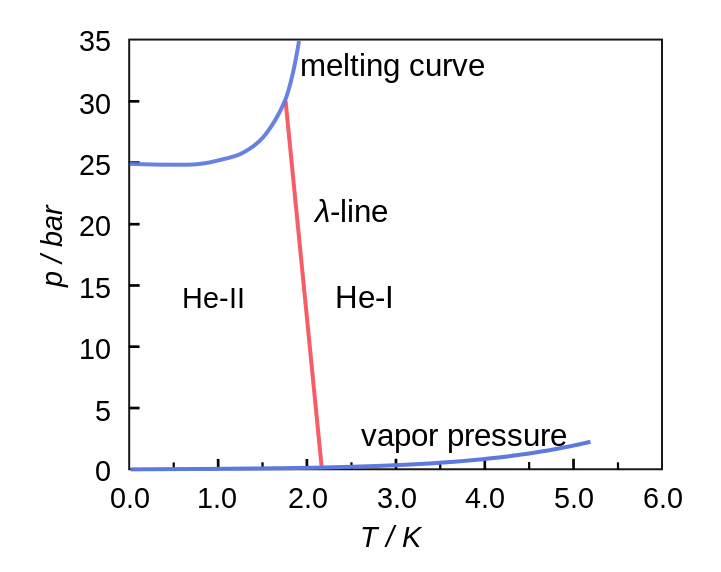
\includegraphics[width=0.7\textwidth]{phasetransition.png}
  \caption{The phase diagram of $^4$He. Here the normal fluid phase or
    He-I and the superfluid phase or H-II are shown.}
\label{fig:phasetransition}
\end{figure}

Because of its zero viscosity, superfluid helium has the ability to
flow through very small capillaries or narrow channels without
experience any friction at all. The flow of liquid helium along the
surface is called film flow.


\subsubsection{Superfluid Helium Converter}

The superfluid $^4$He is an attractive candidate as a UCN source, and
was studied in Ref.~\cite{Golub77}.  It has zero neutron absorption
cross-section, resulting in $\tau_a \rightarrow \infty$, which makes it
a good candidate as a UCN source.  In superfluid helium the upscattering
losses become smaller than $\beta$-decay losses below $T \sim 0.7$~K.
The dominant production mechanism is the excitation of a single phonon
at the crossing of the free neutron and phonon dispersion curves, with
a momentum $q\sim 0.7$/\AA~\cite{Brome2001}, and energy 1~meV
corresponding to a neutron wavelength 8.9~\AA. The availability of
8.9~\AA~cold neutrons is crucial and their flux must be maximized.
%For a long UCN lifetime in superfluid helium, besides the low
%temperature of the converter, the $^3$He contamination must be low
%($^3$He/$^4$He $\le 10^{-12}$), due to its large absorption
%cross-section, which requires $^4$He purification.
There are two types of UCN sources based on superfluid helium: sources
where experiment and source are combined in one apparatus, and the
measurement is performed inside the superfluid helium, and
extracted-UCN sources where the source is an apparatus on its own, and
delivers neutrons to experiments at room temperature connected to it
by UCN guides.



\subsubsection{UCN Production Rate with Single Phonon scattering in
  Superfluid
  helium~\cite{Korobkina2002,Schmidt2009,Golub77}\label{sec:UCN_production}}
UCN can be produced by one phonon excitation in superfluid helium when
the energy of the incident neutrons is equal to that of the one phonon
excitation in the medium. The incident neutrons then scatter down to
UCN by creating one-phonon excitations in the converter medium.
%The crossing of the dispersion curve for excitations in superfluid
%helium and the free energy of the neutron shows that the neutron
%wavelength should be 0.89~nm~\cite{Brome2001} or 8.9~\AA ~in
%order to excite phonon transitions.
\begin{figure}[h!]
\begin{center}
   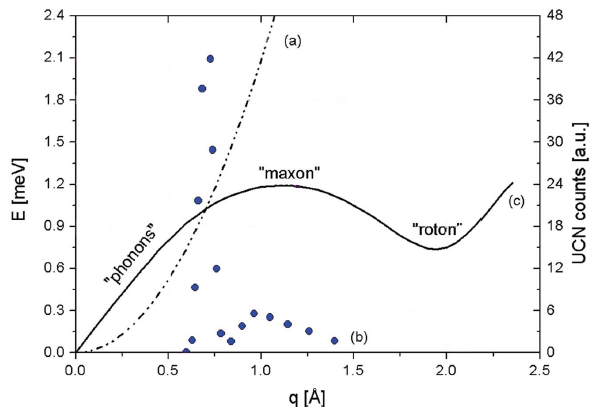
\includegraphics[width=0.7\textwidth]{FIG1_2.PNG}
    \caption{\cite{PSI_news} Dispersion relation of superfluid
      helium~(c) and of the free neutron~(a). Neutrons with $E\simeq
      1$~meV and wavenumber $q \simeq 0.7$/\AA~can excite a single
      phonon with the same energy and momentum and be downscattered to
      UCN energy range. The UCN production rate (b)(circles) shows the
      dominance of this single phonon process with respect to
      multiphonon processes at higher momentum $q$.
%    The two curves cross at $q=0$ and at $q=q^*$, which corresponds
%    to a neutron wavelength of 0.89~nm, oe an energy of 12~K.
    }
%     \vspace{-2.em}
    \label{fig:FIG1}
    \end{center}
\end{figure} 
Fig.~\ref{fig:FIG1} shows the dispersion relation of the superfluid
helium and a free neutron. A neutron at rest can absorb energy $\hbar
\omega$ and momentum $\hbar q$ with
\begin{equation}
\label{neutron_energy}
\omega=\frac{\hbar q^2}{2m},
\end{equation}
where $m$ is the mass of the neutron. A neutron with this energy and momentum can
come to rest after transferring its energy and momentum to the
superfluid $^4$He. For single phonon interactions, which are usually
dominant, the superfluid can only exchange quantities of energy and
momentum that are related by the dispersion curve

\begin{equation}
\label{dispersion_helium}
\omega=\omega(q)= cq,
\end{equation}
where $\omega$ is the energy of the phonon, $q$ is the phonon's
momentum, and $c$ is the speed of sound in the moderator. The second
equal sign in Eqn.~(\ref{dispersion_helium}) is an approximation to
simplify the discussion. The neutrons can only come to rest by
emission of a single phonon, if they have the resonant energy $E_0^*$
given by the intersection of Eqns.~(\ref{neutron_energy}) and
(\ref{dispersion_helium})

\begin{equation}
\omega(q)=cq=\frac{\hbar q^2}{2m},
\end{equation}
and so
\begin{equation}
q^*=\frac{2mc}{\hbar}.
\end{equation}

%Fig.~\ref{fig:FIG1} shows that an incident neutron can lose its
%entire energy by creating a phonon excitation inside the converter
%medium if it has the energy amount equal to the phonon excitations in
%the converter medium. If this energy is $E_0^*=\hbar^2 k_0^*/2m$,
%using Eqns.~(\ref{dispersion_helium}) and~(\ref{neutron_energy}),
%$k_0^*=2mc/ \hbar$.

The differential cross-section for neutron scattering is given by the
dynamic scattering function $S(q,\omega)$, which is the Fourier
transform of the Van Hove correlation function $G(r,t)$ in space and
time of the superfluid helium~\cite{Squires}:

\begin{equation}
\frac{d\sigma}{d\omega}=b^2 \frac{k_2}{k_1}S(q,\omega) d\Omega,
\end{equation}
where $b$ is the bound neutron scattering length for $^4$He,
$\hbar k_1$ is the momentum of the incident neutrons, and
$\hbar k_2=\hbar k_{\text{UCN}}$ is the momentum of UCN. The quantity
$S(q,\omega)$ has been measured in great
detail~\cite{S_func1,gibbs1999collective,S_func3}. Performing the
change of variables,

\begin{equation}
d\Omega=2 \pi \sin \theta d \theta = 2 \pi \frac{q dq}{k_1 k_2}
\end{equation}
gives

\begin{equation}
 \frac{d\sigma}{d\omega}=2\pi b^2 \frac{k_2}{k_1}S(q,\omega)\frac{q
   dq}{k_1 k_2}=2\pi b^2 S(q,\omega)\frac{q dq}{k_1^2}.
\end{equation}
This may effectively be integrated over the limits on $q$ which are

\begin{equation}
k_1-k_2 < q < k_1+k_2.
\end{equation}
Since
\begin{equation}
k_2=k_{\text{UCN}} \ll k_1, \; \; \; \; q\sim k_1 ,
\end{equation}
we may write $dq=2k_{\text{UCN}}$. This results in the cross-section
being related to $S(q,\omega)$ evaluated on the incident neutron's
dispersion curve:

\begin{equation}
\frac{d\sigma}{d\omega}=4\pi b^2 \frac{k_{\text{UCN}}}{k_1}S \left(
k_1, \omega=\frac{\alpha k_1^2}{2} \right),
\end{equation}
where $\alpha=\frac{\hbar}{m}=4.14$~meV/\AA$^2$, and $S(q,\omega)$
assumed to be constant over the narrow range $dq$. The approximation

\begin{equation}
\omega=\frac{\hbar (k_1^2-k_2^2)}{2m}=\frac{\alpha}{2} (k_1^2 -
k_2^2)\approx \frac{\alpha}{2}k_1^2
\end{equation}
has also been used.

The UCN production rate is given by
\begin{equation}
\label{UCN_production}
P(E_{\text{UCN}}) dE_{\text{UCN}} = N_{\text{He}} \int \frac{d\Phi
  (E_1)}{dE}\cdot \frac{d \sigma}{d \omega}(E_1 \rightarrow
E_{\text{UCN}}) dE_1 dE_{\text{UCN}},
\end{equation}
where $\frac{d\Phi (E_1)}{dE}$ is the differential incident neutron
flux, $N_{\text{He}}$ is the atomic density in the liquid helium, and
$\frac{d \sigma}{d \omega}(E_1 \rightarrow E_{\text{UCN}})$ is the
energy differential cross-section for the inelastic neutron scattering
or the probability of the incident neutrons with energy $E_1$ to
scatter from the helium nucleus and become UCN.  Then

\begin{equation}
\label{eqn:He_P_rate}
\begin{split}
\int _0 ^{E_c} P(E_{\text{UCN}})dE_{\text{UCN}} &= N_{\text{He}} 4 \pi b^2
\alpha^2 \left[ \int \frac{d\Phi(k_1)}{dE} S \left( k_1,
  \omega=\frac{\alpha k_1^2}{2} \right)dk_1 \right] \int_0^{k_c}
k_{\text{UCN}}^2dk_{\text{UCN}} \\ &=N_{\text{He}} 4 \pi b^2 \alpha^2 \left[
  \int \frac{d\Phi(k_1)}{dE} S \left( k_1, \omega=\frac{\alpha
    k_1^2}{2} \right) dk_1 \right] \frac{k_c^3}{3}\;
\text{UCN}/\text{cm}^3 \text{s},
\end{split}
\end{equation}
where $E_c$ and $k_c$ are the critical UCN energy and wave vector of
the walls of the storage chamber. This way of writing the UCN
production rate is more general, and it is useful to calculate the
single phonon and multiphonon contributions to the UCN production
rate. The one phonon production rate is found by evaluating
Eqn.~(\ref{eqn:He_P_rate}) over the one phonon peak ($q^*=0.7$/\AA).
Thus
\begin{equation}
P_{\text{UCN}}=9.44 \times 10^{-9}\frac{d\Phi (E_1^*)}{dE_1^*} \;
\text{UCN}/\text{cm}^3,
\end{equation}
 where $E_1^*$ is the energy of the incident neutrons at the one phonon peak.
%\begin{equation} P_{1p}=N4\pi b^2 S^* \alpha \beta
%\frac{k_c^3}{3k^*}\frac{d\Phi (E_1^*)}{dE} \; \text{UCN}/\text{cm}^3
%, \text{s} \end{equation}





% The differential cross-section $\frac{d \sigma}{d E_{UCN}}$ is given
% by \begin{equation} \label{energy_differential_cross_section}
% \frac{d\sigma}{d E_{UCN}}= 4 \pi b^2 \frac{k_{\text{UCN}}}{k_0}S(q,
% \omega) \end{equation} where $b$ is the bound neutron scattering
% length for $^4$He, $k_{\text{UCN}}$ is the UCN momentum and $S$ is
% the Fourier transform of the Van Hove correlation function $G(r,t)$
% in space and time of the superfluid helium~\cite{Squires}.
% Here \begin{equation}
% \omega=\frac{E_0-E_{UCN}}{\hbar} \end{equation} but since $E_0 \gg
% E_{UCN}$, then \begin{equation} \omega \simeq
% \frac{E_0}{\hbar} \end{equation}
% and, \begin{equation} \label{wave_vector_transfer} k_0 -
% k_{\text{UCN}} < q < k_0 + k_{\text{UCN}} \end{equation} where
% $k_{\text{UCN}} \ll k_0$ and therefore $q \simeq k_0$. Therefore
% $\omega=\frac{\alpha k_0^2}{2}$ where $%
% \alpha=\frac{\hbar}{m}=4.14$ meV \AA$^{-2}$. By substituting
% Eqn.~(\ref{energy_differential_cross_section}) to
% Eqn.~(\ref{UCN_production}), the general form of UCN production rate
% will be

% \begin{equation} \label{UCN_Production_rate_helium} P(E_c)= N_{\text{He}} 4
% \pi b^2 \alpha^2 \left[ \frac{d\Phi (k_0)}{dE} S(k_0,\omega) dk_0
% \right] \frac{k_c^3}{3} \end{equation} with the units of UCN
% cm$^{-3}$s$^{-1}$ \cite{Korobkina2002}. $E_c$ and $k_c$ are the
% critical UCN energy and wave vector of the walls of the storage
% chamber.  The UCN density produced by one-phonon excitation in
% superfluid helium was first calculated by Golub and Pendlebury
% \cite{Golub77}. They found a UCN density of $\rho_U\simeq 300$
% n~cm$^{-3}$ for a cylindrical bottle with radius 10 cm and diameter
% 20 cm. This was a substantial improvement over all existing UCN
% sources which yield $\rho\lesssim 1$ n~cm $^{-3}$.

%To achieve such UCN density, the density of $^3$He must be low enough
%so that the neutron absorption by $^3$He does not significantly
%affect the storage time in the vessel.

%In the first UCN production, the UCN output was a factor of 50 lower
%than expected \cite{Ageron1978}.  The UCN production rate (first
%calculated by Pendlebusyin 1982)can be calclated by evaluating
%Eqn.~(\ref{UCN_Production_rate_general}) over the one phonon peak
%which is at $k_0^*=0.7 \AA ^{-1}$.

% \begin{figure}[h!]  \begin{center}
% 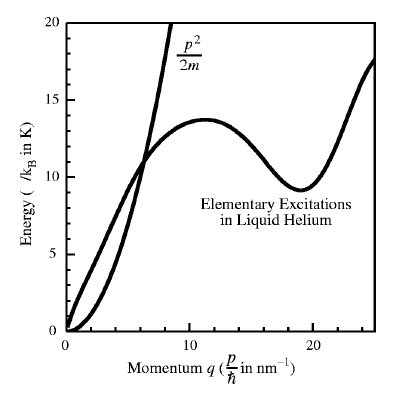
\includegraphics[width=0.5\textwidth]{FIG1.PNG} \caption{The
% dispersion curve for excitations in superfluid helium and the free
% energy of the neutron as a function of momentum transfer
% $q$~\cite{Brome2001}. The two curves cross at $q=0$ and at
% $q=q^*$, which corresponds to a neutron wavelength of 0.89~nm, oe an
% energy of
% 12~K.}  \vspace{-2.em} \label{fig:FIG1} \end{center} \end{figure}



% \item[$\bullet$] why helium? (small neutron absorption cross-section
% ) \item[$\bullet$] UCN production rate in superfluid He calculation
% (Golub77) \item[$\bullet$] Experiment shows the production rate
% matches theory (Ageron1978) and recent UCN rates
% (Zimmer2011) \item[$\bullet$] Experiment design (for example ILL
% design Baker 2003, Masuda2002, PSI source
% Anghel2009) \item[$\bullet$] Temperature of the helium source,
% (below 1K Masuda2012 )

% \item[$\bullet$] UCN storage time in superfluid helium (Golub79)
% \begin{description}



 \subsubsection{Multiphonon Scattering Contribution in UCN Production
   in Superfluid helium~\cite{Korobkina2002,Schmidt2009}}
%So far, the UCN production was demonstrated by single phonon emission. Even though one phonon emission is the predominant process in UCN production for a monochromatic UCN beam, the
 For polychromatic neutron sources, UCN can also be produced by
 multiphonon processes in superfluid $^4$He. Multiphonon production of
 UCN with various energy spectrum of the neutron flux has been studied
 in Ref.~\cite{Korobkina2002}.  Fig.~\ref{fig:Korobkina2002} shows the
 energy spectrum of neutron flux $\frac{d\phi}{dE}$ for three sources
 as a function of momentum $q$, and are compared to the dynamic
 scattering function $S(q,\omega=\hbar q^2/2m)$. The peak at
 $q=0.7$/\AA~corresponds to the one phonon excitation by superfluid
 helium. The values of $S$ above 1.2/\AA~are extrapolated. The value
 of $S$ above 2/\AA~are essentially zero.  The UCN production from one
 phonon and multiphonon processes have been calculated for three input
 neutron spectrums: SNS ballistic guide, PULSTAR MC flux and HMI
 polarized flux.  The multiphonon contribution to the UCN production
 is calculated by using Eqn.~(\ref{eqn:He_P_rate}), and calculating
 $\int \Phi(E_1)S(k_1,\omega=\frac{\alpha k_1^2}{2}) dk_1$.  The
 result showed that, for sources where helium is exposed to the total
 thermal flux or at a dedicated spallation source, the multiphonon
 contribution can amount to slightly more than a factor of 2 increase
 in the UCN production.





\begin{figure}[h!]
\begin{center}
   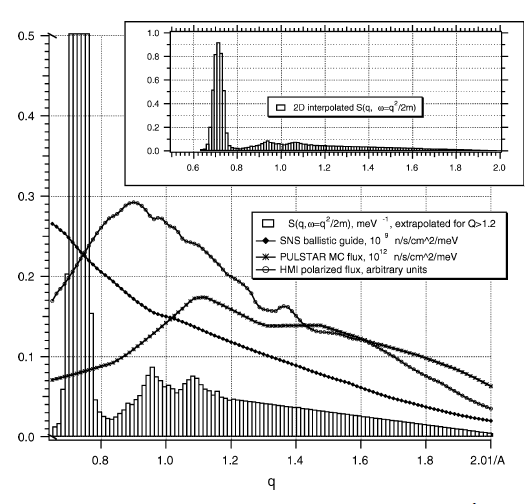
\includegraphics[width=0.7\textwidth]{Korobkina2002.PNG}
    \caption{The energy spectrum of the incident cold neutron flux
      from three sources compared to the dynamic scattering function
      $S(q,\omega=\frac{\alpha k_1^2}{2})$~/meV as a function of
      $q$~/\AA.}
%     \vspace{-2.em}
    \label{fig:Korobkina2002}
    \end{center}
\end{figure} 



%They took the energy spectrum of the neutron flux from three sources
%and extrapolated it for values of $q > 1.2$ \AA $^{-1}$ and they
%compared the results to the scattering function.

%The proposed UCN source at the North Carolina State (NC) locates a
% UCN source in the thermal column of the campus 1-MW PULSTAR reactor
% after removing the graphite. The main point of this design was the
% independence of the UCN production process to the direction of the
% incident neutrons. The proposed UCN source at the Spallation Neutron
% Source (SNS) places a superthermal UCN source on a monochromatic
% 0.89~nm beam at a guide tube. Two types of guides as ``ordinary''
% supermirror guide and ``ballistic'' guide. The ballistic guide has
% more flux at the critical 0.89~nm wavelength but less flux at
% wavelengths shorter than 0.6~nm.  The results are summarized in
% Table~\ref{tab:multiphonon}.  \begin{table} \begin{center} \begin{tabular}{|c|c|c|c|c|c|}
% \hline & NC state & SNS ord & SNS ball & HMI a.u. & Maxwell
% \\ \hline Multi-ph & 490 & 1.0 & 0.94 & 4.7 & 1.7\\ \hline Single-ph
% & 375 & 1.8 & 2.4 & 5.5 & 1.5 \\ \hline Mph/1ph & 1.4 & 0.55 & 0.4 &
% 0.85 & 1.13 \\ \hline \end{tabular} \caption{Predicted production
% rates of UCN from single and multiphonon emission from three sources
% and comparison to Maxwellian
% spectrum} \label{tab:multiphonon} \end{center} \end{table} For the
% NC state proposed UCN source, where the helium is exposed to the
% total thermal flux, the inclusion of multiphonon contribution
% increases the UCN production rate by a little more than a factor of
% 2.

%%%%%%%%%%%%%%%%%%%%%%%%%%%%%%%%%%%%%%%%%%%%%%%%%%%%%%%%%%%%%%%%%%%%%%%%%%%%%%
%% I can get rid of this part
%%%%%%%%%%%%%%%%%%%%%%%%%%%%%%%%%%%%%%%%%%%%%%%%%%%%%%%%%%%%%%%%%%%%%%%%%%%%%%
UCN production by multiphonon emission in superfluid helium under
pressure is studied in Ref.~\cite{Schmidt2009}.  The dynamic
scattering function $S(q,\omega)$ of the superfluid helium strongly
depends on pressure, leading to a pressure-dependent differential UCN
production rate. The expression for the multiphonon part of $S$
describing UCN production is derived from the inelastic neutron
scattering data.  Application of pressure to superfluid helium
increases the velocity of sound, such that the dispersion curves of
the $^4$He and of the free neutron cross at shorter neutron
wavelength.

Since for neutron beams from a liquid deuterium cold source, the
differential flux density $\frac{d\Phi}{dE}$ in the range
8-9~\AA~normally increases for decreasing wavelength of the cold
neutron flux, and also since pressure increases the density of He-II,
it was expected to observe an increase in the single phonon UCN
production rate, and different multiphonon contribution with pressure
increase.  It was observed that, both the single and the multiphonon
scattering functions change with pressure. The single phonon
excitation moves to a shorter wavelength~(see
Fig.~\ref{fig:Schmidt_S}) and the value for $S$ decreases. It leads to
a reduction in one-phonon UCN production.  The multiphonon excitations
increase with pressure, and the peak of the scattering function $S$
moves to shorter incident-neutron wavelengths, see
Fig.~\ref{fig:Schmidt_S}. However, the UCN production rate decreases
with pressure increase.  Only if the cold neutron flux at
8.3~\AA~exceeds by more than 2.5 times that at 8.9~\AA, an increase in
the UCN production rate may be expected. However, it has to be
considered that the application of pressure requires a window for UCN
extraction which causes severe UCN losses. Therefore, UCN production
in superfluid helium under pressure is concluded not to be attractive.




\begin{figure}[h!]
\begin{center}
   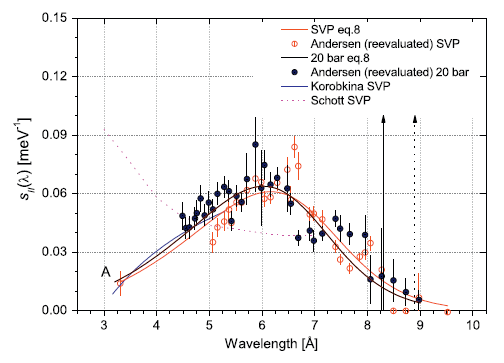
\includegraphics[width=0.7\textwidth]{Schmidt_S.PNG}
   \caption{~\cite{Schmidt2009} Multiphonon scattering function at
     SVP~(Saturated Vapour Pressure) and 20~bar. The extrapolation to
     short wavelength of Korobkina {\it {et al.}}~\cite{Korobkina2002}
     at SVP is linear in $k$, whereas the calculation of Schott {\it
       {et al.}}~\cite{Schott2003} is based on the static structure
     factor of the superfluid helium. The data point ($A$) is taken
     from Ref.~\cite{Fak1991}. The one-phonon peaks are indicated by
     vertical arrows: SVP~(dotted line) and 20~bar~(solid line).  }
%     \vspace{-2.em}
    \label{fig:Schmidt_S}
    \end{center}
\end{figure} 


%%%%%%%%%%%%%%%%%%%%%%%%%%%%%%%%%%%%%%%%%%%%%%%%%%%%%%%%%%%%%%%%%%%%%%%%%%%%%%%


\subsubsection{UCN upscattering and UCN lifetime in superfluid helium~\label{sec:upscattering}}

%%%%%%%%%%%%%%%%%%%%%%%%%
%%% ADD THIS For a long UCN lifetime in superfluid helium, besides the
%%% low temperature of the converter, the $^3$He contamination must be
%%% low ($^3$He/$^4$He $\le 10^{-12}$), due to its large absorption
%%% cross-section, which requires $^4$He purification.
%%%%%%%%%%%%%%%%%%%%%%%%


Superfluid $^4$He has a zero neutron absorption cross-section, and if
the converter is kept at sufficiently low temperatures~(typically
$\lesssim$ 1~K), thermal upscattering of UCN is sufficiently
suppressed. This allows the produced UCN to survive in the converter
for times dominated by the wall losses of the vessel, typically
$>$100~s~\cite{Leung2016}.

The upscattering of neutrons is caused by the interactions between a
neutron at rest, and excitations in superfluid helium at different
temperatures. These excitations can be categorized in three groups:
one phonon absorption, two-phonon scattering, and roton-phonon
scattering. The total upscattering rate can be written as

\begin{equation}
\label{eqn:hE_{UCN}pscattering}
\frac{1}{\tau_{up}} =
\frac{1}{\tau_{1-ph}}+\frac{1}{\tau_{2-ph}}+\frac{1}{\tau_{rot-ph}},
\end{equation}
where 
%which are described by the following equation:
\begin{equation}
\label{eqn:1ph}
\frac{1}{\tau_{1-ph}}= A e^{-(12 K)/T}
\end{equation}
is the one phonon absorption contribution, 

\begin{equation}
\label{eqn:2ph}
\frac{1}{\tau_{2-ph}}= BT^7
\end{equation}
is the two-phonon scattering contribution~(one phonon absorbed and one
phonon emitted), and
\begin{equation}
\label{eqn:ph-rtn}
\frac{1}{\tau_{rot-ph}}= CT^{3/2}e^{-(8.6 K)/T}
\end{equation}
is the contribution from roton-phonon scattering with the absorption
of one roton followed by a phonon emission.

%The first term comes from one phonon absorption, the second term from
%two-phonon scattering where one phonon absorbed and one phonon
%emitted, and the third term from roton-phonon scattering which the
%absorption of one roton followed by a phonon emission.
The values of $A$, $B$ and $C$ are extracted from data for
temperatures up to 2.4~K~\cite{Leung2016}. The comparison between
the UCN production and upscattering rate to the theoretical
temperature dependence of these processes showed that, the main
contribution is from two-phonon scattering $\frac{1}{\tau_{up}}=BT^7$
with $B=(4-16)\times 10^{-3}$~/(s K$^7$)~\cite{Leung2016}.


%The most recent study of the upscattering rates in superfluid helium
%is done by Leung {\it{et al.}}~\cite{Leung2016}.  They calculated
%the upscattering rate due to each individual excitation in a
%temperature range of 0.5~K to 2.2~K as shown in
%Fig.~\ref{fig:Leung2016}. They calculated the $A$, $B$ and $C$
%coefficients for $T \lesssim 1$~K; however, their temperature
%dependencies are weak compared to the overall sizes of the terms.
%They varied the temperature of the converter from 1.2~K to 2.4~K and
%studied the UCN production and upscattering rates. They fit data to
%the theoretical temperature dependencies of these processes and they
%determine the values of $A$, $B$ and $C$. Their analysis showed that
%they only need to include two-phonon scattering meaning
%$\frac{1}{\tau_{up}}=BT^7$ with $B=(4-16)\times 10^{-3}$~/s K$^7$.



% \begin{figure}[h!]  \begin{center}
% 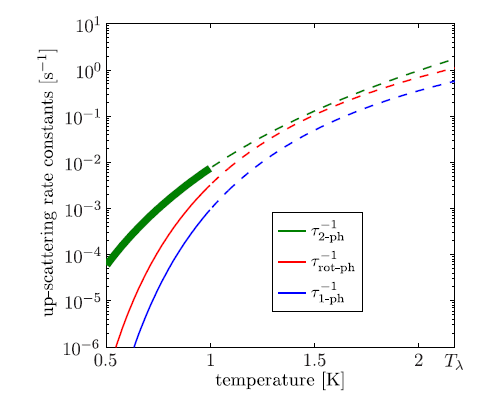
\includegraphics[width=0.5\textwidth]{Leung2016.PNG} \caption{The
% sizes of the three main processes contribution to upscattering of
% UCN by excitations in superfluid % helium from
% Eqn.~(11-14)~\cite{Leung2016}. The thickness of the
% $\tau_{2-ph}^{-1}$ line covers the rnge of values for $T < 1$~K
% owing to the different values of B ($8.8 \times
% 10^{-3}$~s$^{-1}$K$^{-7}$ at 0.6~K and $7.6
% \times10^{-3}$~s$^{-1}$K$^{-7}$ at 1.0~K). The dotted lines are used
% to indicate that the upscattering rates are only approximate for $T
% \gtrsim 1$~K due to temperature dependencies in the $A$, $B$, and
% $C$
% coefficients.}  \vspace{-2.em} \label{fig:Leung2016} \end{center} \end{figure}






%\item[$\bullet$] UCN upscattering in superfluid helium
%(Kilvington1987, Leung2016, Maris1977)


%\subsubsection{UCN lifetime in superfluid $^4$He}

\subsection{UCN production by Solid Deuterium}
Solid deuterium~(sD$_2$) is a material with small absorption
cross-section, small incoherent scattering cross-section~(to minimize
upscattering), and the presence of numerous phonon modes, which can
inelastically scatter neutrons down to UCN energies.
%In solid D$_2$ the phonon excitations are present in the coherent
%part of the scattering, whereas the incoherent part is determined by
%rotational transitions and also by incoherent phonon scattering.
A converter based on sD$_2$ should be operated at temperatures below
10~K in order to avoid subsequent upscattering of UCN by phonons
within solid deuterium.
% The employment of solid deuterium at 10~K increases UCN yield by 10
% times compared with the UCN yield from liquid
% deuterium~\cite{Serebrov2000}.
 
Solid deuterium has an almost perfect hcp crystal structure, when
prepared under suitable conditions~(low pressure and $T >$~5~K). The
D$_2$ molecule has internal rotational modes, which are described by
the rotational quantum number $J$. The rotational excitations give
rise to additional modes in the solid deuterium.
% In the solid phase, $J$ is still a good quantum number.
Deuterium in the states with even $J$ is called
ortho-deuterium~(o-D$_2$), whereas deuterium in the states with odd
$J$ is called para-deuterium~(p-D$_2$). An increase of the
concentration of the p-D$_2$ molecules leads to a larger neutron
upscattering rate.
%The self-conversion between these two species in the solid phase is
%extremely slow compared with the time scale of the experiment and
%therefore, using a para- t ortho- converter is essential.  At low
%temperatures ($T\sim$~6~K), about 99.999\% of the deuterium molecules
%are in the ortho state, when thermal equilibrium is reached. At room
%temperature, D$_2$ has an ortho concentration of 66.7\%.
Theoretically and experimentally, it has been shown that sD$_2$ at
sufficiently low temperatures~(around 5K) with high enough purity and
with high ortho concentration can be used to produce a high density
UCN~\cite{Atchison2005}.

% The common principle is to expose sD$_2$ to a high flux of cold
% neutrons in order to produce UCN. It was shown that, using a pulsed
% neutron beam to produce UCN resulted in densities 4-5 orders of
% magnitude greater than the reactor-based UCN
% sources~\cite{Pokotilovski1995}.  The UCN production rate here
% is a factor of 30 larger as compared to superfluid helium, since the
% phonon spectrum has a much higher phase space density for the
% downscattering of cold neutrons~\cite{Golub83}. The UCN density
% in such sources is limited by nuclear absorption in the converter
% medium, and UCN lifetime.  Below 5K, upscattering in sD$_2$ is less
% important than absorption~\cite{Liu2000}.





\subsubsection{UCN Production Cross-Section and UCN Production Rate in Solid Deuterium~\cite{ucnbook,Frei2010,Frei2009}}

The formula for the UCN production in solid deuterium is very similar
to that of the superfluid helium shown in Eqn.~(\ref{UCN_production}),
with replacing $^4$He atomic density $N_{\text{He}}$ with molecular density
of solid deuterium $N_{D_2}$, and noting that in sD$_2$ the neutron
scattering cross-section may be written as a sum of coherent and
incoherent contributions:

\begin{equation}
\label{eqn:dsigma}
\frac{d\sigma}{d\omega}=\left[ \frac{k_2}{k_1} 
b_{\text{coh}}^2 S_{\text{coh}} (q,\omega) + \frac{k_2}{k_1} b_{\text{inc}}^2 S_{\text{inc}}(q,\omega) \right]
 d\Omega.
\end{equation}
In Ref.~\cite{Frei2010} the UCN production cross-section $\sigma$
was determined by two ways. One way is the determination of the
quasi-particle~(phonons and rotational excitations of the D$_2$
molecule) density of states $G_1(E)$~(incoherent approximation) from
the measured neutron cross-section $\frac{d\sigma}{d\omega}$, and the
other method is the direct integration of the dynamical neutron
cross-section $\frac{d\sigma}{d\omega}$ ($\hbar=1$) in the kinematical
region along the free-neutron dispersion parabola.

\paragraph{UCN production cross-section: Incoherent approximation.}
With the knowledge of the quasi-particle density of states $G_1(E)$,
it is possible to calculate the dynamical neutron cross-section
$\frac{d\sigma}{d\omega}$~(averaged over the scattering angle, thus
$q$). Vice versa it is also possible to extract $G_1(E)$ from a
measured dynamical neutron cross-section~\cite{Turchin}.  If
$G_1(E)$ is known, it is possible to calculate one-phonon and
multiphonon contributions to the neutron cross-section
$\frac{d\sigma}{d\omega}$.
% In the incoherent
% approximation \begin{equation} \label{eqn:G} \frac{d\sigma}{d\omega}=\frac{k_2}{k_1}[b_{eff}(q)]^2 \frac{\hbar
% q^2}{2m}\frac{G(\omega)}{\omega} \left[ n(\omega)+1 \right]
% e^{-2W(q)} \end{equation} where $G(\omega)$ is the generalized
% density of states (GDOS). With the measured inelastic neutron
% cross-section and Eqn.~(\ref{eqn:G}), it is possible to determine
% the GDOS.  $G(\omega)$ comprises the complete phonon excitations of
% sD$_2$ as well as rotational transitions of individual D$_2$
% molecules. Furthermore, multiphonon excitations of the phonon system
% of sD$_2$ should appear in the GDOS as they are not corrected for in
% Eqn.~(\ref{eqn:G}).  GDOS for differently prepared D$_2$ crystals at
% the same o-D$_2$ concentration is measured for o-D$_2$ 66.7\% and
% 95\%~\cite{Frei2009}. The result did not show variations beyond
% statistical effects.  The main difference between the GDOS for
% different o-D$_2$ concentrations was the strength of the rotational
% transition $J=0\rightarrow 1$. Increasing the o-D$_2$ concentration
% enhances this transition.


% The generalized density of states (GDOS) $G(\omega)$ is measured to
% ultimately calculate dynamical neutron cross-section (incoherent
% approximation). $G(\omega)$ comprises the complete phonon
% excitations of sD$_2$ as well as rotational transitions of
% individual D$_2$ molecules. Furthermore, multiphonon excitations of
% the phonon system of sD$_2$ should appear in the GDOS.  GDOS for
% differently prepared D$_2$ crystals at the same o-D$_2$
% concentration was measured for o-D$_2$ 66.7\% and
% 95\%~\cite{Frei2009}. The result did not show variations beyond
% statistical effects.  The main difference between the GDOS for
% different o-D$_2$ concentrations was the strength of the rotational
% transition $J=0\rightarrow 1$.  Increasing the o-D$_2$ concentration
% enhances this transition.
% Fig.~\ref{fig:Frei2010fig}~\cite{Frei2010} shows two examples of
% neutron scattering data for two different concentrations of o-D$_2$
% molecules as a function of energy transfer $E=E_i-E_f$.  The density
% of state (DOS) $G_1$ can be extracted from GDOS data, and it leads
% to the calculation of $d\sigma/dE$. Studies showed
% that~\cite{Frei2010}, an increase in the concentration of the
% p-D$_2$ molecules leads to a larger neutron upscattering.  This
% upscattering has serious implications to the upscattering of UCN in
% the sD$_2$ converter material, and reduces the achievable density of
% UCN in sD$_2$.  It is also shown that, the elastic cross-section
% ($E=$0~meV) of sD$_2$ is quite large.  The one-particle excitation
% on the dynamic neutron scattering cross-section is above E$=$10~meV,
% two-particle contributions is above E$\sim$5~meV, and three particle
% excitations above E$=$12~meV~\cite{Frei2009}.
The method for the determination of $G_1(E)$ from the measured neutron
scattering data in solid deuterium is studied in
Ref.~\cite{Frei2009}. In the determination of $G_1(E)$, contributions
of higher order multiphonons to $\frac{d\sigma}{dE}$ are incorporated.

In the case of UCN production, the energy transfer of the
downscattered neutron $E=E_1-E_{\text{UCN}}$ is approximately equal to
the initial neutron energy $E_1$
($E_{\text{UCN}} \ll E_1, E_{\text{UCN}}$: UCN energy). The total
cross-section for UCN production can be calculated by

\begin{equation}
\sigma_{\text{UCN}}({E_1})=\int_0 ^{E_{\text{UCN}}^{max}} \frac{d\sigma (E_1)}{dE} dE_{\text{UCN}}.
\end{equation}

The calculated cross-section shown in
Fig.~\ref{fig:Frei2010_sigma_G1}, is in agreement with data on UCN
production using a cold neutron beam~($E_1 \sim 1.4$~meV to 20~meV).
Here the one-quasi-particle and two-quasi-particle excitations are
included in the calculations.  The UCN production cross-section is
mainly determined by one-quasi-particle excitation for energies below
15~meV. The two-quasi-particle contribution is non-negligible in the
region of 5-25~meV.

The application of the incoherent approximation in the case of sD$_2$
has certainly to be questioned since the sD$_2$ crystal scatters
neutrons more coherently than incoherently.

\begin{figure}[h!]
\begin{center}
   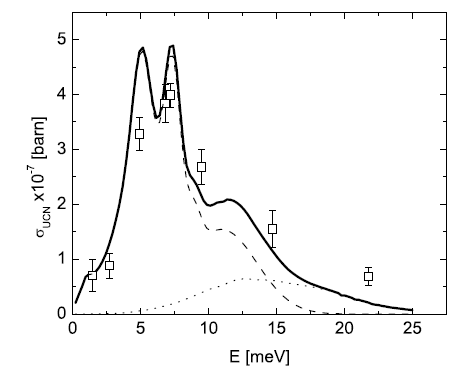
\includegraphics[width=0.5\textwidth]{Frei2010_sigma_G1.PNG} \caption{UCN
    production cross-section of sD$_2$ with 98\% ortho
    concentration. UCN energy range 0-150~neV inside the solid
    D$_2$. Solid line: cross-section calculated in incoherent
    approximation. Dashed line: one-quasi-particle
    contribution. Dotted line: two-quasi-particle
    contribution. $\square$: data from measurements at
    PSI~\cite{Atchison2007}.  }
%     \vspace{-2.em}
    \label{fig:Frei2010_sigma_G1}
    \end{center}
\end{figure} 




\paragraph{UCN production cross-section: Direct determination.}
The easiest way of determining the cross-section for UCN production is
the use of the dynamical scattering function $S(q,\omega)$ in the
($q,\omega$)-phase space along the free-neutron parabola, as shown
schematically in Fig.~\ref{fig:sD2_S}.

This method allows the incorporation of all the coherent and
incoherent contributions to the UCN production cross-section. Possible
coherent contributions, which cannot be treated exactly with the
incoherent approximation, appear directly in the deduced
cross-section. Therefore, this method is superior in principle to the
result obtained by the incoherent approximation.

\begin{figure}[h!]
\begin{center}
   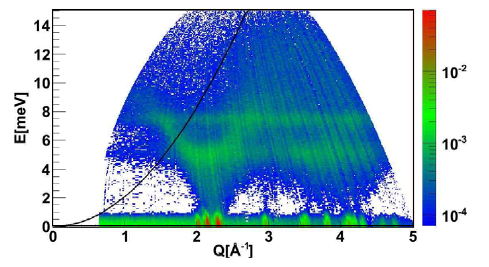
\includegraphics[width=0.7\textwidth]{sD2_S.PNG} \caption{\cite{Frei2010}
    $S(q,\omega)$ ($q=Q ,\omega=E$) (arb. units) of 95.2\% solid
    o-D$_2$ at $T=4$~K. Data from IN4 measurements. Black parabola:
    dispersion of the free neutron. }
%     \vspace{-2.em}
    \label{fig:sD2_S}
    \end{center}
\end{figure} 



The UCN production cross-section can be determined by
\begin{equation}
\sigma_{\text{UCN}}(E_1)=\frac{\sigma_1}{k_1} S(k_1, E_1) \frac{2}{3} k_{\text{UCN}}^{max} \; E_{\text{UCN}}^{max} ,
\end{equation}
where $E_1$ is the energy of the incoming neutrons in the
downscattering process, $\sigma_1$ is a constant, and
$k_{\text{UCN}}^{max}$ and $E_{\text{UCN}}^{max} $ are the upper
limits for the UCN momentum and energy.  In order to obtain absolute
cross-sections, $S(q,\omega)$ has to be calibrated to absolute values.
The result of this calibration and the determination of the UCN
production cross-section as a function of the energy of the incoming
neutrons, and a comparison with the measurements of this cross-section
is shown in Fig.~\ref{fig:Frei2010fig2}. This plot also contains the
data, which were obtained with higher incoming-neutron energy
($E_1=67$~meV).


\begin{figure}[h!]
\begin{center}
  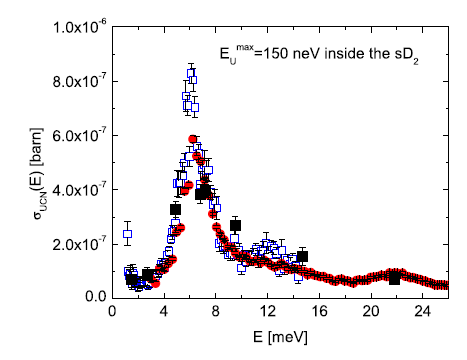
\includegraphics[width=0.5\textwidth]{Frei2010_sigma.PNG} \caption{\cite{Frei2010}
    UCN production cross-section solid o-D$_2$ of
    95.2\%~\cite{Frei2010}. A UCN energy range of 0-150~neV inside the
    solid D$_2$ is assumed. Sample: fast frozen solid deuterium
    ($T=4$~K); data from IN4 measurements. Blue $\square$:
    $E_0=17.2$~meV. Red filled $\bigcirc$: $E_0=67$~meV,
    $\blacksquare$: direct UCN production data from measurements at
    PSI~\cite{Atchison2007}.  }
%     \vspace{-2.em}
    \label{fig:Frei2010fig2}
    \end{center}
\end{figure} 

The comparison of the calculated UCN production cross-section,
extracted from the incoherent approximation and parabola method, shows
(see Fig.~\ref{fig:Frei2010_sigma_G1} and Fig.~\ref{fig:Frei2010fig2})
a discrepancy in the region of $E\sim6$~meV.  The cross-section
determined by the parabola method shows a pronounced maximum in the
region of $E\sim6$~meV as compared to the incoherent approximation
result. This peak corresponds to the coherent phonon contribution to
the UCN production cross-section. The double-peak structure in the UCN
production cross-section by the incoherent approximation is not
present in Fig.~\ref{fig:Frei2010fig2}, and cannot be reproduced by the
measured data shown in Figs.~\ref{fig:Frei2010_sigma_G1}
and \ref{fig:Frei2010fig2}.  This means, a new experiment at a more
intense cold neutron beam with a better energy resolution would be
desirable to study this effect further.

In Fig.~\ref{fig:sD2_S}, the parabola of the free neutron crosses the
acoustical phonon dispersion curve at $E \sim 6$~meV. At this point,
the UCN production cross-section is predominantly determined by
coherent scattering.  This can explain a deviation from the production
cross-section in incoherent approximation. Nevertheless, the general
agreement of the incoherent approximation with the PSI data is
remarkable~(as shown in Fig.~\ref{fig:Frei2010_sigma_G1}).


%The coherent phonon contribution to the UCN production cross-section
%at $E \simeq 5$~meV, which is clearly seen in
%Fig.~\ref{fig:Frei2010fig2}, is a major downscattering channel for
%UCN production.

The result for the calculated UCN production rate in solid o-D$_2$,
exposed to a Maxwellian shaped neutron flux for different effective
neutron temperatures is shown in
Fig.~\ref{fig:sD2_production_rate}. The main conclusion from these
results was the new understanding of possible higher energetic loss
channels~(one-quasi-particle and two-quasi-particle) in solid
deuterium for the downscattering of cold neutrons in the conversion
process to UCN. The best value for the effective neutron temperature
is in the region of $T_n \sim 40$~K which is larger than what was
previously expected~($T_n \sim 30$~K~\cite{Yu1986}).


%%%%%%%%%%%%%%%%%%%%%
\begin{figure}[h!]
\begin{center}
  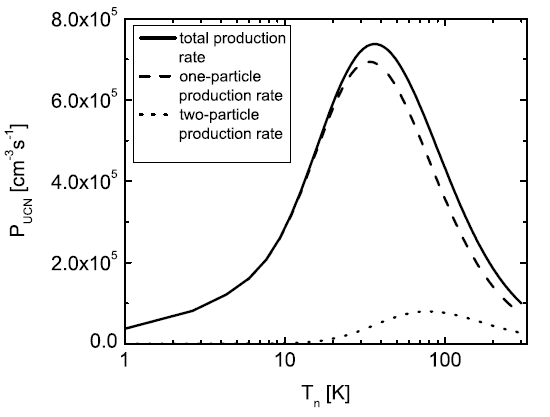
\includegraphics[width=0.5\textwidth]{Frei2010_P.PNG} \caption{\cite{Frei2010}
    Calculated UCN production rate of sD$_2$ with 98\% ortho
    concentration for different Maxwellian neutron spectra with
    effective neutron temperature $T_n$. UCN energy range:0-150~neV
    inside the sD$_2$. Neutron capture flux $10^{14}$~/cm$^2$s. Solid
    line: total production rate~(one- and two- particle
    excitations). Dashed line: one-particle production rate. Dotted
    line: two-particle production rate.}
%     \vspace{-2.em}
    \label{fig:sD2_production_rate}
    \end{center}
\end{figure} 





% \subsubsection{Neutron scattering study} Neutron scattering is an
% excellent tool to investigate the phonon system and the rotational
% transitions of D$_2$ molecules in sD$_2$.  The dynamics of sD$_2$ is
% studied by means of inelastic scattering (coherent and incoherent)
% of thermal and cold neutrons at different temperatures and
% para-ortho ratios~\cite{Frei2009}.  Scattering of neutrons where
% a rotational transition ($ J \rightarrow J^{\prime}$ and $J \neq
% J^{\prime}$) is involved leads to an incoherent response of the
% system. The phonon excitations are present in the coherent part of
% the scattering, whereas the incoherent part is determined by
% rotational transitions and also by incoherent phonon scattering.


% The generalized density of states (GDOS) $G(\omega)$ is measured to
% ultimately calculate dynamical neutron cross-section (incoherent
% approximation). $G(\omega)$ comprises the complete phonon
% excitations of sD$_2$ as well as rotational transitions of
% individual D$_2$ molecules. Furthermore, multiphonon excitations of
% the phonon system of sD$_2$ should appear in the GDOS.  GDOS for
% differently prepared D$_2$ crystals at the same o-D$_2$
% concentration was measured for o-D$_2$ 66.7\% and
% 95\%~\cite{Frei2009}. The result did not show variations beyond
% statistical effects.  The main difference between the GDOS for
% different o-D$_2$ concentrations was the strength of the rotational
% transition $J=0\rightarrow 1$.  Increasing the o-D$_2$ concentration
% enhances this transition.
% Fig.~\ref{fig:Frei2010fig}~\cite{Frei2010} shows two examples of
% neutron scattering data for two different concentrations of o-D$_2$
% molecules as a function of energy transfer $E=E_i-E_f$.  The density
% of state (DOS) $G_1$ can be extracted from GDOS data, and it leads
% to the calculation of $d\sigma/dE$. Studies showed
% that~\cite{Frei2010}, an increase in the concentration of the
% p-D$_2$ molecules leads to a larger neutron upscattering.  This
% upscattering has serious implications to the upscattering of UCN in
% the sD$_2$ converter material, and reduces the achievable density of
% UCN in sD$_2$.  It is also shown that, the elastic cross-section
% ($E=$0~meV) of sD$_2$ is quite large.  The one-particle excitation
% on the dynamic neutron scattering cross-section is above E$=$10~meV,
% two-particle contributions is above E$\sim$5~meV, and three particle
% excitations above E$=$12~meV~\cite{Frei2009}.



% \begin{figure}[h!]  \begin{center} 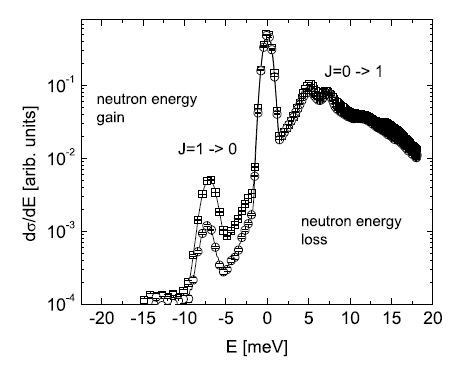
\includegraphics[width=0.5\textwidth]{FREI2010.PNG} \caption{An
%    example of the dynamical neutron cross-section of solid deuterium
%    at T$=7$~K. Comparison of two ortho concentrations c$_0$=66.7\%
%    ($\square$) and c$_0$=98\% ($\bigcirc$). Data from TOFTOF
%    measurements at the FRM II. Initial energy of the thermal
%    neutrons is E$_0=$20.4~meV~\cite{Frei2010}. }
%%     \vspace{-2.em}
%     \label{fig:Frei2010fig}
%     \end{center}
% \end{figure} 





\subsubsection{UCN upscattering and UCN lifetime in sD$_2$~\cite{Liu2000,Morris2002}}


The different molecular species, ortho-D$_2$ and para-D$_2$, have
significantly different UCN-phonon annihilation
cross-sections~\cite{Liu2000}. The presence of even small
concentrations of para-D$_2$ can dominate the upscattering rate which
gives rise to reduced UCN lifetimes in the solid and orders of
magnitude reduction in the achievable UCN density.  In a D$_2$ solid,
the populations of ortho and para states are typically determined by
the ortho/para population of the gas phase before the D$_2$ is frozen
into solid.  After cooling down the D$_2$ to the solid phase
($T \sim$~6~K), it normally takes months to reach the equilibrium of
99.999\% o-D$_2$.
 %The selfconversion between these two species in the solid phase into
 %a thermal Boltzman distribution is extremely slow compared with the
 %time scale of experiment.
Since the elimination of para-D$_2$ is necessary to achieve UCN
lifetimes comparable to the nuclear absorption time in solid
deuterium, using a para-D$_2$ to ortho-D$_2$ converter is crucial.


\begin{figure}[h!]
\begin{center}
  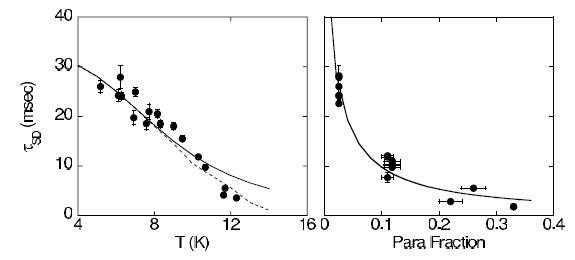
\includegraphics[width=0.8\textwidth]{Morris2002.PNG} \caption{\cite{Morris2002}
    Left- Data points are measured sD$_2$ lifetimes as a function of
    temperature, with the para-fraction fixed at 2.5\%. Only the
    statistical errors are shown. Solid lines show the predicted
    temperature dependence. The dashed line is the predicted effect of
    departure from the solid lifetime model due to the upscattering
    from the D$_2$ gas in the guide. Right- sD$_2$ lifetimes as a
    function of para-fraction for all of the data taken below 6~K. The
    solid line is the model prediction of the para-fraction dependence
    at an average temperature of 5.6~K.  }
%     \vspace{-2.em}
    \label{fig:Morris2002}
    \end{center}
\end{figure} 



%\subsubsection{UCN lifetime in sD$_2$}
The lifetime of the UCN in sD$_2$ is limited by factors such as
upscattering from phonons in the solid, upscattering from p-D$_2$
contamination, and absorption inside the vessel.  Reducing the time UCN
spend inside the sD$_2$ can reduce the average absorption rate. This
led to the proposal of a thin-film source where a thin layer of solid
D$_2$ coats the inside of a storage bottle that is embedded in a cold
neutron flux~\cite{Golub83}. The possibility of a smaller source
volume combined with the higher operating temperature of the thin film
source offers significant technical simplification.

The UCN lifetime in the solid deuterium as a function of the temperature
and para/ortho fractions has been measured~\cite{Morris2002}. The
total loss rate can be written as

\begin{equation}
\label{eqn:SD_lifetime}
\frac{1}{\tau_{SD}}=\frac{1}{\tau_{phonon}}+\frac{1}{\tau_{para}}+\frac{1}{\tau_{Dabs}}+ \frac{1}{\tau_{Habs}},
\end{equation}
where $\frac{1}{\tau_{phonon}}$ is the upscattering rate from phonons
in SD$_2$, $\frac{1}{\tau_{para}}$ is the upscattering rate from para
deuterium molecules in the solid, $\frac{1}{\tau_{Dabs}}$ is the
upscattering rate from the absorption on deuterium and
$\frac{1}{\tau_{Habs}}$ is the upscattering rate from the absorption
on the hydrogen impurities in the solid. The results for UCN lifetimes
$\tau_{SD}$ in sD$_2$ as a function of the sD$_2$ temperature and
para/ortho fractions are shown in Fig.~\ref{fig:Morris2002}. The
difference between the solid and dashed line demonstrates the need to
include the effect of deuterium vapour in the guide on the lifetime at
higher temperatures. With this correction, the measured lifetimes
agree well with theoretical predictions of the upscattering rate.





%They demonstrated the necessity of including the effect of deuterium
%vapor in the UCN guide on the lifetime at higher temperatures to
%achieve an agreement with the theoretical predictions of UCN
%lifetime.  The storage time for UCN in the presence of an exit hole
%is $1/\tau_{tot}=1/\tau_{h}+1/\tau_0$ where $1/\tau_{h}$ is the loss
%rate of UCN through exit hole and $\tau_0$ is the storage time in the
%absence of the hole.  (????? not convincing for the next line!!!!! I
%need to add something here.)

%
%The temperature should be low enough so that the absorption in the film is greater than the upscattering rate.

%\item[$\bullet$] why deuterium? (weak neutron absorption
%cross-section from UCN book and Atchison2005,
%Altarev1980) \item[$\bullet$] UCN production with solid Deuterium
%(Frei2007 and Lauer2013 for Mainz and Morris2002 and Saunders2013 for
%Los Alamos) \item[$\bullet$] upscattering rates
%(Liu2000) \item[$\bullet$] thin film sources?? ( in the UCN
%book) \item[$\bullet$] production of UCN at pulsed neutron source
%(Pokotilovski1995)
\subsection{Comparison between sD$_2$ and superfluid helium sources}

The main differences between sD$_2$ and superfluid helium sources are
the UCN lifetime and the UCN production rate. While UCN can stay in
superfluid helium until it $\beta$-decays, UCN in solid deuterium are
absorbed by the deuteron in 150~ms after they are produced.  Once a
superfluid helium source is cooled down to temperatures below 0.75~K,
the upscattering rate is suppressed to a level comparable to neutron
$\beta$-decay.  Solid deuterium has a production rate two orders of
magnitude greater than superfluid helium. Therefore, solid deuterium
sources output higher UCN current compared to superfluid helium
sources. However, the limiting production time in superfluid helium is
four orders of magnitude longer than sD$_2$. Thus, even with a smaller
UCN production rate, superfluid $^4$He can in principle achieve a UCN
density larger than that of solid deuterium.  The superthermal
enhancement in solid deuterium is limited by the large nuclear
absorption loss, and thus further cooling below 5~K will not
significantly enhance the UCN yield.

%Both types of sources use quantum excitations in the converter medium
%to create the UCN; these are phonons in the case of sD$_2$ and
%phonons and rotons in the case of superfluid $^4$He. Since $^4$He
%does not capture neutrons and has a small upscattering probability
%for UCN, the superfluid $^4$He source can be operated at lower
%currents for longer times, allowing a large density of neutrons to
%accumulate. Storage times of hundreds of seconds are
%achievable. Solid deuterium sources, on the other hand, must pulse
%the beam, then quickly isolate any UCN produced from the sD$_2$,
%usually with a valve directly above the deuterium, because a UCN in
%sD$_2$ will only survive for tens of milliseconds.  The TRIUMF's
%technology is therefore complementary to spallation sD$_2$ projects.






%While the thin film source produces lower UCN densities than the
%helium-based source, the ability of this source to operate with
%shorter storage times without further loss of UCN density will allow
%either a large beam area or a smaller source volume or some
%combination.
\subsection{Other UCN Sources~\cite{Salvat2013,Atchison2009,Liu_thesis}}

Superthermal UCN sources may be compared by

\begin{equation}
\sigma_s / \sigma_a,
\end{equation}

where $\sigma_s$ is the elastic scattering cross-section, and
$\sigma_a$ is the absorption cross-section. At low energies ($<$~1~eV)
$\sigma_a \sim 1/v$ where $v$ is the speed of the neutrons. This
means, the absorption cross-section is much larger at lower energies.
Table~\ref{tab:other_sources} shows a list of possible superthermal
UCN sources~\cite{Liu_thesis}. The values of $\sigma_a$ are for
thermal neutrons.


\begin{table}
\begin{center}
\begin{tabular}{|l|l|l|}
\hline
Isotope & $\sigma_a$(barns) & $\sigma_s / \sigma_a$  \\
\hline
$^2$D & 0.000519 & 1.47 $\times 10^4$ \\
\hline
$^4$He & 0 & $\infty$ \\
\hline
$^{15}$N & 0.000024 & 2.1 $\times 10^5$ \\
\hline
$^{16}$O & 0.00010 & 2.2 $\times 10^4$ \\
\hline
$^{208}$Pb & 0.00049 &  2.38 $\times 10^4$\\
\hline
\end{tabular}
\end{center}
\caption{Candidates for a superthermal source\label{tab:other_sources}}
\end{table}

Solid $\alpha - ^{15}$N$_2$ is a potential alternative to
deuterium~\cite{Salvat2013}. Its absoption cross-section is only 5\%
of that of D$_2$, and it has a negligible incoherent scattering
cross-section. Additionally, rotation of the N$_2$ molecules in the
lattice is inhibited due to the anisotropy of the N$_2$
inter-molecular potential. This leads to the dispersive modes for the
rotational degrees of freedom~(librons), which provide additional
channels for neutron downscattering, and eliminates the rotational
incoherent upscattering. Measurements~\cite{Salvat2013} show that, the
production cross-section peaks near 6~meV, and the optimal incident
cold neutron temperature is 40~K. It was found that, the variation in
the cross-section is no more than 18\% in the range from 5 to
25~K~(increasing slightly with increasing temperature). The measured
cross-section was found to be somewhat lower than that of D$_2$ and
O$_2$.
%However, it has a longer mean free path compared to deuterium.
A nitrogen-based source may benefit from operating at lower
temperatures, if the upscattering cross-section can be further reduced
at lower temperatures~($\sim$1~K)~\cite{Salvat2013}.


$^{208}$Pb and solid deuterium have similar nuclear absorption
cross-sections. The natural solid form of $^{208}$Pb would avoid the
difficulties of growing cryogenic solids such as deuterium and
oxygen. However, its heavy mass prevents the neutron momentum transfer
to the solid phonon field. The heavy mass reduces the phonon creation
cross-section by $1/M$. As a result, one would expect its UCN yield to
be two orders of magnitude less than solid deuterium.

As other options, the properties of the new candidate converter
materials including solid heavy methane~(CD$_4$) and solid
oxygen~(O$_2$) have been investigated in the temperature range 8~K to
room temperature by measuring the production of UCN from a cold
neutron beam and the cold neutron transmission through the converter
materials~\cite{Atchison2009}. The liquid O$_2$, D$_2$ and CD$_4$ have
similar neutron scattering cross-sections.

$^4$He and D$_2$ are still the best commonly pursued options, although
there is a chance that other materials could lead to a breakthrough.
% \item[$\bullet$] Investigationofsolid D$_2$, O$_2$ and CD$_4$ for
% UCN production (Atchison2009) \item[$\bullet$] Investigating solid
% $\alpha$-$^{15}$N$_2$ as a new source of ultra-cold neutrons
% (Salvat2013) \item[$\bullet$] solid $\alpha$-oxygen (Gutsmiedl2011,
% Liu thesis)



% \subsubsection{UCN Production Rate with Single Phonon scattering in
% Superfluid helium} Golub and Pendlebury 1975 and 1977

% \subsubsection{Multiphonon Scattering Contribution in UCN Production in Superfluid helium}
% Korobkina {\it{et al.}} and Schott {\it{et al.}}

% \subsubsection{Neutron Upscattering Rate in Superfluid helium}
% Leung {\it{et al.}} and Maris {\it{et al.}}


% \subsubsection{UCN Production Rate with SD$_2$ converter}



% \subsubsection{UCN Upscattering Rate in SD$_2$}
% Liu {\it{et al.}}



% \section{UCN Extraction}
% Cut if possible


\section{Current Status of UCN sources Worldwide}
%\subsection {It needs to be modified}
New UCN sources using superthermal technology are under development at
various laboratories across the world. Neutrons are produced by two
methods: proton-induced spallation off a heavy nuclear target (e.g.,
tungsten), and fission where neutrons are produced by a nuclear
reactor. Table~\ref{tab:full_ucn_sources}%~\cite{Jeff_dnp}
shows a list of the present and future UCN sources worldwide.



\begin{table}[h!]
\begin{center}
\begin{tabular}{|l|l|l|l|}
\hline
Name & Source Type & Technology & Status \\
  \hline
  \hline
ILL  & Turbine & Reactor, CN beam & Running
%39 & few s 
\\
\hline
%J-PARC & Doppler SHifter & Spallation & Running
%\\
%\hline
ILL SUN-2 & LHe & Reactor, CN beam & Running 
%$\sim$15 peak (60~s,30~L) & 200(4~L, Fomblin grease, 80~neV)
\\
\hline
ILL SuperSUN & LHe & Reactor, CN beam & Future
%$\sim$150 peak (60~s, 30~L)& 800 %(12~L, 230~neV magnetic trap)
\\
\hline
%RCNP/KEK & LHe & Spallation & 26 & 81 (Ni) \\
%\hline
RCNP/TRIUMF/KEK & LHe & Spallation & Installing/Future
%600 polarized & 100 (NiP)
\\
\hline
PNPI Gatchina & LHe & Reactor & Future
%12000 & 10 (from He at 1.2~K)
\\
\hline
%ILL Turbine & sD$_2$ & Turbine & 39 & Few s \\
%\hline
LANL & sD$_2$ & Spallation & Running/Upgrading
%$\sim$25 polarized & 40 
\\
\hline
PSI & sD$_2$ & Spallation & Running
%Peak$\sim$23 & $\sim$90~s
\\
\hline
Mainz & sD$_2$ & Reactor & Running
%10 & Few s
\\
\hline
FRM II, Germany & sD$_2$ & Reactor & Future
%$\sim$5000 & Few s
\\
\hline
NCSU PULSTAR & sD$_2$ & Reactor & Installing
%$>$30 & Few s
  \\
  \hline
  SNS, Oakridge & LHe & Spallation & Future
  \\
  \hline
  J-PARC & Doppler Shifter & CN beam & Running
  \\
  \hline
\end{tabular}
\end{center}
\caption{Existing and future UCN sources worldwide. The existing or
  proposed sources at the following sites is listed: Institut
  Laue-Langevin~(ILL) in France, Reasearch Center for Nuclear
  Physics~(RCNP) in Japan, KEK and J-PARC in Japan, TRIUMF in Canada,
  Petersburg Nuclear Physics Institute~(PNPI) in Russia, Los Alamos
  National Lab~(LANL), PULSTAR and SNS in the US, Mainz and FRM II in
  Germany. }
\label{tab:full_ucn_sources}
\end{table}


Reactor sources place the moderators close to the reactor core~(FRM~II
and Gatchina~\cite{Serebrov_ascona}), or use existing CN beam
lines~(ILL~\cite{Piegsa2014}). At FRM~II, the sD$_2$ will be placed
around a solid hydrogen cold-moderator close to the fuel element. The
Gatchina superfluid $^4$He source will be placed inside their thermal
column, using immense pumping power to cool the converter to 1.1~K,
making rapid extraction necessary due to increased UCN upscattering at
this temperature.

The SuperSUN and SUN-2 experiments are the logical extensions of the
early superthermal source geometry at ILL.  A novel feature of the
SuperSUN experiment at ILL~\cite{Zimmer2015} is a magnetic multipole
reflector for a drastic enhancement of the UCN density with respect to
an existing prototype superfluid helium UCN source installed in a cold
neutron beam. A multipole magnet can lead to a large gain in the
saturated density of low-field-seeking UCNs because the presence of
the field reduces the number of neutrons hitting the material walls
and reduces the energy and wall collision rate of those that do. In
addition, it acts as a source-intrinsic UCN polarizer without need to
polarize the incident beam, and hence avoiding associated losses.
%This concept will lead to a drastic improvement of previous UCN
%storage time constants and hence provide a polarised UCN density
%beyond 1000 per cm$^3$.

The Los Alamos solid deuterium source~\cite{Ito_ascona} uses a
proton beam of 900~MeV and a W target to produce neutrons. The
neutrons get cooled down in a polyethylene cold moderator. The new
design includes a flapper valve to isolate the neutrons from the
sD$_2$ after the proton beam pulse.

The PSI UCN source~\cite{Ries_ascona} uses a 600~MeV proton beam
to hit a Pb/Zr target for neutron production. They use a 30~L volume
of sD$_2$ at 5~K as moderator and converter to produce UCN. This
volume is surrounded by D$_2$O thermal moderator. They also use a
flapper valve for UCN extraction between the proton beam pulses to
limit the losses. The UCN production has been running since 2012 with
an on-going EDM experiment, with a peak density of 23~UCN/cm$^3$.

The Mainz UCN source~\cite{Karch2014} is the only source that
operates at a low power university reactor, and is the newest
production source. The solid deuterium converter with a volume of $V =
160$~cm$^3$, which is exposed to a thermal neutron fluence of 4.5
$\times 10^{13}$~n/cm$^2$, delivers up to 240000 UCN~($v \leq$ 6~m/s)
per pulse outside the biological shield at the experimental area.  UCN
densities of $\approx$ 10/~cm$^3$ are obtained in stainless-steel
bottles of $V \approx$ 10~L. Their pulsed operation permits the
production of high densities for storage experiments.


At the SNS UCN source, the 8.9~$\AA$ cold neutrons are selected using
a monochromator, and are transported with neutron guides to two cells
made out of acrylic~(ultraviolet transmitting) and separated by a high
voltage electrode.  The neutrons entering the cell are
polarized. Within the cell, the cold neutrons become ultra-cold
neutrons via $^4$He single-phonon process~\cite{kolarkar2010}.


The UCN source at J-PARC is a doppler-shifter type of pulsed UCN
source~\cite{Imajo2015}. Very cold neutrons~(VCNs) with 136~m/s
velocity in a neutron beam supplied by a pulsed neutron source are
decelerated by reflection on a wide-band multilayer mirror, yielding
pulsed UCN. The mirror is fixed to the tip of a 2,000~rpm rotating arm
moving with 68~m/s velocity in the same direction as the VCN. The
repetition frequency of the pulsed UCN is 8.33~Hz and the time width
of the pulse at production is 4.4~ms. In order to increase the UCN
flux, a supermirror guide, wide-band monochromatic mirrors, focus
guides, and a UCN extraction guide have been newly installed or
improved. This source will be used to search for the nEDM.


The current UCN source at TRIUMF uses a W target to produce spallation
neutrons from a 500~MeV proton beam on site. The cold neutrons are
converted to UCN in superfluid helium.  The future UCN source is
projected to compete with the capabilities of the best planned future
UCN sources. If TRIUMF's estimated UCN density of 680 UCN cm$^{-3}$ is
achieved, it will be a new world record.

Other sources and nEDM experiments aim at similar goals of hundreds to
thousands of UCN cm$^{-3}$ in the measurement volume. However, to
date, superthermal sources have not produced considerably more UCN
than the ILL turbine source.


% Russ said: "This paragraph could be part of the conclusion.  The
% first paragraph should summarize what a superthermal source is and
% the main differences between He and sD2.  Then this paragraph.
 


%The neutrons are neutral particles, subjected to all fundamental
%forces which helps to investigate the physics beyond the standard
%model.

\section{Summary}
Precision experiments involving UCN provide an attractive avenue to
investigate physics beyond the standard model. Measurement of the
neutron EDM is an example of such experiments. For such studies high
densities of UCN are needed.

UCN are very slow neutrons with velocities $<8$~m/s that can be
trapped in matter, magnetic and gravitational fields.  Superthermal
UCN sources could produce high densities of UCN. Such sources should
have a very small neutron absorption cross-section and upscattering
rate, while having a high UCN production rate. So far, the best
candidates are superfluid helium and solid deuterium.
%The UCN production rate, the upscattering rate and the UCN lifetime
%of $^4$He and sD$_2$ are discussed in detail.

Both $^4$He and solid D$_2$ UCN sources use quantum excitations in the
converter medium to create the UCN; these are phonons in the case of
superfluid sD$_2$ and phonons and rotons in the case of $^4$He. Since
$^4$He does not capture neutrons, and has a small upscattering
probability for UCN, the superfluid $^4$He source can be operated at
lower currents for longer times, allowing a large density of neutrons
to accumulate. In the case of superfluid helium, storage times of
hundreds of seconds are achievable. The production rate in sD$_2$ is
higher than in supefruid 4He, but the neutron storage lifetime is only
tens of milliseconds.

The TRIUMF UCN project is the only spallation-driven superfluid-$^4$He
source proposed at this time in the world~\cite{Ruediger}. The
spallation-driven UCN sources at PSI~\cite{Ries_ascona} and
LANL~\cite{Ito_ascona} use the phonons in solid deuterium as an
alternative method of UCN production.
%The production rate in D$_2$ is higher than in superfluid $^4$He, but
%the neutron storage lifetime of the latter is much longer (hundreds
%of seconds compared to milliseconds) if the phonon density is
%suppressed by cooling to $<$ 1~K.
The TRIUMF's UCN source uses an optimum proton beam structure on the
minute scale to produce the highest density of UCN in the world, while
sD$_2$ spallation sources benefit from pulsing the beam, then isolate
any UCN produced as quickly as possible to achieve high UCN densities.
The detail of the current UCN facility at TRIUMF is presented in
Chapter~\ref{chap:UCNattriumf} and the result of the first UCN
production with the vertical UCN source is discussed in
Chapter~\ref{chap:UCNresult}.










 
% \begin{table}
% \begin{center}
% \begin{tabular}{|l|l|l|l|
% }
% \hline 
% Name & Technology  &  Storage time (s) & Density in cell \\ 
% \hline 
% ILL SUN-2 & - & 200 (4~L, Fomblin grease, 80~neV) & $\sim$15 peak (60~s,30~l) \\ 
% \hline 
% \textbf{SuperSUN} & - & 800 (12~L, 230~neV magnetic trap)& $\sim$150 peak (60s,30l) \\ 
% \hline 
% RCNP/KEK & spallation-based  & 81 (Ni)& 26 \\ 
% \hline 
% \textbf{TRIUMF/KEK} & spallation-based & 100 (NiP) & 600 polarized \\ 
% \hline 
% PNPI & reactor-based & 10 (from He at 1.2~K)& 12000 \\ 
% \hline 
% \end{tabular} 
% \label{tab:he}
% \end{center}
% \caption{Current status of the ongoing and future superfluid
% $^4$He-based UCN sources worldwide.}
% \end{table}

% \begin{table}
% \begin{center}
% \begin{tabular}{|c|c|c|c|}
% \hline 
% Name & Technology  &  Storage time (s)& Density in cell \\ 
% \hline 
% LANL & spallation-based & 40 &\\ 
% \hline 
% PSI & spallation-based & $\sim$90 &  \\ 
% \hline 
% Mainz & reactor-based & Few s & \\ 
% \hline 
% \textbf{FRM II} & reactor-based & Few s &  \\ 
% \hline 
% \textbf{PULSTAR} & -  & Few s & \\ 
% \hline 
% \end{tabular} 
% \end{center}
% \caption{blah}
% \label{tab:sd2}
%s \end{table}





% \item[$\bullet$] RCNP Osaka (Masuda2012)
% \item[$\bullet$] TRIUMF (Proposal)
% \item[$\bullet$] PSI source(Anghel2009)
% \item[$\bullet$] Los Alamos source (Saunders2013)
% \item[$\bullet$] ILL (Leung2016)


% \begin{table}
% \begin{center}
% \begin{tabular}{|l|l|l|}\hline
%  Location & Technology & Comments, program \\\hline\hline
% RCNP Osaka & spallation $^4$He & running/upgrading (-2015), nEDM \\
% TRIUMF & spallation $^4$He   & future (2016-), nEDM, other experiments\\\hline
% PSI    & spallation SD$_2$   & running, nEDM\\
% LANL   & spallation SD$_2$   & running, beta-decay, lifetime, nEDM\\
% ILL Grenoble (SuperSUN) & CN beam $^4$He (Zimmer) & running/upgrading, GRANIT, Gatchina-nEDM\\
% SNS ORNL & CN beam $^4$He     & future, cryogenic nEDM\\
% Munich & reactor SD$_2$      & future, nEDM, beta-decay, others\\
% Mainz  & reactor SD$_2$      & running, beta-decay, others\\ 
% NCSU (PULSTAR)  & reactor SD$_2$      & future, beta-decay, $nbar{n}$, others\\
% Gatchina & reactor $^4$He    & future, nEDM, others\\\hline
% \end{tabular}
% \end{center}
% \caption{Existing and future superthermal UCN sources worldwide. The
% existing or proposed sources at the following sites is listed:
% Paul-Scherrer Institut (PSI), Los Alamos National Lab (LANL),
% Institut Laue-Langevin (ILL), the Spallation Neutron Source (SNS) at
% Oak Ridge National Lab (ORNL), the Munich Forschungs-Neutronenquelle
% Heinz Maier-Leibnitz (FRM II), the Mainz TRIGA reactor (Training,
% Research, Isotope Production, General Atomics), the NCSU PULSTAR
% reactor, and the Gatchina WWR-M reactor. Other sources feature
% spallation- or reactor-based sources using solid deuterium (SD$_2$)
% or reactor-based sources using superfluid $^4$He.  The RCNP/TRIUMF
% effort is the only UCN source in the world to couple a $^4$He
% production volume to a proton-induced spallation
% target.\label{tab:ucnsources}}
% \end{table}

% \end{description}









%I have to fix the bibliogrpahy for this to work I think.
%some pictures are also missing. Look into the directory directly

%%%%%%%%%%%%%%%%%%%%%%%%%%%%%%%%%%%%%%%%%
%%%%%%%%%%%%%%%%%%%%%%%%%%%%%%%%%%%%%%%%%
%\begin{description}
%\item{A few Paragraphs about what the whole thesis is about. It is more like
%  the introduction to the introduction!}
    
%\item{Physics Interest in nEDM and why do we bother measuring it. I
%  guess it means I have to include some theory here but it can also go
%  to the next chapter. Depends on how much information I want to
%  include here. I am more thinking of having some background theory
%  related to my EDM report.}

%\item{nEDM status worldwide, where all the facilities around the world
%  are and the current upper limit, a short comparison of these
%  facilities. This is a way to motivate that the TRIUMF's attempt is
%  unique in combining spallation and superfluid helium. I guess this
%  point should also go into the conlcusion.}


%\item{A short history of EDM maybe? I am interested in this!}

  
%\item{An intro to the importance of magnetic stability for the nEDM
%  measurement. It might be hard to motivate this without providing
%  much informattion (maybe?) but there is a whole chapter dedicated to
%  it so it might be OK. }
  
%\item{A short intro to UCN and what they are, their properties. There
%  is a chapter dedicated to UCN.}

%\item{It is also good to say why UCNs are interesting (kind of related
%  the the previous bullet) and what experiments are done with UCN}

%\item{what else?}
  
%\end{description}





%%%%%%%%%%%%%%%%%%%%%%%%%%%%%%%%%%%%%%%%%%%%%%%%%%%%%%%%%%%%%
%%% SUPERTHERMAL SOURCES OF UCN
%%%%%%%%%%%%%%%%%%%%%%%%%%%%%%%%%%%%%%%%%%%%%%%%%%%%%%%%%%%%
%\chapter{Superthermal UCN Sources}

\section{UCN Production in Solid Deuterium}

\section{UCN Production in Superfluid Helium}


%%%%%%%%%%%%%%%%%%%%%%%%%%%%%%%%%%%%%%%%%%%%%%%%%%%%%%%%%%%%%%
%%% THE FOLLOWING IS THE nEDM CHAPTER
%%%%%%%%%%%%%%%%%%%%%%%%%%%%%%%%%%%%%%%%%%%%%%%%%%%%%%%%%%%%%%
\chapter{Future nEDM Measurement at TRIUMF\label{chap:nedm}}

Finding a non-zero neutron electric dipole moment~(nEDM) is directly
linked to the extra sources of CP violation beyond the Standard Model.
The next generation of nEDM experiments aim to measure $d_n$ with
proposed precision
$\delta d_n\lesssim
10^{-27}~e\cdot$cm~\cite{serebrov2014new,serebrov2011supersource,Kirch_talk,baker2011search,altarev2012next,golub1994neutron,ito2007plans,picker2017minuscule}.
The TUCAN~(TRIUMF UltraCold Advanced Neutron source) collaboration
proposes a world-leading experiment to measure the nEDM, improving the
precision by a factor of thirty compared to the present world’s best
experimental result. The current nEDM experiments suffer from low UCN
statistics. As a result, TUCAN has intended to build the strongest UCN
source in the world. To achieve this goal, extensive studies of the
current vertical UCN source have been conducted~(See
Chapters~\ref{chap:UCNattriumf} and ~\ref{chap:UCNresult}).



\section{TRIUMF nEDM Components~\label{sec:triumfnedm}}
In 2016, the vertical UCN source from RCNP in Japan was shipped to
TRIUMF for the resarch towards the developement of the new upgraded
UCN source.  The details of the current UCN facility at TRIUMF is
presented in Chapter~\ref{chap:UCNattriumf}. The result of the first
set of UCN experiments with the vertical UCN source is available in
Chapter~\ref{chap:UCNresult}.



The future nEDM experiment at TRIUMF will use a room-temperature nEDM
apparatus, connected to a upgraded cryogenic UCN
source~Fig~\ref{fig:triumfEDM}. A proton beam at 480~MeV and
40~$\mu$A impinges on a tungsten spallation target liberating
neutrons. Over the target, a room-temperature neutron
moderator/reflector system composed of Pb, graphite, and D$_2$O
thermalizes the neutrons. Liquid deuterium~(LD$_2$) at 20~K creates a
large flux of cold neutrons~(CN) in a bottle containing superfluid
$^4$He below 1~K. In the superfluid helium, the CN excite phonon and
roton transitions, losing virtually all their kinetic energy to become
UCN. Once a sufficient density of UCN is built up, the proton beam is
turned off, and a cryogenic UCN valve opens. The UCN are transported
out of the source by specular reflection on the surfaces of the UCN
guides. A superconducting magnet~(SCM) accelerates polarized UCN
through barrier foils to a vacuum volume at room temperature. The UCN
are then transported to the nEDM experiment by additional guides.
%The cyclotron at TRIUMF produces a~$\sim$~500~MeV proton beam. Protons
%are guided to the spallation target using a variety of
%magnets. Spallation neutrons are moderated and converted to UCN in a
%superfluid He-II volume, which diffuse through UCN guides to the nEDM
%measurement cell.



\begin{figure}[h!]
  \centering
  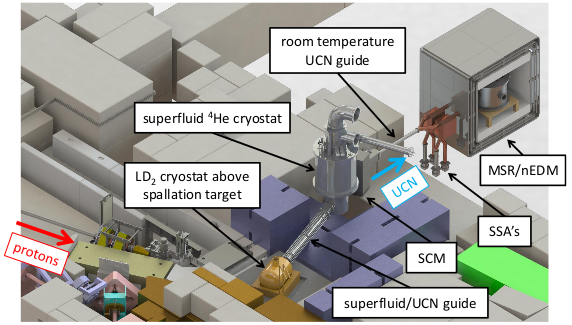
\includegraphics[width=1.0\textwidth]{edmtriumf.png}
  \caption[Conceptual design of TUCAN's future nEDM
  facility]{Conceptual design of the proposed UCN source and nEDM
    experiment. Protons strike a tungsten spallation target. Neutrons
    are moderated in the LD$_2$ cryostat and become UCN in a
    superfluid $^4$He bottle, which is cooled by another cryostat
    located farther downstream. UCN pass through guides and the
    superconducting magnet~(SCM) to reach the nEDM experiment located
    within a magnetically shielded room~(MSR). Simultaneous spin
    analyzers~(SSA’s) detect the UCN at the end of each nEDM
    experimental cycle.  }
  \label{fig:triumfEDM}
\end{figure}

%A schematic overview of the proposed UCN source upgrades, and the nEDM
%experiment is presented in Fig.~\ref{fig:triumfEDM}.
A brief description of the main components of the future nEDM aparatus
at TRIUMF is presented below.

\subsection{New UCN Source\label{sec:newUCNsource}}


The future nEDM experiment at TRIUMF will use a new upgraded UCN
source, which has quite some differences with the vertical UCN source
described in Chapter~\ref{chap:UCNattriumf}. A conceptual design of
our next generation UCN source is shown in
Fig.~\ref{fig:newUCNsource_2}. The upgrade source is referred to as
``the new horizontal source'', because the UCN exit in a
near-horizontal direction. When UCN exit the He-II into vacuum, they
gain a kinetic energy equivalent to the neutron optical potential of
18.5~neV. This corresponds to a height in Earth’s gravity field of
18.1~cm. Therefore near-horizontal extraction of UCN is a reasonable
development for He-II sources.


The moderators and the He-II cryostat are surrounded by shielding blocks
made of steel. Additionally, neutron absorbers made of borated
polyethylene~(PE) line the moderators and the UCN guide to reduce
activation of the steel blocks by thermal neutrons. Including a 10~cm
of steel shilding and 5~cm of borated polyethelene, can significantly
reduce the activation of the cryostat in cases with large shielding
penetrations.

The heavy-water moderator at room temperature should act as a thermal
pre-moderator for fast neutrons, reducing the required amount of cold
moderator and the heat load on the cold moderator and UCN
converter. Additionally, it should be placed around the cold moderator
to reflect thermal neutrons back into it. Additional graphite blocks
should serve as removable reflectors. The spallation target should be
covered with a layer of lead, which has a low neutron-absorption cross
section and shields the cold moderator and converter from $\gamma$
radiation.

The purpose of the cold moderator is to produce the maximum number of
1~meV neutrons, with the minimum number of neutron captures in the
material. Minimizing the neutron captures is important to prevent
production of gamma rays which would heat the He-II in the UCN
production volume, as well as to minimize neutron loss (for this
reason, deuterated materials are preferable). Higher energy $>$~1~meV
neutrons can also be used, since multiphonon excitations in the
superfluid can potentially produce UCN~\cite{Schmidt2009,
  Korobkina2002}. The new UCN source uses an LD$_2$ cryostat to
produce cold neutrons during the experiment, as opposed to the solid
D$_2$O in the vertical source. LD$_2$ increases the UCN production by
factors, and reduces the uncertainty in the UCN source performance.



The UCN production and detection of the new source are estimated in
details based on an Monte Carlo N-Particle~(MCNP) model of the source,
an analytical model of UCN production based on
Ref.~\cite{Korobkina2002}, and UCN transport simulations based on
Ref.~\cite{schreyer2017pentrack} including losses on walls and within
the He-II and the vapor pressure above it.  The simulations indicate
that when driven by a 40~$\mu$A proton beam, the source will produce
$2\times 10^7$~UCN/s, with beam heating to the He-II $<~10$~W, a
design goal for our refrigerator. At the end of target irradiation,
$3.4\times 10^8$~UCN would be in the source prior to opening the
room-temperature valve to the nEDM experiment.  The simulations also
include transport into the nEDM experiment. A total of
$6.5 \times 10^6$~UCN would be loaded into the EDM measurement cells
prior to initiating the Ramsey cycle. Using reasonable values for
lifetimes and spin-coherence times of the UCN, this corresponds to a
statistical determination of the nEDM of
$\sigma(d_n) = 3\times 10^{-25}$~e$\cdot$cm per cycle. Using
reasonable assumptions for the running time available per day, a
statistical determination of $\sigma(d_n) = 10^{-27}$~e$\cdot$cm would
be achieved in 400 days.

The new UCN source will have several key improvements. Foremost of these
is improved heat exchanger design and improved cooling
efficiency. Also to be improved are the internal neutron guides. We
plan to use an Al-Be alloy bottle presenting a lower heat load to the
He-II. Gamma and beta heating from the Al bottle walls is presently
projected to dominate the heat load to the superfluid. Extraction of
UCN from the source would be improved by the near-horizontal
extraction.

%A room-temperature Al window within a superconducting
%magnet will provide vacuum separation. The Al window will prevent
%contaminants from entering the He-II, while the superconducting magnet
%will accelerate high-field-seeking UCN through the window, resulting
%in highly polarized UCN after extraction.

%\begin{figure}[h!]
%  \centering
%  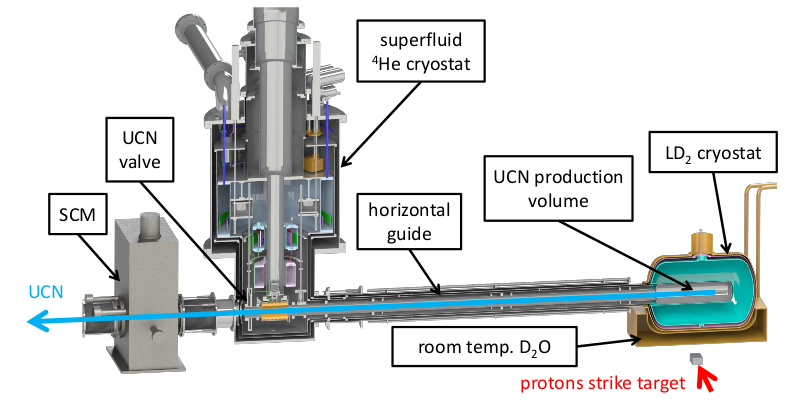
\includegraphics[width=1.0\textwidth]{newUCNsource.png}
%  \caption{The 3D model of the proposed UCN source and the LD$_2$
%    cryostat. Protons strike a tungsten spallation target liberating
%    neutrons, which are moderated in surrounding volumes of graphite
%    (not shown), D$_2$O, and LD$_2$. Neutrons are downscattered in the
%    UCN production volume containing superfluid $^4$He. They are
%    bottled within a horizontal guide up to a UCN valve. When the
%    valve is opened, UCN are transported to room temperature UCN
%    guides.}
%  \label{fig:newUCNsource}
%\end{figure}

\begin{figure}[h!]
  \centering
  \includegraphics[width=1.0\textwidth]{newUCNsource_2.png}
  \caption[Conceptual design of TUCAN's new UCN source]{Conceptual
    design of the next generation UCN source planned for
    TRIUMF. Neutrons are liberated by proton-induced spallation in a
    target located beneath the He-II, and LD$_2$ and D$_2$O
    moderators. Neutrons are reflected and moderated in surrounding
    materials, then enter superfluid $^4$He~(He-II), where they are
    downscattered. Cooling for the superfluid is provided by heat
    exchanger within the He-II cryostat. UCN created in the He-II are
    transported out through the heat exchanger passing through the
    He-II surface into vacuum in a vertical rise, and to the
    experiment which is conducted at room temperature.}
  \label{fig:newUCNsource_2}
\end{figure}

\subsection{UCN Handling and Transport}

Efficient transport of polarized UCN is one of the major requirements
for the nEDM measurement. This efficiency depends mainly
on three parameters as described below:

The first parameter is the capacity of the guide walls to contain the
UCN. UCN have a large wavelength compared to the lattice constants in
solid matter~(50 to 130~nm compared to 0.3~nm). Therefore, during a
scattering process, a UCN interacts with hundreds of nuclei. The mean
nuclear potential experienced during the scattering~(Fermi potential)
depends on the material. In order to store UCN, the Fermi potential
must be as high as possible.

The second parameter is the roughness of the surface. Indeed,
transportation is more efficient if the roughness is low. Then, the
probability of having a specular reflection is increased. Empirically,
a roughnesses should be lower than the UCN wavelength.

The last parameter is related to the polarization. UCN can be
depolarized during a collision due to different processes.
%such as spin incoherent nuclear scattering, paramagnetic scattering or
%large magnetic field gradients.
When selecting materials for UCN components, the mean depolarization
rate per bounce should be as small as possible.
\begin{figure}[h!]
  \centering
  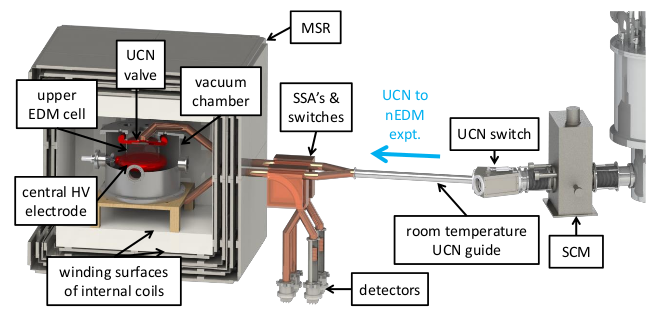
\includegraphics[width=1.0\textwidth]{UCNdelivery.png}
  \caption[3D model of TUCAN's future UCN delivery for the nEDM
  measurement]{A 3D model of the UCN delivery and the future nEDM
    experiment at TRIUMF. UCN exit the source by passing through the
    SCM spin polarizer, and UCN switch and detector system, where they
    then enter the proposed nEDM experiment. UCN are loaded into the
    measurement cells within a MSR/coil system. At the end of the
    measurement cycle, UCN are counted by simultaneous spin
    analyzers~(SSA’s) including detectors. An ambient magnetic
    compensation system, and thermally controlled room, will surround
    the nEDM apparatus~(not shown). For scale, the innermost layer of
    the MSR is a 1.8~m side-length cube.}
  \label{fig:UCNdelivery}
\end{figure}



The main task of the UCN handling parts is to transport a large
phase-space fraction of the UCN most efficiently to achieve the
highest statistical sensitivity in the experiment as possible.

The parts that come in contact with UCN on the way from the UCN source
to the EDM experiment, and the UCN detectors, constitute the neutron
handling hardware: UCN guides, valves, switches and simultaneous spin
analzer~(SSA) system. Fig.~\ref{fig:UCNdelivery} shows the neutron
handling parts for the future nEDM experiment at TRIUMF.  UCN exiting the
source are polarized by the SCM, and then enter the nEDM experiment.

Suitable guides and valves have optimized geometries: wall materials
with large Fermi potentials, low upscattering and absorption cross
sections for neutrons, and low roughness and depolarization. The plan is
to use Be for the UCN production volume, and NiMo coatings for most
other surfaces, on glass and Cu substrates, where non-magnetic
polarization preserving guides are required.  

UCN spins will be measured by two separate simultaneous spin analyzer
(SSA) systems (one for each cell). Its configuration allows
simultaneous counting of both UCN spin states, and maximizes the
visibility of the Ramsey fringes and counting efficiency.  The UCN
switches load the UCN into the nEDM experiment, and divert UCN exiting
the experiment into the detectors.  A prototype detector, based on
scintillating lithium glass, and capable of handling the highest rates
of UCN expected with the TRIUMF source has been developed and tested
in the highest rate UCN beam available at
PSI~\cite{jamieson2017characterization}~(See
Chapter~\ref{chap:UCNattriumf}).
%This detector is based on the detector used
%in the PSI UCN experiments~\cite{Ban2009}.



%The cold neutron guides contain liquid helium (shown in purple in
%Fig.~\ref{fig:UCNhandling}) at a temperature of less than 1~K. A cold
%UCN gate valve partitions this volume. Upstream of it, the neutrons
%are stored/accumulated while the proton beam irradiates the
%target. Three aluminum foils constitute the end of the 1~K neutron
%guide section, sitting inside a 3.5~T superconducting magnet, the UCN
%polarizer. A transition region of guides bridges between temperatures
%from 100~K to room temperature, which is the temperature of all
%downstream neutron handling equipment.

%At TRIUMF, the room temperature UCN guide will be split between the
%EDM experiment and the second experiment port via a Y-switch. Towards
%the EDM cell(s), the UCNs pass another UCN switch (aka. rotary valve
%or EDM detector switch) which can either guide neutrons from the
%source to the EDM cell or from the EDM cell to the UCN detectors. Each
%EDM cell itself is closed by a plug (or door valve) to store the
%neutrons during the Ramsey cycle. The vertical section of the UCN
%guides towards the UCN detectors contains spin flippers and spin
%analyzers and the UCN detectors at the bottom.

%To systematically check all possible alignments of electric field,
%magnetic field and neutron spin in the EDM experiment, a spin flipper
%can be added to the UCN guide system after the Y-switch and before it
%is possibly split to serve the two EDM cells. In this way, both
%neutron spin states can be loaded into the experiment. The spin
%analyzer uses a magnetic potential of 60 neV/T to analyze the neutron
%spin direction, deter- mining whether it’s spin is aligned~(low field
%seekers), or anti-aligned~(high field seekers) with the analyzer
%magnetic field.





\subsection{Magnetic Fields in the nEDM Experiment}
To achieve the desired nEDM sensitivity of ~$10^{-27}$~e$\cdot$cm, an
extremely stable and homogeneuos $B_0$ magnetic field is required.
The magnetic stability upper limit for TUCAN's nEDM measurement is
1~pT and the magnetic homogeneity upper limit is 1~nT/m.
%beyond which a comagnetometer must be
%used to correct the field to the $\sim$∼10~fT level.
Because of the challenges to achieve this level of magnetic stability,
a $^{199}$Hg co-magnetometer will be used to correct for the $B_0$
field fluctuations. To achieve these specifications, both active and
passive shielding will be utilized to nullify the uncontrolled and
time-varying external fields. The desired internal magnetic field will
be generated by using uniform and shim
coils. Fig.~\ref{fig:magneticscheme} shows the schematic drawing of
the magnetic components of the TUCAN nEDM experiment. Each magnetic
component is explained below.

\begin{figure}[h!]
  \centering
  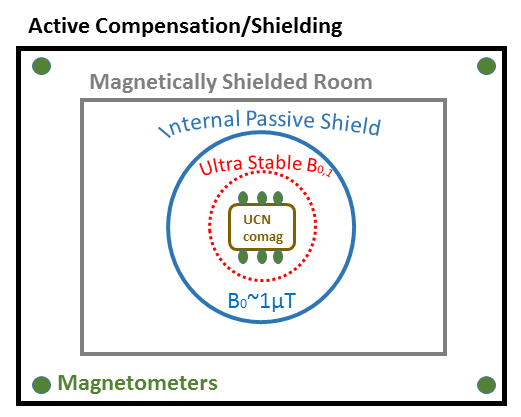
\includegraphics[width=0.7\textwidth]{magneticscheme.png}
  \caption[Schematic of TUCAN's nEDM magnetics components]{Schematic
    drawing for the TUCAN nEDM magnetics. From outside in: The active
    compensation system followed by several layers of magnetically
    shielded room and passive shields nullify the environmental
    magnetic field. The magnetometers inside the active shielding
    monitor the changes in the magnetic field internal to that
    region. The internal coil system~($B_0$ and $B_1$ coils) generate
    the magnetic fields for the Ramsey cycle. The UCN and the
    co-magnetometers are internal to the coils.  }
  \label{fig:magneticscheme}
\end{figure}



\subsubsection{Active Shielding}

The magnetic environment at the location of the planned nEDM
experiment at TRIUMF is dominated by a 400~$\mu$T static field due to
the main cyclotron at TRIUMF, with 1 to 100~nT fluctuations due to the
other external magnetic sources such as the electrical equipment or
the displacement of large magnetic objects~(e.g., vehicle traffic).

The TUCAN's plan is to reduce the static field to less than 50~$\mu$T
using dedicated compensation coils and constant-current supplies, with
a readily achievable steability of $10^{-3}$, and to reduce the
remaining static field and fluctuations by up to a factor of 100
through a separate set of compensation coils and current supplies,
using fluxgate magnetometers for magnetic feedback. The fluxgate
sensors will be placed in the region between the compensation coils
and the passive shields as shown in Fig.~\ref{fig:magneticscheme}.  A
prototype active compensation system has been built at the University
of Winnipeg based on Refs.~\cite{beatrice,afach2014dynamic}. The
system employs a set of coils centered around a cylindrical passive
magnetic shield system, using four 3-axis fluxgates for feedback~(see
Fig.~\ref{fig:prototype_active}). Overall, the active shielding system
should be able to reduce the net background magnetic field to the
level of tens of nT over the volume of the nEDM cell.


\begin{figure}[h!]
  \centering
  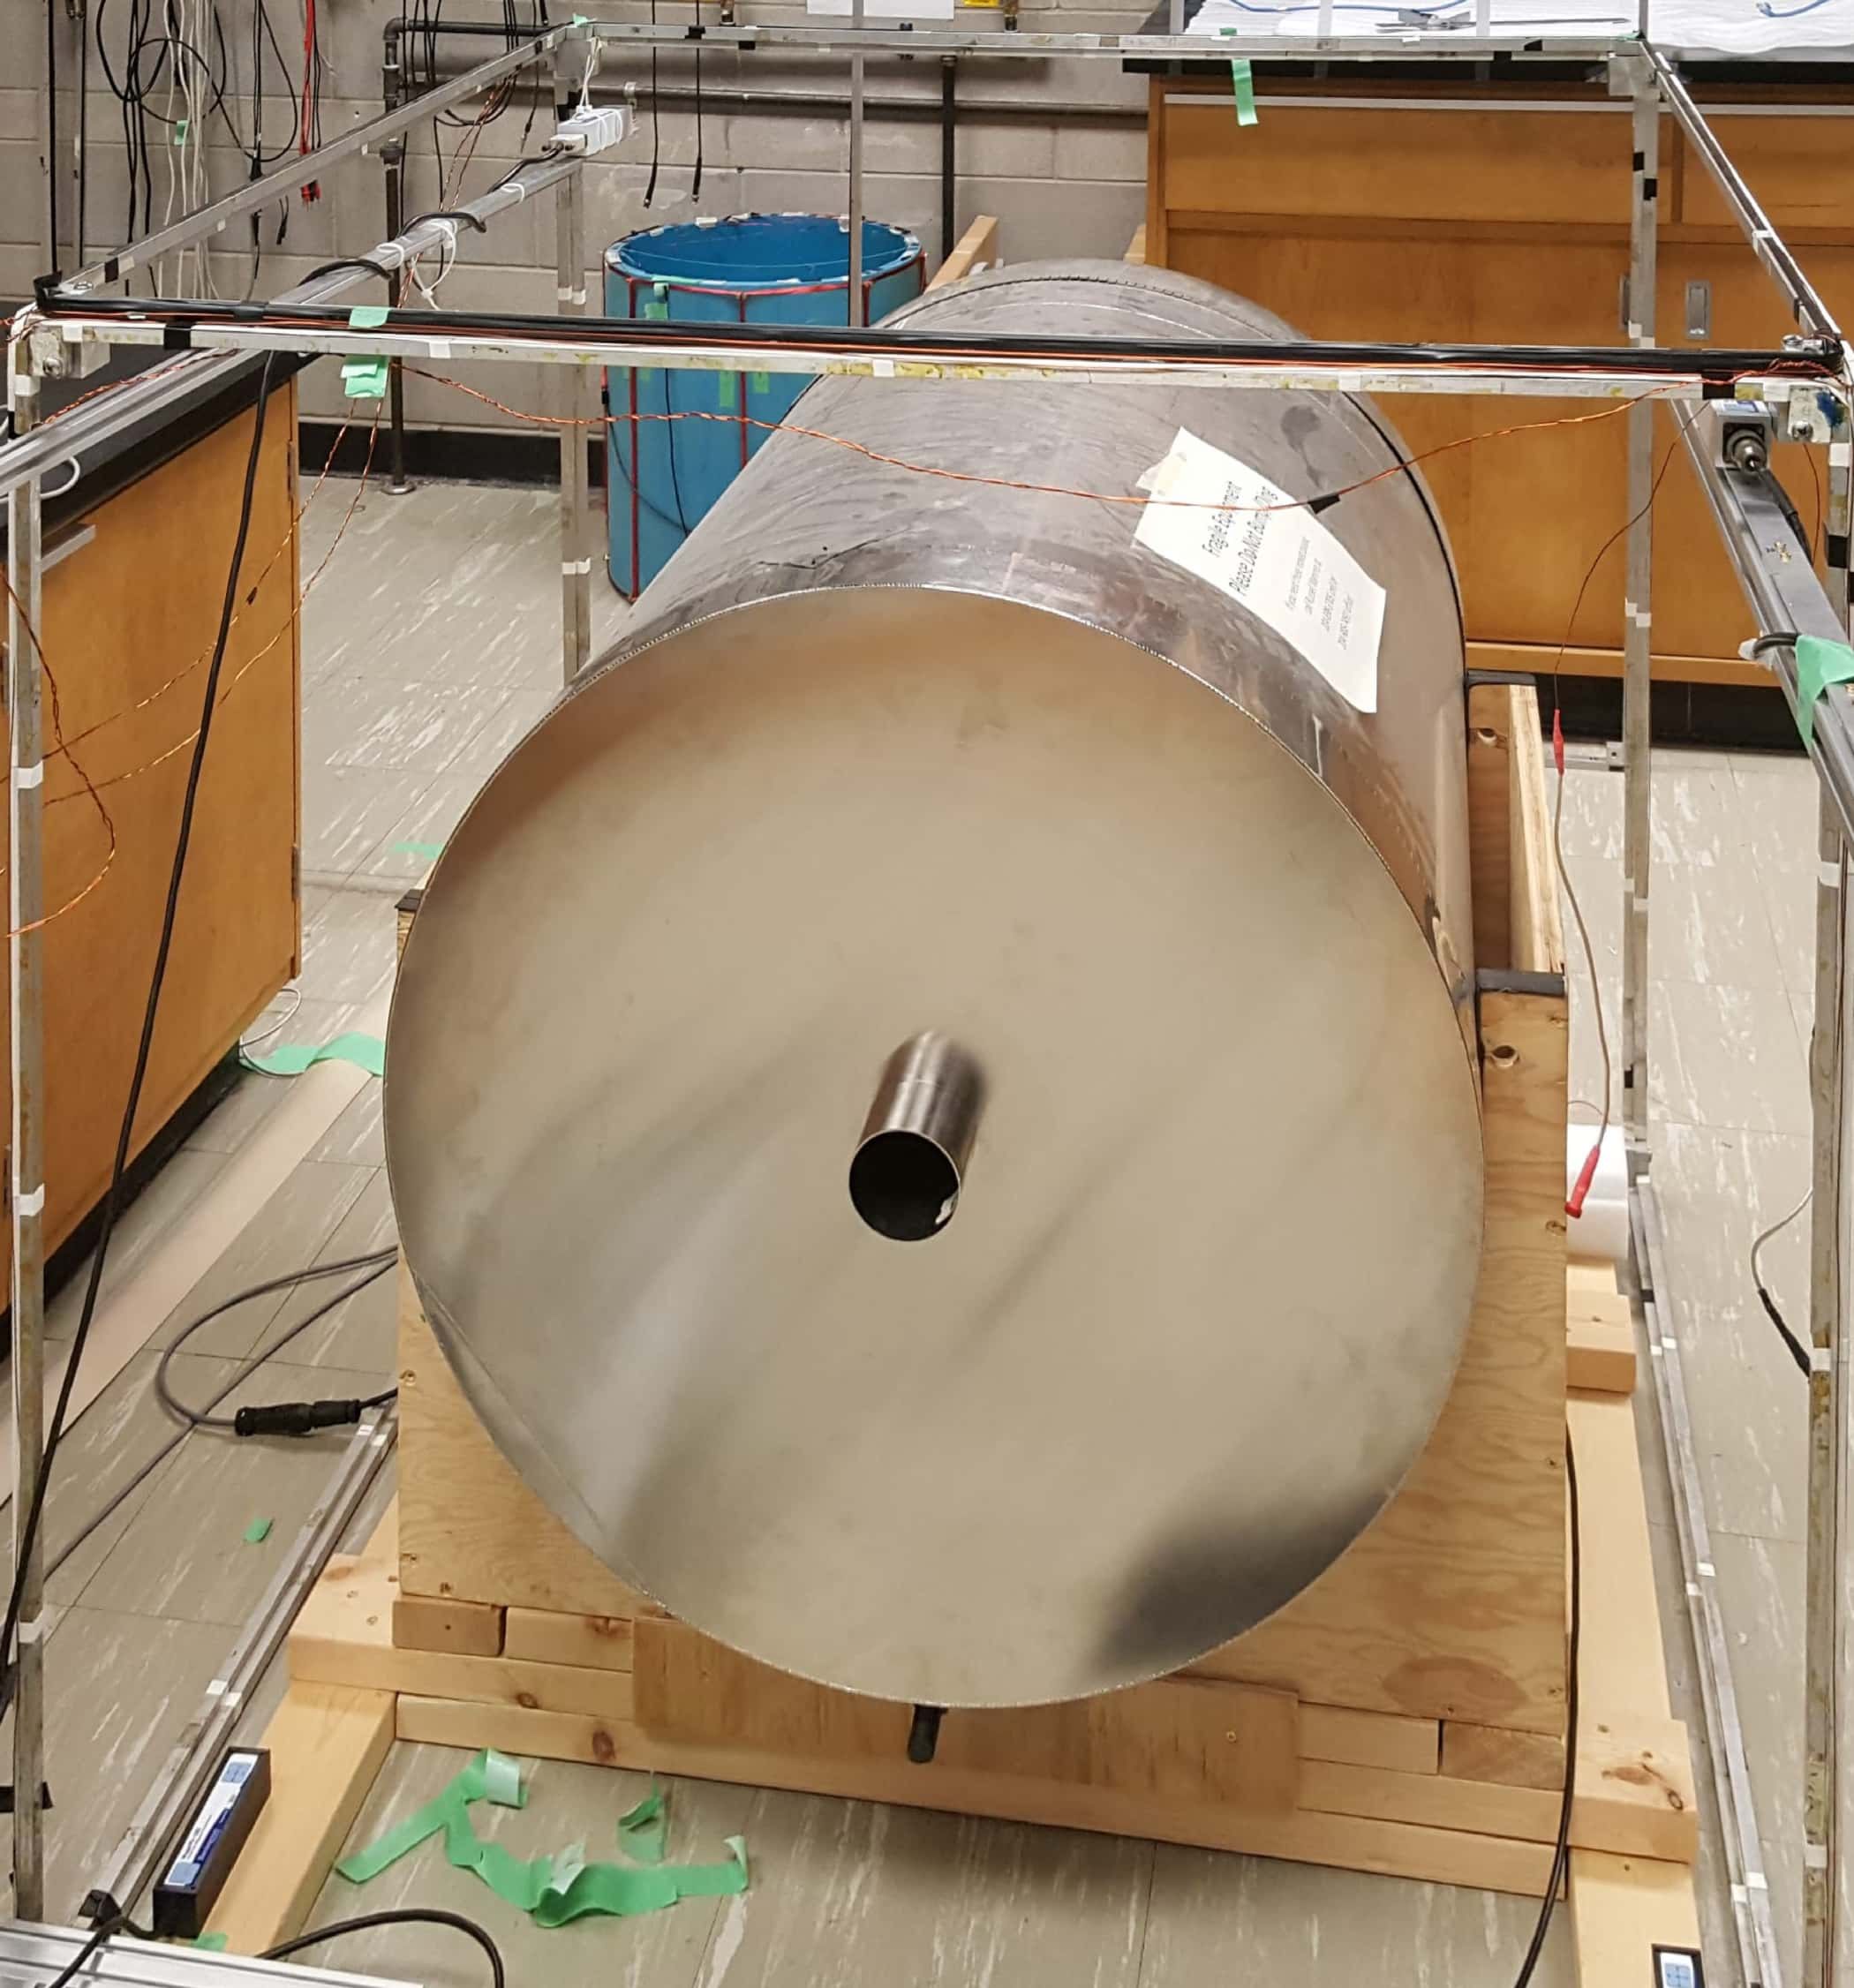
\includegraphics[width=0.7\textwidth]{active_prototype.jpg}
  \caption[TUCAN's prototype active compensation system]{The prototype
    active compensation system at the University of Winnipeg.}
  \label{fig:prototype_active}
\end{figure}

\subsubsection{Passive Shielding}


Passive magnetic shielding system is generally composed of a multi-layer
shield formed from thin shells of material with high magnetic
permeability~(e.g., mu-metal).  The outer layers of the shield are
normally cylindrical~\cite{serebrov2014new,baker2011search} or form
the walls of a magnetically shielded
room~\cite{altarev2014magnetically,altarev2015minimizing}.  The
innermost magnetic shield is normally a specially shaped shield, where
the design of the coil in relation to the shield is carefully taken
into account to achieve adequate
homogeneity~\cite{Baker2006,Kirch_talk,altarev2012next}. Fig.~\ref{fig:prototype_shields}
shows a picture of a prototype passive shield at the University of
Winnipeg, which is in support of the precision magnetic field research
for the future nEDM experiment to be conducted at TRIUMF.  The shield
system is a four-layer mu-metal shield formed from nested
right-circular cylindrical shells with endcaps.  The inner radius of
the innermost shield is 18.44~cm, equal to its half-length. The radii
and half-lengths of the progressively larger outer shields increase
geometrically by a factor of 1.27.  Each cylinder has two endcaps
which possess a 7.5~cm diameter central hole.  A stove-pipe of length
5.5~cm is placed on each hole, was designed to minimize leakage of
external fields into the progressively shielded inner volumes.  The
design is similar to another smaller prototype shield discussed in
Ref.~\cite{martin2015large}.

\begin{figure}[h!]
  \centering
  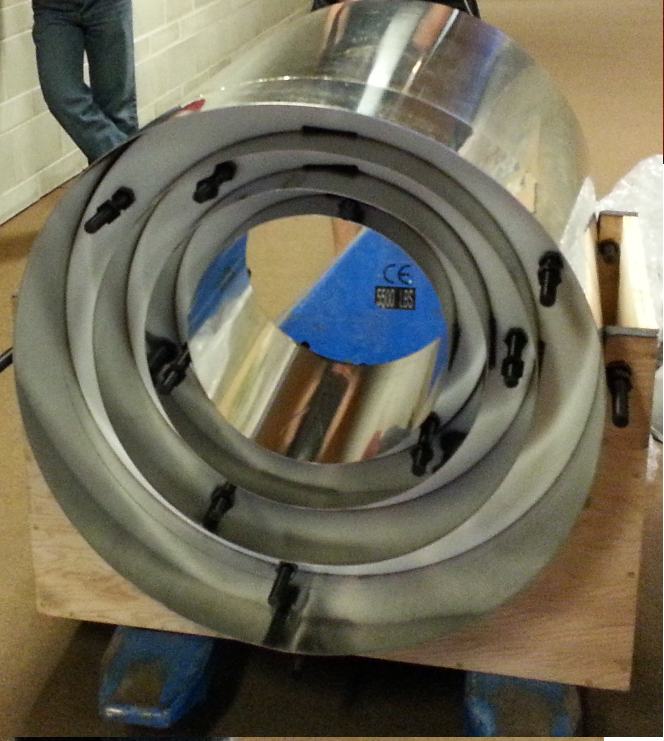
\includegraphics[width=0.6\textwidth]{prototype_shields.png}
  \caption[TUCAN's prototype passive shielding]{Three layers of the
    prototype passive magnetic shield at the University of
    Winnipeg. The 4th layer is not shown in this picture.}
  \label{fig:prototype_shields}
\end{figure}


The TUCAN's passive shielding system will reduce the magnetic field to
the pT level. It will be a two-stage system: (1) a magnetically
shielded room~(MSR) with (2) a set of smaller shields that fit inside
the room and surround the nEDM apparatus.

A magnetically shielded room~(MSR) with quasi-static
shielding factor of $\sim$~100,000 is sufficient to reduce the magnetic
fluctuations to the $\sim$~pT level. A four-layer MSR with an inner
cubic space of side-length 1.8~m and outer side-length 2.8~m produces
this shielding factor, with mu-metal wall thicknesses 2~mm, 6~mm,
4~mm, 4~mm (inner to outer), equally spaced.


The innermost layer of the ineternal passive shields also serves as a
return yoke for the magnetic flux generated by the internal coils for
the shield-coupled coil designs. A degaussing~(idealization) system
will be used to stabilize the shields. A combined DC shielding factor
of the order of $10^6$ is expected.


In principle, by utilizing both active and passive shielding, the
magnetic field from external sources will be reduced to the level of
tens of fT over the volume of the nEDM cell.  There are two prototype
four-layer mu-metal passive shields at the University of Winnipeg. The
shields are used to facilitate a variety of magnetic field R\&D. In
addition, there are three small witness cylinders which are made of
the same material and annealed in the same oven as the large passive
shields. The design principles behind the small shield, shielding
factor measurements, and comparison to simulation are described in
Ref.~\cite{martin2015large}.  The witness cylinders are used to
evaluate the temperature dependence of the shield material properties,
which could be an important consideration for internal field
stability~(see chapter~\ref{chap:muofT}).


\subsubsection{Internal Coils}
For internal coils, self-shielded $B_0$ coils and shim coils are
considered surrounding the nEDM cells, since they provide immunity
from the field perterbations induced by changes in the magnetic
permeability of the passive shields arising from temperature
fluctuations~(see chapter~\ref{chap:muofT}).  High-precision current
supplies ($\sim$~1~ppm) will be used to drive all internal coils,
regardless of design. AC coils will apply $\pi/2$ pulses for the UCN
and comagnetometer species, to initiate free spin precession.

%\textbf{also add field mapping and magnetometers???}


\subsection{ EDM Cells and High Voltage System}
The nEDM measurement volume consists of two storage cells to enable
simultaneous measurements with both up and down orientations of the
electric field~(see Fig.~\ref{fig:HVcell}). The storage cells will be
housed inside a non-magnetic vacuum chamber, providing insulating
vacuum for the high voltage applied to the central electrode which
separates the two cells. The cells are separated by a cylindrical
wall of dielectric insulator. The insulator must have a large
dielectric strength and low permittivity. An electric field of
12~kV/cm will be created between the electrodes with minimal leakage
current~($<$~10~pA). The optical readout of the comagnetometer
requires UV-transparent windows in the insulating side wall. The use
of two cells with a central electrode allows first-order compensation
of magnetic field drifts and a measurement of the magnetic field
gradient.

\begin{figure}[h!]
  \centering
  \includegraphics[width=1.0\textwidth]{EDMcell.png}
  \caption[3D drawing of TUCAN's double EDM cell]{3D drawing of the
    double EDM cell with vacuum chamber and UCN guides. All parts are
    labeled in the figure.}
  \label{fig:HVcell}
\end{figure}



\subsection{Comagnetometry}
A problem in a typical nEDM experiment is that, if the magnetic field
$B_0$ drifts over the course of the measurement period, it degrades
the statistical precision with which $d_n$ can be determined.  If the
magnetic field over one measurement cycle is determined to
$\delta B_0=10$~fT, it implies an additional statistical error of
$\delta d_n\sim 10^{-26}$~e$\cdot$cm~(assuming an electric field of
$E=10$~kV/cm, which is reasonable for a neutron EDM experiment). Over
100 days of averaging, this would make a
$\delta d_n\sim 10^{-27}$~e$\cdot$cm measurement possible.
Unfortunately, the magnetic field in the experiment is never stable to
this level.  For this reason, experiments use a comagnetometer and/or
surrounding atomic magnetometers to measure and correct the magnetic
field to this
level~\cite{Baker2006,brys2005magnetic,afach2014dynamic}. Drifts of
1-10~pT in $B_0$ may be corrected using the comagnetometer technique,
setting a goal magnetic stability for the $B_0$ field generation
system in a typical nEDM experiment.



A false nEDM signal may arise due to a combination of a magnetic field
gradient $\partial {B_z}/\partial z$, and motion in the electric field
when species~(neutrons and $^{199}$ Hg atoms) are confined in the
measurement cells. Comagnetometry offers the only way to correct for
false EDMs caused by leakage currents.  Each $^{199}$Hg atom is
polarized using optical pumping techniques. Polarized atoms are
introduced into the nEDM cell at the same time as UCN, and the
spin-precession frequencies of them are measured simultaneously. The
atoms are expected to have smaller EDMs than the neutrons, and so
their precession frequencies may be used to normalize magnetic field
drifts.  The design of the $^{199}$Hg comagnetometer will be similar
to that employed in the previous ILL
experiment~\cite{Baker2006,Griffith2009}.

%\section{ nEDM Measurement Worldwide}



%%%%%%%%%%%%%%%%%%%%%%%%%%%%%%%%%%%%%%%%%%%%%%%%%
%% repeating myself
%%%%%%%%%%%%%%%%%%%%%%%%%%%%%%%%%%%%%%%%%%%%%%%%%
%\subsection{UCN Handling and Transport}
%Fig.~\ref{fig:UCNdelivery} shows the UCN transport to the EDM cell.
%UCN will be transported out of the source by specular reflection via
%guides with special coatings compatible with UCN transport and
%polarization. Special coatings such as NiMo, NiP and DLC are top
%candidates because of their high Fermi potential , small absorption
%and inelastic upscattering, and good specularity.  A superconducting
%magnet (SCM) accelerates polarized UCN through barrier foils to a
%vacuum volume at room temperature. The UCN are then transported to the
%nEDM experiment by additional guides.



%\begin{figure}[h!]
%  \centering
%  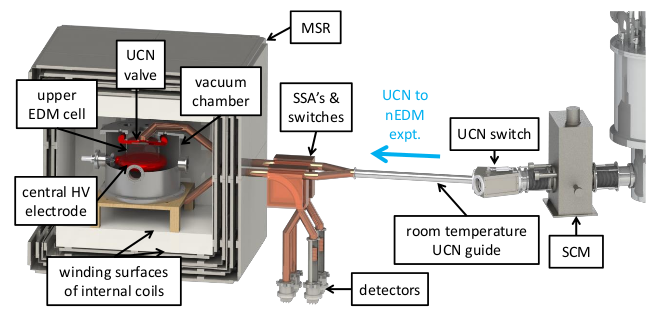
\includegraphics[width=1.0\textwidth]{UCNdelivery.png}
%  \caption{UCN delivery and the nEDM experiment. UCN exit the source
%    by passing through the SCM spin polarizer and UCN switch and
%    detector system, where they then enter the proposed Phase 2 nEDM
%    experiment. UCN are loaded into the measurement cells within a
%    MSR/coil system. At the end of the measurement cycle, UCN are
%    counted by simultaneous spin analyzers (SSA’s) including
%    detectors. An ambient magnetic compensation system and thermally
%    controlled room which will surround the nEDM apparatus~(not
%    shown). For scale, the innermost layer of the MSR is a 1.8~m
%    side-length cube.}
%  \label{fig:UCNdelivery}
%\end{figure}



%\subsection{DAQ?}
%\begin{description}
%\item{An introduction about the long term nEDM effort at TRIUMF, what
% the plan is, when it will start (roughly). I guess I can probably
% get this information from some proposals. I am not sure how much
% detail should go here.}
  
%\item{How the EDM experiment is actually done, talk about different
%  components of the system. Here is where I talk about the Ramsey
%  cycle ...}
  
%\item{nEDM measurement systematic effects: This is where I talk about
%  the GPE and ... . Basically here is to kind of motivate that we need
%  to have stable magnetic fields and we need lots of neutrons.}
  
%\item{Introduction to the magnetic stability requirements at
%  TRIUMF. What I mean is that there is 400 $\mu$T background field at
%  TRIUMF. Hopefully we have a field map of the area soon(?).}
  
%\item{From ouside in: Magnetically shielded room, what is the status
%  of that, are we going to have it? when? How good is it going to be
%  compared to the other ones worldwide? Why is it designed that way?
%  What is the design? Drawings of it. General question: Some of these
%  are about things that will happen in the future and I have not
%  worked on them. Should they even go to my thesis? I feel I have to
%  say a little about this since my thesis is nEDM related and it is
%  part of it.}
  
%\item{Passive shieldings: Again same questions as above, motivate for
%  the next chapter}

  
%\item{Say what will be discussed in the two coming chapters}
  
%\item{what else?}
%\end{description}

%%%%%%%%%%%%%%%%%%%%%%%%%%%%%%%%%%%%%%%%%%%%%%%%%%%
%%% THE FOLLOWING IS THE \MU OF TEMP CHAPTER
%%%%%%%%%%%%%%%%%%%%%%%%%%%%%%%%%%%%%%%%%%%%%%%%%%%

\chapter{Temperature Dependence of Magnetic Permeability\label{chap:muofT}}


\section{Introduction}

The next generation of neutron electric dipole moment (nEDM)
experiments aim to measure the nEDM $d_n$ with proposed precision
$\delta d_n\lesssim
10^{-27}~e\cdot$cm~\cite{serebrov2014new,serebrov2011supersource,Kirch_talk,baker2011search,altarev2012next,golub1994neutron,ito2007plans,picker2017minuscule}.
In the previous best experiment \cite{baker2006,Pendlebury2015} which
discovered $d_n<3.0\times 10^{-26}~e\cdot$cm (90\% C.L), effects
related to magnetic field homogeneity and instability were found to
dominate the systematic error.  A detailed understanding of passive
and active magnetic shielding, magnetic field generation within
shielded volumes, and precision magnetometry is expected to be crucial
to achieve the systematic error goals for the next generation of
experiments.  Much of the research and development efforts for these
experiments are focused on careful design and testing of various
magnetic shield geometries with precision
magnetometers~\cite{brys2005magnetic,afach2014dynamic,altarev2014magnetically,Sturm_thesis,patton2014all}.

In nEDM experiments, the spin-precession frequency $\nu$ of neutrons
placed in static magnetic $B_0$ and electric $E$ fields is measured.
The measured frequencies for parallel $\nu_+$ and antiparallel $\nu_-$
relative orientations of the fields is sensitive to the neutron
electric dipole moment $d_n$
\begin{equation}
h\nu_\pm=2\mu_nB_0\pm 2d_nE
\end{equation}
where $\mu_n$ is the magnetic moment of the neutron.

A problem in these experiments is that if the magnetic field $B_0$
drifts over the course of the measurement period, it degrades the
statistical precision with which $d_n$ can be determined.  If the
magnetic field over one measurement cycle is determined to
$\delta B_0=10$~fT, it implies an additional statistical error of
$\delta d_n\sim 10^{-26}~e\cdot$cm (assuming an electric field of
$E=10$~kV/cm which is reasonable for a neutron EDM experiment).  Over
100 days of averaging, this would make a
$\delta d_n\sim 10^{-27}~e\cdot$cm measurement possible.
Unfortunately the magnetic field in the experiment is never stable to
this level.  For this reason, experiments use a comagnetometer and/or
surrounding atomic magnetometers to measure and correct the magnetic
field to this
level~\cite{baker2006,brys2005magnetic,afach2014dynamic}.  Drifts of
1-10~pT in $B_0$ may be corrected using the comagnetometer technique,
setting a goal magnetic stability for the $B_0$ field generation
system in a typical nEDM experiment.

In such experiments, typically $B_0=1~\mu$T is used to provide the
quantization axis for the ultracold neutrons.  The $B_0$ magnetic
field generation system typically includes a coil placed within a
passively magnetically shielded volume.  The passive magnetic shield
is generally composed of a multi-layer shield formed from thin shells
of material with high magnetic permeability (mu-metal).  The outer
layers of the shield are normally
cylindrical~\cite{serebrov2014new,baker2011search} or form the walls
of a magnetically shielded
room~\cite{altarev2014magnetically,altarev2015minimizing}.  The
innermost magnetic shield is normally a specially shaped shield, where
the design of the coil in relation to shield is carefully taken into
account to achieve adequate homogeneity
\cite{baker2006,Kirch_talk,altarev2012next}.

Mechanical and temperature changes of the passive magnetic
shielding~\cite{voigt2013,thiel2007demagnetizaion}, and the degaussing
procedure~\cite{thiel2007demagnetizaion,altarev2015minimizing,sun2016dynamic}
(also known as demagnetization, equilibration, or idealization),
affect the stability of the magnetic field within magnetically
shielded rooms.  Active stabilization of the background magnetic field
surrounding magnetically shielded rooms can also improve the internal
stability~\cite{voigt2013,afach2014dynamic,Franke_thesis}.  The
current supplied to the $B_0$ coil is generated by an ultra-stable
current source~\cite{brys2005magnetic}. The coil must also be
stabilized mechanically relative to the magnetic shielding.

One additional effect, which is the subject of this paper, relates to
the fact that the $B_0$ coil in most nEDM experiments is magnetically
coupled to the innermost magnetic shield.  If the magnetic properties
of the innermost magnetic shield change as a function of time, it then
results in a source of instability of $B_0$.  In the present work, we
estimate this effect and characterize one possible source of
instability: changes of the magnetic permeability $\mu$ of the
material with temperature.

While the sensitivity of magnetic alloys to temperature variations has
been characterized in the past~\cite{couderchon1982some,kruppvdm}, we
sought to make these measurements in regimes closer to the operating
parameters relevant to nEDM experiments.  For these alloys, it is also
known that the magnetic properties are set during the final annealing
process~\cite{gupta2007influence,bozorth1993ferromagnetism,kruppvdm}.
In this spirit we performed our measurements on ``witness'' cylinders,
which are small open-ended cylinders made of the same material and
annealed at the same time as other larger shields are being annealed.

The paper proceeds in the following fashion:
\begin{itemize}
\item The dependence of the internal field on magnetic permeability of
  the innermost shielding layer for a typical nEDM experiment geometry
  is estimated using a combination of analytical and finite element
  analysis techniques.  This sets a scale for the stability problem.
\item New measurements of the temperature dependence of the magnetic
  permeability are presented.  The measurements were done in two ways
  in order to study a variety of systematic effects that were
  encountered.
\item Finally, the results of the calculations and measurements are
  combined to provide a range of temperature sensitivities that takes
  into account sample-to-sample and measurement-to-measurement
  variations.
\end{itemize}




\section{Sensitivity of Internally Generated Field to Permeability of the Shield $B_0(\mu)$\label{sec:calculation}}

In nEDM experiments conducted in the past, the presence of a coil
inside the innermost passive shield turns the shield into a return
yoke, and generally results in an increase in the magnitude
of~$B_0$. The ratio of this field inside the coil in the presence of
the magnetic shield to that of the coil in free space is referred to
as the reaction factor~$C$, and can be calculated analytically for
spherical and infinite cylindrical
geometries~\cite{bidinosti2014passive,urankar1996design}. The key
issue of interest for this work is the dependence of the reaction
factor on the permeability $\mu$ of the innermost shield.  Although
this dependence can be rather weak, the constraints on~$B_0$ stability
are very stringent. As a result, even a small change in the magnetic
properties of the innermost shield can result in an unacceptably large
change in~$B_0$.


To illustrate, consider here the model of a sine-theta surface
current on a sphere of radius $a$, inside a spherical shell of inner
radius $R$, thickness $t$, and linear permeability $\mu$. The uniform
internal field generated by this ideal spherical coil is augmented by
the reaction factor in the presence of the shield, but is otherwise
left undistorted.  The general reaction factor for this model is given
by Eqn.~(38) in Ref.~\cite{bidinosti2014passive}.  In the high-$\mu$
limit, with $t\ll R$, the reaction factor can be approximated as
\begin{equation}
C 
 \simeq 1+ \frac{1}{2}\, \left( \frac{a}{R} \right)^{3} \left( 1- \frac{3}{2} \, \frac{R}{t} \, \frac{\mu_0}{\mu} \right) \, ,
 \label{Csphere}
\end{equation}
which highlights the dependence of $B_0$ on the relative permeability
$\mu_r=\mu/\mu_0$ of the shield.

Fig.~\ref{fig:Magnetic_Field} (upper) shows a plot of $B_0$ versus
$\mu_r$ for coil and shield dimensions similar to the ILL nEDM
experiment~\cite{Baker2006,knecht}: $a=0.53$~m, $R= 0.57$~m, and
$t=1.5$~mm.  In addition to analytic calculations, the results of two
axially symmetric simulations conducted using FEMM~\cite{femm} are
included to assess the effects of geometry and discretization of the
surface current. The differences are small, suggesting that the ideal
spherical model of Ref.~\cite{bidinosti2014passive} and the high-$\mu$
approximation of Eqn.~(\ref{Csphere}) provide valuable insight for the
design and analysis of shield-coupled coils.

%The dashed curve represents the
%results of an analytical calculation for a perfect spherical surface
%current.  For this calculation, a coil of radius 0.53~m inside a
%magnetic shield with inner radius $0.57$~m and thickness 1.5~mm were
%used.  The dimensions have been selected to be comparable to the
%dimensions of the ILL nEDM experiment
%geometry~\cite{baker,knecht}.

\begin{figure}[h!]
\begin{center}
   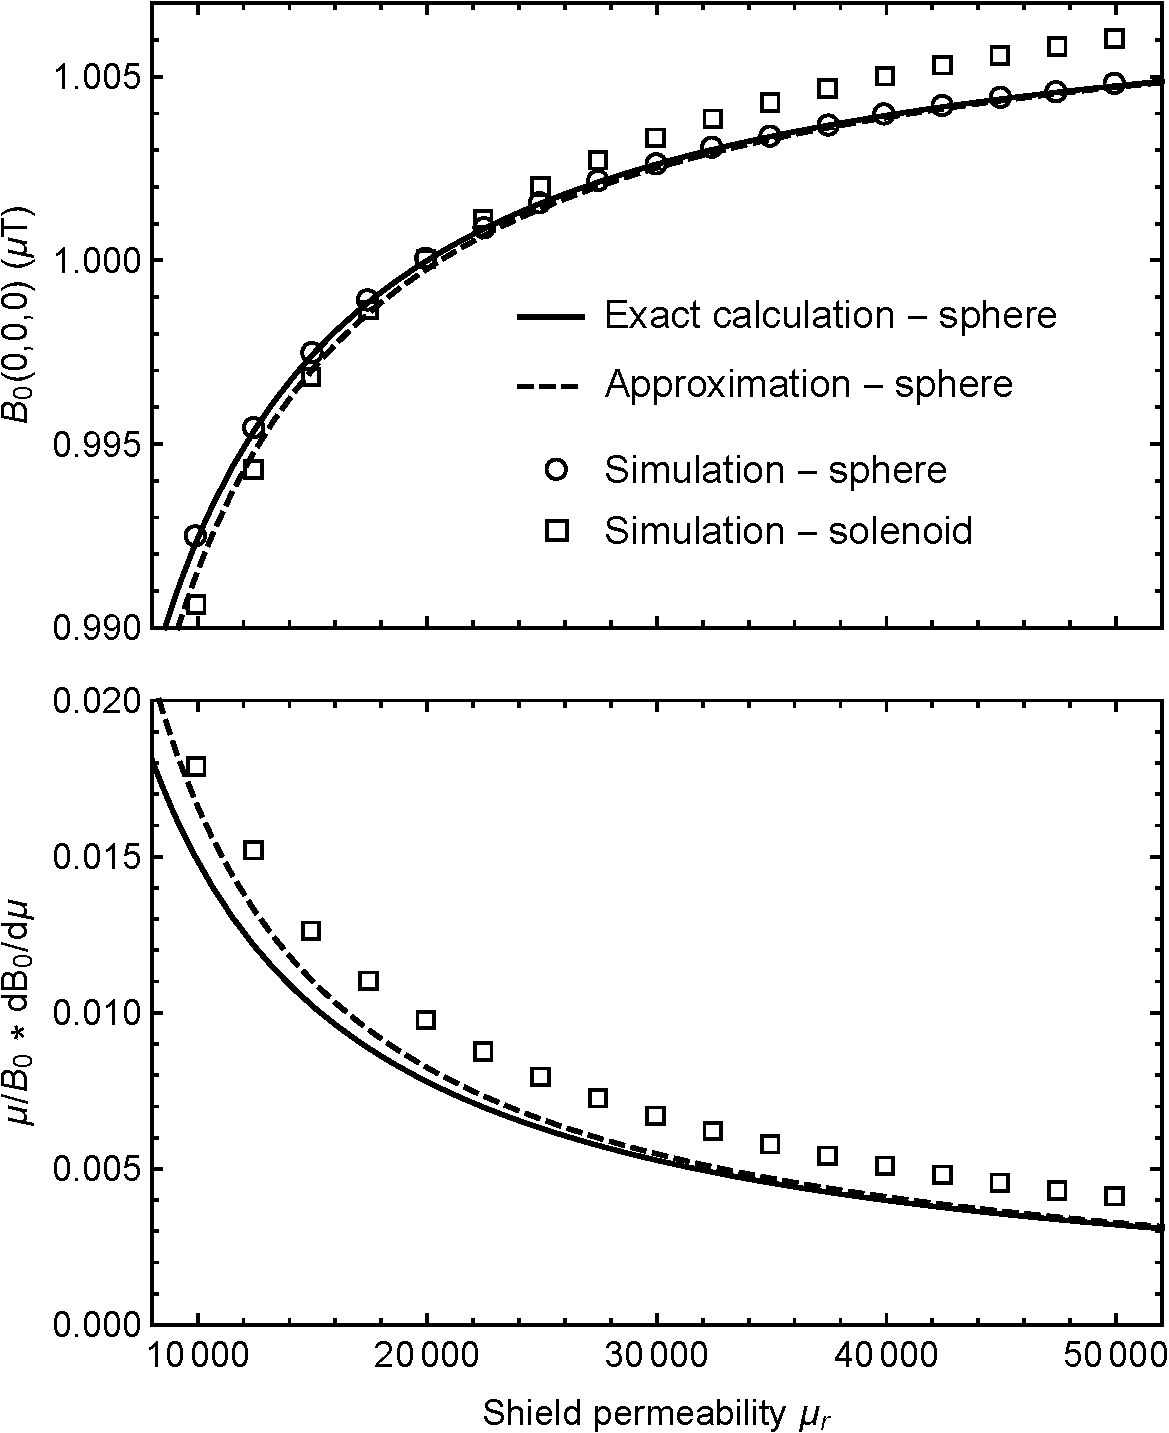
\includegraphics[width=0.7\textwidth]{Fig_combined-crop.pdf}
   \caption[Magnetic field $B_0$ and$\frac{\mu}{B_0}\frac{dB_0}{d\mu}$
   versus $\mu$]{Upper: Magnetic field at the coil center as a
     function of magnetic permeability of the surrounding magnetic
     shield for a geometry similar to the ILL nEDM experiment as
     discussed in the text.  Lower: $\frac{\mu}{B_0}\frac{dB_0}{d\mu}$
     vs.~permeability.  The solid curve is the exact calculation for
     the ideal spherical coil and shield from
     Ref.~\cite{bidinosti2014passive}; the dashed curve is the
     approximation of Eqn.~\ref{Csphere}. The circles and squares are
     the FEMM-based simulations for the spherical and solenoidal
     geometries with discrete currents.  Since the spherical
     simulation was in agreement with the calculation, it is omitted
     from the lower graph.  For the exact calculation and the two
     simulations, currents were chosen to give $B_0=1~\mu$T at
     $\mu_r=20,000$.}
    \label{fig:Magnetic_Field}
    \end{center}
\end{figure} 


In the first simulation, the same spherical geometry was used as for
the analytic calculations.  However, the surface current was
discretized to 50 individual current loops, inscribed onto a sphere,
and equally spaced vertically (i.e.~a discrete sine-theta coil). A
square wire profile of side length 1~mm was used. As shown in
Fig.~\ref{fig:Magnetic_Field}, this simulation gave excellent
agreement with the analytic calculations.  In the second simulation, a
solenoid coil and cylindrical shield (length/radius~=~2) were used
with the same dimensions as above.  Similarly, the coil was modelled
as 50 evenly spaced current loops, with the distance from an end loop
to the inner face of the shield endcap being half the inter-loop
spacing.  In the limit of tight-packing (i.e., a continuous surface
current) and infinite $\mu$, the image currents in the end caps of the
shield act as an infinite series of current loops, giving the ideal
uniform field of an infinitely long
solenoid~\cite{lambert1975magnetically,sumner1987calculation}. As shown in
Fig.~\ref{fig:Magnetic_Field}, the result is similar to the spherical
case, with differences of order one part per thousand and a somewhat
steeper slope of $B_0(\mu_r)$.

Fig.~\ref{fig:Magnetic_Field} (lower) shows the normalized slope
$\frac{\mu}{B_0}\frac{dB_0}{d\mu}$ of the curves from
Fig.~\ref{fig:Magnetic_Field} (upper).  In ancillary measurements of
shielding factors (discussed briefly in
Section~\ref{sec:previousmeasurement}), we found $\mu_r=20,000$ to
offer a reasonable description of the quasistatic shielding factor of
our shield.  Using this value as the magnetic permeability of our
shield material, Fig.~\ref{fig:Magnetic_Field} (lower) shows that
$\frac{\mu}{B_0}\frac{dB_0}{d\mu}$ varies by about 20\% (from 0.008 to
0.01) for the spherical vs.~solenoidal geometries.  We adopt the value
$\frac{\mu}{B_0}\frac{dB_0}{d\mu}=0.01$ as an estimate of this slope
in our discussions in Section~\ref{sec:relationship}, acknowledging
that the value depends on the coil and shield design.

For a high-$\mu$ innermost shield, the magnetic field lines emanating
from the coil all return through the shield.  This principle can be
used to estimate the magnetic field $B_m$ inside the shield material,
and in our studies gave good agreement with FEA-based simulations.
For the solenoidal geometry previously described and used for the
calculations in Fig.~\ref{fig:Magnetic_Field}, $B_m$ is largest in the
side walls of the solenoidal flux return, attaining a maximum value of
170~$\mu$T.  If we assume $\mu_r$=20,000, the $H_m$ field is
0.007~A/m.  Typically the shield is degaussed (idealized) with the
internal coil energized. After degaussing, $B_m$ must be approximately
the same, since essentially all flux returns through the shield.
However, the $H_m$ field may become significantly smaller because
after degaussing, it falls on the ideal magnetization curve in
$B_m-H_m$ space.  (For a discussion of the ideal magnetization curve,
refer to Ref.~\cite{bozorth1993ferromagnetism} and see
Fig.~\ref{fig:bh}.)  In principle, the $H_m$ field could be reduced by
an order of magnitude or more, depending on the steepness of the ideal
magnetization curve near the origin.  Thus $B_m=170~\mu$T and
$H_m<0.007$~A/m set a scale for the relevant values for nEDM
experiments.  Furthermore, the field in the nEDM measurement volume,
as well as in the magnetic shield, must be stable for periods of
typically hundreds of seconds (corresponding to frequencies
$<0.01$~Hz). This sets the relevant timescale for magnetic properties
most relevant to nEDM experiments.


\begin{figure}[h!]
  \centering
  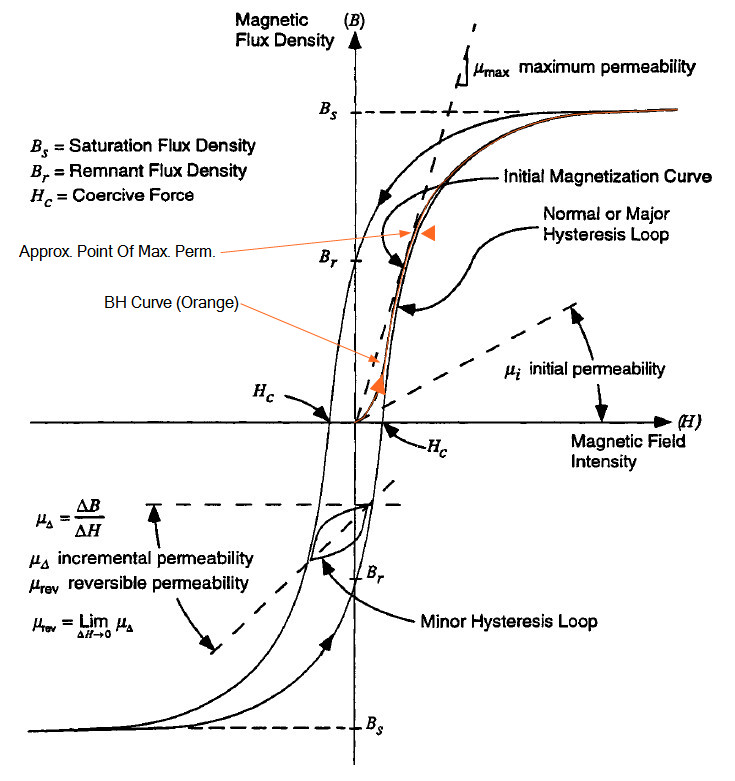
\includegraphics[width=0.8\textwidth]{bh.jpg}
  \caption[The hysteresis or $B-H$ curve]{The hysteresis or $B-H$
    curve. Some commonly used terminology is shown. $H_c$ or
    coercivity is a measure of the ability of the material to
    withstand external magnetic fields and is at $B=0$. Initial
    permeability or $\mu_i$ is the slope of the initial magnetization
    curve. The initial magnetization or idealization curve is
    achievable after degaussing the high $\mu$ material.}
  \label{fig:bh}
\end{figure}





\section{Measurements of $\mu(T)$\label{sec:tdep}}

\subsection{Previous Measurements and their Relationship to nEDM Experiments\label{sec:previousmeasurement}}

Previous measurements of the temperature dependence of the magnetic
properties of high-permeability alloys have been summarized in
Refs.~\cite{couderchon1982some,bozorth1993ferromagnetism,pfeifer1980soft}.  These
measurements are normally conducted using a sample of the material to
create a toroidal core, where a thin layer of the material is used in
order to avoid eddy-current and skin-depth
effects~\cite{pfeifer1980soft,kruppvdm}.  A value of $\mu$ is
determined by dividing the amplitude of the sensed $B_m$-field by the
amplitude of the driving AC $H_m$-field (similar to the method
described in Section~\ref{sec:transformer}).  Normally the frequency
of the $H_m$-field is 50 or 60~Hz.  The value of $\mu$ is then quoted
either at or near its maximum attainable value by adjusting the
amplitude of $H_m$.  Depending on the details of the $B_m-H_m$ curve
for the material in question, this normally means that $\mu$ is quoted
for the amplitude of $H_m$ being at or near the coercivity of the
material~\cite{couderchon1982some,kruppvdm}, resulting in large values
up to $\mu_r=4\times 10^5$.

It is well known that $\mu$ measured in this fashion for toroidal,
thin metal wound cores depends on the annealing process used for the
core.  There is a particularly strong dependence on the take-out or
tempering temperature after the high-temperature portion of the
annealing process has been
completed~\cite{pfeifer1980soft,kruppvdm,couderchon1982some}.  Such
studies normally suggest a take-out temperature of 490-500$^\circ$C.
This ensures that the large $\mu_r=4\times 10^{5}$ is furthermore
maximal at room temperature.  Slight variations around room
temperature, and assuming the take-out temperature is not controlled
to better than a degree, imply a scale of possible temperature
variation of $\mu$ of approximately
$\left|\frac{1}{\mu}\frac{d\mu}{dT}\right|\simeq 0.3$-1\%/K at room
temperature~\cite{couderchon1982some,kruppvdm}.

A challenge in applying these results to temperature stability of nEDM
experiments is that, when used as DC magnetic shielding, the
high-permeability alloys are usually operated for significantly
different parameters ($B_m$, $H_m$, and frequencies).

For example, when used in a shielding configuration, the effective
permeability is often measured to be typically $\mu_r=20,000$ rather
than $4\times 10^5$.  This arises in part because $H_m$ is well below
the DC coercivity.  As noted in Section~\ref{sec:calculation}, a more
appropriate $H_m$ for the innermost magnetic shield of an nEDM
experiment is $<0.007$~A/m, whereas the coercivity is
$H_c=0.4$~A/m~\cite{kruppvdm}.  The frequency dependence of the
measurements could also be an issue.  Typically, nEDM experiments are
concerned with slow drifts at $<0.01$~Hz timescales whereas the
previously reported $\mu(T)$ measurements are performed in an AC mode
at 50-60~Hz.


The goal of our experiments was to develop techniques to characterize
the material properties of our own magnetic shields post-annealing, in
regimes more relevant to nEDM experiments.


We created a prototype passive magnetic shield system in support of
this and other precision magnetic field research for the future nEDM
experiment to be conducted at TRIUMF.  The shield system is a
four-layer mu-metal shield formed from nested right-circular
cylindrical shells with endcaps.  The inner radius of the innermost
shield is 18.44~cm, equal to its half-length. The radii and
half-lengths of the progressively larger outer shields increase
geometrically by a factor of 1.27.  Each cylinder has two endcaps
which possess a 7.5~cm diameter central hole.  A stove-pipe of length
5.5~cm is placed on each hole was designed to minimize leakage of
external fields into the progressively shielded inner volumes.  The
design is similar to another smaller prototype shield discussed in
Ref.~\cite{martin2015large}.  The magnetic shielding factors of each of
the four cylindrical shells, and of various combinations of them, were
measured and found to be consistent with $\mu_r\sim 20,000$.
%-40,000$ for
%3.5~$\mu$T applied external axial and transverse fields at frequencies
%$<0.1$~Hz, where the uncertainty in $\mu_r$ comes a model uncertainty
%resulting from incomplete inclusion of the geometry.

In our studies of the material properties of these magnetic shields,
two different approaches to measure $\mu(T)$ were pursued.  Both
approaches involved experiments done using witness cylinders made of
the same material and annealed at the same time as the prototype
magnetic shields.  We therefore expect they have the same magnetic
properties as the larger prototype shields, and they have the
advantage of being smaller and easier to perform measurements with.

The two techniques employed to determine $\mu(T)$ were the following:
\begin{enumerate}
\item measuring the low-frequency AC axial magnetic shielding factor
  of the witness cylinder as a function of temperature, and
\item measuring the temperature-dependence of the slope of a minor B-H
  loop, using the witness cylinder as a transformer core, similar to
  previous measurements of the temperature dependence of $\mu$, but
  for parameters closer to those encountered in nEDM experiments.
\end{enumerate}
We now discuss the details and results of each technique.

% Axial shielding factor measurements Section moved to axial.tex


\subsection{Axial Shielding Factor Measurements\label{sec:axial}}

In these measurements, a witness cylinder was used as a magnetic
shield.  The shield was subjected to a low-frequency AC magnetic field
of $\sim 1$~Hz.  The amplitude of the shielded magnetic field $B_s$
was measured at the center of the witness cylinder using a fluxgate
magnetometer.  Changes in $B_s$ with temperature signify a dependence
of the permeability $\mu$ on temperature.  The relative slope of
$\mu(T)$ can then be calculated using
\begin{equation}
\frac{1}{\mu}\frac{d\mu}{dT}=-\frac{\frac{1}{B_s}\frac{dB_s}{dT}}{\frac{\mu}{B_s}\frac{dB_s}{d\mu}}.
\label{eqn:axial}
\end{equation}
The numerator was taken from the measurements described above. The
denominator was taken from finite-element simulations of the shielding
factor for this geometry as a function of $\mu$.

This measurement technique was sufficiently robust to extract the
temperature dependence of the shielding factor with some degree of
certainty. Possible drifts and temperature dependence of the fluxgate
magnetometer offset were mitigated by using an AC magnetic field.  Any
temperature coefficients in the rest of the instrumentation were
controlled by performing the same measurements with a copper
cylindrical shell with the similar size and shape as the mu-metal
witness cylinders in place of the mu-metal witness cylinder.

This technique is quite different than the usual transformer core
measurements conducted by other groups.  As shall be described, it
offers an advantage that considerably smaller $B_m$ and $H_m$ fields
can be accessed.  Measuring the temperature dependence of the
shielding factor is also considerably easier than measuring the
temperature dependence of the reaction factor, since the sensitivity
to changes in $\mu(T)$ is considerably larger in magnitude for the
shielding factor case where $\frac{\mu}{B_s}\frac{dB_s}{d\mu}\sim -1$
compared to the reaction factor case where
$\frac{\mu}{B_0}\frac{dB_0}{d\mu}\sim 0.01$.


\subsubsection{Experimental Apparatus for Axial Shielding Factor
  Measurements}

The witness cylinder was placed within a homogeneous AC magnetic
field. The field was created within the magnetically shielded volume
of the prototype magnetic shielding system (described previously in
Section~\ref{sec:previousmeasurement}) in order to provide a
controlled magnetic environment.  A short solenoid inside the
shielding system was used to produce the magnetic field. The solenoid
has 14 turns with 2.6~cm spacing between the wires.  The solenoid was
designed so that the field produced by the solenoid plus innermost
shield approximates that of an infinite solenoid.  The magnetic field
generated by the solenoid was typically 1~$\mu$T in amplitude.  The
solenoid current was varied sinusoidally at typically 1~Hz.

The witness cylinder was placed into this magnetic field generation
system as shown schematically in Fig.~\ref{fig:geometry}. The
cylinder was held in place by a wooden stand.

A Bartington fluxgate magnetometer Mag-03IEL70~\cite{bartman} (low
noise) measured the axial magnetic field at the center of the witness
cylinder.  The fluxgate was a ``flying lead'' model, meaning that each
axis was available on the end of a short electrical lead, separable
from the other axes.  One flying lead was placed in the center of the
witness cylinder, the axis of the fluxgate being aligned with that of
the witness cylinder.  The fluxgate was held in place rigidly by a
plastic mounting fixture, which was itself rigidly mounted to the
witness cylinder.

To increase the resolution of the measured signal from the fluxgate, a
Bartington Signal Conditioning Unit (SCU) was used with a low-pass
filter set to typically 10-100~Hz and a gain set to typically $>50$.
The signal from the SCU was demodulated by an SR830 lock-in
amplifier~\cite{lockin} providing the in-phase and out-of-phase
components of the signal.  The sinusoidal output of the lock-in
amplifier reference output itself was normally used to drive the
solenoid generating the magnetic field.  The time constant on the
lock-in was typically set to 3 seconds with 12~dB/oct rolloff.

\begin{figure}
  \begin{center}
    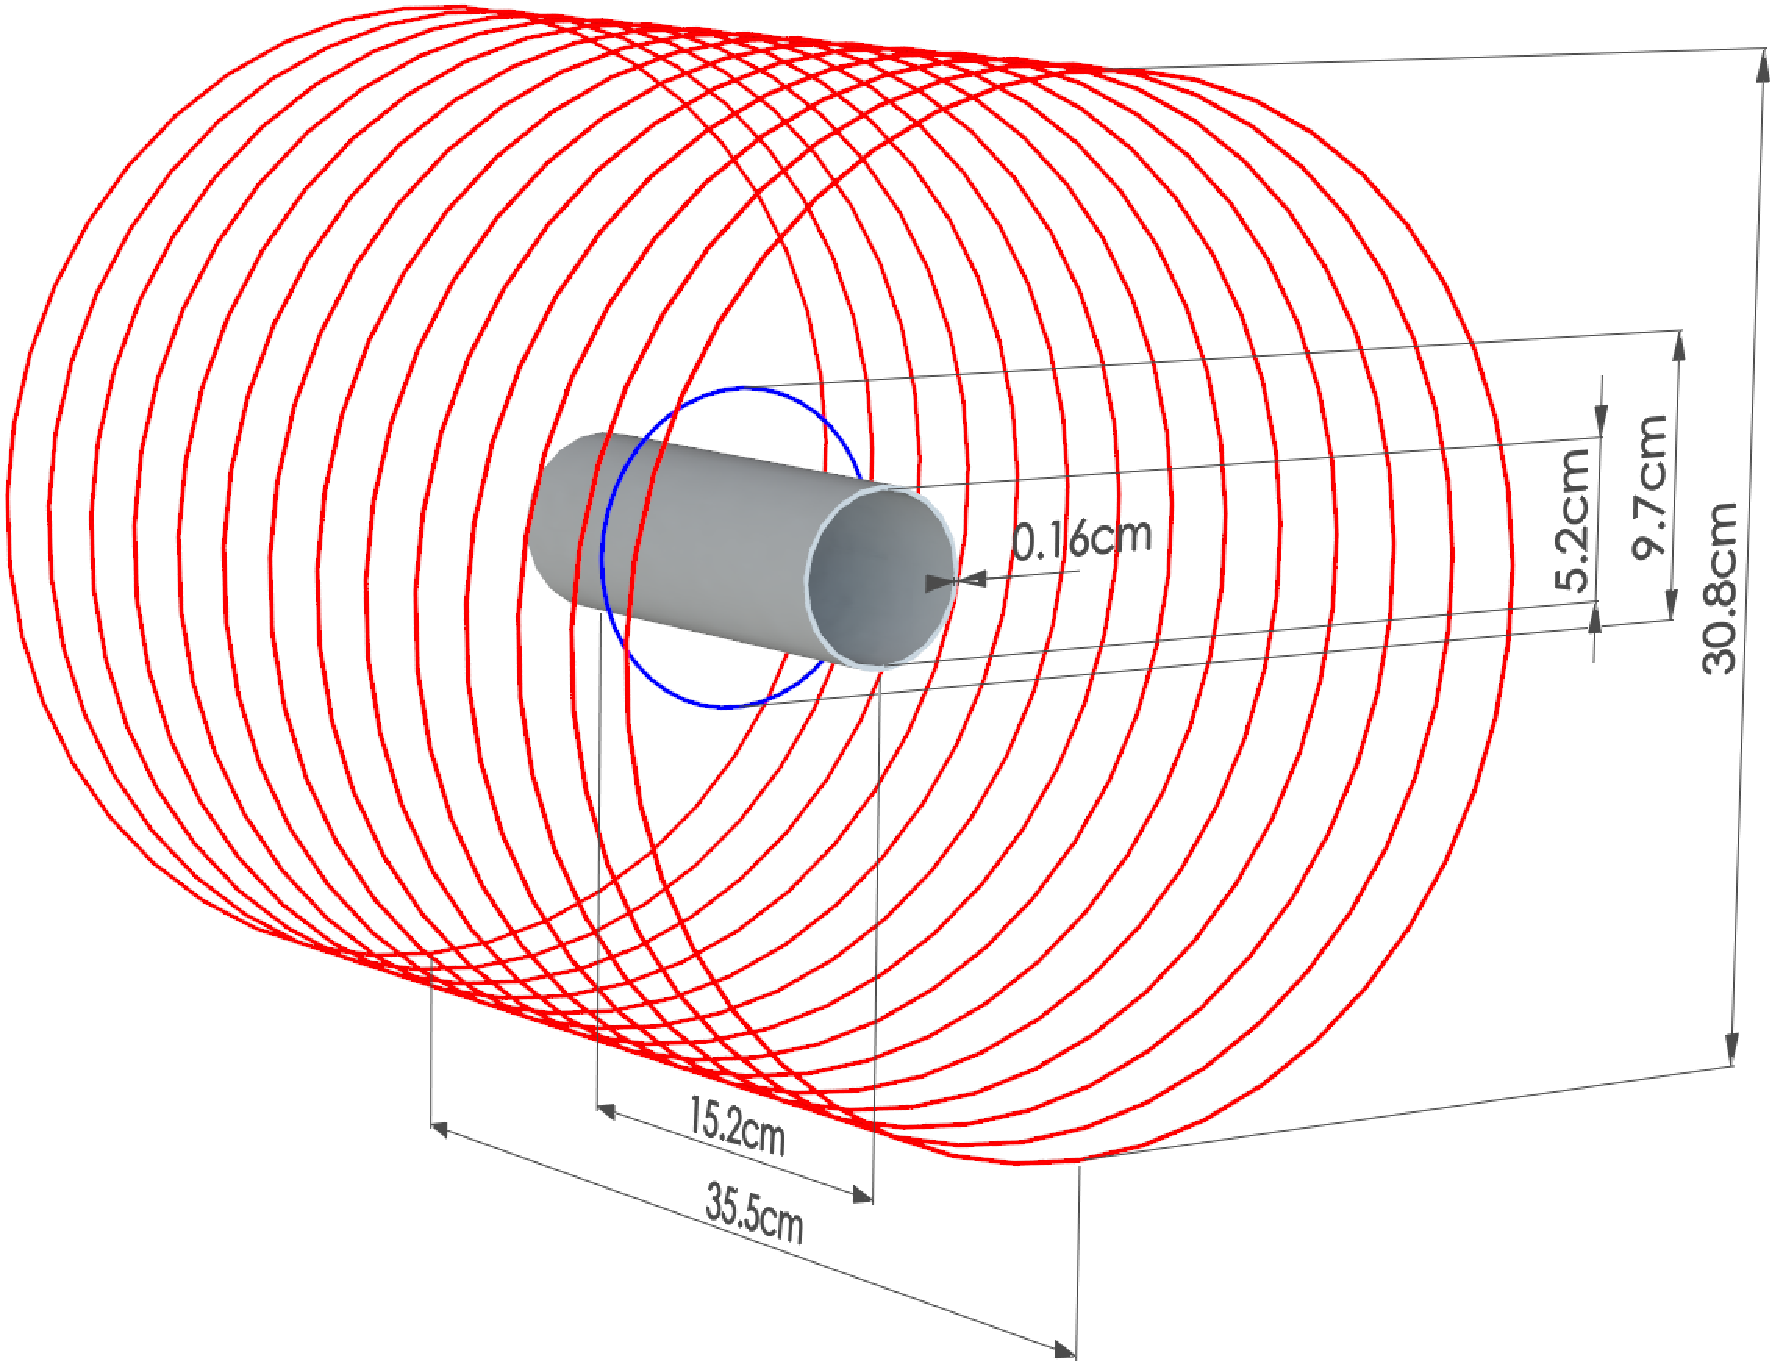
\includegraphics[width=0.7\textwidth]{to_jeff_new4.pdf}
    \caption[Drawing of the axial shielding factor measurement setup
    ]{Axial shielding factor measurement setup. The witness cylinder
      with an inner diameter of 5.2~cm and a length of 15.2~cm is
      placed inside a solenoid (shown in red) with a diameter of
      30.8~cm and a length of 35.5~cm, containing 14 turns.  The
      thickness of the witness cylinder is $1/16''=0.16$~cm.  The loop
      coil (shown in blue) is mechanically coupled to the witness
      cylinder and has a diameter of 9.7~cm.}
    \label{fig:geometry}
  \end{center}
\end{figure}

As shall be described in Section~\ref{sec:axialsyst}, a concern in the
measurement was changes in the field measured by the fluxgate that
could arise due to motion of the system components, or other
temperature dependences. This could generate a false slope with
temperature that might incorrectly be interpreted as a change in the
magnetic properties of the witness cylinder.

To address possible motion of the witness cylinder with respect to the
field generation system, another coil (the loop coil, also shown in
Fig.~\ref{fig:geometry}) was wound on a plastic holder mounted rigidly
to the witness cylinder.  The coil was one loop of copper wire with a
diameter of 9.7~cm.  Plastic set screws in the holder fixed the loop
coil to be coaxial with the witness cylinder.

Systematic differences in the results from the two coils (the
solenoidal coil, and the loop coil) were used to search for motion
artifacts.  As well, some differences could arise due to the different
magnetic field produced by each coil, and so such measurements could
reveal a dependence on the profile of the applied magnetic field.
This is described further in Section~\ref{sec:axialsyst}.

The temperature of the witness cylinder was measured by attaching four
thermocouples at different points along the outside of the cylinder.
This allowed us to observe the temperature gradient along the witness
cylinder.  To reduce any potential magnetic contamination, T-type
thermocouples were used, which have copper and constantan conductors.
(K-type thermocouples are magnetic.)

Thermocouple readings were recorded by a National Instruments NI-9211
temperature input module.  The magnetic field (signified by the
lock-in amplifier readout) and the temperature were recorded at a rate
of 0.2~Hz.

Temperature variations in the experiment were driven by ambient
temperature changes in the room, although forced air and other
techniques were also tested.  These are described further in
Section~\ref{sec:axialsyst}.


\subsubsection{Data and Interpretation\label{sec:axialsyst}}

An example of the typical data acquired is shown in
Fig.~\ref{fig:B_vs_Temp}.  For these data, the field applied by the
solenoid coil was 1~$\mu$T in amplitude, at a frequency of 1~Hz.
Fig.~\ref{fig:B_vs_Temp}(a) shows the temperature of the witness
cylinder over a 70-hr measurement.  The temperature changes of 1.4~K
are caused by diurnal variations in the laboratory.  The shielded
magnetic field amplitude $B_s$ within the witness cylinder is
anti-correlated with the temperature trend as shown in
Fig.~\ref{fig:B_vs_Temp}(b).  Here, $B_s$ is the sum in quadrature of
the amplitudes of the in-phase and out-of-phase components (most of
the signal is in phase).  The magnetic field is interpreted to depend
on temperature, and the two quantities are graphed as a function of
one another in Fig.~\ref{fig:B_vs_Temp}(c).  The slope in
Fig.~\ref{fig:B_vs_Temp}(c) has been calculated using a linear fit to
the data.  The relative slope at 23$^\circ$C was found to be
$\frac{1}{B_s}\frac{dB_s}{dT}=-0.75\%$/K.

\begin{figure}
  \begin{center}
    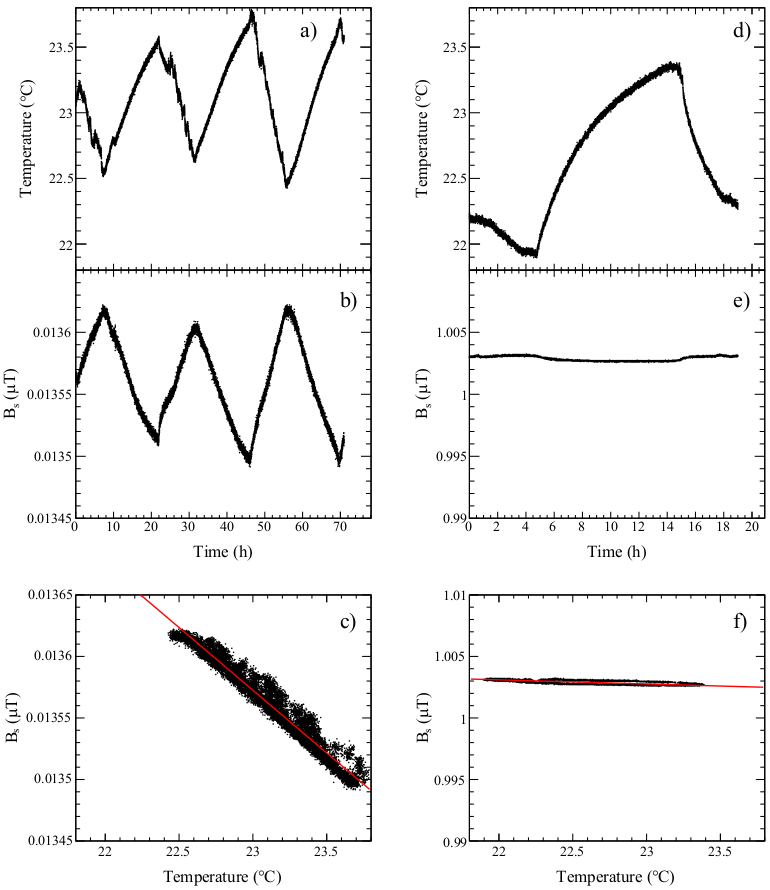
\includegraphics[width=\textwidth]{fig3.png}
    \caption[Ambient temperature and shielded magnetic field amplitude
    measurement]{Ambient temperature and shielded magnetic field
      amplitude, measured over a 70 hour period. (a) temperature of
      the witness cylinder as a function of time.  (b) magnetic field
      amplitude measured by fluxgate at center of witness cylinder
      vs.~time.  (c) magnetic field vs.~temperature with linear fit to
      data giving $\frac{1}{B_s}\frac{dB_s}{dT}=-0.75\%$/K (evaluated
      at 23$^\circ$C).  In panels (d), (e), and (f), the same
      quantities are shown for a 20-hour run with a copper cylinder in
      place of the witness cylinder with the linear fit giving
      $\frac{1}{B_s}\frac{dB_s}{dT}=-0.03\%$/K.}
    \label{fig:B_vs_Temp}
  \end{center}
\end{figure} 

Figs.~\ref{fig:B_vs_Temp}(d), (e), and (f) show the same measurement
with essentially the same settings, when the mu-metal witness cylinder
is replaced by a copper cylinder.  A similar relative vertical scale
has been used in Figs.~\ref{fig:B_vs_Temp}(e) and (f) as
Figs.~\ref{fig:B_vs_Temp}(b) and (c).  This helps to emphasize the
considerably smaller relative slope derived from panel (f) compared to
panel (c).  A variety of measurements of this sort were carried out
multiple times for different parameters such as coil current.  Running
the coil at the same current tests for effects due to heating of the
coil, whereas running the coil at a current which equalizes the
fluxgate signal to its value when the mu-metal witness cylinder is
present tests for possible effects related to the fluxgate.  For all
measurements the temperature dependence of the demodulated magnetic
signal was $<0.1$\%/K, giving confidence that unknown systematic
effects contribute below this level.

Some deviations from the linear variation of $B_s$ with $T$ can be
seen in the data, particularly in Figs.~\ref{fig:B_vs_Temp}(a), (b),
and (c).  For example, when the temperature changes rapidly, the
magnetic field takes some time to respond, resulting in a slope in
$B_s-T$ space that is temporarily different than when the temperature
is slowly varying.  This is typical of the data that we acquired, that
the data would generally follow a straight line if the temperature
followed a slow and smooth dependence with time, but the data would
not be linear if the temperature varied rapidly or non-monotonically
with time.  We also tried other methods of temperature control, such
as forced air, liquid flowing through tubing, and thermo-electric
coolers.  The diurnal cycle driven by the building's air conditioning
system gave the most stable method of control and the most
reproducible results for temperature slopes.

As mentioned earlier, data were acquired for both the solenoid coil
and the loop coil. A summary of the data is provided in
Table~\ref{tab:axial}.  Repeated measurements of temperature slopes
using the loop coil fell in the range
0.4\%/K~$<\vert\frac{1}{B_s}\frac{dB_s}{dT}\vert<$~1.5\%/K.  Similar
measurements for the solenoidal coil yielded
0.3\%/K~$<\vert\frac{1}{B_s}\frac{dB_s}{dT}\vert<$~0.8\%/K.

\begin{table}
\begin{center}
\begin{tabular}{cccc}\hline
Trial & $\frac{1}{B_s}\frac{dB_s}{dT}$ & Coil \\
\#    & (\%/K) & type \\\hline
 1 & -0.32 & solenoid \\
 2 & -0.30 & solenoid \\
 3 & -0.33 & solenoid \\
 4 & -1.53 & loop \\
 5 & -0.42 & loop \\
 6 & -1.30 & loop \\
 7 & -0.74 & solenoid \\
 8 & -1.05 & loop \\
 9 & -0.73 & solenoid \\
10 & -1.23 & loop \\
11 & -0.75 & solenoid \\
12 & -1.12 & loop \\\hline
\end{tabular}
\caption[Summary of the AC axial shielding factor
measurements]{Summary of data acquired for the AC axial shielding
  factor measurements, in chronological order.  Data with an applied
  field of $\sim 1-6~\mu T$ and a measurement frequency of 1~Hz are
  included.  Data which used daily fluctuations of the temperature
  from 21-24$^\circ$C over a 10-80 hour period are included.  Other
  data acquired for systematic studies are not included in the
  table.\label{tab:axial}}
\end{center}
\end{table}

In general, the slopes measured with the loop coil were larger than
for the solenoidal coil.  This is particularly evident for
measurements 6-12, which were acquired daily over the course of a few
weeks alternating between excitation coils but all used the same
witness cylinder and otherwise without disturbing the measurement
apparatus.  A partial explanation of this difference is offered by the
field profile generated by each coil, and its interaction with the
witness cylinder.  This is addressed further in
Section~\ref{sec:axialsims}.

The other difference between the loop coil and the solenoidal coil was
that the loop coil was rigidly mounted to the witness cylinder,
reducing the possibility of artifacts from relative motion.  Given
that this did not reduce the range of the measured temperature slopes
we conclude that relative motion was well controlled in both cases.

Several other possible systematic effects were considered, all of
which were found to give uncertainties on the measured slopes
$<0.1\%$/K.  These included: thermal expansion of components including
the witness cylinder itself, temperature variations of the magnetic
shielding system within which the experiments were conducted,
degaussing of the witness cylinder, and temperature slopes of various
components e.g. the fluxgate magnetometer and the lock-in amplifier.

%%% null meast
As mentioned earlier in reference to Fig.~\ref{fig:B_vs_Temp}(d), (e),
and (f), the stability of the system was also tested by replacing the
mu-metal witness cylinder with a copper cylinder and in all cases
temperature slopes $<0.1$\%/K were measured, giving confidence that
other unknown systematic effects contribute below this level.

Based on the systematic effects that we studied, we conclude that they
do not explain the ranges of values measured for
$\frac{1}{B_s}\frac{dB_s}{dT}$.  We suspect that the range measured is
either some yet uncharacterized systematic effect, or a complicated
property of the material. We use this range to set a limit on the
slope of $\mu(T)$


\subsubsection{Geometry correction and determination of $\mu(T)$\label{sec:axialsims}}

To relate the data on $B_s(T)$ to $\mu(T)$, the shielding factor of
the witness cylinder as a function of $\mu$ must be known. Finite
element simulations in FEMM and OPERA were performed to determine this
factor.  The simulations are also useful for determining the effective
values of $B_m$ and $H_m$ in the material, which will be useful to
compare to the case for typical nEDM experiments when the innermost
shield is used as a flux return.

For closed objects, such as spherical
shells~\cite{bidinosti2014passive, urankar1996design}, the shielding
factor approaches infinity as $\mu \rightarrow \infty$, and
$\vert\frac{\mu}{B_s}\frac{dB_s}{d\mu}\vert\rightarrow 1$.  Because
the witness cylinders are open ended, the shielding factor
asymptotically approaches a constant rather than infinity in the
high-$\mu$ limit, and as a result
$\vert\frac{\mu}{B_s}\frac{dB_s}{d\mu}\vert<1$ here.  From the
simulations the ratio $\frac{\mu}{B_s}\frac{dB_s}{d\mu}$ was
calculated.  A linear model of the material was used where
$\bold{B_m}=\mu\bold{H_m}$ with $\mu$ constant.


The simulations differed slightly in their results, dependent on
whether OPERA or FEMM was used, and whether the solenoidal coil or
loop coil were used.  Based on the simulations, the result is
$\vert\frac{\mu}{B_s}\frac{dB_s}{d\mu}\vert=0.42-0.50$ for the
solenoidal coil, with the lower value being given by FEMM and the
upper value being given by a 3D OPERA simulation, for identical
geometries.  This is somewhat lower than the value suggested by
Ref.~\cite{paperno1999charts} with fits to simulations performed
in OPERA, which we estimate to be 0.6.  We adopt our value since it is
difficult to determine precisely from
Ref.~\cite{paperno1999charts}.  For the loop coil, we determine
$\vert\frac{\mu}{B_s}\frac{dB_s}{d\mu}\vert=0.56-0.65$, the range
being given again by a difference between FEMM and OPERA.

Combining the measurement and the simulations, the temperature
dependence of the effective $\mu$ (at $\mu_r=20,000$ which is
consistent with our measurements) can be calculated by
equation~(\ref{eqn:axial}).  The results of the simulations and
measurements are presented in Table~\ref{tab:axialsummary}. Combining
the loop coil and solenoidal coil results, we find
0.6\%/K~$<\frac{1}{\mu}\frac{d\mu}{dT}<2.7\%$/K to represent the full
range for the possible temperature slope of $\mu$ that observed in
these measurements.

\begin{table}
\begin{center}
\begin{tabular}{|c|c|c|c|}
\hline 
  & $\vert \frac{\mu}{B_s}\frac{dB_s}{d\mu}\vert$ & $\vert \frac{1}{B_s} \frac{dB_s}{dT}\vert$~(\%/K) & $\frac{1}{\mu}\frac{d\mu}{dT}$~(\%/K) \\ 
 & (simulated) & (measured) & (extracted) \\
\hline 
Solenoidal Coil & 0.42-0.50 & 0.3-0.8 & 0.6-1.9 \\ 
\hline 
Loop Coil & 0.56-0.65 & 0.4-1.5 & 0.6-2.7 \\ 
\hline 
\end{tabular} 
\caption[Summary of finite element simulations and shielding factor
measurements]{Summary of OPERA and FEMM simulations and shielding
  factor measurements, resulting in extracted temperature slopes of
  $\mu$.}
\label{tab:axialsummary}
\end{center}

\end{table}


As stated earlier, the simulations also provided a way to determine
the typical $B_m$ and $H_m$ internal to the material of the witness
cylinder.  According to the simulations, the $B_m$ amplitude was
typically 100~$\mu$T and the $H_m$ amplitude was typically 0.004~A/m.
These are comparable to the values normally encountered in nEDM
experiments, recalling from Section~\ref{sec:calculation} that
$H_m<0.007$~A/m for the innermost magnetic shield of an nEDM
experiment.  A caveat is that these measurements were typically
conducted using AC fields at 1~Hz, as opposed to the DC fields
normally used in nEDM experiments.


% Transformer core measurements Section moved to transformer.tex


\subsection{Transformer Core Measurements}
\label{sec:transformer}

An alternative technique similar to the standard method of magnetic
materials characterization via magnetic induction was also used to
measure changes in $\mu$.  In this measurement technique, the witness
cylinder was used as the core of a transformer.  Two coils (primary
and secondary) were wound on the witness cylinder using multistranded
20-gauge copper wire.  The windings were made as tight as possible,
but not so tight as to potentially stress the material.  The windings
were not potted in place.  Three witness cylinders were tested.  Data
were acquired using different numbers of turns on both the primary and
secondary coils (from 6 to 48 on the primary, and from 7 to 24 on the
secondary).

Fig.~\ref{fig:transformer} shows a picture of one of the witness
cylinders, wound as described.  It also shows a schematic diagram of
the measurement setup, which we now use to describe the measurement
principle.

\begin{figure}[h!]
  \begin{center}
    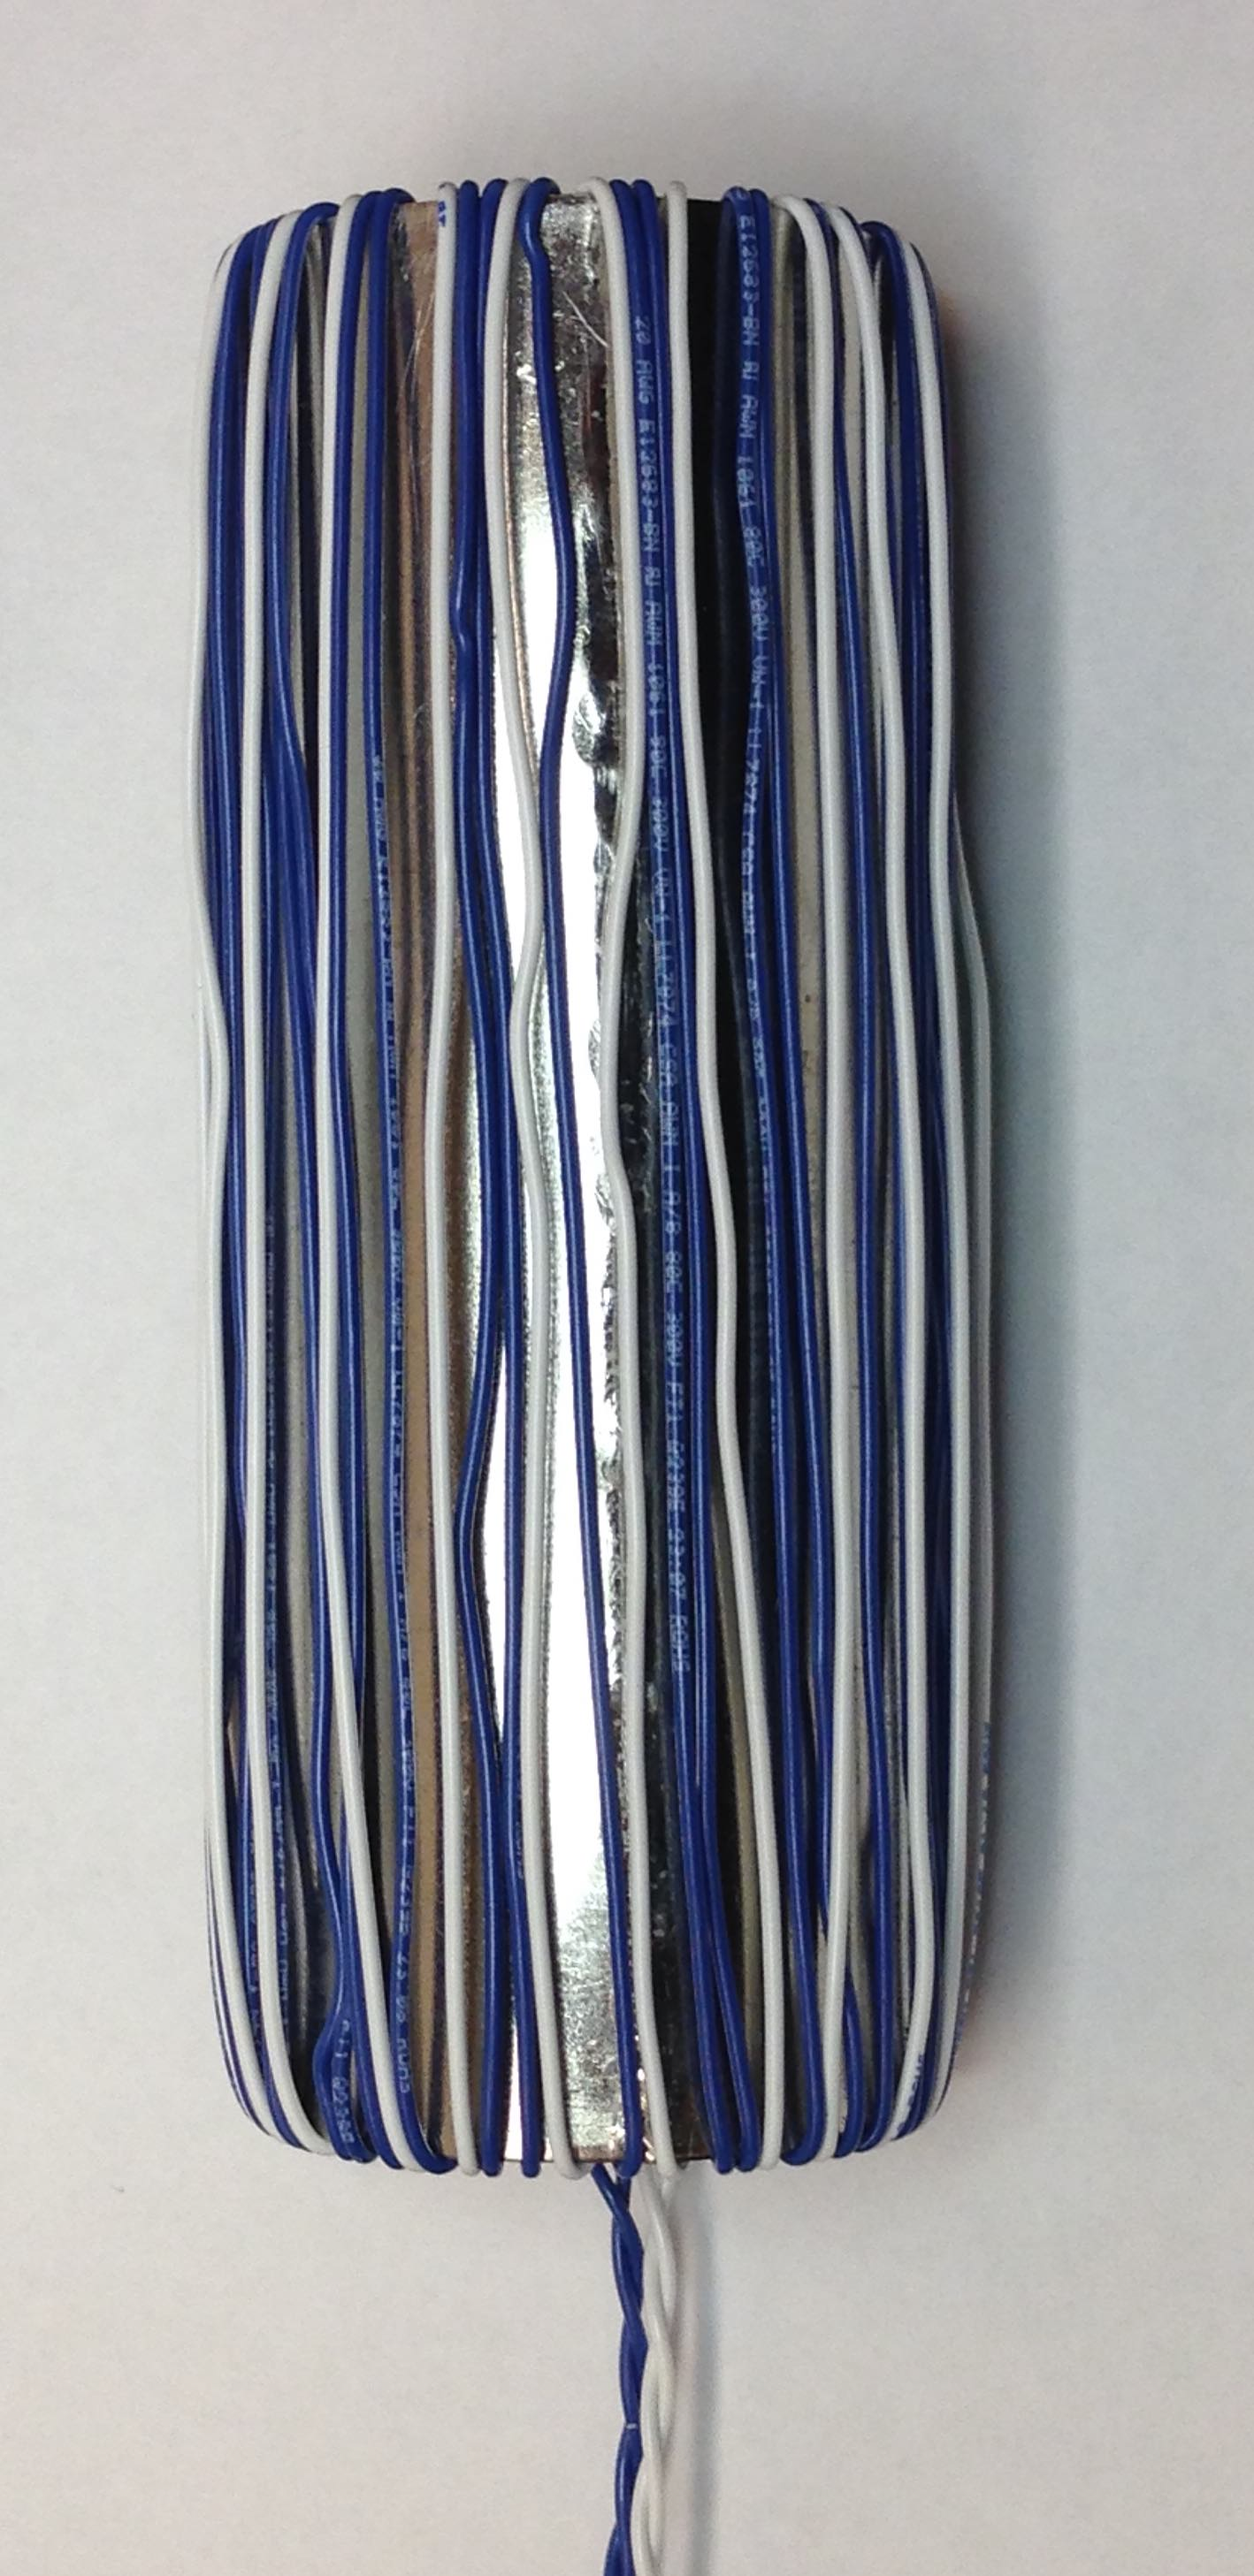
\includegraphics[height=3cm]{picture.png}\hskip1cm
    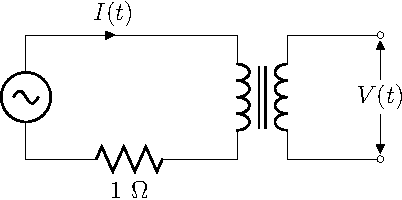
\includegraphics[height=3cm]{figure4-crop.pdf}
    \caption[ Photograh and schematic of the transformer
    measurements]{Photograph of a witness cylinder showing transformer
      windings (left) and schematic of the transformer measurement
      (right).  The primary coil was driven by the sine-out of an
      SR830 lock-in amplifier, which was also used to demodulate
      induced voltage $V(t)$ in the secondary coil. The driving
      current $I(t)$ was sensed by measuring the voltage across a
      stable 1~$\Omega$ resistor.}
    \label{fig:transformer}
  \end{center}
\end{figure}


% Table 9 on page 65 of Taraneh's report shows the different windings.
% Can guess which core is which.

%In the end, a transformer with 48 windings on the primary and 21
%windings on the secondary was used.

%This enabled more saturation of the material.

The primary coil generated an AC magnetic field as a function of time
$H(t)$, while the secondary coil was used to measure the emf induced
by the time-varying magnetic flux proportional to $dB(t)/dt$.  To a
good approximation
\begin{equation}
H_m(t)=\frac{N_pI(t)}{2\pi R}
\end{equation}
where $N_p$ is the number of turns in the primary, $I(t)$ is the
current in the primary, and $R$ is the radius of the witness cylinder,
and
\begin{equation}
\frac{dB_m(t)}{dt}=\dot{B}_m(t)=\frac{V(t)}{b\ell}
\label{eqn:bdot}
\end{equation}
where $V(t)$ is the voltage generated in the secondary, and $b$ and
$\ell$ are the thickness and length of the witness cylinder
respectively.  For a sinusoidal drive current $I(t)$, and under the
assumption that $B_m(t)=\mu H_m(t)$ with $\mu$ being a constant, the
voltage generated in the secondary $V(t)$ should be sinusoidal and out
of phase with the primary current.

The internal oscillator of an SR830 lock-in amplifier was used to
generate $I(t)$.  This was monitored by measuring the voltage across a
1~$\Omega$ resistor with small temperature coefficient in the primary
loop. The lock-in amplifier was then used to demodulate $V(t)$ into
its in-phase $V_X$ and out-of-phase $V_Y$ components (or equivalently
$\dot{B}_m(t)$ being demodulated into $\dot{B}_{m,X}$ and
$\dot{B}_{m,Y}$, as in equation~(\ref{eqn:bdot})).  The experiment was
done at 1~Hz with $H_m(t)$ as small as possible, typically 0.1~A/m in
amplitude, to measure the slope of the minor $B_m-H_m$ loops near the
origin of the $B_m-H_m$ space.

The temperature of the core was measured continuously using the same
thermocouple arrangement described previously. Measurements of $V_Y$
as a function of temperature would then signify a change in $\mu$ with
temperature.  In general, we used ambient temperature variations for
the measurements, similar to the procedure used for our axial
shielding factor measurements.

% Although we would have preferred to measure at even lower frequencies
% and amplitudes, these settings were found to be the minimum possible
% before noise would make it impossible to measurement the long-term
% (hours) evolution of the $X$ and $Y$ readings.

The naive expectation is that the out-of-phase $V_Y$ component should
signify a non-zero $\mu$, and the in-phase $V_X$ component should be
zero.  In practice, due to a combination of saturation, hysteresis,
eddy-current losses, and skin-depth effects, the $V_X$ component is
nonzero.  It was found experimentally that keeping the amplitude of
$H_m(t)$ small compared to the apparent coercivity ($\sim 3$~A/m for
the 0.16~cm thick material at 1~Hz frequencies) ensured that the $V_Y$
component was larger than the $V_X$ component.  This is displayed
graphically in Fig.~\ref{fig:data_and_simulation}, where the
dependence of $\dot{B}_{m,Y}$ and $\dot{B}_{m,X}$ on the amplitude of
the applied $H_m(t)$ is displayed, for a driving frequency of 1~Hz.
Clearly the value of $\dot{B}_{m,X}$ can be considerable compared to
$\dot{B}_{m,Y}$, for larger $H_m$ amplitudes near the coercivity.  At
larger amplitudes, the material goes into saturation.  Both
$\dot{B}_{m,Y}$ and $\dot{B}_{m,X}$ eventually decrease as expected at
amplitudes much greater than the coercivity.

To understand the behavior in Fig.~\ref{fig:data_and_simulation}, a
theoretical model of the hysteresis based on the work of
Jiles~\cite{jiles1994frequency} was used.
%The model contains a number
%of adjustable parameters.
The anhysteretic magnetization of a material in the presence of
magnetic field could be written as
\begin{equation}
M_{an}(H) =  M_s \ell \left( \frac{H + \alpha M_{an}(H)}{a} \right)
\end{equation}
where $\ell$ is the langevin function $\ell = coth(x) - 1/x$, $M_s$ is
the saturation magnetization, $\alpha$ is a coupling coefficient,
$a = k_BT/\mu_0 <m> $ with $k_B$ being the Bolzmann constant, $T$
being the temperature, $\mu_0$ the permeability of free space, and
$<m>$ is the effective domain size. The equation for hysteresis can then be derived from the energy-balance equation 
\begin{equation}
\mu_0 \int M_{an} dH_e  = \mu_0 \int M dH_e + \mu_0 k \delta(1-c) \int \frac{dM_{irr}}{dH_e}~,
\end{equation}
which means, in an initially demagnetized material, hysteresis can
appear as a change in total demagnetization, or or be dissipated due
to irreversible changes in magnetization $M_{irr}$ (hysteresis
loss). Here the first term of the right-hand side is the contribution
to the magnetostatic energy, and the second term on the right-hand
side is the dissipation loss due to pinning. In this equation
$H_e= H + \alpha M$, the coefficient $k$ is the pinning parameter
which determines the amount of energy dissipated, and $\delta$ is a
directional parameter which ensures that energy is always lost through
dissipation. The coefficient $c$ is a measure of the amount of
reversible change in magnetization.  The total magnetization cosists
of two parts including reversible and irreversible magnetization
$M = M_{\mathrm{irr}} + M_{\mathrm{rev}}$.

Now including both classical (eddy current) losses and anomalous
losses we get
\begin{equation}
  \begin{aligned}
    &\left (  \frac{\mu_0d^2}{2 \rho \beta} \frac{dH}{dt} \right)\left( \frac{dM}{dH} \right)+ \left (\frac{GdW\mu_0 H_0}{\rho} \right)^2 \left( \frac{dH}{dt} \right)^2 \left( \frac{dM}{dH} \right)^{3/2} \\
    &+ \left[k\delta - \alpha \left( M_{an}(H) - M(H) + k \delta c \frac{dM_{an}}{dH_e}\right)\right] \left( \frac{dM}{dH} \right) \\
    &- \left(M_{an}(H) - M(H) + k \delta c\frac{dM_{an}}{dH_e} \right) = 0~,
  \end{aligned}
\end{equation}
where $\rho$ is the resistivity, $d$ is the cross-sectional dimension
in meters, $\beta$ is a geometric factor, $G$ is a dimensionless
constant of value 0.1356, $w$ is the width of the laminations, $H_0$
is a parameter representing the fluctuating internal potential
experienced by domain walls. This equation can be solved numerically.


We adjusted the parameters based on our
measurements of $B_m-H_m$ loops including the initial magnetization
curve.  These measurements were performed separately from our lock-in
amplifier measurements, using an arbitrary function generator and a
digital oscilloscope to acquire them.  The measurements were done at
frequencies from 0.01 to 10~Hz.  It was found that the frequency
dependence predicted by Ref.~\cite{jiles1994frequency} gave relatively good
agreement with the measured $B_m-H_m$ loops once the five original
(Jiles-Atherton~\cite{jiles1984theory,jiles1986theory}) parameters were tuned.

For the parameters of the (static) Jiles-Atherton model, we used
$B_s=0.45$~T, $a=3.75$~A/m, $k=2.4$~A/m, $\alpha=2\times 10^{-6}$,
$c=0.05$, which were tuned to our $B_m-H_m$ curve measurements.  For
classical losses, we used the parameters $\rho=5.7\times
10^{-7}~\Omega\cdot$m, $d=1.6$~mm (the thickness of the material), and
$\beta=6$ (geometry factor).  These parameters were not tuned, but
taken from data.  For anomalous losses we used the parameters
$w=0.005$~m and $H_0=0.0075$~A/m, which we also did not tune, instead
relying on the tuning performed in Ref.~\cite{jiles1994frequency}.

These parameters were then used to model the measurement presented in
Fig.~\ref{fig:data_and_simulation}, including the lock-in amplifier
function.  As shown in Fig.~\ref{fig:data_and_simulation}, trends in
the measurements and simulations are fairly consistent.  The sign of
$\dot{B}_{m,X}$ relative to $\dot{B}_{m,Y}$ is also correctly
predicted by the model (we have adjusted them both to be positive, for
graphing purposes).  We expect that with further tuning of the model,
even better agreement could be achieved.

\begin{figure}[h!]
  \begin{center}
    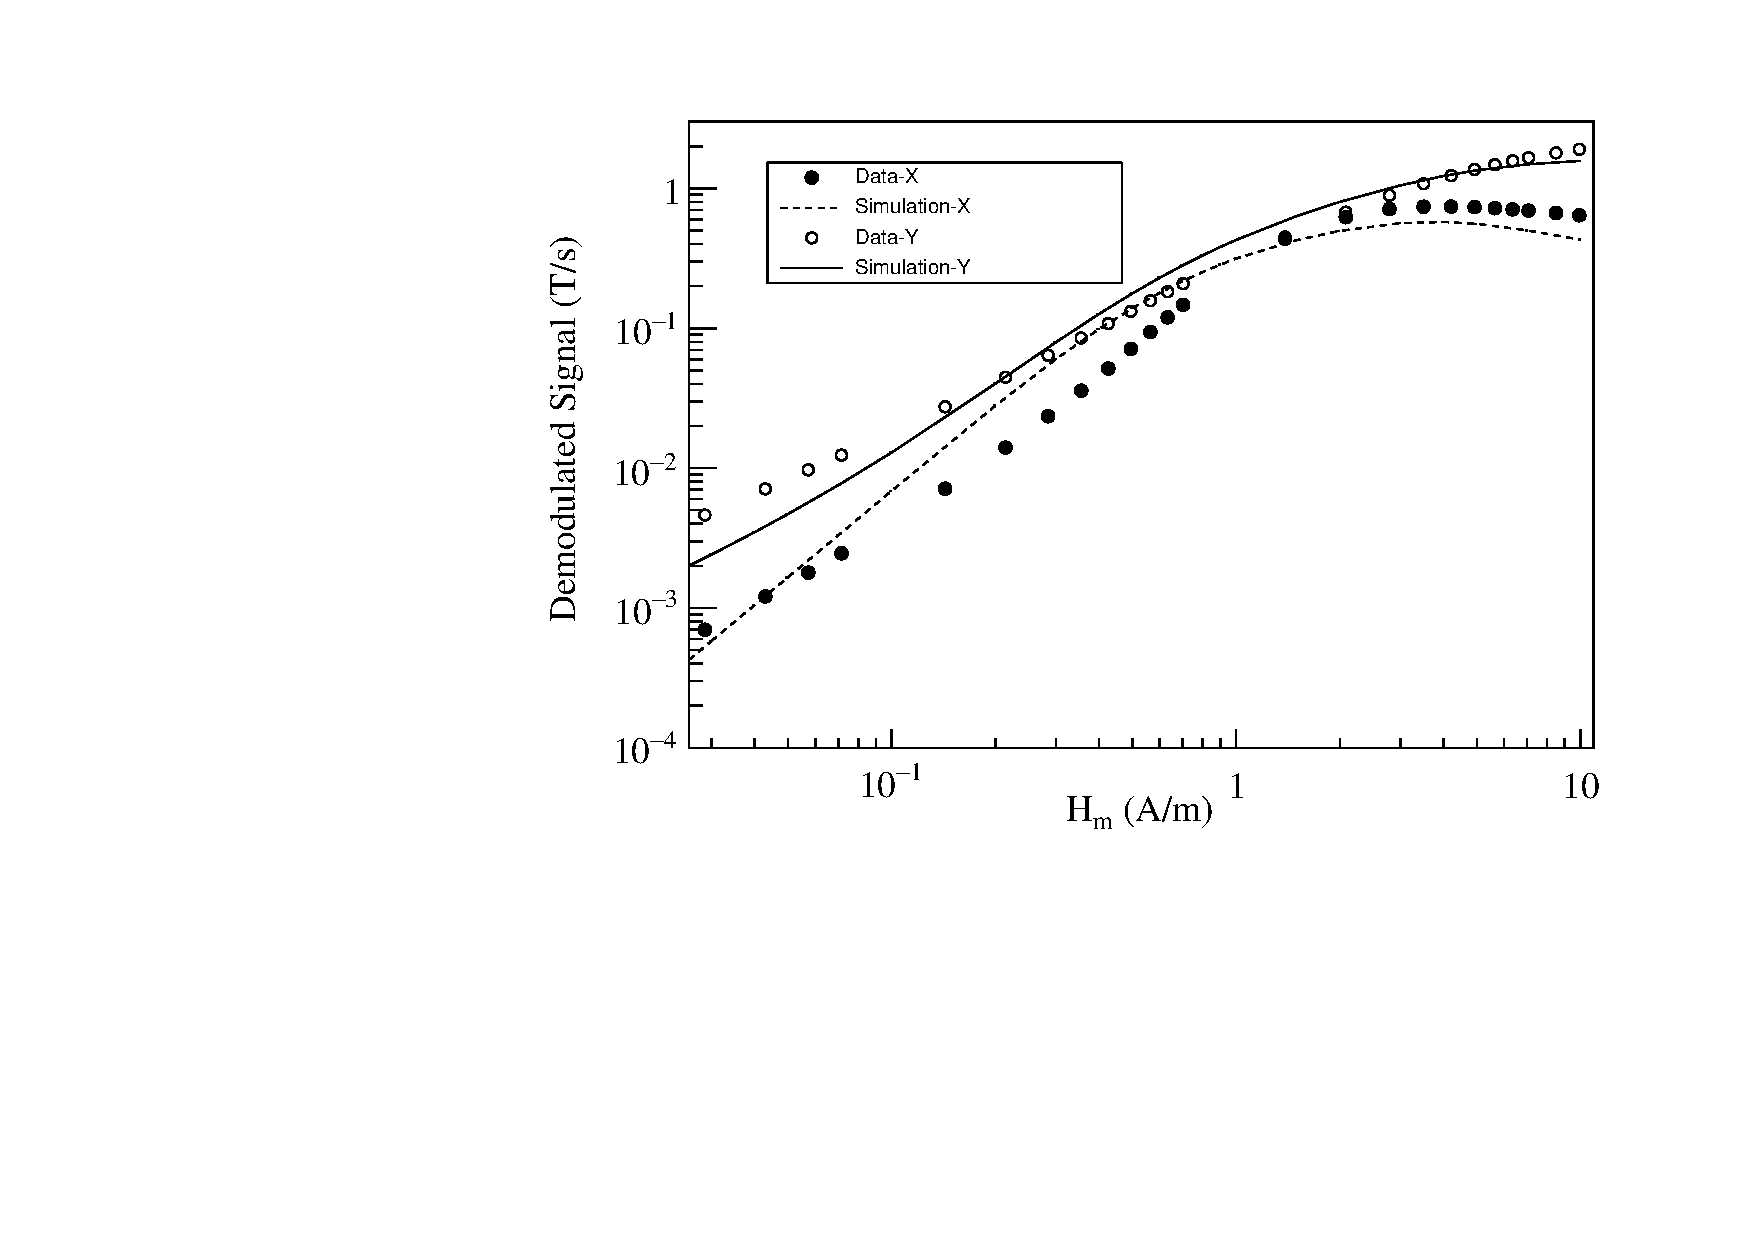
\includegraphics[width=\textwidth]{Jiles_and_data.pdf}
    \caption[Demodulated signal as a function of amplitude of the
    applied $H_m$ field]{$\dot{B}_{m,X}$ and $\dot{B}_{m,Y}$ as a
      function of amplitude of the applied $H_m$ field at 1~Hz.
      Points show the acquired data.  Curves display the simulation
      based on the model described in the text.}
    \label{fig:data_and_simulation}
  \end{center}
\end{figure} 

The model of Ref.~\cite{jiles1994frequency} makes no prediction of the
temperature dependence of the parameters.  Ideally, the temperature
dependence of $\dot{B}_{m,Y}$ and $\dot{B}_{m,X}$ under various
conditions could be used to map out the temperature dependence of the
parameters.  However, this is beyond the scope of the present work.

We make the simplifying assumption that temperature dependence of
$\dot{B}_{m,Y}$ may be approximately interpreted as the temperature
dependence of a single parameter $\mu$, i.e. that
\begin{equation}
\frac{1}{\dot{B}_{m,Y}}\frac{d\dot{B}_{m,Y}}{dT}=\frac{1}{\mu}\frac{d\mu}{dT}.
\end{equation}
This is justified in part by our selection of measurement parameters
(the amplitude of $H_m=0.1$~A/m and a measurement frequency of 1~Hz)
which ensure that $\dot{B}_{m,Y}$ dominates over $\dot{B}_{m,X}$.

We assign no additional systematic error for this simplification, and
all our results are subject to this caveat.  We comment further that
in our measurements of the axial shielding factor (presented in
Section~\ref{sec:axial}), the same caveat exists.  In that case the
in-phase component dominates the demodulated fluxgate signal.  In a
sense, measuring $\mu(T)$ itself is always an approximation, because
it is actually the parameters of minor loops in a hysteresis curve
which are measured.  In reality, our results may be interpreted as a
measure of the temperature-dependence of the slopes of minor loops
driven by the stated $H_m$.

Measurements of $\frac{1}{\dot{B}_{m,Y}}\frac{d\dot{B}_{m,Y}}{dT}$ as
a function of $T$ were made.  In general, the data mimicked the
behavior of the axial shielding factor measurements, giving a similar
level of linearity with temperature as the data displayed in
Fig.~\ref{fig:B_vs_Temp}.  Other similar behaviors to those
measurements were also observed, for example: (a) when the temperature
slope changed sign, $\dot{B}_{m,Y}$ would temporarily give a different
slope with temperature, (b) the measured value of
$\frac{1}{\dot{B}_{m,Y}}\frac{d\dot{B}_{m,Y}}{dT}$ depended on a
variety of factors, most notably a dependence on which of the three
witness cylinders was used for the measurement, and on differences
between subsequent measurements using the same cylinder.

\begin{table}
\begin{center}
\begin{tabular}{cccc}\hline
Trial & $\frac{1}{\dot{B}_{m,Y}}\frac{d\dot{B}_{m,Y}}{dT}$ & core \\
\#    & (\%/K) & used \\\hline
 1 & 0.15 & $\alpha$ \\
 2 & 0.03 & $\alpha$ \\
 3 & 0.04 & $\alpha$ \\
 4 & 0.06 & $\alpha$ \\
 5 & 1.07 & $\beta$  \\
 6 & 0.93 & $\beta$  \\
 7 & 0.88 & $\beta$  \\
 8 & 0.88 & $\beta$  \\
 9 & 0.09 & $\alpha$ \\
10 & 1.23 & $\beta$  \\
11 & 2.15 & $\beta$  \\
12 & 1.85 & $\beta$  \\
13 & 1.20 & $\beta$  \\
14 & 0.77 & $\gamma$ \\\hline
\end{tabular}
\caption[Summary of transformer core meaurement data]{Summary of data
  acquired for the transformer core measurements.  Three different
  witness cylinders, arbitrarily labeled $\alpha$, $\beta$, and
  $\gamma$, were used for the measurements.  A 1~Hz excitation
  frequency was used with amplitudes for $H_m$ ranging from 0.1 to
  0.3~A/m.  Fluctuations in the temperature ranged from 21-24$^\circ$C
  and measurement times over a 10-80 hour period are included.  Other
  data acquired for systematic studies are not included in the
  table.\label{tab:transformer}}
\end{center}
\end{table}



Table~\ref{tab:transformer} summarizes our measurements of the
relative slope $\frac{1}{\dot{B}_{m,Y}}\frac{d\dot{B}_{m,Y}}{dT}$ for
a variety of trials, witness cylinders, and numbers of windings.  The
data show a full range of $0.03-2.15$\%/K for
$\frac{1}{\mu}\frac{d\mu}{dT}=\frac{1}{\dot{B}_{m,Y}}\frac{d\dot{B}_{m,Y}}{dT}$,
again naively assuming the material to be linear as discussed above.
The sign of the slope of $\mu(T)$ was the same as the axial shielding
factor technique.

A dominant source of variation between results in this method arose
from properties inherent to each witness cylinder.  One of the
cylinders (referred to as $\beta$ in Table~\ref{tab:transformer}) gave
temperature slopes consistently larger
$\frac{1}{\mu}\frac{d\mu}{dT}\sim 0.88-2.15$\%/K than the other two
$\frac{1}{\mu}\frac{d\mu}{dT}\sim 0.03-0.77$\%/K (referred to as
$\alpha$ and $\gamma$, with some evidence that $\gamma$ had a larger
slope than $\alpha$).  We expect this indicates some difference in the
annealing process or subsequent treatment of the cylinders, although
to our knowledge the treatment was controlled the same as for all
three cylinders.  Since our goal is to provide input to future EDM
experiments on the likely scale of the temperature dependence of $\mu$
that they can expect, we phrase our result as a range covering all
these results.

Detailed measurements of the effect of degaussing were conducted for
this geometry.  The ability to degauss led us ultimately to select a
larger number of primary turns (48) so that we could fully saturate
the core using only the lock-in amplifier reference output as a
current source.  A computer program was used to control the lock-in
amplifier in order to implement degaussing.  A sine wave with the
measurement frequency (typically 1~Hz) was applied at the maximum
lock-in output power.  Over the course of several thousand
oscillations, the amplitude was decreased linearly to the measurement
amplitude ($\sim 0.1$~A/m).  After degaussing with parameters
consistent with the recommendations of
Refs.~\cite{thiel2007demagnetization,altarev2015minimizing}, the measured temperature
slopes were consistent with our previous measurements where no
degaussing was done.

Other systematic errors found to contribute at the $<0.1\%$/K level
were: motion of the primary and secondary windings, stability of the
lock-in amplifier and its current source, and stability of background
noise sources.

To summarize, the dominant systematic effects arose due to different
similarly prepared cores giving different results, and due to
variations in the measured slopes in multiple measurements on the same
core.  The second of these is essentially the same error encountered
in our axial shielding factor measurements.  We expect it has the same
source; it is possibly a property of the material, or an additional
unknown systematic uncertainty.


\section{Relationship to nEDM experiments\label{sec:relationship}}
%\subsection{Summary of $\mu(T)$}

Neutron EDM experiments are typically designed with the DC coil being
magnetically coupled to the innermost magnetic shield.  As discussed
in Section~\ref{sec:calculation}, if the magnetic permeability of the
shield changes, this results in a change in the field in the
measurement region by an amount
$\frac{\mu}{B_0}\frac{dB_0}{d\mu}=0.01$.

The temperature dependence of $\mu$ has been constrained by two
different techniques using open-ended mu-metal witness cylinders
annealed at the same time as our prototype magnetic shields.  We
summarize the overall result as
0.0\%/K~$<\frac{1}{\mu}\frac{d\mu}{dT}<$~2.7\%/K, where the range is
driven in part by material properties of the different mu-metal
cylinders, and in part by day-to-day fluctuations in the temperature
slopes.



We note the following caveats in relating this measurement to nEDM
experiments:
\begin{itemize}
\item Although the measurement techniques rely on considerably larger
  frequencies and different $H_m$-fields than those relevant to
  typical nEDM experiments, we think it reasonable to assume the
  temperature dependence of the effective permeability should be of
  similar scale.  For frequency, both techniques typically used a 1~Hz
  AC field, whereas for nEDM experiments the field is DC and stable at
  the 0.01~Hz level.  Furthermore, in one measurement technique the
  amplitude of $H_m$ was $\sim 0.004$~A/m and in the other was $\sim
  0.1$~A/m.  For nEDM experiments $H_m<0.007$~A/m and is DC.
\item Both measurement techniques extract an effective $\mu$ that
  describes the slope of minor loops in $B_m-H_m$ space.  A more
  correct treatment would include a more comprehensive accounting of
  hysteresis in the material, which is beyond the scope of this work.
\end{itemize}

Assuming our measurement of
0.0\%/K~$<\frac{1}{\mu}\frac{d\mu}{dT}<2.7$\%/K and the generic EDM
experiment sensitivity of $\frac{\mu}{B_0}\frac{dB_0}{d\mu}=0.01$
results in a temperature dependence of the magnetic field in a typical
nEDM experiment of $\frac{dB_0}{dT}=0-270$~pT/K.  To achieve a goal of
$\sim 1$~pT stability in the internal field for nEDM experiments, the
temperature of the innermost magnetic shield in the nEDM experiment
should then be controlled to the $<0.004$~K level if the worst-case
dependence is to be taken into account.  This represents a potentially
challenging design constraint for future nEDM experiments.

As noted by others~\cite{khriplovich1997cp}, the use of
self-shielded coils to reduce the coupling of the $B_0$ coil to the
innermost magnetic shield is an attractive option for EDM experiments.
The principle of this technique is to have a second coil structure
between the inner coil and the shield, such that the net magnetic
field generated by the two coils is uniform internally but greatly
reduced externally.  For a perfect self-shielded coil, the field at
the position of the magnetic shield would be zero, resulting in
perfect decoupling, which is to say a reaction factor that is
identically unity.  For ideal geometries, such as spherical
coils~\cite{brown1945fluxball, wheeler1958spherical,purcell1989} or infinitely long
sine-phi coils~\cite{bethBNL,bethUSpatent,bidinosti2005}, the
functional form of the inner and outer current distributions are the
same, albeit with appropriately scaled magnitudes and opposite sign.
More sophisticated analytical and numerical methods have been used
extensively in NMR and MRI to design self-shielded
gradient~\cite{turner1986,hidalgo},
shim~\cite{brideson,forbes}, and transmit
coils~\cite{bidinosti2005,kuzmin}, and should be of value in the
context of nEDM experiments, as well.  We are also pursuing novel
techniques for the design of self-shielded coils of any arbitrary
field profile and geometric shape~\cite{crawford}.



\section{Conclusion}

In the axial shielding factor measurement, we found
0.6\%/K~$<\frac{1}{\mu}\frac{d\mu}{dT}<2.7\%$/K, with the measurement
being conducted with a typical $H_m$-amplitude of 0.004~A/m and at a
frequency of 1~Hz.  In the transformer core case, we found
0.0\%/K~$<\frac{1}{\mu}\frac{d\mu}{dT}<2.2\%$/K, with the measurement
being conducted with a typical $H_m$-amplitude of 0.1~A/m and at a
frequency of 1~Hz.

The primary caveat to these measurements is that both measurements
(transformer core and axial shielding factor) do not truly measure
$\mu$.  Rather they measure observables related to the slope of minor
hysteresis loops in $B_m-H_m$ space.  They would be more appropriately
described by a hysteresis model like that of Jiles~\cite{jiles},
but to extract the temperature dependence of all the parameters of the
model is beyond the scope of this work.  Instead we acknowledge this
fact and relate the temperature dependence of the effective $\mu$
measured by each experiment.

We think it is interesting and useful information that the two
experiments measure the same scale and sign of the temperature
dependence of their respective effective $\mu$'s.  This is a principal
contribution of this work.

In future work, we plan to measure $B_0(T)$ directly for nEDM-like
geometries using precision atomic magnetometers.  We anticipate based
on the present work that self-shielded coil geometries will achieve
the best time and temperature stability.







%\section{Shield Coupled Coils}
%\subsection{Spherical Geometry}
%\subsection{Cylindrical Geometry}


%\section{Method one: Measurement with (How did I used to call it???) }

%\section{Method two: Measurements with a transformer}




%\begin{description}
%\item{This chapter I think should be very similar to the paper. It
%  should be just the extended version of that with more detail (not a
%  lot more though! It means I should not include every single data
%  that I took!)}
%  \item{Motivation: Why are we interested in the temperature
%    dependence of mu. The idea of coupling the field of an internal
%    coil to the shield and that is because the shield act as a return
%    yoke. Then it makes sense to have a stable shield so that the
%    internal field does not change. And then explain that one of the
%    factors are actually the changes in the temperature that affects
%    the magnetic permeability.}
%  \item{The main part of this has to be about the measurements,
%    explain the technique, show several picture of the setup. Look at
%    the long version of the paper on github to remember what we did
%    and why and then include the data that made sense.}
%  \item{Another relevant part is to make the connection between these
%    measurements and the actual changes in the $B$ field and for that
%    I have to include the simulations. An explanation of the OPERA
%    simulations and FEMM. Explain what each one is and what I did.}
%\end{description}




%%%%%%%%%%%%%%%%%%%%%%%%%%%%%%%%%%%%%%%%%%%%%%%%%%%%
%%% UCN SOURCE AT TRIUMF
%%%%%%%%%%%%%%%%%%%%%%%%%%%%%%%%%%%%%%%%%%%%%%%%%%%%
\chapter{Current UCN Facility at TRIUMF\label{chap:UCNattriumf}}

% Based on simulations, a 40~$\mu$A of current produces a background of
% XXX mSev.

The current vertical UCN cryostat at TRIUMF is the same UCN cryostat
developed and tested at KEK-RCNP, In October 2016, the cryostat was
shipped to triumf and in 2017 it was installed at a dedicated
spallation neutron source for further UCN experiments. The main
purpose of such experiments were for better understanding of the
vertical UCN source and the design of the next generation UCN source
for higher statics. The 520~MeV cyclotron at TRIUMF provides up to
40~$\mu$A of proton beam that can be diverted onto a tungsten
spallation target. The vertical UCN source is placed above the target
and is surrounded by graphite blocks serving as neutron reflectors.


The vertical source was modified to fulfill the Canadian safety
requirements at TRIUMF. Those include installing pressure relief
valves on the cryostat and the UCN guides and additional radiation
shielding. The extra shielding requires much longer UCN guides
compared to RCNP. The current location of the vertical source is at
the meson hall experimental area. A map of TRIUMF is shown in
Fig.~\ref{fig:sitemap}.

\begin{figure}[h!]
  \centering
  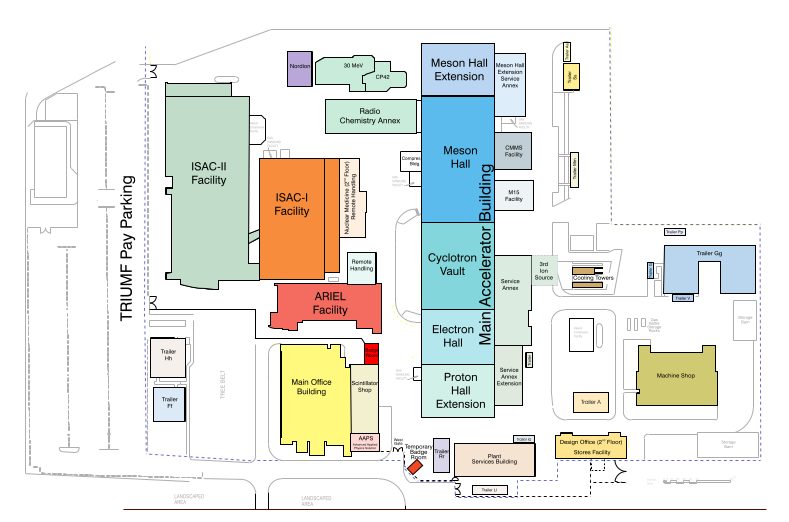
\includegraphics[width=1.0\textwidth]{sitemap.png}
  \caption{A map of TRIUMF. The UCN facility is located at the Meson
    Hall area shown in Blue.}
  \label{fig:sitemap}
\end{figure}

The unique feature of the UCN source at TRIUMF is the combination of
spallation neutrons and superfluid helium for UCN production. The
important elements of the UCN facility at TRIUMF are presented below.
%%%%%%%%%%%%%%%%%%%%%%%%%%%%%

%%%%%%%%%%%%%%%%%%%%%%%%%%%%%
\section{UCN Beam Line~(BL1U)}
TRIUMF produces negatively charged hydrogen ions from an ion
source. These ions are then accelerated in the 520~Mev cyclotron in an
outward spiral trajectory. A thin graphite stripper foil removes the
electrons from the hydrogen ion while protons can pass through. The
proton, because it is a positively charged particle, is deflected in
the outward direction due to the magnetic field and is directed to a
proton beam line. The cyclotron has three independent extraction
probes with various sizes of foils to provide protons to up to three
beam lines~(BL) simultaneously~(see Fig.~\ref{fig:cyclotron}).

\begin{figure}[h!]
  \centering
  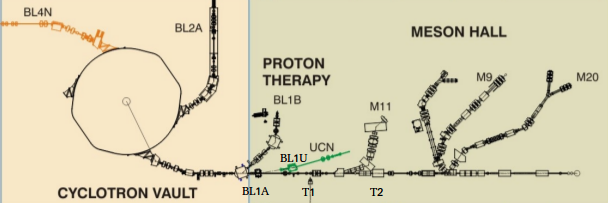
\includegraphics[width=0.8\textwidth]{cyclotron.png}
  \caption{TRIUMF cyclotron and the three beam lines.}
  \label{fig:sitemap}
\end{figure}


The 120~$\mu$A beam (BL1A) enters the Meson Hall, routinely delivers
protons at 480~MeV to two target systems: T1 and T2 for the $\mu$SR
experimental channels. Beam line 1B~(BL1B) separates off BL1 at the
edge of the cyclotron vault and provides international users with the
Proton Irradiation Facility (PIF), which mimics space radiation for
testing computer chips.  The new BL1U provides beam to the UCN
source. BL2A provides 480~MeV proton beams for the targets that
produce exotic ion beams for a host of experiments in ISAC.


The microstructure of BL1A is in pulses with approximately 1~ms
periods of beam followed by a 50-100~$\mu$s periods of no beam.  This
is shown in Fig.~(\ref{fig:bl1u})~\cite{Nick_thesis}.  A kicker magnet
and the septum magnet kick away 1/3 of the beam from BL1A to BL1U and
transport it to a conventional dipole~(bender) magnet~(See
Fig.~\ref{fig:magnets}).

\begin{figure}[h!]
  \centering
  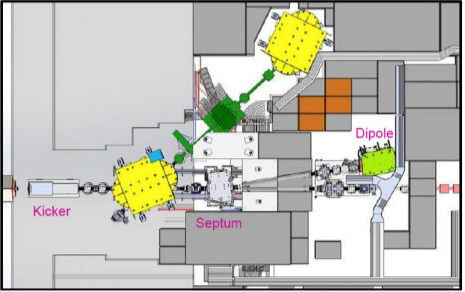
\includegraphics[width=0.9\textwidth]{magnets.png}
  \caption{The kicker, septum and dipole (bender) magnets define the
    front two sections of BL1U.}
  \label{fig:magnets}
\end{figure}
The vertical UCN cryostat is sitting above the tungsten target and is
designed for a maximum of 40~$\mu$A beam on target. As a result, only
one third of the beam can go to the UCN experimental area and the rest
is shared with other users.

\begin{figure}[h!]
  \centering
  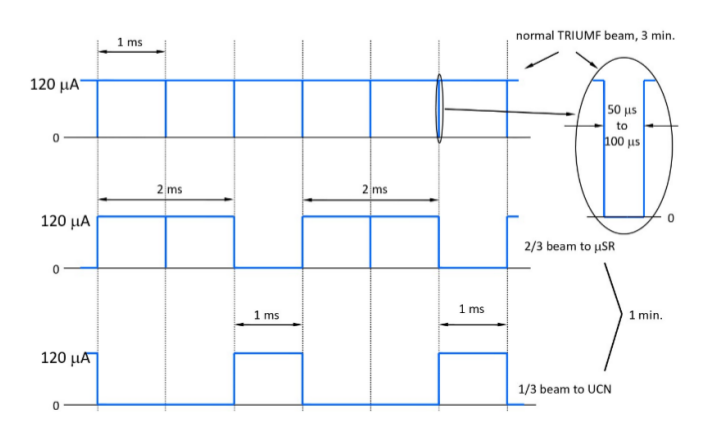
\includegraphics[width=0.9\textwidth]{bl1u.png}
  \caption{UCN beam structure. The top graph shows the 120~$\mu$A BL1A
    in 1~ms period of beam followed by a 50-100~$\mu$s of no
    beam. The middle graph shows the same beam line when the kicker
    magnet is on. The bottom graph shows the 1/3 of the beam that goes
    to the UCN area.}
  \label{fig:bl1u}
\end{figure}

After the bender magnet, the beam then passes through a cored
shielding block and reaches the two quadrupole magnets providing the
final focus of the beam onto a 12~cm thick tungsten spallation target.
The target is located inside a hermetically-sealed target crypt, which
also envelops the beam line exit window that defines the end of BL1U.
Upstream of the beam line window, there is a collimator to reduce the
halo from the proton beam, as well as to help reduce the amount of
neutrons and photons streaming back into the beam line from the target
region~(the collimator also increases the impedance for the passage of
gas arising from any target or window failure, to allow time for the
cyclotron fast valves to close). This last part of the beam line also
contains a variety of beam position and current monitors. The
spallation target and UCN source, located downstream of the beam
line-exit window, are enclosed in a large shielding
pyramid~Fig~\ref{fig:pyramid}.
\begin{figure}[h!]
  \centering
  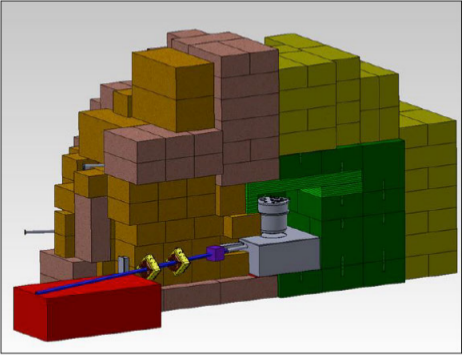
\includegraphics[width=0.8\textwidth]{pyramid.png}
  \caption{Two quadrupole magnets which focus the proton beam onto a
    12~cm thick tungsten spallation target, located inside a
    hermetically-sealed target crypt. Also shown is the UCN shielding
    pyramid, which encases both the spallation target and the UCN
    source, and is designed to meet the dose rate requirements
    specified by the TRIUMF Safety Group.}
  \label{fig:pyramid}
\end{figure}

\section{Tungsten Spallation Target\label{sec:target}}
The spallation target is located at the downstream end of BL1U. The
UCN spallation target comprises a series of rectangular blocks, adding
up to roughly one stopping length~(11~cm) of tungsten, with a
cross-section of $\sim6 \times 8$~cm$^2$~(see
Fig.~\ref{fig:target}). This geometry is very similar to~(and
motivated by) the neutron spallation target design used at KEK (KENS
facility)~\cite{kawai2001fabrication}. The target requires a support
and cooling system, and is designed to allow for remote-handling and
ease of servicing. The target-cooling and remote-handling systems are
designed for an instantaneous proton current of 40~$\mu$A~(10~$\mu$A
time-averaged).
\begin{figure}[h!]
  \centering
  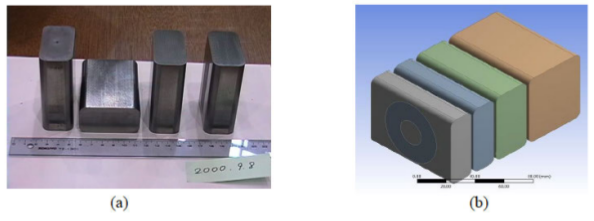
\includegraphics[width=0.8\textwidth]{target.png}
  \caption{(a) Tungsten Target Blocks from the spallation target at
    KEK. The target blocks are plated with tantalum. (b) Present
    design for the tungsten spallation target at the TRIUMF UCN
    facility. The target blocks have a cross-section of
    $5.7 \times 7.8$~cm$^2$ , and thicknesses of 2.0, 2.0, 3.0, and
    5.0~cm, respectively.}
  \label{fig:target}
\end{figure}
The target is being water-cooled. A coating of tantalum prevents
corrosion by the water cooling system. An extraction system allows to
exchange the target when necessary.

%\section{Radiation Sheilding}
% I am not sure if there is anything specific about shielding to
% say. It comes with moderators and when I show the figures of the
% experimental area it will be mentioned.

%%%%%%%%%%%%%%%%%%%%%%%%%%%%%%%%%%%%%%%%%%%%%%%%%%%
%%% JUST TALKING ABOUT THE SETUP
%%%%%%%%%%%%%%%%%%%%%%%%%%%%%%%%%%%%%%%%%%%%%%%%%%%
\section{Vertical UCN Source at TRIUMF\label{sec:vertical_source}}
Neutrons are produced through the spallation process by hitting a
Tungsten target by the proton beam. Spallation is refered
to a nuclear reaction where high energy particles interact with atomic
nucleus. This process creates many high energy neutrons and background
radiation. The target is surrounded by several blocks of lead and
graphite. The fast neutrons are reflected and moderated down and enter
the warm D$_2$O moderator at room temperature~(300~K) and become
thermal neutrons with an energy of 0.025~eV and the speed of 2.2~km/s.
Iced heavy water at 10~K is used as a cold moderator. After passing
through the warm D$_2$O, thermal neutrons enter the the cold moderator
and become cold neutrons. These neutrons have the speed of several
hundreds of meter per second.  UCN are produced when the slow neutrons
enter the isotopically pure superfluid helium at 0.84 to 0.92~K as a
result of phonon transitions inside the superfluid helium as discussed
in section~\ref{sec:ucn_with_heII}.

The schematic of the vertical source is shown in
Fig.~\ref{fig:source}.  The neutron moderators and the helium
circulation system are explained below.


\begin{figure}[h!]
  \centering
  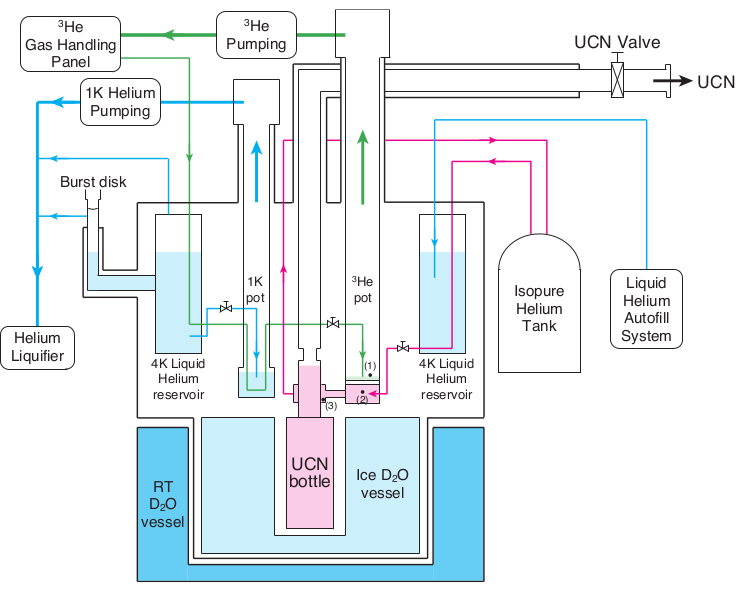
\includegraphics[width=0.9\textwidth]{vertical_source.png}
  \caption{Schematic diagram of the vertial UCN source at
    TRIUMF. Spallation neutrons are moderated in warm D$_2$O vessel
    and become cold neutrons in Iced D$_2$O. The cold neutrons then
    enter the superfluid helium bottle where they become UCN by phonon
    excitations in the superfluid. The isotopically pure superfluid
    helium is cooled down to below 1~K via a $^3$He pot. The $^3$He
    pot is cooled down to 0.7~K via 1~K pot and further pumping. The
    detailed explanation is available in the text. }
  \label{fig:source}
\end{figure}


\subsection{Neutron D$_2$O Moderators}
Deuterium is an isotope of hydrogen which has one proton and one
neutron in the nucleus and it has a lower probability to absorb
neutrons. As a result heavy water is used as a neutron moderator. The
warm D$_2$O moderator to create thermal neutrons from spallation
neutrons is at room temperature. However the cold moderator for the
production of cold neutrons is at much lower
temperature~($\sim$~10~K).

\subsubsection{D$_2$O Solidification}
The Iced D$_2$O vessel has a capacity of 100~L. About 14~L of liquid
D$_2$O is injected to the vessel initially. This is followed by adding 11~L of
D$_2$O to the vessel over 8 times.  After filling up the vessel,
Gifford McMahon refrigerators solidify the heavy water and further
cool it down to 20~K. The process of icing the heavy water takes about
6 days and cooling it down to 20~k takes another 7 days.

%%%%%%%%%%%%%%%%%%%%%%%%%%%%%%%%%%%%%%%%%%%%%%%%%%%
% This is where I left off and where I should start
% again on Monday

\subsection{Helium Circulation and Superfluid Helium Condensation}
The helium circulation and the condensation of the superfluid helium
could be started once the temperature of D$_2$O is as low as 10~K. The
stages towars superfluid helium condensation is presented below. The
full operation and desing detail are available in
Ref.~\cite{matsumiya_thesis}.

\subsubsection{4 Kelvin Reservoir}
The first step of the helium circulation is to fill up the helium
reservoir with the commercially available 4.2~K helium. The full
capacity of the helium reservoir is 50~L. In the 2017 experimental
run, the TUCAN collaboration used a labview program to automatically
fill up the reservoir using a 500~L dewar of 4.2~K helium. This was
refered to as the {\it{stationary dewar}}. This way, it is possible to
set the minimum and maximum levels of the available helium. The helium
levels were measured by two level meters and two flow meteres. The DAQ
system and sensor positions are described in Sec.~\ref{sec:DAQ}.  The
stationary dewar was filled up with 350~L dewars~({\it{transport
    dewar}}) of 4~K helium from the meson hall liquifier. The helium
autofill system is shown in Fig.~\ref{fig:ucnarea}.

\begin{figure}[h!]
  \centering
  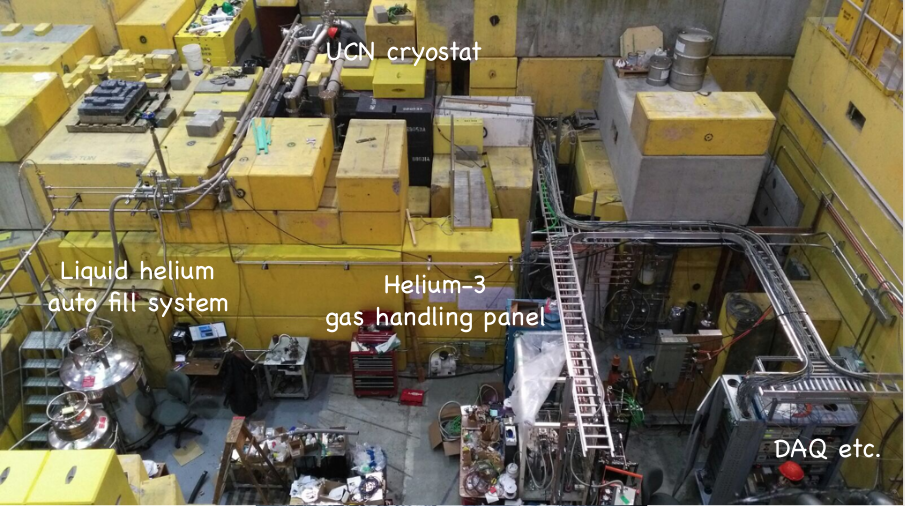
\includegraphics[width=0.9\textwidth]{ucnarea.png}
  \caption{A photograph of the UCN experimental area during the mini
    shutdown in October 2017. The location of some experimental parts
    are shown via labels. The yellow concrete blocks are blocking the
    radiation during beam on target. The UCN vertical cryostat could
    be seen because of the removal of the shield. }
  \label{fig:ucnarea}
\end{figure}

Fig.~\ref{fig:4kfilling} shows the 5 filling cycles of the 4~K
reservoir on April 22 2017 during the first cool down test. The liquid
helium transfer starts once the liquid level in the 4~K reservoir
reaches 20\%. Once the transfer starts, the liquid level starts to
decrease with a sharper slope. The reason for this behaviour is
introducing heat load to the reservoir. It takes some time to cool
down the transfer line from the stationary dewar to the reservoir and
the warm liquid helium causes a boil off in the 4~K reservoir. The
boiled off helium goes through the recovery line to the liquifier. The
liquid helium transfer stops once the 4~K reservoir is filled to about
60\%.

\begin{figure}[h!]
  \centering
  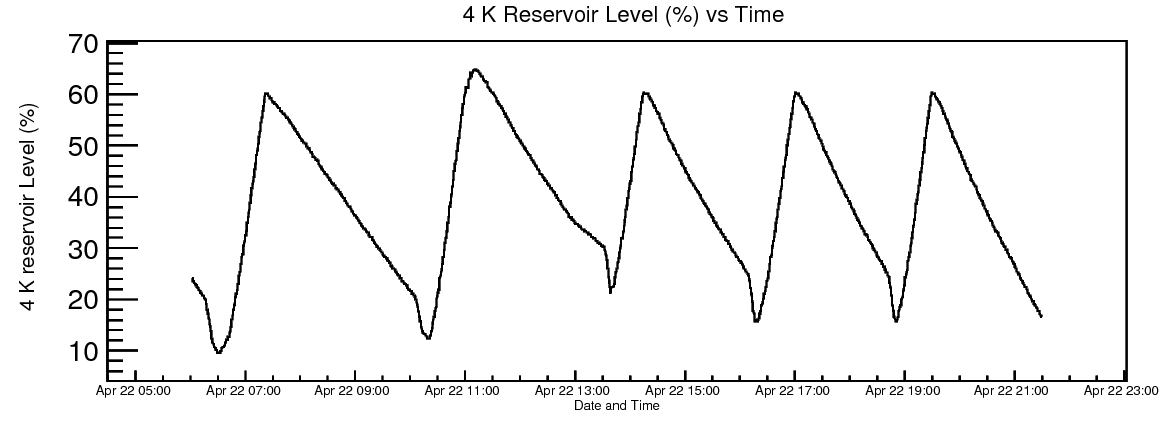
\includegraphics[width=1.0\textwidth]{april_4kfilling.png}
  \caption{The 4~K reservoir filling during the cool down test in April 2017.}
  \label{fig:4kfilling}
\end{figure}
The efficiency of each transfer from the stationary dewar to the 4~K
reservoir was about 40\% to 60\% on average.

\subsubsection{1 Kelvin Pot}
The 4.2~K liquid helium in the helium reservoir is transported to a
pot called {\it{1~K pot}}. The flow rate of the transported liquid
helium is controlled by a needle valve. The 1~K pot is always pumped
by a pumping system to cool the 4.2~K helium down to about 1.4~K. The
level of helium in the 1~K pot is measured by a liquid level
meter. The maximum level of the 1.4 K liquid helium is about 15~cm. At
this level, the volume of the 1.4~K liquid helium is about 1.3~L.


\subsubsection{$^3$He Pot}
Once the 1~K pot is ready the $^3$He circulation starts to condense
into the {\it{$^3$He pot}}. To start, the valve of the $^3$He
reservoir is opened. A vaccum pump compresses the $^3$He gas. The
$^3$He gas is then purified by a room temperature and a cold purifier
and enters the 4~K reservoir to be precooled. The further cooling down
to 1~K and condensation happen via the 1~K pot. The liquid $^3$He is
then transported to $^3$He pot and further cooled down to 0.7~K via
pumping. The evaporated $^3$He is pumped out and goes through an oil
filter and goes back to the beginning point of the circulation.

\subsubsection{Isopure Helium}
After filling the $^3$He pot with 0.7~K liquid $^3$He, the
condensation of isotopically pure~(isopure) superfluid helium
starts. The isopure helium has much less $^3$He than $^4$He~(less than
$10^{-10}$).  Even though the natural abundance of $^3$He is
$1.37 \times 10^{-6}$ in the atmosphere, this value is still large
because of the large neutron absorption cross section of $^3$He. The
existence of $^3$He causes the UCN storage lifetime to decrease~(see
Sec.~\ref{sec:basic_idea}).

The isopure helium is stored in the {\it{isopure helium tank}} shown
in Fig.~\ref{fig:source}. Before entering the cryostat, the
isopure helium goes through a purifier. The purifier is composed of
low temperature charcoals cooled by LN$_2$.  The isopure He is
precooled in the 4~K reservoir and goes into the heat exchange pot
attached to the bottom of the $^3$He cryostat. The bottom of the
$^3$He cryostat and the top of the heat exchange pot is connected via
the copper heat exchanger. The isopure He in the heat exchange pot is
cooled by the 0.7~K liquid $^3$He via the Cu heat exchanger and
becomes He-II. The condensed He-II fills the He-II bottle with a
volume of 8.5~L and gets cooled down to $\sim$~0.83~K.




\section{Data Acquisition System\label{sec:DAQ}}
The TUCAN UCN DAQ system accumulates data from different devices and
integrates them into a MIDAS file.

For the 2017 data acquisition, almost all the sensors such as
temperature sensors, flow meteres, pressure gaugas and {\it{etc.}}
were connected to a Programmable Logic Controller~(PLC).  The PLC
receives information from the connected sensors or input devices,
processes the data, and triggers outputs based on pre-programmed
parameters.  Depending on the inputs and outputs, a PLC can monitor
and record data, automatically start and stop processes, generate
alarms based on the applied limits, and more. A picture of the PLC is
shown in Fig.~\ref{fig:PLC}.

\begin{figure}[h!]
  \centering
  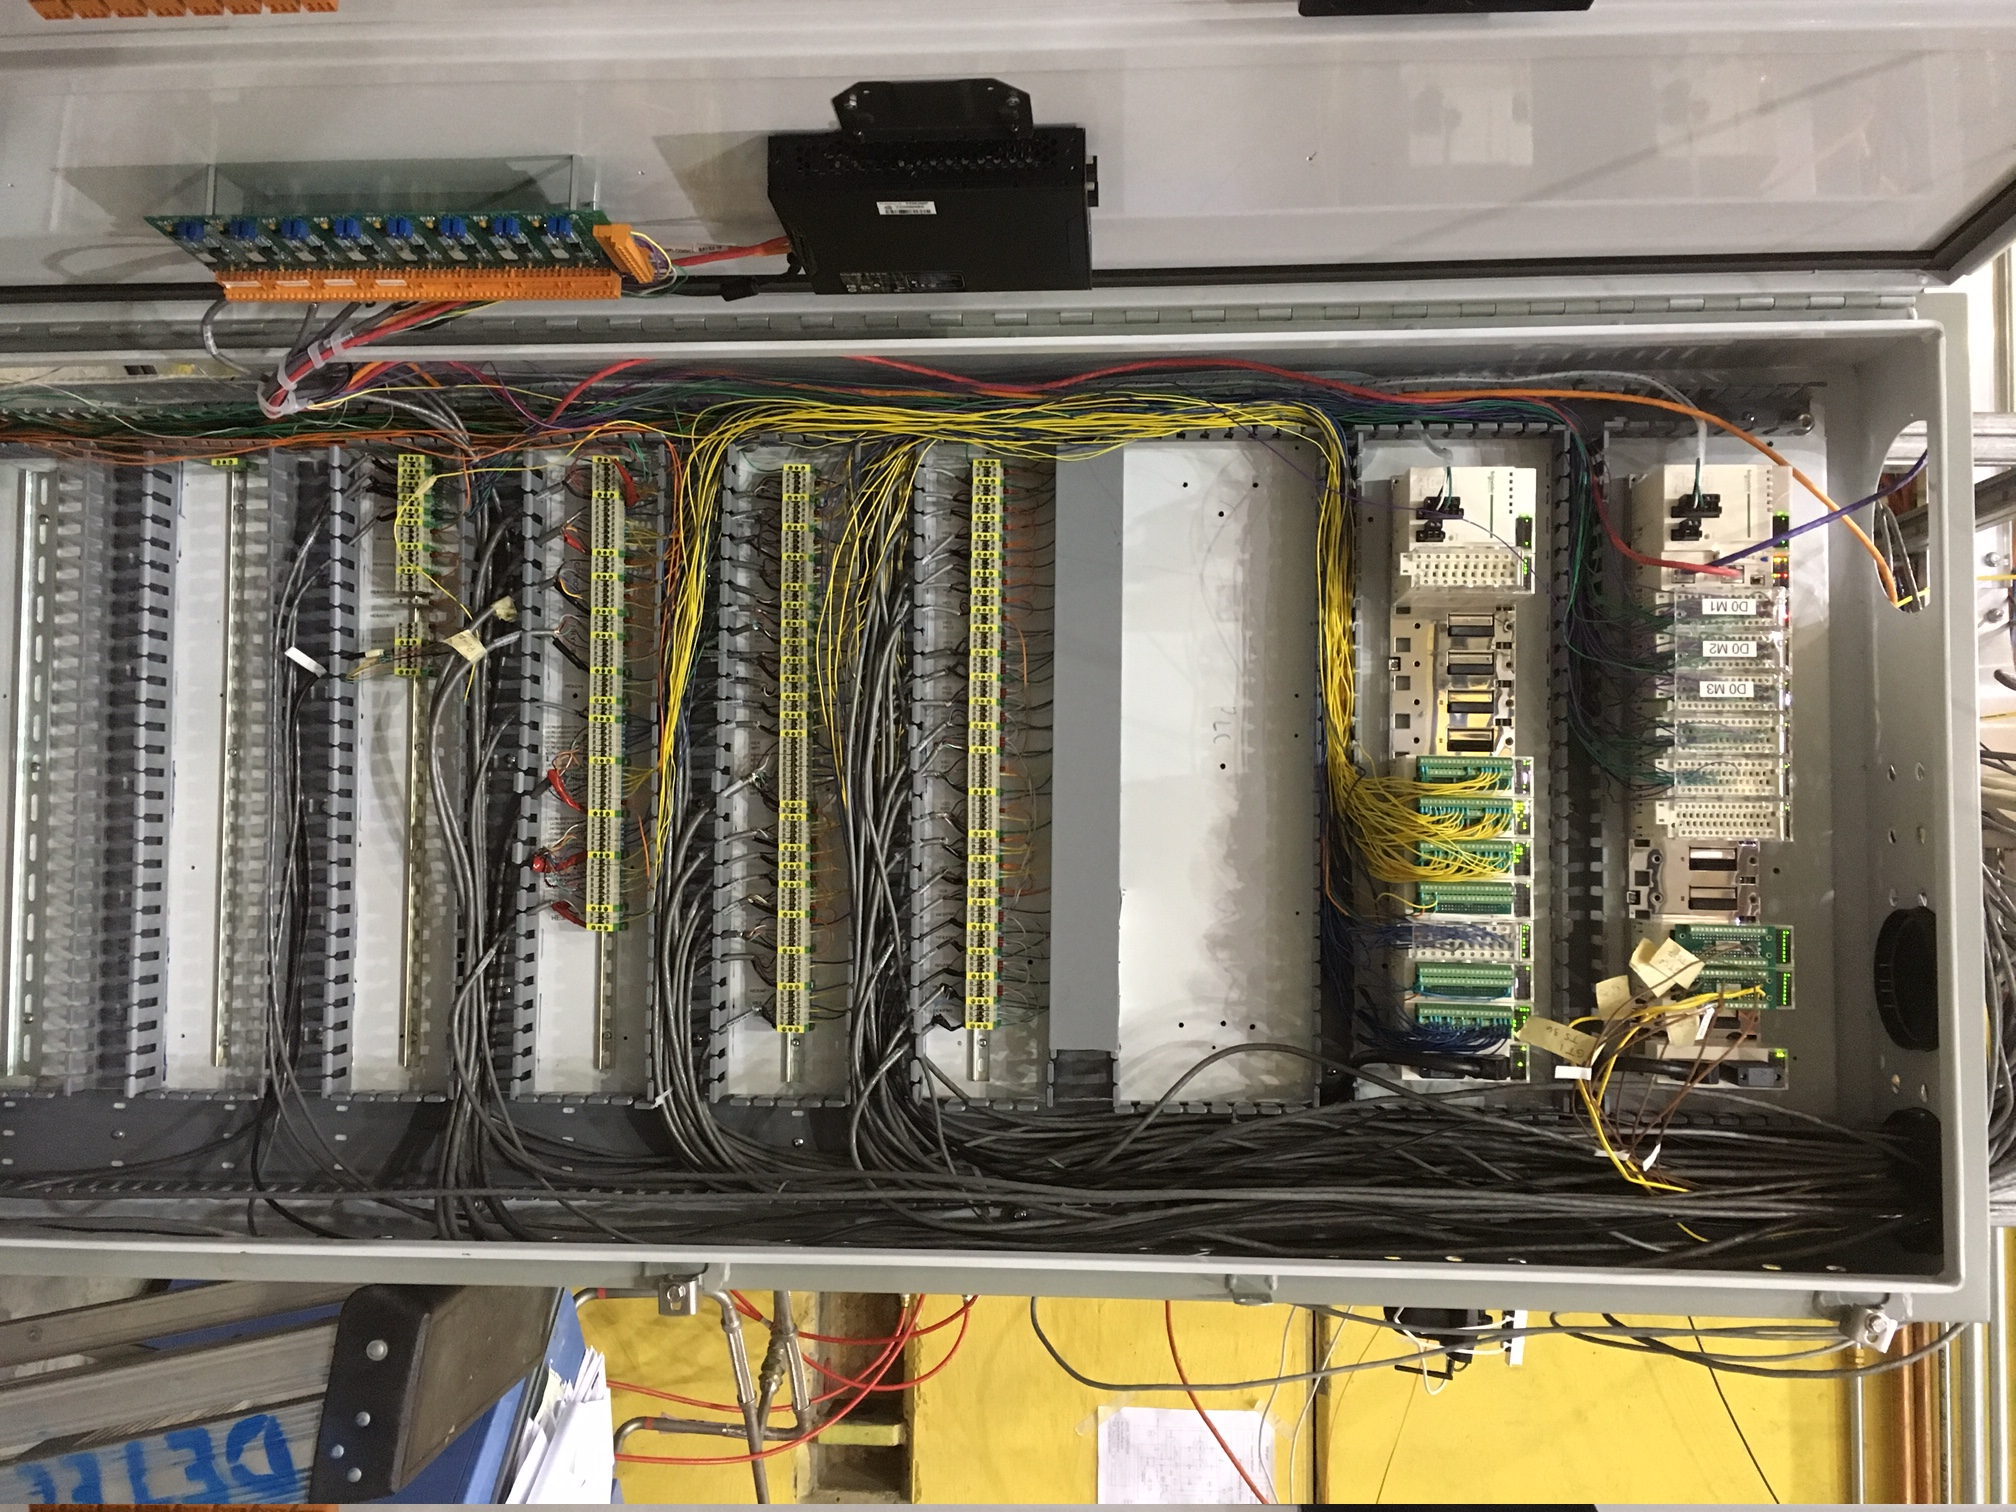
\includegraphics[width=0.8\textwidth, angle = 90]{PLC.JPG}
  \caption{A photograph of the PLC in the meson hall. The grey blocks
    are used to connec the signal from the devices to the computing
    moduels. The first two rows are where the modules are
    located. Each sensor is connected to a specific terminal on a
    specific module. The bottom row is where the power supplies and the
    fuses are positioned. {\bf{insert a new photo}} }
  \label{fig:PLC}
\end{figure}
The communication between the PLC and the screen is handled by EPICS.
The EPICS screen defines the user interface for the controls. It
provides readouts of variables, indications of device status, and
various user input controls for turning devices on/off, resetting
devices, etc. The screen shows the approximate physical layout of the
apparatus being controlled, with each device and its controls placed
in its actual location. The colours of the devices are used to
indicate their current status~\cite{Sean_manual}. Fig.~\ref{fig:epics}
shows the thermal EPICS screen for the TUCAN vertical UCN source
during the November 2017 experimental run. The gas flow screen~(not
shown, very similar to the thermal screen) is intended to contain all
the information about pressures, flows, levels, and controls for pumps and
valves.

\begin{figure}[h!]
  \centering
  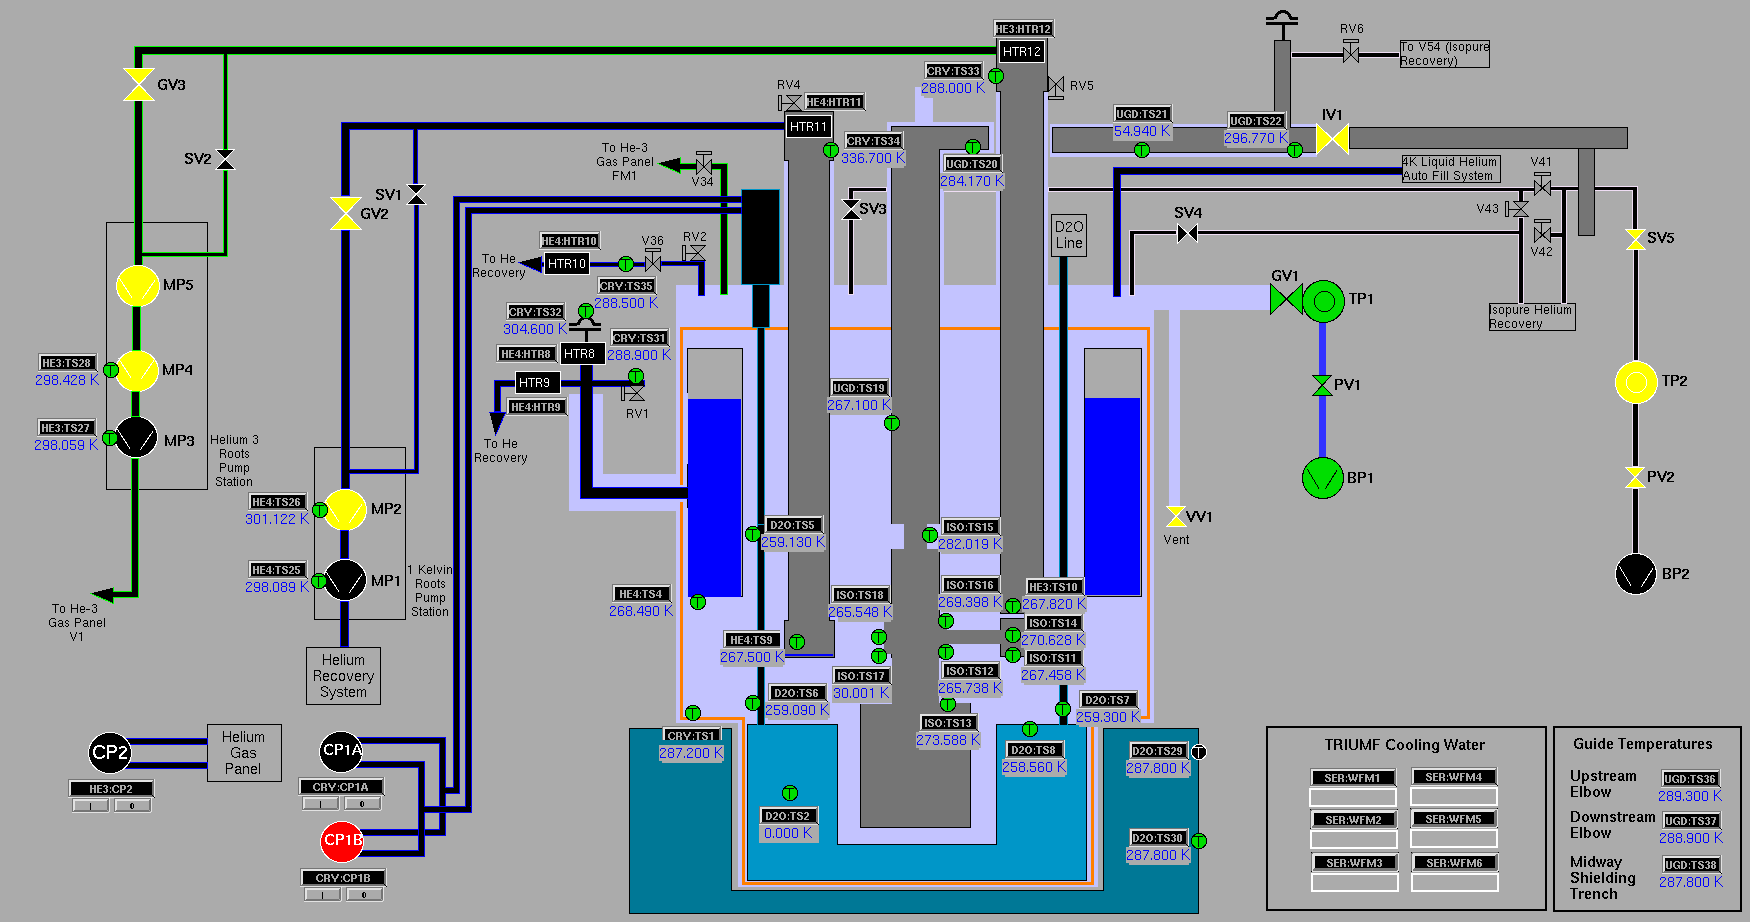
\includegraphics[width=1.0\textwidth]{epics.png}
  \caption{EPICS thermal screen. The approximate location of each
    temperature sensor is shown.The thermal screen is intended to
    contain all information about temperatures, and controls for
    compressors and heaters. }
  \label{fig:epics}
\end{figure}

MIDAS is a modern data acquisition system developed at PSI and TRIUMF
written in C/C++ which runs on all operating systems. MIDAS logs data
in two different ways: History logging where some data is saved
periodically~(every 1-10~s) and can be plotted from history page and
file logging where all data is saved to MIDAS file to be analyzed
later. The TUCAN MIDAS DAQ has a web interface shown in
Fig.~\ref{fig:midas}. The green color indicates that the equipment
frontend is running. Each run can be started by pressing the button at
the top section.

\begin{figure}[h!]
  \centering
  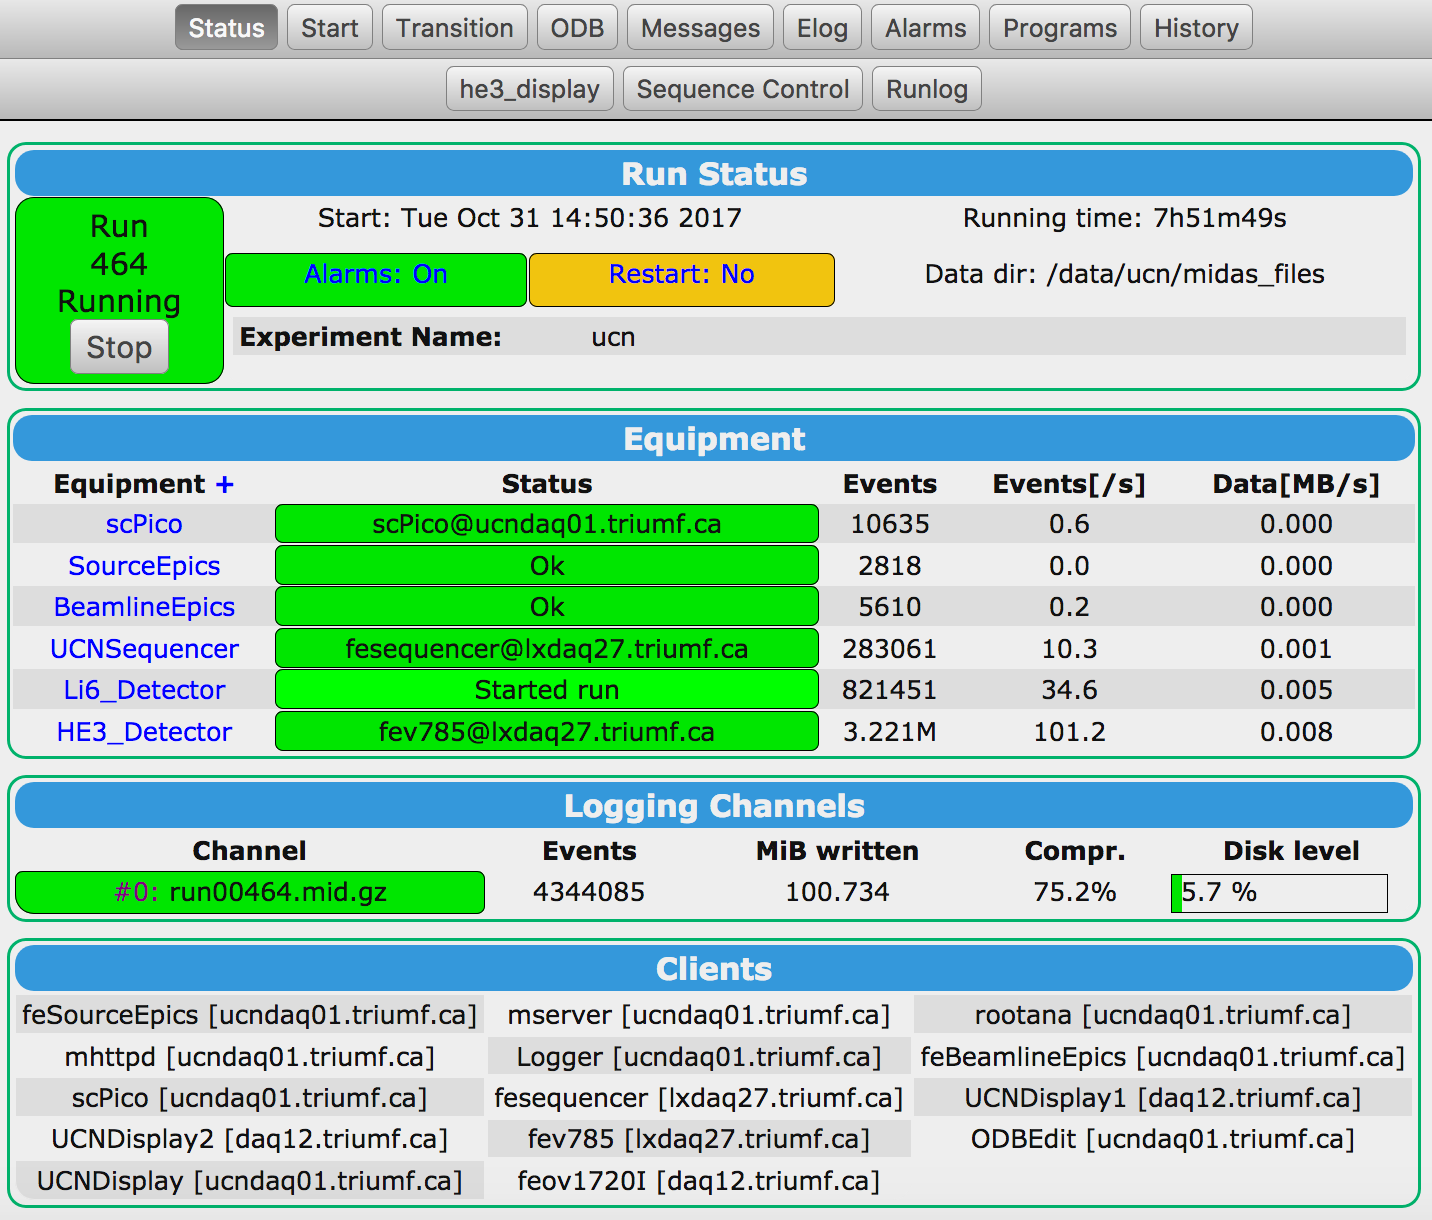
\includegraphics[width=0.8\textwidth]{midas.png}
  \caption{TUCAN MIDAS web interface }
  \label{fig:midas}
\end{figure}

For the 2017 experimental run, each expriment had a unique MIDAS
number. The MIDAS files were then converted to ROOT files for data
analysis. The result of the analysis is presented in
Chapter~\ref{chap:UCNresult}.

\section{UCN Detectors\label{sec:detectors}}
For the TUCAN experimental runs in 2017, a $^6$Li and a $^3$He
detector were used. The main reason for this was to check the
consistency of the result and the performance of each detector. The
brief description of each detector is available below.

\subsection{$^6$Li Detector\label{sec:Li6detector}}
The main detector used during the UCN measurements~(See
Chapter~\ref{chap:UCNresult}) is a $^6\mathrm{Li}$ glass based scintillator
detector designed and built at the University of Winnipeg for the
TUCAN nEDM experiment at
TRIUMF~\cite{jamieson2017characterization}. Since $^6\mathrm{Li}$ has a high
neutron capture cross-section~(order of $10^5$ bn) at UCN energies,
the scintillator glass is doped with it. The charged particles in the
reaction
\begin{equation}
^6Li + n \rightarrow \alpha (2.05~\mathrm{MeV}) + t (2.73~\mathrm{MeV})
\end{equation}
are detected. To reduce the effect of $\alpha$ or triton escaping the
glass, a layer of 60~$\mu$m thick depleted $^6\mathrm{Li}$ glass (GS30), on top
of a layer of 120~$\mu$m thick dopped $^6\mathrm{Li}$ (GS20) were optically
bonded. This design allows the resultant particles to deposit all of
their energy within the scintillating
glass. Table~\ref{tab:scintillator} shows the content and density of
those $^6\mathrm{Li}$ scintillators.

\begin{table}[h!]
  \centering
  \label{tab:scintillator}
  \begin{tabular}{|c|c|c|}
    \hline
    Scintillator & GS20~($^6\mathrm{Li}$ Enriched) & GS30~( $^6\mathrm{Li}$ depleted) \\
    \hline
    Total Li content (\%) & 6.6 & 6.6 \\
    \hline
    $^6\mathrm{Li}$ fraction (\%) & 95 & 0.01 \\
    \hline
    $^6\mathrm{Li}$ desity~(cm$^{-3}$) & $1.716 \times 10^{22}$ & $1.806 \times 10^{18}$ \\
    \hline
  \end{tabular}
  \caption{Properties of the glass scintillators}
\end{table}


Making the scintillating Li glass as thin as possible reduces the
sensitivity to $\gamma$-ray scintillating backgrounds and and thermal
neutron captures. The mean range of the $\alpha$ is 5.3~$\mu$m and the
mean range of the triton is 34.7~$\mu$m. This means that if the
thickness of the scintillator is less than 50~$\mu$m, the resultant
particles escape before stopping which gives rise to an efficiency
loss.  In order to handle high UCN rates of up to \~1~MHz, the
$^6\mathrm{Li}$ detector face is segmented into 9 tiles~(See
Fig.~\ref{fig:Li6detector}). The scintillation light is then guided
through ultra-violet transmitting acrylic light-guide to its
corresponding Photomultiplier Tube~(PMT) outside the vaccum region of
the detector.

\begin{figure}[h]
  \centering
  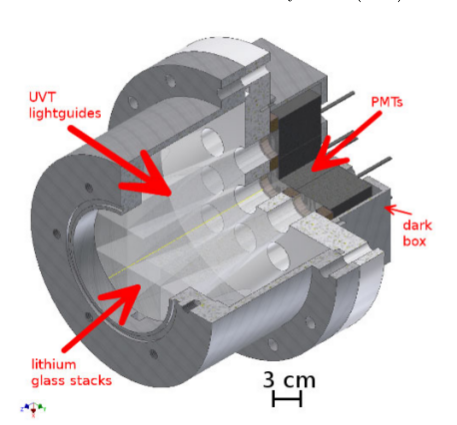
\includegraphics[width=0.5\textwidth]{Li6detector.png}
  \caption{3D drawing of the $^6$Li detector and its enclosure. The
    enclosure is made of Al, and the rim of the adapter flange which
    UCN can hit is ccoated with 1~$\mu$m Ni by thermal evaporation. }
  \label{fig:Li6detector}
\end{figure}

The data acquisition with this detector includes a CAEN V1720
digitizer which has a Pulse-Shape Discrimination~(PSD) firmware that
triggers on pulses below a certain threshold for each channel. Every
4~ns the digitizer samples the waveform which is then digitized to a
voltage on a 2~V scale into an ADC value between 0 and 4096. Each
channel of the digitizer sends a trigger whenever the number of counts
in the ADC goes below a certain baseline~(pedestal) value. The PSD
calculates the sum of the signal below the baseline for two time
windows: $t_s = 40$~ns (short gate) and $t_L = 200$~ns~(long
gate). The short gate is chosen in a way to contain all of the charge
for the $\gamma$-ray interactions in the light-guide. The ADC sum for
during the long gate below the baseline is calle $Q_L$~(read charge
long) and for during the short gate below the baseline is called
$Q_S$. Charge long has the total charge deposti for the neutron
capture events. The PSD value is defined as
\begin{equation}
  \label{eq:psd}
  \mathrm{PSD} = \frac{\left( Q_L - Q_S\right)}{Q_L}
\end{equation}  
which is the amount of charge in the tail of an event.

Jamieson {\it{et al.}} showed that the absolute efficiency of this
detector is $89.7^{+1.3}_{-1.9}$~\% with a background contamination of
$0.3 \pm 0.1$~\%~\cite{jamieson2017characterization}. The detector is
stable at the 0.06~\% level or better, and that the variation in the
efficiency between the detector tiles is less than 5~\%.
\subsection{$^3$He Detector}

The $^3$He detector used for the data acquisition is a Dunia-10 type
which was shipped from RCNP.  $^3$He provides an effective neutron
detector material for neutron detection by absorbing neutrons via the
following reaction

\begin{equation}
  \label{eqn:he3}
n + ^3\mathrm{He} \rightarrow p + t + 674~\mathrm{keV}.
\end{equation}

Before the start of the experiment, the $^3$He detector was tested
with an AmBe source and it showed consistent result with what was
observed at RCNP. The detector was surrounded with parafin blocks to
moderate the neutrons~(see Fig.~\ref{fig:he3detector}.

\begin{figure}[h]
  \centering
  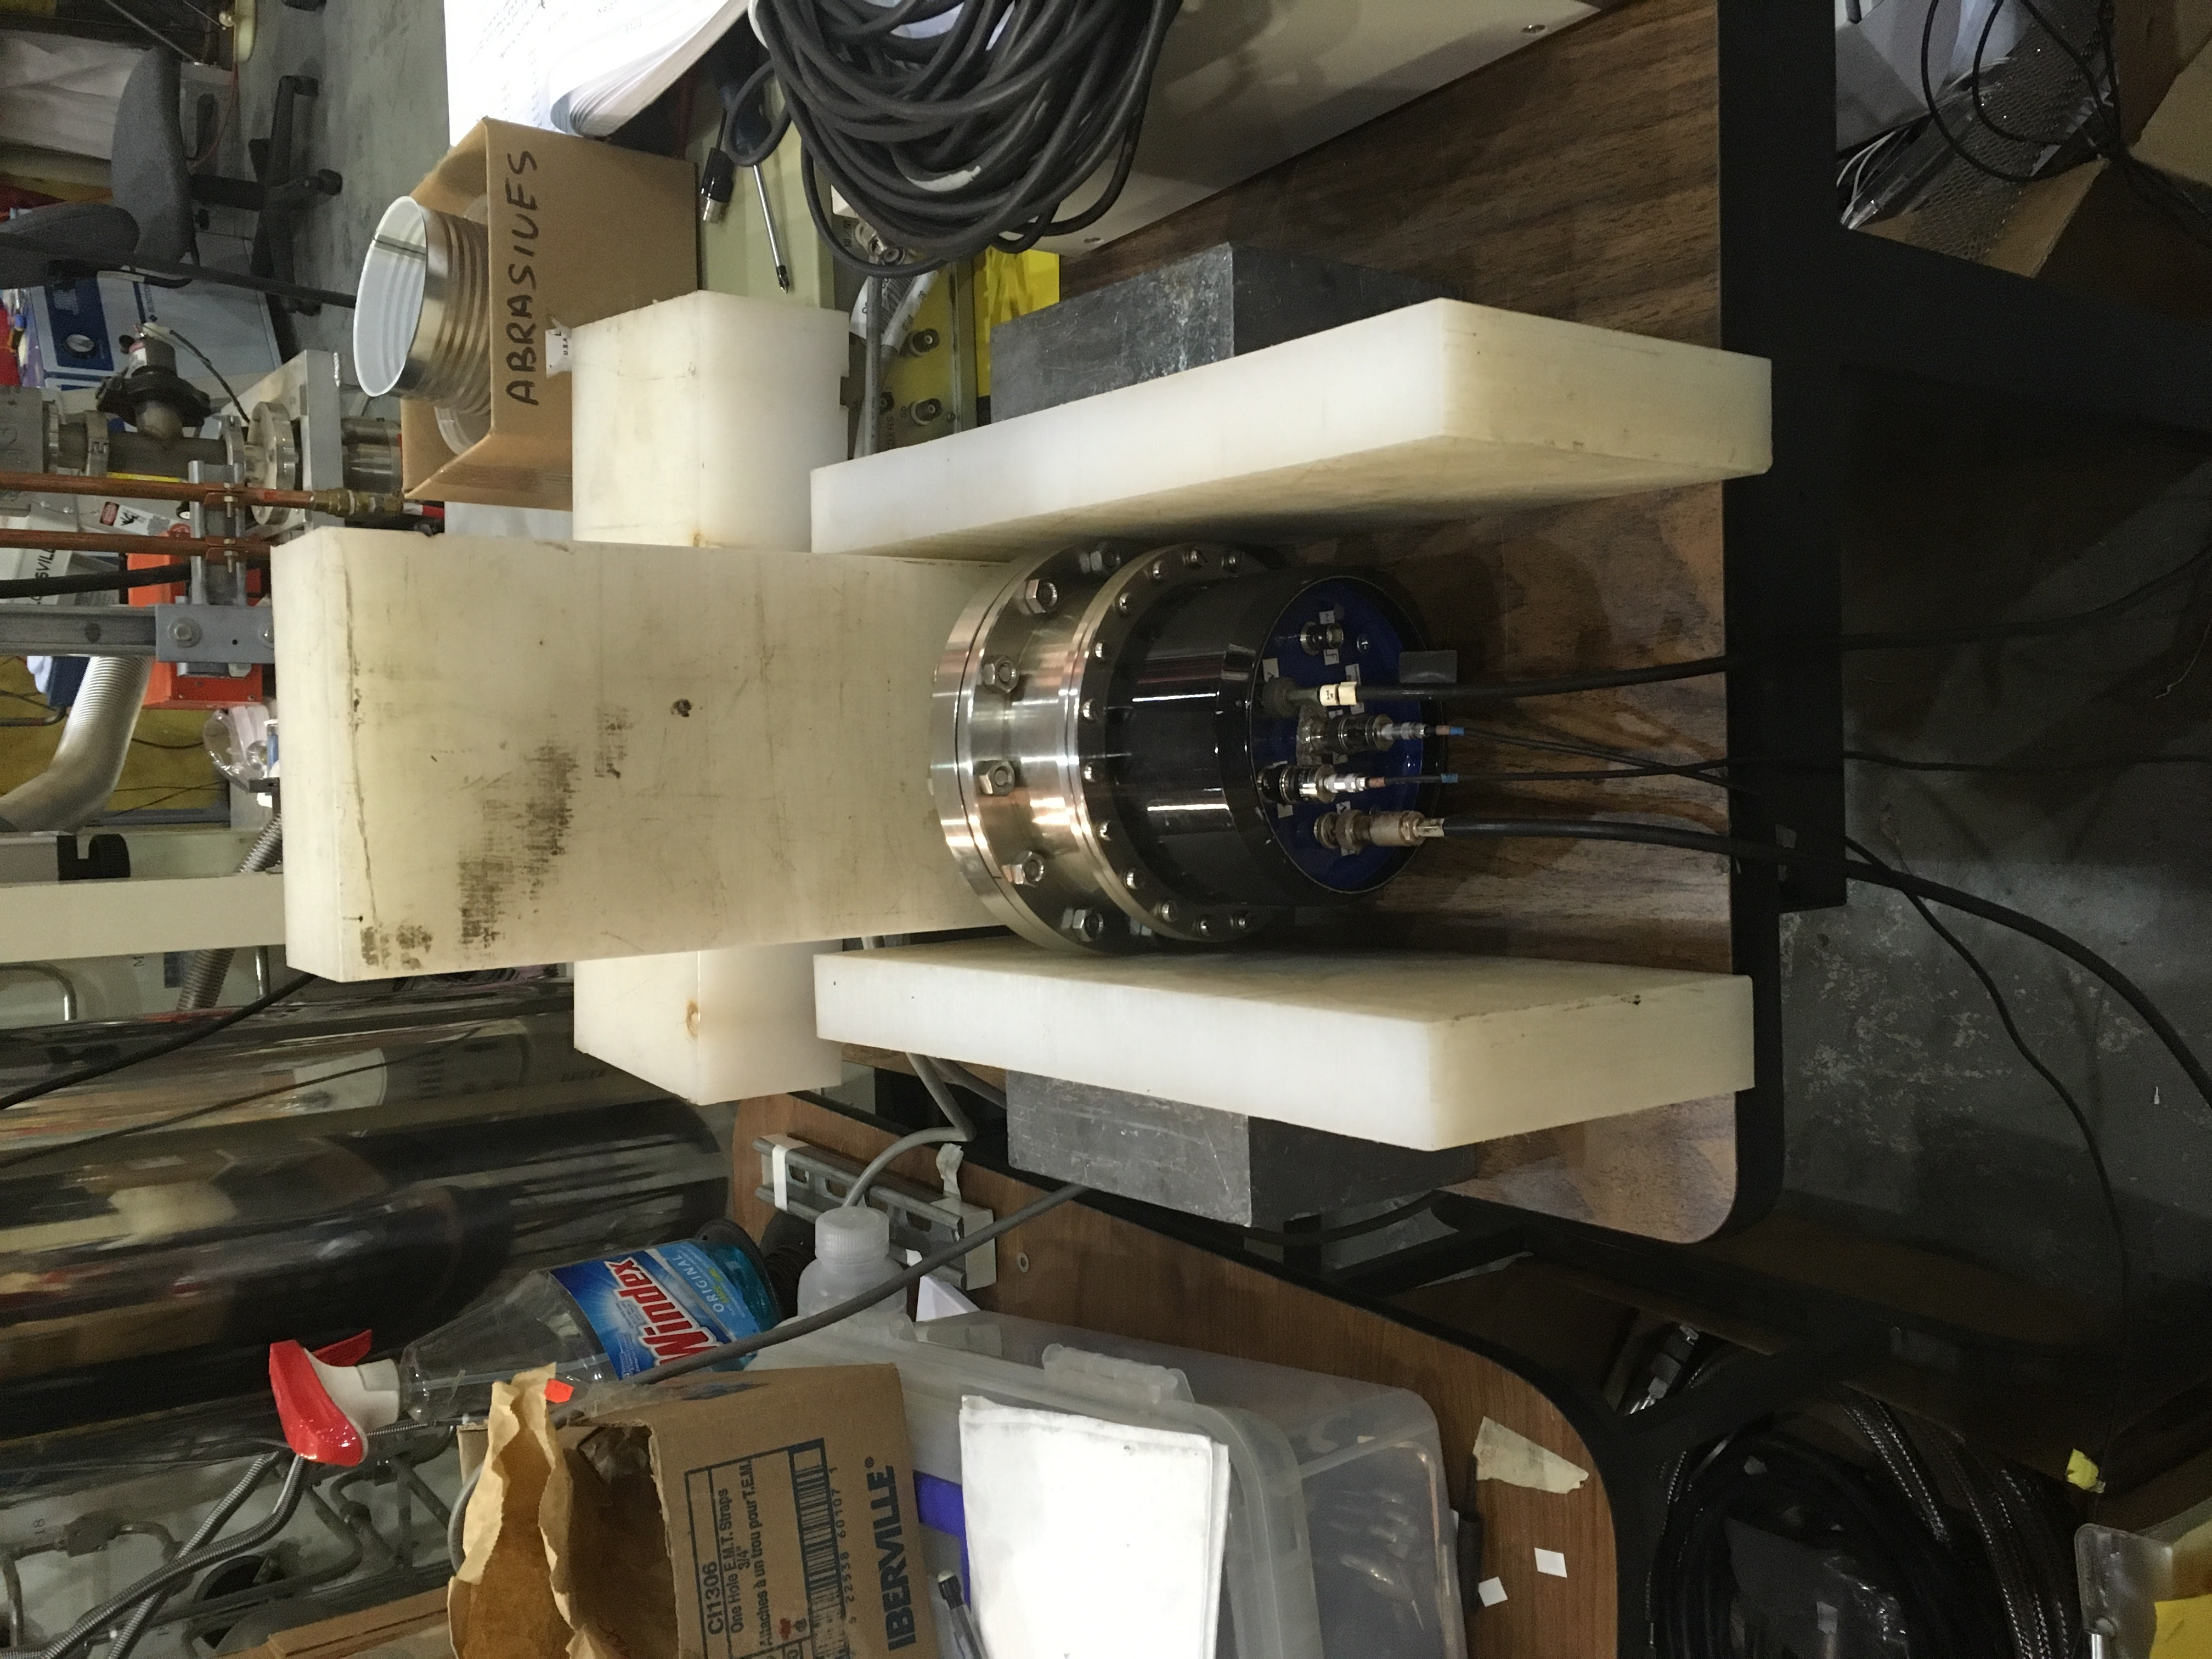
\includegraphics[width=0.5\textwidth, angle = 270]{he3detector.png}
  \caption{$^3$He detector and parafin blocks for neutron
    moderation.}
  \label{fig:Li6detector}
\end{figure}

More detail about the $^3$He detector could be found in
Ref.~\cite{matsumiya_thesis}.
% The result of the comparison between the $^3$He and $^6$Li detectors
% are available in Sec.~\ref{sec:detector_comparison}.

%\begin{description}
%\item{An intro to whatever goes into this chapter}

%\item{Start by showing a nice drawing and then talk about each
 % componet of the facility:}
  
%\item{about proton beam that we get, the magnets and basically how the
%  beam reaches the target and how it looks like (Where can I get this
%  information? Is it written somewhere?)}
  
%\item{A short introduction to say the stages of UCN production and why
%  we need the vertical cryostat (Link to the next stage)}
  
%\item{It also has to be mention that it is the same vertical sourcse
%  as was used at the RCNP and some modifications were made to meet the
%  requirements at triumf. (Where can I find what modifications were
%  made?) Agian this has to be just as a link to the next chapter(maybe?)}
  
%\item{The target and shielding (with pictures?), only a few
%  paragraphs}
  
%\item{Moderation: D2O system (I can use Ryohei's thesis I guess)}
  
%\item{conversion. There is a whole chapter dedicated to the UCN
%  cryogenics. I have to go through details (not too much) of how the
%  cryostat works. I can borrow some infromation from Ryohei's
%  thesis. I am not sure how much of it is related to the next
%  chapter.}
 

%\item{Data acquisition system, epics and plc, I guess there are useful
%  informaion in Sean Vanbergen's report that I can use for this
%  section}
  
%\item{what else?}

%\end{description}



%%%%%%%%%%%%%%%%%%%%%%%%%%%%%%%%%%%%%%%%%%%%%%%%%%%%
%%%  UCN CRYOGENICS
%%%%%%%%%%%%%%%%%%%%%%%%%%%%%%%%%%%%%%%%%%%%%%%%%%%%
%\chapter{UCN cryogenics}

\section{Heat tests}
\begin{description}
\item{Include pictures of the source}

\item{heat capacity calculations, Gorter-Mellnik } look at Florian
  Rehm's thesis. Almost everything that I need can be found there.
\item{What else?}
  
\end{description}





%%%%%%%%%%%%%%%%%%%%%%%%%%%%%%%%%%%%%%%%%%%%%%%%%%%
%%% UCN PRODUCTION AND DETECTION
%%%%%%%%%%%%%%%%%%%%%%%%%%%%%%%%%%%%%%%%%%%%%%%%%%%
\chapter{UCN Production, Transport, and
  Detection\label{chap:UCNresult}}

In November of 2017, the first UCN at TRIUMF were produced using the
prototype vertical UCN source described in
Section~\ref{sec:vertical_source}. Here the spallation neutrons are
converted to UCN through phonon excitation in the isotopically pure
superfluid helium. Several experiments were performed with the UCN
including UCN yield measurements, UCN storage lifetime measurements
and steady-state UCN production. These experiments are essential for
the better understanding of the vertical source, and to design the next
generation high intensity UCN source. In this chapter those
experiments are described and the result of the data analysis is
presented.

Chapter proceeds as follows:
\begin{itemize}
\item general disussion of measurement cycle
\item data analysis focusing on experimental measurements of UCN
  counts and storage lifetime in source
\item data are compared to detailed Monte-Carlo description in
  Section~\ref{sec:pentrack} to extract physical parameters of source
  and UCN guides
\end{itemize}

\section{UCN Cycle of Measurement}
Fig.~\ref{fig:volume_schematic} is a simple schematic of UCN
production and detection volumes sketch the UCN propagation between
different volumes. Here volume $V_1$ represents the production and
storage volume before the valve, where $N_1$ UCN are produced. $V_2$
is the secondary volume, where $N_2$ UCN enter after the valve is
opened, and $V_3$ is the detector volume where $N_3$ UCN are detected.


\begin{figure}[h]
  \centering
  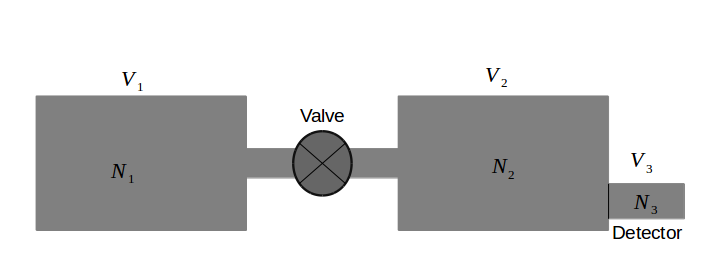
\includegraphics[width=0.9\textwidth]{volume_schematic.png}
  \caption[Schematic drawing of a simple UCN source]{Schematic drawing
    of a simple UCN source. $V_1$ is the production volume with $N_1$
    number of UCN, $V_2$ is the secondary volume where $N_2$ number of
    UCN exist, and $V_3$ is the detector with $N_3$ number of UCN. }
  \label{fig:volume_schematic}
\end{figure}

At $t = 0$, when the beam is on and the valve is closed, the number of UCN in
$V_1$ builds up, while the total number of UCN in $V_2$ and $V_3$ is
zero. This may be described with 

\begin{equation}
  \label{eqn:dndt}
\frac{dN_1}{dt} = P - \frac{N_1}{\tau_1}~,
\end{equation}
where $P$ is the UCN production rate in the source, as described in
Section~\ref{sec:UCN_production}, and $\tau_1$ is the UCN storage
lifetime in the source. The solution is exponential
$N_1 \rightarrow P \tau_1$ as $t \rightarrow \infty$. After the beam
is turned off, the valve is opened, and UCN may travel to the volume
$V_2$ and eventually volume $V_3$. In our measurements, the valve is
usually left open for 2 minutes. The UCN rates of change are described
by the coupled, first-order, linear differential equations:
%trade between $V_1$, $V_2$
%and $V_3$ is described by the differential Eqn.~\ref{eqn:alldndt}.

\begin{equation}
  \label{eqn:alldndt}
  \begin{aligned}
    \frac{dN_1}{dt} =&- \frac{N_1}{\tau_{c,1}} - \frac{N_1}{\tau_1} + \frac{N_2}{\tau_{c,2}}  \\
    \frac{dN_2}{dt} =& \frac{N_1}{\tau_{c,1}} - \frac{N_2}{\tau_{c,2}} - \frac{N_2}{\tau_2} - \frac{N_2}{\tau_{c,3}} \\
    \frac{dN_3}{dt} =& \frac{N_2}{\tau_{c,3}}~.
  \end{aligned}
\end{equation}

Here $\tau_{c,1}$, $\tau_{c,2}$, and $\tau_{c,3}$ are the lifetimes
due to crossing the surface and $\tau_2$ is the lifetime in $V_2$. In
these equations, $dN_1/dt$ shows the change in the UCN counts over
time in $V_1$, $dN_2/dt$ shows the change in the UCN counts in $V_2$,
and $dN_3/dt$ shows the change in the UCN count in $V_3$, after the
valve is opened. Each term in the right side of the equations is
described below.

In the first equation, the total number of UCN in $V_1$ depends on
three factors: the UCN that get into $V_2$ with the rate
$N_1/\tau_{c,1}$, the UCN that is lost with the storage lifetime
$\tau_1$ with the rate rate $N_1/\tau_{1}$, and the UCN that bounce
back from $V_2$ to $V_1$ with the rate $N_2/\tau_{c,2}$. Here
$1/\tau_{c,1}$ is the probability of UCN crossing from volume $V_1$ to
volume $V_2$, and $1/\tau_{c,2}$ is the probability of UCN cross from
volume $V_2$ back to volume $V_1$.


In the second equation for $V_2$, some UCN cross from $V_1$ to $V_2$
with the rate $N_1/\tau_{c,1}$, some get lost with the rate
$N_2/\tau_2$, some cross the gate valve and go back to $V_1$ with the
rate$N_2/\tau_{c,2}$, and some get to the detector with the rate
$N_2/\tau_{c,3}$. Here $1/\tau_{c,3}$ is the probabiliy of UCN
crossing from volume $V_2$ to volume $V_3$ and $1/\tau_2$ is the loss
probability of UCN in volume $V_2$.



In the third equation, the rate of the UCN detection $dN_3/dt$ is the
rate of UCN crossing from volume $V_2$ to volume $V_3$ as
$N_2/\tau_{c,3}$. If they enter $V_3$, they will be detected, hence,
they will not cross back.  In principle, solving these equations could
give an estimate of the number of UCN in each volume. The solutions
are again exponentials.

A 3D drawing of the experimental setup is shown in
Fig.~\ref{fig:Source_all}. In this case, $V_1$ is the UCN source
bottle and the horizontal section of the UCN guide before the UCN gate
valve, and $V_2$ and $V_3$ are the volumes after the UCN valve and the
detector volume respectively.


The process of UCN production described above is refered to as ``batch
mode'', since the UCN are accumulated in the source before opening the
UCN valve.
%Here the target is irradiated, and the UCN are produced in
%the source. After the irradiation stops, the UCN valve is opened, and
%UCN could bounce of the guide walls and reach the detector volume.
In our standard UCN production measurements, the applied beam current
is 1~$\mu$A, and the target is irradiated for 60~s. One cycle of
measurement is shown in Fig.~\ref{fig:UCNRate}. The UCN valve is
typically left open for 2 minutes. The end of a UCN cycle is defined
by the UCN valve close time. Once the UCN valve is closed, a new cycle
of measurement starts. The UCN counts are then fitted by an
exponential function.


\begin{figure}[h!]
  \centering
  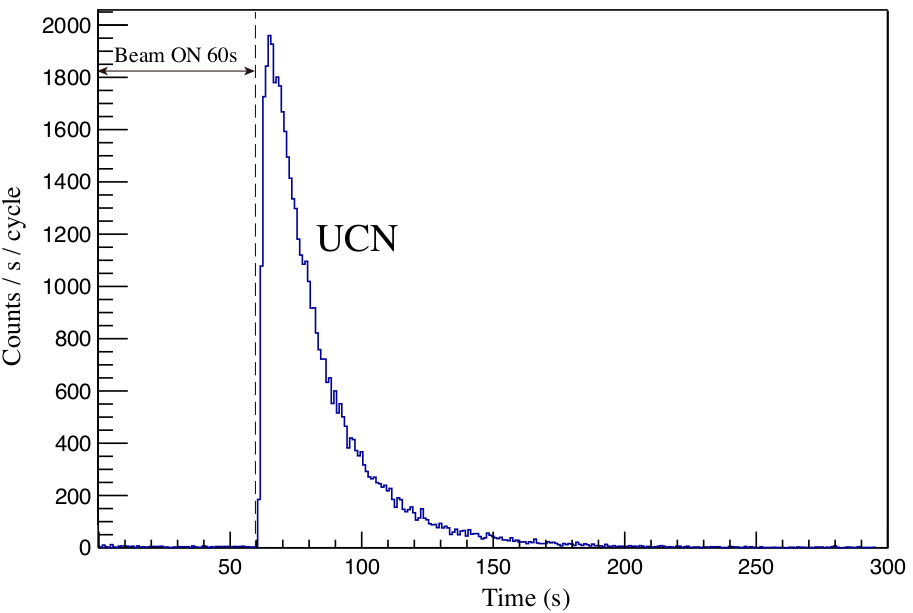
\includegraphics[width=0.8\textwidth]{UCNRate.png}
  \caption[UCN rate at 1~$\mu$A beam current and 60~s target
  irradiation]{The figure shows the UCN rate at 60~s irradiation time,
    and 1~$\mu$A beam current. In this case, the UCN gate valve is
    opened immediately after the end of target irradiation. At this
    time, the UCN rate reaches the peak of about 2000 UCN/s. The UCN
    rate decays down to the background level. The valve is left open
    for 120~s. }
  \label{fig:UCNRate}
\end{figure}


Another possible mode of operation is to leave the UCN valve open
while irradiating the target. This is called the ``steady-state mode''
where we have a constant stream of UCN to the main detector~(see
Section~\ref{sec:steadystate}).

The following sections are focused on the result of the UCN yield
optimization, the UCN storage lifetime measurements, UCN production in
the steady-state mode and the comparison of those measurements with
simulations.


\section {Data Quality Checks}
During the 2017 experimental run, we performed about 35 experiments
individually labelled by TCN\#. For most of these experiments we used
the $^6\mathrm{Li}$ detector described in
Section~\ref{sec:Li6detector}. The data in this chapter was focused on
UCN source characterization, all acquired with the $^6\mathrm{Li}$
detector.  To check the reliability of this data we performed data
quality checks based on the detector signals.

%The main detector for most of the experiments is the $^6\mathrm{Li}$
%glass based scintillator detector described in
%Section~\ref{sec:Li6detector}. Before using the collected data to
%extract the desired information, it is critical to make sure that the
%detector was working as expected, and that the data is reliable. Here
%some data quality checks are reported.


The PSD versus $Q_L$ distribution from a run is shown in
Fig.~\ref{fig:psd_vs_ql} for all nine PMTs combined. The UCN appear in
the upper right portion of PSD-$Q_L$ space.
% The graph is for run 541
\begin{figure}[h!]
  \centering
  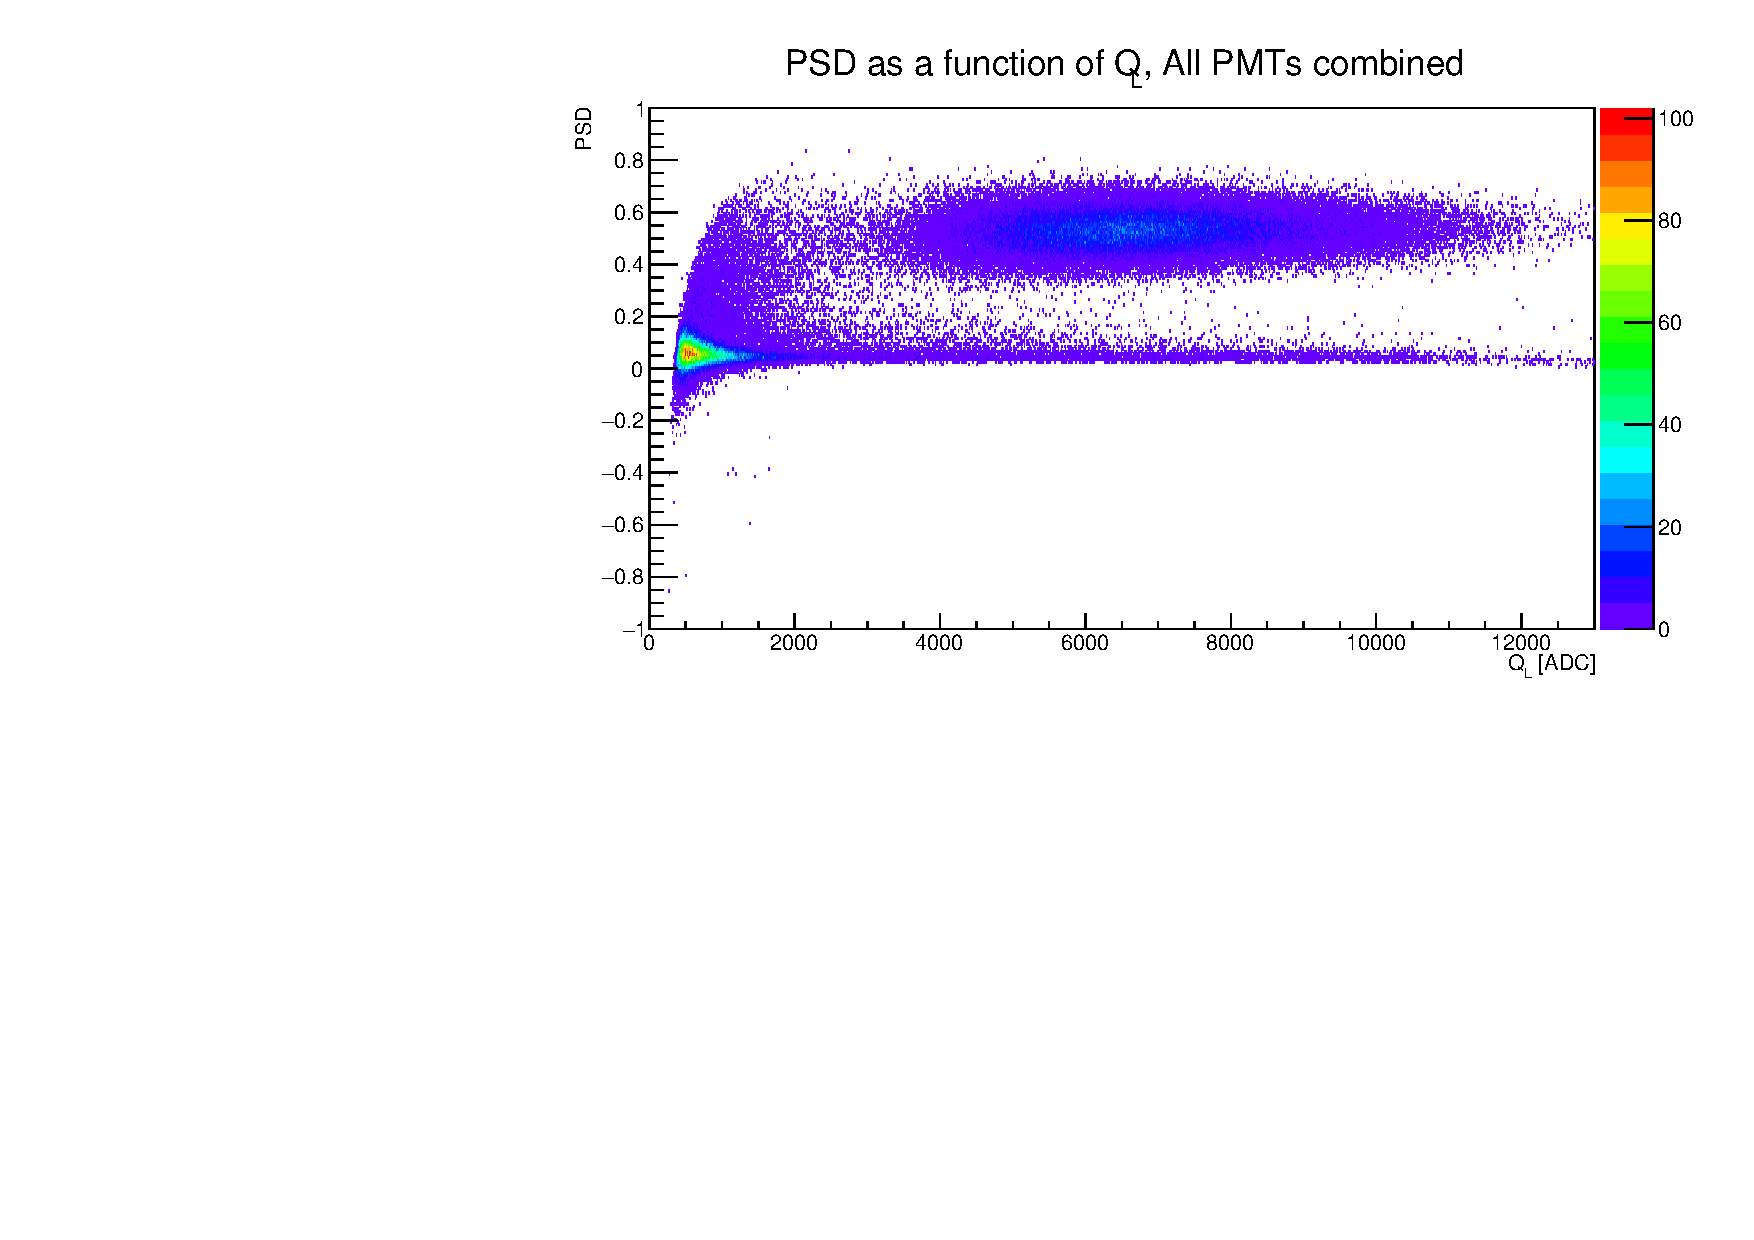
\includegraphics[width=0.9\textwidth]{PSD_vs_QL.pdf}
  \caption[UCN event spectra for 1~$\mu$A beam current and 60~s target
  irradiation]{UCN event spectra for all of the PMTs for a standard
    1~$\mu$A proton beam current and 60~s target irradiation time }
  \label{fig:psd_vs_ql}
\end{figure}

Here the UCN spectrum has an energy range of 3000 to 12000 $Q_L$ as
expected, and a median PSD value of 0.5. The events at PSD~$\sim 0$
represent the $\gamma$-rays in the lightguides. To define UCN counts,
a PSD cut at 0.3 and a $Q_L$ cut at 2000 were applied. Those cuts were
confirmed with Monte-Carlo simulations to have an efficiency of 99\%
or higher. The total number of UCN events in each PMT for a run at
1~$\mu$A beam current and 60~s irradiation time is shown in
Fig.~\ref{fig:channelcounts}.  Out of all 9 channels, the central
channel counts the most UCN, while the corner channels receive the
least as expected based on geometry.
% for run 573
\begin{figure}[h!]
  \centering \includegraphics[width=0.9\textwidth]{PMTROIevents.pdf}
  \caption[UCN events per channel]{Number of UCN events for each
    channel. The total number of UCN events decrease as we move
    towards the corner channels.  }
  \label{fig:channelcounts}
\end{figure}


The effect of detector systematics on the measured UCN counts can be
categorized in three groups: deadtime, crosstalk and pileup. Deadtime
is the minimum time difference between two subsequent UCN events in
the same PMT, which gives rise to a loss of UCN counts. Crosstalk
arises from multiple trigger events in neighboring PMTs originated
from the same UCN event. This would falsely increase the total UCN
counts. Pileup is the combination of multiple events into a single
event. It includes UCN-UCN, UCN-$\gamma$, $\gamma$-UCN and
$\gamma$-$\gamma$ pileups. The true number of UCN counts is estimated
by
\begin{equation}
  \label{eqn:trueUCN}
  N^{\mathrm{True}}_{\mathrm{UCN}} = \left [ N^{\mathrm{raw}}_{\mathrm{UCN}} \cdot \left( 1 + \alpha_{pl} + \alpha_{ct}\right) \right] \cdot A_{box}~,
\end{equation}
where $\alpha_{pl}$ is the estimated pileup coefficient from data and
independant calculations assuming Poisson statistics, $\alpha_{ct}$ is
the estimated time-coincidence analysis on data, and $A_{box}$ is the
UCN box efficiency estimated using Monte-Carlo simulations. Based on
our Monte-Carlo simulations, the $\gamma$-UCN and UCN-$\gamma$ pileups
are not a concern for UCN counting. In addition, $\gamma$-$\gamma$
pileup does not leak into the UCN box.

The result of such analyses showed the UCN box acceptance is at 99.7
$\pm$ 0.1~\%. The UCN-UCN pileup at 1~$\mu$A beam current and 60~s
irradiation of the target was measured to be at 0.075~Hz or has and
effect of less than 1\%. The analysis indicated that cross-talk has a
negligible effect on the operating rates and deadtime affects the
rates by less than 2\%.


%% I should think about adding MC simulations by Pietro, maybe???
%%

\section{UCN Count Measurements \label{UCNCounts}}

The total number of produced UCN in the vertical source, $N$, at a
certain time t$_i$, when the UCN valve is closed is the integration of
Eqn.~\ref{eqn:dndt}
\begin{equation}
  \label{eq:totalUCN}
  N = P \tau_1\left[ 1- \exp \left(\frac{-t_i }{ \tau_1}\right) \right]~,
\end{equation}
where the UCN storage lifetime $\tau_1$ is given by

\begin{equation}
  \label{eqn:tau1}
  \frac{1}{\tau_1} = \frac{ f_1}{\tau_\mathrm{He}} + \frac{1-f_1}{\tau_\mathrm{vapour}}+\frac{1}{\tau_\mathrm{wall,1}} + \frac{1}{\tau_\beta}~.
\end{equation}
The storage lifetime consists of four terms: the loss rate in the
superfluid helium $ f_1\tau_\mathrm{He}^{-1}$, the loss rate in the
helium vapour $(1-f_1)\tau_\mathrm{vapour}^{-1}$, the loss rate in the
UCN guide walls $\tau_\mathrm{wall,1}^{-1}$, and the neutron $\beta$
decay $\tau_\beta^{-1}$. The volume in which the UCN are produced
includes the UCN bottle, as well as the horizontal guide section
before the UCN valve~(see Fig.~\ref{fig:Source_all}). This volume is
not fully filled with the superfluid helium. The quantity $ f_1$ is
the probablity of UCN being in the superfluid helium while the UCN
valve is closed. After the valve is opened, the total UCN lifetime is

\begin{equation}
  \label{eqn:tau2}
  \frac{1}{\tau_2} = \frac{ f_2}{\tau_\mathrm{He}} + \frac{1-f_2}{\tau_\mathrm{vapour}}+ \frac{1}{\tau_\mathrm{wall,2}}+\frac{1}{\tau_d} + \frac{1}{\tau_\beta}~,
\end{equation}
where $f_2$ is the probability of UCN being in the superfluid helium,
${\tau_\mathrm{wall,2}}^{-1}$ is the UCN guide loss rate in the case
where the valve is open and the target irradiation is stopped, and
$\tau_d^{-1}$ is the loss rate in the
detector. Fig.~\ref{fig:UCNRate_with_lines} shows three measurement
cycles at 1~$\mu$A beam current, and 60~s irradiation time with zero
second delay time between the end of the target irradiation and
opening the UCN valve~(here sometimes this is referred to as the cycle
delay time or valve open delay time). The dashed lines indicate the
start of the target irradiation for a cycle, the dotted lines show the
end of the target irradiation, which in this case is the same as the
UCN valve open time. The solid lines shows the valve close time.


\begin{figure}[h!]
  \centering
  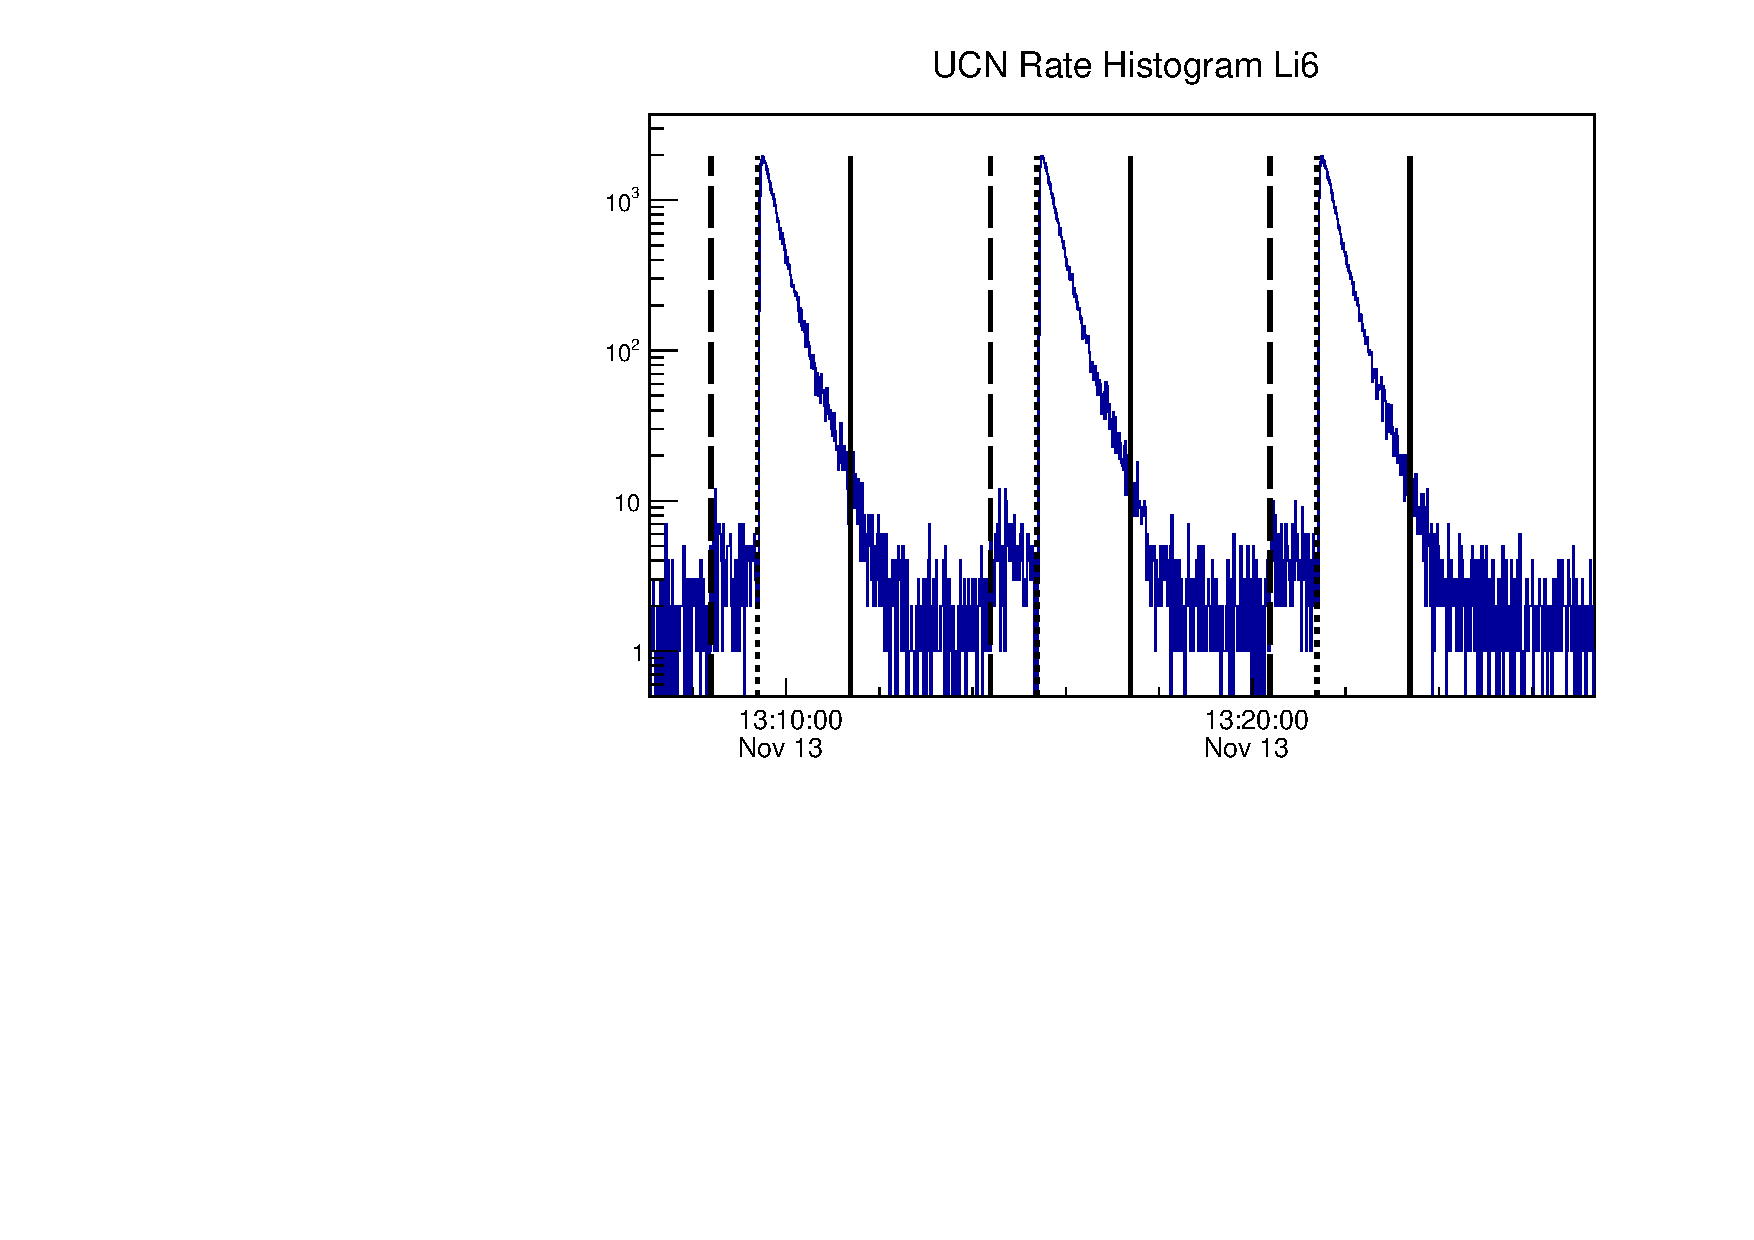
\includegraphics[width=1.0\textwidth]{UCNRate_with_lines_logy.pdf}
  \caption[UCN cycles of measurement]{Three measurement cycles for
    1~$\mu$A beam current, 60~s irradiation time, and 0~s valve open
    delay time. The dashed lines show the start of the target
    irradiation, the dotted lines show the end of the irradiation and
    the valve open time for each cycle and the solid lines show the
    end of a cycle, which is the valve close time.}
  \label{fig:UCNRate_with_lines}
\end{figure}

The total UCN counts are given by the sum of all the UCN events for
the duration of the valve open time. However, this method of counting
includes backgrounds. To subtract the background counts from the
actual UCN counts, the UCN background rate is calculated before the
start of the irradiation of that particular cycle. This rate is then
multiplied by the valve open duration, which then gives an estimate of
the total background UCN counts. The background rate is typically less
than 5~UCN/s. The subtraction of the latter from the total UCN counts
gives the actual number of UCN that are produced by the isopure helium
converter, and detected by the detector. At low and moderate UCN
counts, the statistical uncertainty is available by taking the square
root of the number of measured events, as follows conveniently from
Poisson statistics~\cite{pomme2015uncertainty}.
%%%%%%%%%%
\subsection{UCN Yield Versus Proton Beam Current}

A unique feature of the TRIUMF facility compared to RCNP is higher
current compatibility~(RCNP: 400~MeV at $<1$~$\mu$A).
Fig.~\ref{fig:counts_vs_beam} shows the total UCN counts versus the
applied proton beam current in $\mu$A at 60~s irradiation time. The
background UCN is subtracted off from the detected UCN counts as
explained earlier. The statisticl uncertainty on the UCN counts is
calculated as $\sqrt{N}$. At lower beam currents, the total UCN counts
increase linearly with the proton beam current. The dashed line shows
the extrapolation to higher beam currents in an ideal case. However,
at higher beam currents, the total UCN counts deacreses due to an
increase in the heat load on the isopure superfluid helium, and
therefore, its temperature. Theoretically, the upscattering rate in
the superfluid helium is related to its temperature as $T^7$~(see
Section~\ref{sec:upscattering}). This has been confirmed by performing
PENTrack simulations and comparing the result to the acquired
data~(see Section~\ref{sec:pentrack}).



\begin{figure}[h!]
  \centering
  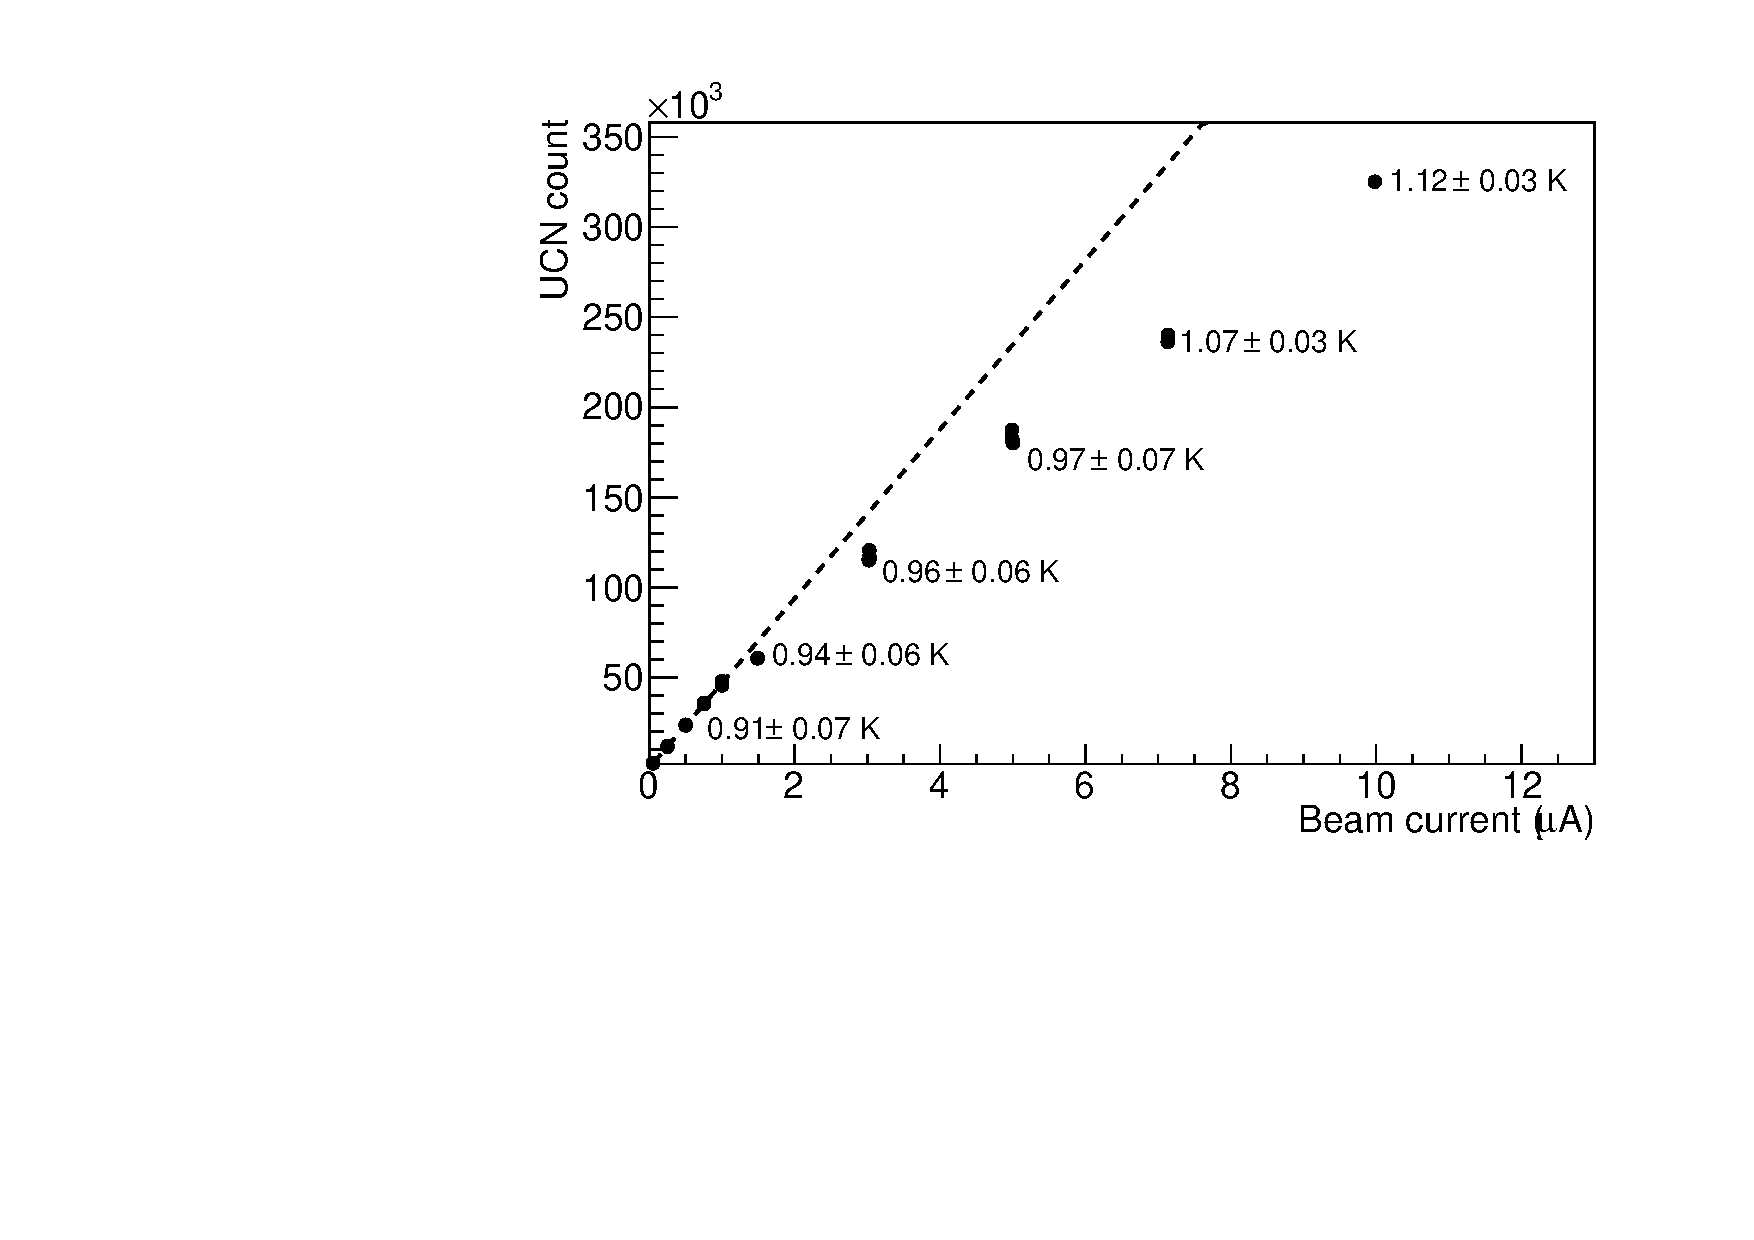
\includegraphics[width=0.8\textwidth]{UCNCounts_vs_Beam.pdf}
  \caption[UCN counts versus proton beam current]{The total UCN counts
    versus the applied proton beam current for 60~s target irradiation
    times. The labels show the full range of the superfluid helium
    temperature for that measurement. The dashed line is the fit to
    the UCN counts at low beam currents. The total UCN counts can be
    described by Eqn.~\ref{eq:totalUCN}. Here the production rate
    grows linearly with current and $\tau_1$ varies with time.}
  \label{fig:counts_vs_beam}
\end{figure}


The labels in the graph show the full range of the isopure helium
temperatures during the measurement cycle. Four temperature sensors
were used to measure the superfluid helium temperature with the
following names in our EPICS system: TS11, TS12, TS14 and TS16. The
location of these sensors are shown in Fig.~\ref{fig:TSs}. The
temperature sensor TS11 is located at the UCN heat exchanger bottom,
the temperature sensor TS14 is located at the UCN heat exchanger top,
the temperature sensor TS12 is located at the UCN double tube bottom,
and the temperature sensor TS16 is located at the UCN double tube
top. At low temperatures around 0.8~K, these temperature sensors show
a maximum of 0.1~K discrepancy with TS16 showing the highest value,
and TS12 showing the lowest value.


\begin{figure}[h!]
  \centering
  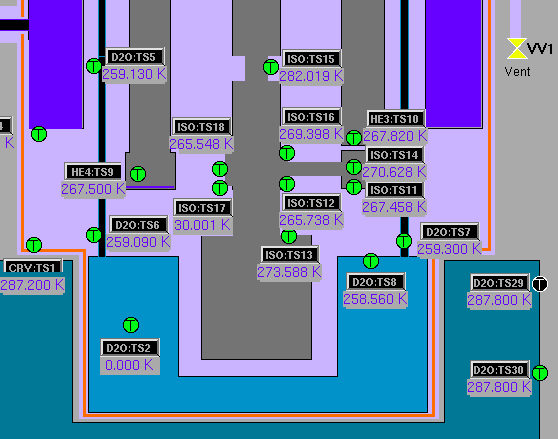
\includegraphics[width=0.8\textwidth]{TSs.png}
  \caption[TUCAN's EPICS temperature monitoring screen~(zoomed
  in)]{Zoomed in screenshot of the EPICS temperature monitoring
    screen~\ref{fig:epics}. TS11 is located at the UCN heat exchanger
    bottom, TS12 is located at the UCN double tube bottom, TS14 is
    located at the heat exchanger double tube top and TS16 is located
    at the UCN double tube top. For further information about the
    source schematic see Section~\ref{sec:vertical_source}}
  \label{fig:TSs}
\end{figure}

At lower beam currents, because of the low heat load on the superfliud
helium, its temperature change is not significant, and it gives rise
to a linear increase in the UCN counts versus at various applied
proton beam current. However, at higher proton beam currents, the
temperature of the superfluid increases due to a higher heat load, and
it gives rise to higher upscattering rate in the superfluid and lower
UCN counts.


\subsection{UCN Yield Versus Target Irradiation Times}
The total UCN counts are optimized by irradiating the target with
different proton beam currents for different irradiation times. The
result is shown in Fig.~\ref{fig:counts_vs_irrad}. In this graph, the
vertical axis shows the total number of UCN counts where the
background UCN are subtracted, and the horizontal axis shows the
target irradiation times in seconds. Each marker represents a proton
beam current. The dashed line is an exponential fit~(see
Eqn.~\ref{eq:totalUCN}) to those data points. The proton beam current
and the extracted time constant from the fit are shown in the Figure.

At higher beam currents, the saturation time constant decreases due to
the higher heat load and faster temperature increase in the superfluid
helium. At higher beam currents and longer irradiation times, the
total measured UCN counts are below the exponential extrapolation due
to the higher temperature and higher upscattering rate in the
superfluid helium.

\begin{figure}[h!]
  \centering
  \includegraphics[width=0.8\textwidth]{UCNCounts_vs_irradTime.pdf}
  \caption[UCN yield versus target irradiation times]{Number of UCN
    extracted from the source after irradiating the target for
    different times with different beam currents. The dashed lines
    extrapolate the data for irradiation times below 60~s using
    exponential saturation curves. The labels show the saturation time
    constant for each beam current. }
  \label{fig:counts_vs_irrad}
\end{figure}


\subsection{UCN Yield Versus Isopure Helium Temperature}
The UCN counts were also measured at different superfluid helium
temperature~(see Fig.~\ref{fig:counts_vs_temp}). The vertical axis
shows the number of UCN counts, and the horizontal axis shows the
temperature of the superfluid helium for all four temperature
sensors. The vertical error bars are $\sqrt{N}$, and the horizontal
error bars are calculated as $(T_{\mathrm{max}}-T_{\mathrm{min}})/2$
for each temperature sensor, where $T_{\mathrm{max}}$ is the maximum
value of the superfluid helium temperature reading by one temperature
sensor, and $T_{\mathrm{min}}$ is the minimum value read for the same
sensor.

\begin{figure}[h!]
  \centering
  \includegraphics[width=0.9\textwidth]{counts_vs_temp.pdf}
  \caption[UCN yield versus the superfluid helium temperature]{UCN
    yield versus the superfluid helium temperature. At a particular
    UCN counts, there are several values for the temperature of the
    superfluid helium. This is due to the discrepancy in the
    temperature sensor readings as described in the text.}
  \label{fig:counts_vs_temp}
\end{figure}

As the temperature of the superfluid helium increases, the number of
UCN counts in the detector decreases as expected. This is mainly due
to the high UCN upscattering rate in the superfluid helium at higher
temperatures which is further quantified in
Section~\ref{sec:yieldsims}.


\subsection{Steady-state UCN Production\label{sec:steadystate}}

The result shown so far are achieved in the batch mode of
operation. In addition to such measurements, the UCN rate was also
measured at different beam currents in the steady-state mode of
operation. In these measurements, the UCN valve was left open, and the
target was irradiated for about 10~min. A typical UCN rate graph for
0.3~$\mu$A beam current and 10~min target irradiation time is shown in
Fig.~\ref{fig:UCNRate_steadystate}.


\begin{figure}[h!]
  \centering
  \includegraphics[width=0.9\textwidth]{steadystate_point3muA.png}
  \caption[Steady-state UCN rate at 0.3~$\mu$A beam current]{UCN rate at the
    steady-state production mode with 0.3~$\mu$A proton beam
    current. The UCN rate reaches a constant value of 450 UCN
    counts/s.}
  \label{fig:UCNRate_steadystate}
\end{figure}

At lower beam currents such as 0.3~$\mu$A, the UCN rate remains
constant throughout the whole target irradiation time as shown in
Fig.~\ref{fig:UCNRate_steadystate}. An example of a steady-state UCN
production at 3~$\mu$A is shown in
Fig.~\ref{fig:UCNRate_steadystate_highbeam}. Since the proton beam
current is high, the UCN rate does not remain constant. Here the
maximum UCN rate is observed near the start of the target
irradiation. As the target irradiation continues, the heat load on the
cryostat increases the temperature, and the upscattering rate in the
superfluid helium. As a result, the UCN rate decreases. The change in
the temperature is shown in Fig.~\ref{fig:UCNRate_temp}. Throughout
the target irradiation time, the temperature of the superfluid helium
increases. Once the irradiation stops, the temperature starts to
decrease.


\begin{figure}[h!]
  \centering
  \includegraphics[width=0.9\textwidth]{654_UCNRate.pdf}
  \caption[Steady-state UCN rate at 3~$\mu$A beam current]{The UCN
    rate at 3~$\mu$A beam current at 10~min irradiation time at the
    steady-state mode of operation. The UCN valve is left open
    throughout the measurement cycle. Quickly after the start of the
    target irradiation the UCN rate in the detector goes up. The
    target irradiation creates a heatload on the cryostat and the
    superfluid helium. This gives rise to a slow temperature increase
    in the source. As a result, the UCN rate goes down due to the
    higher upscattering rate.  }
  \label{fig:UCNRate_steadystate_highbeam}
\end{figure}

\begin{figure}[h!]
  \centering
  \includegraphics[width=0.9\textwidth]{UCNRate_temp.pdf}
  \caption[Superfluid helium temperature at 3~$\mu$A beam
  current~(steady-state mode)]{The temperature of the superfluid
    helium~(TS12) for the steady state mode of operation at 3~$\mu$A
    beam current and 10~min target irradiation. After the irradiation
    stops, the temperature starts to decrease. }
  \label{fig:UCNRate_temp}
\end{figure}


The steady-state UCN rate measurements were conducted at different
proton beam currents, leading to different temperature changes for all
temperature sensors. The result of all those measurements and
comparison to simulations are discussed in Section~\ref{sec:pentrack}.


%are shown in
%Fig.~\ref{fig:rate_vs_temp}. Here the vertical axis is the measured
%UCN rate normalized to the proton beam current and the horizontal axis
%is the temperature of the superfluid helium for all temperature
%sensors.


%\begin{figure}[h!]
%  \centering
%  \includegraphics[width=0.7\textwidth]{rate_vs_temp.pdf}
%  \caption{Histogram of measured UCN rates and temperatures from all
%    four temperature sensors while the target is continuously
%    irradiated with the UCN valve open. The four solid lines are fits
%    of equation~\ref{eq:steadystaterate} to the data for each individual temperature
%    sensor.}
%  \label{fig:rate_vs_temp}
%\end{figure}


%The rate of the detected UCN is given by

%\begin{equation}
%  \label{eqn:rate}
%  R = \frac{P \tau_3}{\tau_d} = \frac{P \tau_d^{-1}}{\tau_\mathrm{wall,2}^{-1} + \tau_d^{-1} + f_\mathrm{He,3}\tau_\mathrm{He}^{-1}}
%\end{equation}
%where $\tau_d^{-1}$ is the loss rate in the detector,
%${\tau_\mathrm{wall,2}}^{-1}$ is the UCN guide wall loss and
%$\tau_\mathrm{He}^{-1}$ is the loss rate in the superfluid helium.
%Assuming $\tau_\mathrm{He}^{-1} = B \left( T \right)^a$ the
%Eqn.~\ref{eqn:rate} could be written as

%\begin{equation}
%R(T) = \frac{c}{1 + b \left( \frac{T}{\SI{1}{\kelvin}} \right)^{a}}
%\label{eq:steadystaterate}
%\end{equation}
%where \large
%$b = \frac{f_{\mathrm{He,3}}B}{\tau^{-1}_{\mathrm{wall,2}}
%  +\tau^{-1}_d}$ \normalsize and \large
%$c = \frac{P\tau^{-1}_d}{\tau^{-1}_{\mathrm{wall,2}} +\tau^{-1}_d}$
%\normalsize.  Eqn.~\ref{eq:steadystaterate} can be used to fit the
%data shown in Fig.~\ref{fig:rate_vs_temp}.  Since the four temperature
%sensors in the superfluid helium deviate by up to \SI{0.1}{\kelvin},
%the rate for each temperature sensor is fitted individually (see
%table~\ref{tab:steadystateparams}). The exponent $a$ can be directly
%determined this way, giving
%\begin{equation}
%a = 7.02 \pm 0.02_\mathrm{stat.} \pm 0.53_\mathrm{syst.},
%\label{eq:a}
%\end{equation}
%which is in good agreement with the theoretical prediction of $a = 7$
%(see Sec.\ref{sec:upscattering}). Here the statistical error comes
%from the fit and the systematic error comes from the temperature
%difference from the sensors and their propagated error.


%The other parameters are
%\begin{align}
%\label{eq:b}
%  b =&  0.0995 \pm 0.0007_\mathrm{stat.} \pm 0.0298_\mathrm{syst.} \\
%  c =& (1610 \pm 1_\mathrm{stat.} \pm 75_\mathrm{syst.}) \, \si{\per\second}
%\end{align}

%\begin{table}[h!]
%  \centering
%  \begin{tabular}{|c|c|c|c|}
%    \hline
%      Temp. sensor & $a$ & $b$ & $c$ (\si{\per\second}) \\
%      \hline
%      TS11 & $7.55 \pm 0.03$ & $0.0697 \pm 0.0009$ & $1535 \pm 1$ \\
%      \hline
%      TS12 & $6.48 \pm 0.03$ & $0.1293 \pm 0.0016$ & $1606 \pm 2$ \\
%      \hline
%      TS14 & $7.34 \pm 0.03$ & $0.0832 \pm 0.0011$ & $1555 \pm 2$ \\
%      \hline
%      TS16 & $6.67 \pm 0.04$ & $0.1215 \pm 0.0019$ & $1685 \pm 3$ \\
%      \hline
%    \end{tabular}
%  \caption{Parameters determined by fitting equation
%    \ref{eq:steadystaterate} to the measured rates shown in
%    fig. \ref{fig:rate_vs_temp} for each individual temperature
%    sensor.}
%  \label{tab:steadystateparams}
%\end{table}

\subsection{UCN Yield Over the Experiment Period}

The total UCN counts for our standard measurements at 1~$\mu$A beam
current and 60~s irradiation time over the course of the experimental
run is shown in Fig.~\ref{fig:UCNCounts_time}. The graph shows an
overall decrease of about $\sim$~40\% over the course of the eighteen
days. The source volume is connected to a long UCN guide sealed with
an O-ring. It is expected that the rest gas added contaminants to the
source every time the UCN valve is opened. This caused a decrease in
the UCN yield~(and storage lifetime as shown later in
Section~\ref{sec:storage_overall}) over the course of the
measurement. In addition, the changes in the UCN guide geometry in the
latter half of the run potentially affected this drop.


\begin{figure}[h]
  \centering
  \includegraphics[width=0.9\textwidth]{UCNCounts_vs_time.pdf}
  \caption[ UCN yield at 1~$\mu$A beam current and 60~s target
  irradiation over experimental run]{The total UCN counts extracted
    from the source for 1~$\mu$A beam current and 60~s irradiation
    time at different days during the experimental run. }
  \label{fig:UCNCounts_time}
\end{figure}

\section{UCN Storage Lifetime~\label{storagelifetime}}

The total number of detected UCN strongly depends on the storage
lifetime of the source $\tau_1$~(see Eqn.~\ref{eqn:tau1}) which
indicates the performance of the UCN source. The storage lifetime of
UCN is determined by measuring the detected UCN at different valve
open delay times right after the irradiation stops.  The typical
chosen values are 0~s, 5~s, 10~s, 20~s, 30~s, 60~s, 80~s, 120~s and
170~s. The target was irradiated for 60~s.
% For most of the experiments, the order in which the delay to the
% valve open time was applied was as following: 0~s, 170~s, 20~s,
% 120~s, 50~s, 80~s, 30~s and 5~s.
The exponential decay constant in the fit to the total UCN counts
without the background, for different valve open delay times, is the
total storage lifetime in the source.

Fig.~\ref{fig:storage_all} shows several UCN cycles for the standard
1~$\mu$A proton beam current and 60~s target irradiation time. The
difference in the maximum detected UCN rate is due to different valve
open delay times as labeled on the graph.
% used to be storagetime_all.png
\begin{figure}[h!]
  \centering
  \includegraphics[width=1.0\textwidth]{UCNrate_withdelaylabels.pdf}
  \caption[UCN rate at different value open delay times at 1~$\mu$A
  beam current and 60~s irradiation time ]{UCN cycles at different
    valve open delay times for 1~$\mu$A beam current and 60~s target
    irradiation time. The vertical dashed line indicate the start of
    the target irradiation. The values in seconds represent the valve
    open delay times for each cycle.}
  \label{fig:storage_all}
\end{figure}
Fig.~\ref{fig:storage_example} shows the total UCN counts~(background
subtracted) versus the valve open delay time for 1~$\mu$A and
10~$\mu$A proton beam current and 60~s target irradiation time. The
total UCN counts at 0~s cycle delay time are higher for 10~$\mu$A. The
longer delay times give rise to lower UCN counts due to the loss
mechanisms. The one exponential fit function
\begin{equation}
\text{UCN counts} = A e^{-t/\tau_1}~,
\end{equation}
determines the storage lifetime $\tau_1$. At 170~s valve open delay
time, the total UCN counts are not consistent with what the fit
function predicts due to low statistics. However, the result of the
fit is not driven by this inconsistency as it has a negligible effect
on the extracted storage lifetime because of low statistics.
%\begin{figure}[h!]
%  \centering
%  \includegraphics[width=0.9\textwidth]{17002_StorageLifetime.pdf}
%  \caption{The total UCN counts at different valve open delay times
%    for 1~$\mu$A beam current and 60~s irradiation time. The red line
%    is the one exponential fit. }
%  \label{fig:storage_example}
%\end{figure}

%\setlength\belowcaptionskip{-3ex}
\begin{figure}[h!]
  \centering
  \begin{subfigure}{.8\textwidth}
    \centering
    \includegraphics[width=1.0\textwidth]{17002_StorageLifetime_ver3.pdf}
    \caption{}
    \label{fig:storage_example1}
  \end{subfigure}%
  \\
  \begin{subfigure}{.8\textwidth}
    \centering
    \includegraphics[width=1.0\textwidth]{10muA_30s_ver3.pdf}
    \caption{}
    \label{fig:storage_example10}
  \end{subfigure}
  \caption[UCN storage lifetime extraction for two beam currents]{The
    total UCN counts at different valve open delay times for (a)
    1~$\mu$A beam current and 60~s irradiation time and (b) 10~$\mu$A
    beam current and 30~s target irradiation time. The red line is the
    one exponential fit. The initial UCN counts for the 10~$\mu$A
    target irradiation is higher. However, the storage lifetime is
    lower compared to 1~$\mu$A beam current because of the heat load
    on the superfluid helium. In the case of 10~$\mu$A beam current,
    the maximum cycle delay time is 120~s compared to the 170~s delay
    time in the case of 1~$\mu$A beam current. This is due to
    excessive heat load on the cryostat and low statistics.}
  \label{fig:storage_example}
\end{figure}

% Below the result of the storage lifetime measurements are presented.

\subsection{Storage Lifetime Versus Beam Current and Irradiation Time}
The storage lifetime of UCN in the source is measured at different
proton beam currents and different target irradiation times for a
better understanding of the source. The result of those measurements
is shown in Fig.~\ref{fig:storage_beam_irrad}. Here the vertical axis
shows the storage lifetime in the source in seconds, and the
horizontal axis shows the proton beam current in $\mu$A. Each marker
represents a target irradiation time. At lower beam currents, the
duration of the target irradiation does not make a significant
difference in the storage lifetime. At higher proton beam currents,
the longer the irradiation time takes, the lower the storage lifeimte
will be. In summary, irradiating the target at high proton beam
currents and longer irradiation times create a higher heat load on the
UCN source, which leads to higher upscattering rates, and as a result,
lower UCN storage lifetime in the source.

\begin{figure}[h!]
  \centering
  \includegraphics[width=0.9\textwidth]{StorageLifetime_17009_and_17009A.pdf}
  \caption[UCN storage lifetime at different irradiation times and
  proton beam currents]{Storage lifetime in the source at different
    irradiation times and proton beam currents. Different markers
    refer to different target irradiation times. At longer irradiation
    times and higher beam currents, the storage lifetime decreases due
    to the increased heat load in the source, and an increase in the
    superfluid helium temperature.}
  \label{fig:storage_beam_irrad}
\end{figure}


\subsection{Storage Lifetime Versus Isopure Helium Temperature}
The storage lifetime of UCN was also measured at different
temperatures of the superfluid helium. In this experiment, the
temperature of superfluid was increased by using heater wire wrapped
around the UCN bottle. The heater powers were set to increase the
temperatures by a certain amount. Once the temperatures stablized,
target irradiation was started.

The result of this measurement is shown in
Fig.~\ref{fig:storagelifetime_vs_temp}. The vertical axis is the
storage lifetime of UCN in seconds, and the horizontal axis is the
temperature of the superfluid helium. As mentioned earlier, the four
temperature sensors that measure the temperature of the superfluid
show some discrepancy. As a result, for a given measurement, there are
four different values for the temperature of the superfluid. The
vertical error bars come from the fit, and the horizontal error bars
are set as ($T_{\mathrm{max}} - T_{\mathrm{min}}$)/2, as discussed
earlier. The data shows a downward trend. As the temperature of the
superfluid helium increases, the storage lifetime in the source
decreases. This is due to higher upscattering rate in the superfluid
helium at higher temperatures.


%TCN17014
\begin{figure}[h!]
  \centering
  \includegraphics[width=0.9\textwidth]{StorageLifetime_vs_temp.pdf}
  \caption[UCN storage lifetime at different isopure helium
  temperatures]{Storage lifetime of UCN at different isopure helium
    temperatures. In this experiment, the temperature of the
    superfluid helium was set using heater tapes around the UCN
    bottle. The vertical axis shows the storage lifetime in seconds
    and the horizontal axis shows the superfluid helium temperature in
    Kelvin. As the temperature increases, the storage lifetime
    decreases. This is due to higher upscattering rate in the
    superfluid helium at higher temperatures.}
  \label{fig:storagelifetime_vs_temp}
\end{figure}



\subsection{Storage Lifetime Over Experimental Period\label{sec:storage_overall}}

Standard storage lifetime measurements were performed on a daily basis
over the course of the experimental run. This includes the irradiation
of the target at 1~$\mu$A proton beam current for 60~s. The result of
those measurements are shown in
Fig.~\ref{fig:storagelifetime_overall}. Over a two week period, the
storage lifetime decreased from 37~s to 27~s. This is possibly due to
progressive contamination in the UCN source after opening the UCN
valve.


\begin{figure}[h!]
  \centering
  \includegraphics[width=0.9\textwidth]{storageLifetime_vs_time.pdf}
  \caption[Storage lifetime in the source over the experimental
  run]{Storage lifetime in the source over the experimental run. A 2\%
    daily decrease in the storage lifetime is observed possibly due to
    the contamination in the source after opening the UCN valve. The
    two different values of the storage lifetime at the end of the
    experimental run is due to different configuration.}
  \label{fig:storagelifetime_overall}
\end{figure}


\section{Main Results\label{sec:pentrack}}

For better understanding of the loss mechanisms of UCN, the
experiments were also simulated in
PENTrack~\cite{schreyer2017pentrack}. PENTrack is a particle tracking
simulation software which simulates the trajectories of UCN and their
decay products~(e.g., protons and electrons) and their spin precession
in complex geometries in electric and magnetic fields by solving the
relativistic equation of motion.

To simulate the UCN storage and transport, an exact model of the UCN
guides for PENTrack was build by the TUCAN team. Here the result of
those simulations and comparison to the measured data are presented.
%%%%%%%
\subsection{UCN Guide Diffusivity\label{sec:diffusivity}}
As discussed in Chapter~\ref{chap:intro}, UCN interact with all four
fundamental forces. To describe the interaction of UCN with matter, a
complex optical potential is used to describe matters:
\begin{equation}
  \label{eqn:fermipotential}
  U = V - iW
\end{equation}
where the real part, $V$, depends on the number densities and bound
coherent scattering lengthes of each nucleus species. The imaginary
part, $W$, depends on the loss cross-section for a given velocity.
Upon the incidence of a UCN on a surface, it can be reflected either
specularly or diffusely. The specular reflection by definition is the
reflection of light from a smooth surface at a reflection angle equal
to the incident angle. The diffuse reflection is the reflection by
rough surfaces that tend to reflect light in all directions.

PENTrack simulations were performed to extract the diffusivity of the
UCN guides~(see Fig.~\ref{fig:Source_all}). Experimental geometries
imported in PENTrack are the STL files made through CAD models. For
these simulations, the exact model of the vertical UCN source was used
including the burst disk, the actual shape of the UCN valve in the
open and close state, pinhole, foil and the detector~(see
Section~\ref{sec:vertical_source} for more details).



In PENTrack simulations, the interaction of UCN with material
boundaries and bulk material is handled by determining the UCN track
intersections with the STL mesh triangles and selecting the relevant
model to describe the behaviour: specular reflection, diffuse
reflection (Lambert model or Microroughness model), transmission via
Snell's law, diffuse transmission (Lambert model or Microroughness
model), absorption or upscattering at a material boundary, and
absorption or upscattering in the bulk of the material. The material
list includes real and imaginary optical potentials, Lambert
reflection probabilities, Microroughness parameters, and spin-flip
probabilities. The imaginary optical potential of a material can vary
with temperature and thus materials must be treated separately at
different temperatures. PENTrack has no direct temperature parameter,
so the imaginary optical potentials are calculated. Only the Lambert
model was used for the simulations to study the transmission
properties of UCN guides.


%PENTrack uses two models to
%calculate the diffuse scattering distribution of the UCN impinging on
%the material surface: Lambert model or the Microroughness model.



In PENTrack simulations, the optical potential of materials is used to
model their interaction with UCN. The imaginery part of the optical
potential~($W$) determines the loss of UCN~(see
Section~\ref{sec:ucnproperties}). Table~\ref{tab:materials} collects
the material parameters used in our simulations. The absorption in the
foil is set according to the measurements
in~\cite{atchison2009transmission}. The main detector is modeled with
its two scintillator layers~\cite{jamieson2017characterization} and
their corresponding optical potentials and absorption cross-section,
as stated in~\cite{Ban2016}. In the simulations, it is assumed that
the spectrum of produced UCN is proportional to $\sqrt{E}$ and that
the upscattering rate in the superfluid helium follows
$\tau_\mathrm{He} = B T^7$ , with $B$ between 0.008~$s^{-1}$ and
0.016~$s^{-1}$ as measured by~\cite{Leung2016}. The imaginary optical
potentials of the UCN guides and the production volume were tuned~(see
Table~\ref{tab:materials}) to give a storage lifetime in the
source~($\tau_1$) that matches the storage lifetime during the middle
of the experimental run.


The helium vapour above the liquid is included in the simulations with
an upscattering rate
$\tau^{-1}_\mathrm{vapour} = \left< v \right> n \sigma_\mathrm{He,n}$
depending on the average atomic velocity $\left < v \right>$ which is
given by the vapour temperature, the vapour density $n$ given by the
saturated vapour pressure of the liquid and the vapour temperature,
and the thermal-neutron-scattering cross-section of helium
$\sigma_\mathrm{He,n} = 0.76~b$. This is because, the temperature of
the vapour right above the superfluid helium liquid is the same as the
superfluid temperature itself and it increases to room temperature
while moving along the guides. In this model, since the helium vapour
above the liquid has much higher temperature than the superfluid
helium liquid, the helium atoms have much higher velocities as
compared to the UCN. As a result, it might seem that the UCN are
stationary. Therefore, in the reference frame of the helium atoms,
thermal neutrons are moving towards the helium atoms.  It was assumed
that the vapour has the same temperature gradient as measured by
several temperature sensors on the outer guide wall. To include the
temperature gradient in the simulation, the guide volume was split
into 10~cm long sections and assigned each an averaged UCN
upscattering rate in that section.


%$\tau_1 = 34.9 \pm .8$~s with an upscattering lifetime in the
%superfluid of
%$\tau_{\mathrm{He}}^{-1} = (390~\mathrm{s})^{-1} =
%0.008~\mathrm{s}^{-1}\cdot 0.85^{7}$, resulting in material parameters
%shown in Table~\ref{tab:materials}.


\begin{table}
  \centering
  \begin{tabular}{|c|c|c|}
    \hline
    Material & Optical Potential (neV) & Diffusivity \\
    \hline
    He-II  & $18.8 - 0.5\hbar B T^7 i$ & 0.16 \\
    He vapour & $-0.5 \hbar \tau^{-1}_\mathrm{vapour} i$ & 0 \\
    Production volume (NiP) & $213 - 0.120 i$ & 0.05 \\
    Guides (stainless steel) & $183 - 0.140 i$ & 0.03 \\
    % Pinhole (copper) & $171 - 0.0726 i$ & 0.20 \\
    Foil (aluminium)~\cite{atchison2009transmission} & $54.1 - 0.00281 i$ & 0.20 \\
    GS30 scintillator~\cite{Ban2016} & $83.1 - 0.000123 i$ & 0.16 \\
    GS20 scintillator~\cite{Ban2016} & $103 - 1.24 i$ & 0.16 \\
    \hline
  \end{tabular}
  \caption{Material parameters used in PENTrack
    simulation.}
  \label{tab:materials}
\end{table}
%~\cite{atchison2009transmission,sears1992neutron}

To match the simulated UCN transport with the measured data more
accurately, both the simulation and the measured UCN rate in the
detector after opening the valve at $t=0$ are fitted with the function

\begin{equation}
R(t) = R_0 \left[ 1 - \exp \left( -\frac{t - \Delta t}{\tau_\mathrm{rise}} \right) \right] \exp \left( -\frac{t - \Delta t}{\tau_2} \right) + R_B
\end{equation}
In this equation, $\Delta t$ is the delay time between opening the
valve and detecting the first UCN which is typically 2 to 3~s in the
measurements. The parameter $R_B$ is the background UCN rate in the
experimental data and is zero in the simulations. The fit function,
the rise time $\tau_{\mathrm{rise}}$, and the fall time~$\tau_2$ are
shown in Fig.~\ref{fig:risefalltime} for a given UCN cycle.

\begin{figure}[h!]
  \centering
  \includegraphics[width=0.7\textwidth]{risefalltime.png}
  \caption[UCN cycle with a two exponential fit]{UCN rate with two
    exponential fit shown in red. The rise time and fall time are
    labeled.}
  \label{fig:risefalltime}
\end{figure}

In the simulations, the Lambert model is used to tune the probablity
of UCN being diffusely reflected on the guide walls to match the rise
time and fall time of the UCN rate in the storage lifetime
measurements~(see Figs.~\ref{fig:falltime} and
Fig.~\ref{fig:risetime}).  The delay time $\Delta t$ is a constant in
all scenarios.  In the graphs, the data is shown by the boxes and the
simulation results for different UCN guide diffusivity are shown by
different markers. The boxes indicate the second and third quartile of
the experimental data. The median lies between the second and third
quartile. Median divides the data into two parts where the equal
number of data points lie above and below it. The lowest 25\% of data
points are in the first quartile, the next 25\% are in the second
quartile, the next 25\% are in the third quartile, and the highest
25\% are in the fourth quartile. Each quartile contains a quarter of
the data.

%Quartiles divide the data set to four
%sections. The median of the data set is the second quartile. The value
%between the minimum value of a data set and the median is the first
%quartile. The value between the median and the maximum value of a data
%set is the third quartile.

Diffuse reflection probabilities of 1\% and 10\% clearly result in too
short and too long time constants. The experimental fall time can be
matched with diffuse reflection probabilities of 3\% and 5\%. The rise
time is best matched with 3\%. This value is similar to values
reported for a range of UCN
guides~\cite{DAUM201471,Wlokka2017,Atchison2010}.




	
\begin{figure}[h!]
  \centering \includegraphics[width=0.7\textwidth]{falltime.pdf}
  \caption[Comparison of UCN fall time between simulations and data
  ]{Comparison of fall time $\tau_2$ in the experimental data and the
    simulations with different diffuse-reflection probabilities. The
    boxes indicate the second and third quartile of the experimental
    data~(see text for the definition of quartiles).  The empty circle
    indicates its average.}
\label{fig:falltime}
\end{figure}

\begin{figure}[h!]
\centering
\includegraphics[width=0.7\textwidth]{risetime.pdf}
\caption[Comparison of UCN rise time between simulations and
data]{Comparison of rise time $\tau_{\mathrm{rise}}$ in experimental
  data and simulations with different diffuse-reflection
  probabilities. The boxes indicate the second and third quartile of
  the experimental data~(see text for the definition of
  quartiles). The empty circles indicate the average.}
\label{fig:risetime}
\end{figure}



%\subsection{UCN Upscattering Coefficient}
%The simulations are also used to determine the parameter
%$f_{\mathrm{He}}$ or the fraction of time that UCN spends in the
%superfluid helium in the detectable range of 120~neV to 200~neV.
%%%%How???
%For the steady-state measurements, this fraction turned out to be
%almost constant over a range of upscattering lifetime in the
%superfluid helium giving

%\begin{equation}
%f_\mathrm{He,3} = 0.464 \pm 0.001_\mathrm{stat.} \pm 0.003_\mathrm{syst.},
%\end{equation}
%where the systematic uncertainty is the variation in simulations with
%$\tau_{\mathrm{He}}$ from 3.05~s to 390~s. 
%The Eqn.~\ref{eqn:tau2} could be rewritten as
%\begin{equation}
%  \label{eqn:tau2rewritten}
%\tau_d^{-1} + \tau_\mathrm{wall,2}^{-1} = \tau_2^{-1}(T_0) - f_\mathrm{He,2} B \left( T_%0 \right)^a
%\end{equation}
%where the value for $\tau_2$ is
%\begin{equation}
%\tau_2^{-1}(T_0) = (19.3 \pm 0.8_\mathrm{stat.})\,~\si{\second}
%\end{equation}
%comes from fall time in the storage lifetime measurements at the
%temperature $T_0$ which is
%\begin{equation}
%T_0 = 0.92 \pm 0.005_\mathrm{stat.} \pm 0.05_\mathrm{syst.}.
%\end{equation}
%Replacing Eqn.~\ref{eqn:tau2rewritten} in Eqn.~\ref{eq:b}, $B$ can be written as
%\begin{equation}
%B = \frac{b \tau_2^{-1}(T_0)}{f_\mathrm{He,3} + f_\mathrm{He,2} b \left( \frac{T_0}{\SI{%1}{\kelvin}} \right)^a}.
%\end{equation}
%Here all the parameters are known except for $ f_\mathrm{He,2}$ which
%does not significantly affect the result, and hence, it is assumed to
%lie between 0 and 1. As a result
%\begin{equation}
%B = (10.4 \pm 0.4_\mathrm{stat.} \pm 4.1_\mathrm{syst.}) \cdot 10^{-3} \, \si{\per\second}.
%\end{equation}
%which is consistent with the result in~\cite{Leung2016}.


\subsection{UCN Yield and Storage Lifetime Simulations~\label{sec:yieldsims}}
To estimate the UCN production, an accurate model of target, moderator
and UCN converter geometries was built for MCNP6.1, taking into
account material impurities determined from assays and fill levels of
liquid moderator vessels~(see Fig.~\ref{fig:mcnpmodel}). The full
source was then simulated: the proton beam hitting the target,
secondary neutrons, protons, photons, and electrons, and neutron
moderation in graphite and heavy water. In contrast to liquid heavy
water, there is no detailed data on thermal neutron scattering in
solid heavy water available. Instead, we relied on a free-gas model
with an effective temperature of 80~K, as this seems to be the minimum
effective neutron temperature achieved with solid heavy water
moderators~\cite{rush1966}. From the simulated cold neutron flux in
the UCN production volume and UCN production cross sections
from~\cite{Schmidt2015,Korobkina2002}, a production rate of
($20600\pm 200$)~s$^{-1}$ in an energy range up to 233.5~neV was
determined~($\sqrt{E_\mathrm{UCN}}$).

\begin{figure}[h!]
  \centering
  \includegraphics[width=0.6\textwidth]{MCNPmodel.pdf}
  \caption[MCNP model of the UCN source]{MCNP model of the source. Red
    dots indicate the temperature sensors used to determine the
    temperature of the superfluid.}
  \label{fig:mcnpmodel}
\end{figure}


Figs.~\ref{fig:Counts_vs_temp_sim} and \ref{fig:storage_vs_temp_sim}
show the measured UCN counts and storage lifetime versus the
superfluid helium temperature for all four temperature sensors as well
as their simulations. To simulate the temperature of the superfluid
helium, different values for the imaginary Fermi potential $W$ were
taken into account as it is the needed parameter for the PENTrack
simulations. The UCN upscattering in the superfluid helium is
$\tau_{\mathrm{abs}}^{-1} = 2W/\hbar$~(see
Section~\ref{sec:ucnproperties}), and also
$\tau_{\mathrm{abs}}^{-1} = B T^7$. For two values of
$B$~($B = 0.016$/s and $B = 0.008$/s, with $T$ in K) at the desired
temperature, the imaginary optical potential of superfluid helium can
be calculated to use in the simulations.


%{\bf{add how the temperature sensors are
%    simulated, what the tuned parameters were}}.

In these graphs, the filled circles represent the measured data, and
the empty squares and triangles represent the simulations.  The empty
squares are the simulations where the helium vapour above the
superfluid helium liquid is included, and empty triangles are the
simulations without the helium vapour. The interpolations for the
squares are shown in solid lines and the interpolations for the empty
triangles are shown with dotted and dashed lines. The lines are only
shown for readibility and are interpolation of the simulated points.



\begin{figure}[h!]
  \centering
  \includegraphics[width=0.9\textwidth]{UCNCounts_vs_temp_ver3.pdf}
  \caption[UCN yield versus superfluid helium temperature data and
  simulations]{Number of UCN extracted from the source at different
    superfluid helium temperatures after irradiating the target with
    1~$\mu$A proton beam current for 60~s(filled circles). The empty
    squares represent the simulations where the helium gas above the
    superfluid helium liquid is taken into account and the empty
    triangles represent the simulations where the helium gas is not
    included. The lines are interpolations of simulated data to guide
    the eye. The simulations were performed with two values of $B$:
    $B = 0.008$/s~(as shown with the top two lines) and
    $B = 0.016$/s~(as shown with the bottom two lines). The measured
    data is best matched with the simulations where $B = 0.016$/s
    where the helium gas is also taken into account.}
  \label{fig:Counts_vs_temp_sim}
\end{figure}

\begin{figure}[h!]
  \centering
  \includegraphics[width=0.9\textwidth]{StorageLifetime_vs_temp_ver3.pdf}
  \caption[UCN storage lifetime versus superfluid helium temperature
  data and simulations]{Storage lifetime of UCN in the source at
    different superfluid helium temperatures~(filled circles).  The
    empty squares represent the simulations where the helium gas above
    the superfluid helium liquid is taken into account and the empty
    triangles represent the simulations where the helium gas is not
    included. The lines are interpolations of simulated data to guide
    the eye. The simulations were performed with two values of $B$:
    $B = 0.008$/s~(the top two lines and $B = 0.016$/s. The measured
    data is best matched with the simulations where $B = 0.016$/s
    where the helium gas is also taken into account.  The lines are
    interpolations of simulated data to guide the eye.}
  \label{fig:storage_vs_temp_sim}
\end{figure}

The simulations include two values for the upscattering paremeter $B$:
$B= 0.016$~s$^{-1}$, which represent the lower thick solid line~(empty
squares which represents the model where the helium vapour above the
superfluid helium liquid is included) and the dotted line~(empty
triangles where the helium vapour above the superfluid helium liquid
is not included), and $B= 0.008$~s$^{-1}$ which represent the solid
line~(empty squares) and the dashed line~(empty triangles). For the
simulations with $B= 0.016$~s$^{-1}$, when the helium vapour is also
included~(thick solid line), the measured data and simulations match
very well. Simulations without including the liquid vapour~(empty
traingles, dotted and dashed lines) show significant differences at higher liquid
temperatures. In this model, the storage lifetime and the UCN yield at
higher temperatures are overestimated. The reason for this is because
of the high upscattering rate of UCN in the helium vapour.



%The helium vapour above the liquid is included in the simulations with
%an upscattering rate
%$\tau^{-1}_\mathrm{vapour} = \left< v \right> n \sigma_\mathrm{He,n}$
%depending on the average atomic velocity $\left < v \right>$ which is
%given by the vapour temperature, the vapour density $n$ given by the
%saturated vapour pressure of the liquid and the vapour temperature,
%and the thermal-neutron-scattering cross-section of helium
%$\sigma_\mathrm{He,n} = 0.76~b$. This is because, the temperature of
%the vapour right above the superfluid helium liquid is the same as the
%superfluid temperature itself and it increases to room temperature
%while moving along the guides. In this model, since the helium vapour
%above the liquid has much higher temperature than the superfluid
%helium liquid, the helium atoms have much higher velocities as
%compared to the UCN. As a result, it might seem that the UCN are
%stationary. Therefore, in the reference frame of the helium atoms,
%thermal neutrons are moving towards the helium atoms.  It was assumed
%that the vapour has the same temperature gradient as measured by
%several temperature sensors on the outer guide wall. To include the
%temperature gradient in the simulation, the guide volume was split
%into 10~cm long sections and assigned each an averaged UCN
%upscattering rate in that section.


%{\bf{I should prove that there is high upscattering rate of UCN in the
%    helium vapour. How is this calculated? Is it documented somewhere??}}.

\begin{figure}[h!]
  \centering
  \includegraphics[width=0.8\textwidth]{UCNrate_vs_temp_withsim_ver2.pdf}
  \caption[UCN rate versus superfluid helium temperature data and
  simulations]{Histogram of measured UCN rates and temperatures from
    all four temperature sensors while the target is continuously
    irradiated with the UCN valve open. The emtpy squares represent
    the simulations where the helium gas above the superfluid helium
    liquid is taken into account and the empty tirangles represent the
    simulations where the helium gas above the superfluid helium
    liquid is not included.The lines are interpolations of simulated
    data to guide the eye. The simulations are performed for two
    values of $B$: $B = 0.016$/s~(shown by the two bottom lines), and
    $B = 0.008$/s~(shown by the top two lines). }
  \label{fig:rate_vs_temp_sim}
\end{figure}


The UCN rate in the steady-state mode of operation was measured at
different proton beam currents. When the proton beam current is above
1~$\mu$A, the temperature of the superfluid helium increases due to
the excess heat load. This causes the UCN rate to slowly decrease. The
overall result of those measurements and their simulations are shown
in Fig.~\ref{fig:rate_vs_temp_sim}. The empty squares represent the
simulations where the helium vapour above the superfluid helium liquid
is included in the simulations, and the empty triangles represent the
case where the helium vapour is excluded. The interpolation of the
simulations are shown in lines. The simulations are performed for two
values of parameter $B$: $B = 0.016$/s and $B = 0.008$/s. The
simulated data with a liquid helium upscattering parameter of
$B= 0.016$~s$^{-1}$~(thick solid line) slightly overestimates the drop
in the UCN rate with temperature. With $B= 0.008$~s$^{-1}$~(solid
line), it slightly overestimates the UCN rate, but better matches the
drop with temperature.

Unfortunately, the discrepancies between the temperature sensors in
the superfluid helium prevent a more accurate determination of the
upscattering parameter.

\section{Heater Test Versus Proton Beam Current}
One of the UCN experiments was designed to match the heater power from
the heaters wrapped around the UCN bottle with the proton beam
current. This type of measurements helps to understand the input heat
load on the cryostat from the beam.

The result of additional heater tests are discussed in
Appendix~\ref{sec:heattest}. Applying heat to the superfluid helium
bottle gives rise to a temperature increase in the superfluid helium,
as well as a flow rate increase in the $^3$He pot. The amount of this
heat load is known simply by knowing the the applied voltage and
current to the heater wire. However, the input heat load is not known
in the case of the target irradiation. As a result, the steady-state
UCN yield were measured at different proton beam currents as a way to
calibrate the proton beam current with the input current on the
heaters. The target irradiation at higher beam currents give rise to a
temperature increase in the superfluid helium. In addition, the
increase in the heat load increases the $^3$He flow rate in the $^3$He
pot. The comparison of the temperature and flow rate increase between
these experiments give an idea of the amount of applied heat load on
the superfluid helium bottle for each given proton beam current.

Even though the result of the data analysis for this experiment was
not conclusive, it gave an idea of the stability and the behaviour of
the helium cryostat, and a better experimental plan for the future.

Some unexpected anomalies were observed during the measurements. For
instance, when the 4~K reservoir was being filled, the flow rate in
the $^3$He pot as well as the temperature in the superfluid helium was
not stable nor reproducible. Another problem arose from the wait time
between the measurements. Before conducting a new measurement, it is
essential to wait long enough so that the superfluid helium
temperature and $^3$He flow rate get down to a stable value. In some
cases, the wait time between the measurements was not long enough, and
therefore it was not possible to assign a change in the superfluid
helium temperature or $^3$He flow rate. In addition, target
irradiation should be long enough so that the temperature and the
$^3$He flow rate reach a stable value.


\begin{figure}[h!]
  \centering \includegraphics[width=0.8\textwidth]{problemrun.pdf}
  \caption[Steady-state UCN production data for 1.5~$\mu$A proton beam
  current]{Steady-state UCN production data for 1.5~$\mu$A proton beam
    current. The top graph shows the UCN rate over time, the middle
    graph shows the superfluid helium temperature~(TS12) over time and
    the bottom graph shows the $^3$He flow rate versus time. Detail
    provided in text.}
\label{fig:problemrun}
\end{figure}

Fig.~\ref{fig:problemrun} shows an inconclusive run. The top graph
shows the UCN rate over time. This shows an increase in the UCN rate
after starting the target irradiation. At the end of the irradiation,
the UCN rate decays to the typical background rate. The middle graph
shows the temprature of the superfluid helium from the temprature
sensor TS12 over time. Here the irradiation of the target stopped
before the superfluid helium could reach a stable saturation
value. The bottom graph shows the flow rate in the $^3$He from sensor
FM1~(see Fig.~\ref{fig:gasflow} to see the position of the sensor). At
the beginning of the run, the flow rate was still going down, and it
did not reach a minimum stable value. Typically this value was around
14~SLM. In addition, the flow rate did not reach a maximum saturation
value due to short target irradiation time. Therefore, due to missing
informaion, the observed change in the $^3$He flow rate is not a good
measure of the input heat load on the cryostat and no result can be
concluded.


\section{Summary}
We successfully operated a superfluid-helium source for UCN at a
spallation source at TRIUMF. The result of the first UCN production
with this source at TRIUMF were discussed in this
chapter. The measurements include the UCN yield experiments, UCN
storage lifetime experiments, and steady-state UCN production
experiments as well as their simulations.

The maximum number of UCN achieved for the standard 1~$\mu$A proton
beam current at 60~s target irradiation time was 40,000, and the highest
number of UCN counts was 325,000 at 10~$\mu$A beam current and 60~s
target irradiation time. The experimental period took about two
weeks. In this time, the storage lifetime of UCN decreased from 37~s
to 27~s with about 2~\% decrease per day due to the source
contamination after opening the UCN valve. The UCN counts also showed
a decrease of about 40~\% due to the source contamination as well as
different experimental configuration at later dates. The steady-state
UCN rate showed to be around 1600~UCN/s/$\mu$A.

Although we were able to extract three times more UCN than ever before
due to the increased beam current on the spallation target, we
achieved only half of the previously best storage lifetime, mostly due
to the contamination of the source while it was moved, the burst dik
added to the UCN guide, and the new UCN valve not optimized for UCN
storage.

Simulations including the temperature-dependent up-scattering in
superfluid helium and helium vapour confirm that the former follows
$\tau_{\mathrm He} ^{-1} = B T^7$, matching the experimental UCN yield
and storage lifetime best with $B$ between 0.008/s and
0.016/s. Upscattering in helium vapour plays a significant role at
liquid temperatures above 1~K.

Future operation of this source will focus on better management of
contamination to increase the storage lifetime and on tests of new UCN
guides, valves, polarizers, and storage volumes.

This research provides the prerequisites for future developments: a
next-generation source with cooking power and UCN flux increased by
two orders of magnitude, and an experiment to measure the nEDM with a
sensitivity of $10^{-27}$~e$\cdot$cm. The excellent match of
simulations and experiment makes us confident that we can predict the
performance of this future source and experiment very well.


%To decrease the temperature of the superfluid by 0.1~K, a 5~min wait
%between the cycles is necessary. It is also concluded that, if
%interested in the $^3$He flow rate, the data acquisition should happen
%after the 4~K reservoir filling.



%\UCNreport{Detector Comparison\label{sec:detector_comparison}}
%Using the rotary valve

%\section{Background Measurements}
%With Ni foil

%\section{UCN guide Transmission Measurements}

%\section{Result And Conclusion}

%\begin{description}
%\item{I think this belongs to this chapter: UCN production by
%  multiphonon excitation in superfluid helium (I can use my candidacy
%  report for this part as a start)}
  
%\item{Some information about the detector}
  
%\item{UCN data goes here}
  
%\item{what else?}
%\end{description}







%%%%%%%%%%%%%%%%%%%%%%%%%%%%%%%%%%%%%%%%%%%%%%%%%%%

\chapter{Conclusion\label{chap:overall}}

%Finding a non-zero neutron EDM confirms beyond the standard model
%theories that provide extra sources of CP violation.

The work presented in this thesis is part of the R\&D studies towards
the future nEDM experiment at TRIUMF. The existence of a non-zero nEDM
confirms beyond the standard model theories that provide extra sources
of CP violation. Based on Sakharov conditions, these sources are
essential to create the observed Baryon asymmetry in the universe.

The focus of the research in this thesis is on the two aspects of the
nEDM measurement: magnetic field stability, and UCN production and
storage.

To measure the nEDM, an ensemble of polarized neutrons are placed in
the presence of aligned electric and magnetic fields. The Larmor
precession frequency of the UCN is measured once when the electric and
magnetic fields are parallel, and once when they are anti-parallel. The
frequency shift between these two geometries is proportional to the
nEDM. In this process, the existence of a very stable and homogeneous
magnetic environment is essential. The applied DC magnetic field
should be held constant. To achieve the magnetic requirements several
layers of magnetic shielding are employed including active and passive
shielding. Interal coils are placed inside the passive shielding to
create the DC magnetic field. These are called the shield-coupled
coils. In this case, a change in the properties of the passive
shields, such as magnetic permeability $\mu$, would affect the
magnetic field measured internally. One of the factors that can cause
such changes in $\mu$ is the changes in the environmental temperature.

In Chapter~\ref{chap:muofT} the result of the studies of the changes
of $\mu$ with temperature were presented and discussed. Two methods
were pursued to study the correlation of the changes in the measured
internal magnetic field with respect to the changes in temperature. In
method one, a witness cylinder with a length of 15.2~cm and a diameter
of 5.2~cm was put inside a coil system that produced a low-frequency
magnetic field. The axial shielding factor was then measured with a
magnetometer as a function of temperature. The temperature was
measured via non-magnetic temperature sensors attached on the witness
cylinder. These measurements were repeated with two different coils to
study the systematic effects. In the second technique, which is more
common, the witness cylinder was used as a core of a transformer. A
primary and a secondary coil were wound on the witness cylinder. Here
the slopes of the minor $B-H$ loops as a function of temperature were
measured.

The overall result of the $B(T)$ measurements are presented in
Tables~\ref{tab:axial} and~\ref{tab:transformer}. These measurements
were conducted in AC fields with frequencies around 1~Hz as opposed to
the DC fields in the actual nEDM experiments. To related these
measurements to $\mu(T)$, finite element simulations were performed to
find the shielding factor of the witness cylinders as a function of
$\mu$. Combining the measurements and the simulations, in the first
method it was found that
0.6\%/K~$<\frac{1}{\mu}\frac{d\mu}{dT}<2.7\%$/K with $H_m$-amplitude
of 0.004~A/m at 1~Hz. In the second method, it was found that
0.0\%/K~$<\frac{1}{\mu}\frac{d\mu}{dT}<2.2\%$/K with a typical
$H_m$-amplitude of 0.1~A/m at 1~Hz.

Considering the overall value of
0.0\%/K~$<\frac{1}{\mu}\frac{d\mu}{dT}<2.7$\%/K and the generic EDM
experiment sensitivity of $\frac{\mu}{B_0}\frac{dB_0}{d\mu}=0.01$, the
temperature dependence of the magnetic field in a typical nEDM
experiment would be $\frac{dB_0}{dT}=0-270$~pT/K. This means, to
achieve the magnetic stability goal of 1~pT in the interal field, the
temperature of the innermost magnetic shield in the nEDM experiment
should be controlled to $<0.004$~K level which puts a challenging
constraint on the future nEDM experiment design.

The second half of this thesis was focused on the current UCN facility
at TRIUMF. In 2016 the prototype vertical UCN source, previously built
and tested in Japan, was shipped to TRIUMF. The unique feature of this
facility is producing UCN by combining spallation neutrons with a
helium converter. In Chapter~\ref{chap:UCNattriumf} the faciliy was
described.

In November 2017 the first UCN were produced with the prototype
vertical source. Those experiments and the result of data analysis
were presented in Chapter~\ref{chap:UCNresult}. Such experiments are
essential for a better understanding of the cryostat and for the
design of the next generation UCN source. Around 40000 UCN were
produced at the standard measurement of 1~$\mu$A proton beam current
while irradiating the target for 60~s. The maximum number of produced
UCN were 325000 at 10~$\mu$A proton beam current. In about three weeks
of experimental period, the measured storage lifetime of UCN dropped
from 37~s to 27~s. This was due to the contamination in the source by
opening the UCN valve. The UCN yield also dropped by about 40\%. Other
than the source contamination, different experimental configuration in
the second half of the experimental run period caused this drop.  Some
measurements with the heater tapes were also performed to find the
amount of heat load on the cryostat when applying the proton
beam. Even though the result of those experiments was not conclusive,
it gave valuable insight for the future experimental plan.

%The TUCAN team is focused on the R\&D for the next generation UCN
%source.









%\chapter{Regular Chapter}
\begin{appendices}

  \chapter{Review of Quantum Mechanics\label{chap:qm}}
Here is a review of a spin-1/2 particle in the presence of a static
and an oscillating magnetic field similar to the geometry in the
neutron Electric Dipole moment experiment~\cite{NMR_Notes}. The first
section focuses on the derivation of the wavefunction of a spin-1/2
particle in the presence of a magnetic field in the $z$
direction. Section~\ref{sec:Larmor} shows the calculation of the
Larmor precession frequency of such system based on the calculated
wavefunction. In Section~\ref{sec:rfpulse}, the behaviour of a
spin-1/2 particle in the presence of an oscillating magnetic field
prependicular to the static field is studied is studied. 

\section{Spin-1/2 Particle in a Magnetic Field}

The Hamiltonian $H$ for a particle at rest with spin $\vec{S}$ in a magnetic
field $\vec{B} = B_{0} \hat{k}$ is
%
\begin{equation}
H = - \gamma \vec{S} \cdot \vec{B}  = - \gamma B_{0} S_{z},
\end{equation}
%
where $\gamma$ is the gyromagnetic ratio, and $S_{z}$ is the
projection of the particles spin along the $z$-axis. For spin-1/2
particles $S_z$ can be written in terms of the Pauli metrices
\begin{equation}
  S_{z} = \left( \begin{array}{cc}
                   \frac{\hbar}{2} & 0  \\
                   0 & -\frac{\hbar}{2} \\
                 \end{array} \right) = \frac{\hbar}{2} \sigma_{z}.
\end{equation}
As a reminder, the eigenvalues of $\sigma_z$ are
$ \lambda_{1,2} = \pm 1$, with corresponding eigenvectors
\begin{equation}
   \chi_{1} = |\uparrow\rangle = 
    \begin{pmatrix}
        1 \\
        0
     \end{pmatrix} \,\,\, ,  \,\,\,   
    \chi_{2} = |\downarrow\rangle = 
    \begin{pmatrix}
        0 \\
        1
     \end{pmatrix}~.
\end{equation}
%
The Hamiltonian can then be written in terms of Pauli metrices. Considering $\omega_{0} = \gamma B_{0}$, the eigenvalues or the energy states of the system are
%
%\begin{equation}
%  \label{eqn:B0ham}
%  H = -\gamma  B_{0} \frac{\hbar}{2}\sigma_{z} = \omega_{0}\frac{\hbar}{2}\sigma_{z} \,\,\, ,
%\end{equation}
%with $\omega_{0} = \gamma B_{0}$. The eigenvalues, or energies of
%this Hamiltonian are
\begin{equation}
  E_{\uparrow} = -\omega_{0} \frac{\hbar}{2} \,\,\, \textrm{and} \,\,\, E_{\downarrow} = \omega_{0} \frac{\hbar}{2} \,\,\, .
\end{equation}
Using the time evolution operator, the corresponding eigenvectors
evolve with time as
  \begin{align}
    |\uparrow (t)\rangle &= |\uparrow\rangle e^{ -i \frac{E_{\uparrow} t}{\hbar}} = |\uparrow\rangle e^{i \frac{\omega_{0}t}{2}}\\
    |\downarrow (t)\rangle &= |\downarrow\rangle e^{ -i \frac{E_{\downarrow} t}{\hbar}} = |\downarrow\rangle e^{-i \frac{\omega_{0}t}{2}}~.
   \end{align}
Assuming the initial state of the system as
\begin{equation}
\label{eqn:psi0}
|\psi(0)\rangle = \begin{pmatrix}
        a_{0} \\
        b_{0}
     \end{pmatrix}~,
\end{equation}
the state of the system at time $t$ is then a combination of both up and down states are written below
\begin{equation}
  |\psi(t)\rangle = a_{0}|\uparrow(t)\rangle + b_{0}|\downarrow(t)\rangle = \begin{pmatrix}
    a_{0} e^{i \frac{\omega_{0}t}{2}} \\
    b_{0}e^{-i \frac{\omega_{0}t}{2}}~.
     \end{pmatrix}
\end{equation}
For normalization, it is require that $|a_{0}|^{2}+|b_{0}|^2 = 1$.
One way to fulfill this condition is to assume that
$a_{0} = $cos($\alpha /2$) and $b_{0} = $sin($\alpha /2)$, then
\begin{equation}
  \label{eqn:psi}
  |\psi(t)\rangle = \textrm{cos($\alpha$/2)}|\uparrow\rangle e^{i \frac{\omega_{0}t}{2}} + \textrm{sin($\alpha$/2)}|\downarrow\rangle e^{-i \frac{\omega_{0}t}{2}} = \begin{pmatrix}
    \textrm{cos($\alpha$/2)} e^{i \frac{\omega_{0}t}{2}} \\
    \textrm{sin($\alpha$/2)} e^{-i \frac{\omega_{0}t}{2}}
     \end{pmatrix}.
\end{equation}
This is the time-varying wavefunction of a
spin-1/2 particle in a static magnetic field $\vec{B} = B_{0}\hat{k}$.


\section{Larmor precession\label{sec:Larmor}}
To understand what is happening here, it is best to calculate the
expectation values $\langle S_x \rangle$, $\langle S_y \rangle$, and
$\langle S_z \rangle$:
\begin{align}
  \langle S_{x} \rangle & =
                          \begin{pmatrix} \textrm{cos($\alpha$/2)}^{*} e^{-i \frac{\omega_{0}t}{2}} \,\,\, \textrm{sin($\alpha$/2)}^{*} e^{i \frac{\omega_{0}t}{2}}
                          \end{pmatrix}
                          \begin{pmatrix} 0 & \hbar/2\\ \hbar/2 & 0
                          \end{pmatrix}
                                                                  \begin{pmatrix} \textrm{cos($\alpha$/2)} e^{i \frac{\omega_{0}t}{2}}\\ \textrm{sin($\alpha$/2)} e^{-i \frac{\omega_{0}t}{2}} \end{pmatrix}  \\ \nonumber
  & = \frac{\hbar}{2}\textrm{sin($\alpha$) cos($\omega_{0}$t)}~.
\end{align}
Similarly,
\begin{equation}
\begin{split}
\langle S_{y} \rangle & = \begin{pmatrix} \textrm{cos($\alpha$/2)}^{*} e^{-i \frac{\omega_{0}t}{2}} \,\,\, \textrm{sin($\alpha$/2)}^{*} e^{i \frac{\omega_{0}t}{2}} \end{pmatrix}  \begin{pmatrix} 0 & -i\hbar/2\\ i\hbar/2 & 0 \end{pmatrix}  \begin{pmatrix} \textrm{cos($\alpha$/2)} e^{i \frac{\omega_{0}t}{2}}\\ \textrm{sin($\alpha$/2)} e^{-i \frac{\omega_{0}t}{2}} \end{pmatrix} \\
& = -\frac{\hbar}{2}\textrm{sin($\alpha$) sin($\omega_{0}$t)}~,
\end{split}
\end{equation}
And also,
\begin{equation}
\begin{split}
\langle S_{z} \rangle & =  \begin{pmatrix} \textrm{cos($\alpha$/2)}^{*} e^{-i \frac{\omega_{0}t}{2}} \,\,\, \textrm{sin($\alpha$/2)}^{*} e^{i \frac{\omega_{0}t}{2}} \end{pmatrix}  \begin{pmatrix} \hbar/2 & 0\\ 0 & -\hbar/2 \end{pmatrix}\begin{pmatrix} \textrm{cos($\alpha$/2)} e^{i \frac{\omega_{0}t}{2}}\\ \textrm{sin($\alpha$/2)} e^{-i \frac{\omega_{0}t}{2}} \end{pmatrix} \\
& = \frac{\hbar}{2}\textrm{cos($\alpha$)}
\end{split}
\end{equation}
This shows that $\langle S \rangle$ makes an angle $\alpha$ with the
$z$-axis and is precesses about the field at the Larmor frequency
$\omega_0 = \gamma B_0$~(see Fig.\ref{fig:larmor}).
\begin{figure}[h!]
  \centering
  \includegraphics[width=0.6\textwidth]{larmor.png}
  \caption{Precession of $\langle S \rangle$ in a uniform magnetic
    field $B_0$}
  \label{fig:larmor}
\end{figure}

\section{Effect of RF Pulses and NMR Lineshape\label{sec:rfpulse}}
In this section the effect of adding an oscillating field at
resonance, perpendicular to the static $B_0$ field is studied. Consider $\vec{B} = \vec{B_0} + \vec{B_1}$ where
%
\begin{equation}
\begin{split}
  \vec{B}_{0} &= B_{0} \hat{z}, \;\;\;\;\;\; \\
  \mathrm {and}~
\vec{B}_{1} &= B_{1}\textrm{cos}(\omega t) \hat{i} - B_{1} \textrm{sin} (\omega t) \hat{j}~.
\end{split}
\end{equation}
Hamiltonian $H = \vec{\mu}\cdot \vec{B}$ can then be written in the matrix form as
%\begin{equation}
%\begin{split}
%H &= -\gamma \vec{S} \cdot \vec{B} \\
% &= -\gamma \frac{\hbar}{2}(B_{0}\sigma_{z} + B_{1}\textrm{cos}(\omega t)\sigma_{x} - B_{1}\textrm{sin}(\omega t)\sigma_{y}).
%\end{split}
%\end{equation}
%\begin{equation}
%\hat{H}  = -\gamma\frac{\hbar}{2} \left(\begin{pmatrix} %B_{0} & 0 \\ 0 & -B_{0} \end{pmatrix} + \begin{pmatrix} 0 & %B_1 \textrm{cos}(\omega t) \\ B_1 \textrm{cos}(\omega t) & %0 \end{pmatrix} - i \begin{pmatrix} 0 & %-B_{1}\textrm{sin}(\omega t) \\ B_{1}\textrm{sin}(\omega t) %& 0 \end{pmatrix}\right)
%\end{equation}
%In matrix form
\begin{equation}
\begin{split}
  H &= -\gamma \frac{\hbar}{2} \begin{pmatrix} B_{0} & B_{1} e^{i\omega t} \\ B_{1}e^{-i\omega t} & -B_{0} \end{pmatrix}.
\end{split}
\end{equation}

The Schr\"{o}dinger equation would then become
\begin{equation}
-\gamma \frac{\hbar}{2}\begin{pmatrix} B_{0} & B_{1}e^{i\omega t} \\ B_{1}e^{-i\omega t} & -B_{0} \end{pmatrix} \begin{pmatrix} a(t) \\ b(t) \end{pmatrix} = i\hbar\frac{\partial}{\partial t} \begin{pmatrix} a(t) \\ b(t) \end{pmatrix}.
\end{equation} 
\\
This gives two coupled differential equations to solve.  Letting
$\gamma B_{0} = \omega_{0}$, and $\gamma B_{1} = \omega_{1}$, then

\begin{equation}
\label{eqn:adot}
%i\hbar\frac{\partial a(t)}{\partial t} = -\frac{\hbar}{2} \left[\omega_{0} a(t) + \omega_{1}e^{i\omega t}b(t)\right] \;\;\; \textrm{or} \;\;\; 
\dot{a}(t) = \frac{i}{2}[\omega_{0}a(t)+\omega_{1}e^{i\omega t}b(t)].
\end{equation}
%
and
%
\begin{equation}
\label{eqn:bdot}
%i\hbar\frac{\partial a(t)}{\partial t} = -\frac{\hbar}{2} \left[\omega_{1} e^{-i\omega t}a(t) - \omega_{0}b(t)\right] \;\;\; \textrm{or} \;\;\; 
\dot{b}(t) = \frac{i}{2}[\omega_{1}e^{-i\omega t}a(t)-\omega_{0}b(t)].
\end{equation}
%
Eqn.~\ref{eqn:adot} and Eqn.~\ref{eqn:bdot} could be solved by taking
the second order derivative of $a(t)$
%
\begin{equation}
\label{eqn:addot}
\ddot{a} = \frac{i}{2}(\omega_{0}\dot{a}+i\omega \omega_{1} e^{i\omega t} b + \omega_{1}e^{i\omega t} \dot{b})  .
\end{equation}
%
Using Eqn.~\ref{eqn:adot} and solving for $b$ in terms of $a$
and $\dot{a}$
%
\begin{equation}
\label{eqn:b}
b = \frac{-i 2 \dot{a} - \omega_{0} a}{\omega_{1}}e^{-i\omega t} .
\end{equation}
%
Plugging Eqn.~\ref{eqn:bdot} and Eqn.~\ref{eqn:b} into
Eqn.~\ref{eqn:addot} gives
%
\begin{equation}
\label{eqn:diffeqn}
\ddot{a} = i\omega \dot{a} - \frac{a}{4} (\omega^{2} + \omega_{0}^{2} - 2\omega\omega_{0}) ~ ,
\end{equation}
%
which has a solution of the form $a = a_{0}e^{i\alpha t}$, where
$a_{0}$ and $\alpha$ are parameters to be determined.  Plugging this
into Eqn.~\ref{eqn:diffeqn} gives
%
\begin{equation}
0 = \alpha^{2} - \omega \alpha - \frac{\omega_{1}^{2} + \omega_{0}^{2} - 2\omega \omega_{0}}{4} 
\end{equation}
%
and therefore
%
\begin{equation}
\alpha_{\pm} = \frac{\omega \pm \omega'}{2} , \;\;\;  \omega' = \sqrt{\omega_{1}^{2} + (\omega_{0}-\omega)^{2}}  .
\end{equation}
%
General solution of $a(t)$ could be written as
%We can construct a general solution for $a(t)$ using the two solutions
%of $\alpha$:
%
\begin{equation}
\label{eqn:gena}
a(t)=c_{1}e^{i\alpha_{+}t} + c_{2}e^{i\alpha_{-}t} \;\; ,
\end{equation}
%
where $c_{1}$ and $c_{2}$ are constants to be determined from initial
conditions.  Plugging Eqn.~\ref{eqn:gena}, and it's first order
time-derivative into Eqn.~\ref{eqn:b} gives the general solution for
$b(t)$
%
\begin{equation}
b(t) = \frac{1}{\omega_{1}}[c_{1}(2\alpha_{+}-\omega_{0})e^{i\alpha_{+}t} + c_{2}(2\alpha_{-}-\omega_{0})e^{i\alpha_{-}t}]e^{-i\omega t}.
\end{equation}
%
At $t=0$, the solutions of $a(t)$ and $b(t)$ become
%
\begin{equation}
\begin{split}
& a(0)= a_{0} = c_{1} + c_{2} \\
& b(0) = b_{0} = \frac{1}{\omega_{1}}[c_{1}(2\alpha_{+}-\omega_{0}+ c_{2}(2\alpha_{-}-\omega_{0}))].
\end{split}
\end{equation}
%
Solving for $c_{1}$ and $c_{2}$ in terms of $a_{0}$ and $b_{0}$ gives
%
\begin{equation}
\begin{split}
&c_{1} = a_{0}(\frac{\omega' - \omega + \omega_{0}}{2\omega'}) + \frac{\omega_{1}b_{0}}{2\omega'} \\
&c_{2} = \frac{1}{\omega'}[a_{0}(\omega+\omega'-\omega_{0})-\omega_{1}b_{0}].
\end{split}
\end{equation}
%
Plugging $c_{1}$ and $c_{2}$ into the general solutions of $a(t)$ and
$b(t)$ gives
%
\begin{equation}
  \label{eqn:aNb}
\begin{split}
&a(t) = \left\lbrace a_{0} \textrm{cos}(\omega' t/2) + \frac{i}{\omega'}[a_{0}(\omega_{0}-\omega) + b_{0}\omega_{1}] \textrm{sin}(\omega' t/2)
\right\rbrace e^{\frac{i\omega t}{2}} \\
&b(t) = \left\lbrace b_{0} \textrm{cos}(\omega' t/2) + \frac{i}{\omega'}[b_{0}(\omega-\omega_{0}) + a_{0}\omega_{1}]\textrm{sin}(\omega' t/2) \right\rbrace e^{\frac{-i\omega t}{2}}.
\end{split}
\end{equation}
%
If the particle starts out at $t=0$ with spin up (i.e., $a_{0} =1$,
$b_{0} = 0$), the time-evolutioned components of the wavefunction
could then be
%
\begin{equation}
\begin{split}
&a(t) =  \left\lbrace \textrm{cos}(\omega' t/2) + \frac{i}{\omega'}(\omega_{0}-\omega)\textrm{sin}(\omega' t/2)
\right\rbrace e^{\frac{i\omega t}{2}} \\
&b(t) = \frac{i}{\omega'}\textrm{sin}(\omega' t/2) e^{\frac{-i\omega t}{2}}
\end{split}
\end{equation}
%
and the probability of a transition to spin down, as a function of
time, is then
%
\begin{equation}
\begin{split}
P(t) &= |b(t)|^2 \\
&=\frac{\omega_1^2}{\omega_{1}^2 + (\omega_0 - \omega)^2}\frac{1- \textrm{cos}(\omega' t)}{2}.
\end{split}
\end{equation}
%
A maximum will occur on resonance when $\omega = \omega_0$, and when
$\omega ' t = \pi$. Then for $\omega'$ would become
%
\begin{equation}
\begin{split}
\omega' &= \sqrt{\omega_{1}^{2} + (\omega_{0}-\omega)^{2}} \\
& = \omega_{1} \;\;\; ,
\end{split}
\end{equation}
%
which gives a pulse length of
\begin{equation}
t = \frac{\pi}{\omega'} =\frac{\pi}{\omega_1} \;\; .
\end{equation}
%
Defining a dimensionless parameter $x = (\frac{\omega_0 - \omega}{\omega_1})^2$, and setting $\omega_1 t = \pi$ gives
%
\begin{equation}
P(x)=\frac{1}{1 + x^2}\textrm{sin}^{2}(\sqrt{(x^2 +1)}\frac{\pi}{2}).
\end{equation}

\begin{figure}[h!]
  \centering \includegraphics[width=1\textwidth]{NMR_Lineshape.png}
  \caption{The solid blue line shows the probability of the transition
    from spin-up to spin-down with $\omega_1 t = \pi$.  The dashed
    line shows the envelope of the transition probability, which is
    the simply 1/(1+x$^2$).}
    \label{fig:trans}
\end{figure} 
%
It is clear from Fig. \ref{fig:trans} that the probability of a
transition from spin-up to spin-down is most likely to occur when
$x=0$, which corresponds to $\omega = \omega_0$.  $\omega_0$ is then
considered to be the resonant frequency of this system, and is known
as the Larmor precession frequency.

  \chapter{Derivation of Ramsey's Method\label{app:ramsey}}
% \textbf{MUST BE EDITED}
Here is a review of the Ramsey technique for the molecular beam
resonance experiments~\cite{NMR_Notes}. In previous studies, the
oscillating fields were extended uniformly throughout the regions in
which the energy levels of the system were investigated.  This was not
efficient since the amplitude and the phase of the oscillating field
might change along the path of the beam. As a different approach,
Ramsey suggested to confine the oscillating fields to small regions;
one at the beginning of the space which the energy levels are being
studied, and the other one at the end. In this case, there is no
oscillating field in between.

Consider a system which is subjected to an oscillatory perturbation at
time $t_1$. This induces a transition between the eigenstates $p$ and $q$:
\begin{equation}
V=
\left(
\begin{array}{cc}
0 & \hbar b e^{i\omega t} \\ 
\hbar b e^{-i \omega t} & 0
\end{array} 
\right)
\end{equation}
An example of such perturbation is a system with a magnetic moment
entering a region with rotating magnetic field with angular velocity
$\omega$. The general wave function for this system is
\begin{equation}
\psi(t)= C_p (t) \psi_p + C_q(t) \psi_q~.
\end{equation}
Therefore, the time dependent Schr\"{o}dinger equations can be written
in the matrix form as
%\begin{align}
% \label{eqn:cp}
%  i \hbar \dot{C}_p(t)&= W_p C_p(t)+\hbar b e^{i \omega t} C_q(t) \\
%   \label{eqn:cq}
%i \hbar \dot{C}_q(t)&=\hbar b e^{-i \omega t} C_p(t) +W_q C_q(t).
%\end{align}
%Let's write the above equation in matrix notation and solve for
%$C_p(t)$ and $C_q(t)$. Let's define

%\begin{equation}
%C= \left(
%\begin{array}{cc}
%C_p \\
%C_q
%\end{array} \right)
%\end{equation}
%In matrix form Eqns.~\ref{eqn:cp} and \ref{eqn:cq} could be written as
\begin{equation}
  \label{eqn:cpcqmatrix}
i \hbar \frac{d}{dt}\left(
\begin{array}{cc}
C_p \\
C_q
\end{array} \right) =
\left(
\begin{array}{cc}
W_p & \hbar b e^{i \omega t} \\
\hbar b e^{-i \omega t} & W_q 
\end{array} \right)
\left(
\begin{array}{c}
C_p \\
C_q
\end{array}\right)~.
\end{equation}
It is assumed that, at $t=t_1$, $C_p$ and $C_q$ have the values $C_p(t_1)$
and $C_q(t_1)$ respectively.
%We are interested in the solution of the above equation at $t=t_1+T$.
The $2 \times 2$ matrix on the right side could be written as
\begin{align}
  \label{eqn:pauli}
\left(
\begin{array}{cc}
W_p & \hbar b e^{i\omega t} \\
\hbar b e^{-i\omega t} & W_q 
\end{array}
\right)
%\left(
%\begin{array}{cc}
%W_p & \hbar b \cos{\omega t}+i \hbar b \sin{\omega t} \\
%\hbar b \cos{\omega t}-i \hbar b \sin{\omega t} & W_q
%\end{array}
%\right) \\ \nonumber
&= \left(
\begin{array}{cc}
W_p & 0 \\
0 & W_q
\end{array} \right) -\hbar b \sin{\omega t} \sigma_2 +\hbar b \cos{\omega t} \sigma_1~.
\end{align}
Here $\sigma_1$ and $\sigma_2$ are Pauli matrices.
Replacing Eqn.~\ref{eqn:pauli} in Eqn.~\ref{eqn:cpcqmatrix} gives
%Hence, The time
%dependent Schr\"{o}dinger equation will take the form
\begin{equation}
\frac{d}{dt} \left( \begin{array}{c}
C_p \\
C_q
\end{array}\right) =
-i \left[
\left(
\begin{array}{cc}
\frac{W_p}{\hbar} & 0 \\
0 & \frac{W_q}{\hbar}
\end{array}\right)
+ b \sigma_1\cos{\omega t}  -b \sigma_2 \sin{\omega t} 
\right]\left( \begin{array}{c}
C_p \\
C_q
\end{array}\right)~.
\end{equation}
The first matrix on the right could be written as
\begin{align}
\left( \begin{array}{cc}
\frac{W_p}{\hbar} & 0 \\
0 & \frac{W_q}{\hbar}
       \end{array} \right) %&=\left(
%\begin{array}{cc}
%\frac{W_p+W_q}{2\hbar} + \frac{W_p-W_q}{2\hbar} & 0 \\
%0 & \frac{W_p+W_q}{2\hbar}-\frac{W_p-W_q}{2\hbar}
%\end{array} \right) \\ \nonumber
%                  &= \left(
%\begin{array}{cc}
%  \Omega + \omega_0/2 & 0 \\
%  0 & \Omega - \omega_0/2
%\end{array} \right) \\ \nonumber
                  & =
                    \begin{array}{cc}
           \Omega \mathbb{I} + \frac{\omega_0}{2} \sigma_3           
                    \end{array} 
\end{align}
where
\begin{equation}
\Omega=\frac{W_p+W_q}{2\hbar} ~,~
\omega_0=\frac{W_q-W_p}{\hbar}~.
\end{equation}
Therefore the Schr\"{o}dinger equation takes the form
\begin{equation}
\frac{d}{dt}C= -i \left[
\Omega -\frac{\omega_0}{2}\sigma_3 + b \left(\sigma_1 \cos{\omega t}  - \sigma_2\sin{\omega t}  \right) \right]C
\end{equation}
where
\begin{equation}
C=\left( \begin{array}{c}
C_p \\
C_q
\end{array}\right)~.
\end{equation}
The term $\left( \sigma_1\cos{\omega t}  - \sigma_2 \sin{\omega t}  \right)$ is like a rotation.In general, we have$
e^{-i \vec{\sigma}\cdot\hat{n} \frac{\theta}{2}}~ \vec{a}. \vec{\sigma} ~e^{i \vec{\sigma}.\hat{n} \frac{\theta}{2}}=\left[ \hat{n}(\hat{n}.\vec{a})+\cos\theta (\vec{a} - \hat{n} (\hat{n}.\vec{a}))+\sin \theta (\hat{n} \times \vec{a} )\right] \vec{\sigma}$. Considering $\hat{n}=-\hat{k}$ and $\vec{a}=\hat{x}$ we can rewrite it as $e^{i \frac{\omega t}{2} \sigma_3} \sigma_1 e^{-i \frac{\omega t}{2}\sigma_3}$~.
%\begin{equation}
%\sigma_1 \cos{\omega t} - \sigma_2 \sin{\omega t} = e^{i \frac{\omega t}{2} \sigma_3} \s%igma_1 e^{-i \frac{\omega t}{2}\sigma_3}.
%\end{equation}
Hence, the Schr\"{o}dinger equation can be written in one line in the following form
\begin{equation}
  \dot{C}= -i e^{ i \frac{\omega t}{2}\sigma_3} \left[\Omega - \frac{\omega_0}{2} \sigma_3+b \sigma_1\right] e^{-i\frac{\omega t}{2}\sigma_3} C~.
\end{equation}
To simplify this equation, we can introduce a new parameter $D$ as $C= e^{i \frac{\omega t}{2}\sigma_3} e^{-i \Omega t} D$. Taking the derivative of both sides and simplfy, we get
%Rewriting the Schr\"{o}dinger equation in terms of variable $D$
%\begin{equation}
%\dot{D}=-i \left[ \left( \frac{\omega - \omega_0}{2}\right) \sigma_3 +b \sigma_1 \right]D ,
%\end{equation}
%where 
%\begin{equation}
%C= e^{i \frac{\omega t}{2}\sigma_3} e^{-i \Omega t} D
%\end{equation}
%or
\begin{equation}
  \label{eqn:ddot}
\dot{D}=\frac{i a}{2}\left[ \sigma_3 \cos \theta - \sigma_1 \sin \theta \right] D
\end{equation}
where
$a:= {\left[{(\omega_0 - \omega)}^2+ {(2b)}^2\right]}^\frac{1}{2}$ ,
$\cos \theta = \frac{\omega_0 - \omega}{a}$ and
$\sin \theta=\frac{2b}{a}$. Hence, at $t = t_1+T$, the solution to the
Eqn.~\ref{eqn:ddot} is
\begin{equation}
D(t_1+T)= e^{\left[\frac{i a}{2}
\left( \sigma_3 \cos \theta
-\sigma_1\sin \theta 
\right) T 
\right]
}D(t_1).
\end{equation}
Using
~$ e^{i \vec{\sigma}\cdot\hat{n}\frac{\phi}{2}}= I \cos \frac{\phi}{2}+
i (\vec{\sigma}\cdot\hat{n})\sin \frac{\phi}{2}$ ~with~ $ \phi=aT$ ~and
~$\vec{\sigma}\cdot\hat{n}=\sigma_3 \cos \theta -\sigma_1 \sin \theta$,
then
\begin{equation}
D(t_1+T)= \left[\cos \frac{aT}{2}+i(\sigma_3 \cos \theta - \sigma_1 \sin \theta ) \sin \frac{aT}{2}\right] D(t_1)
\end{equation}
and therefore $C(t_1+T)$ components would be
%\begin{align}
%  C(t_1+T) &= e^{i\frac{\omega}{2}(t_1+T)\sigma_3} e^{-i \Omega T} \left[\cos \frac{aT}{2}+i(\sigma_3 \cos \theta - \sigma_1 \sin \theta ) \sin \frac{aT}{2}\right]\\ \nonumber
%  & \times e^{-i \frac{\omega t_1}{2}\sigma_3} C(t_1),
%\end{align}
%or equivalently
\begin{align}
  C_p(t_1+T)&= \left\lbrace \left[
              i \cos \theta \sin \frac{aT}{2}+\cos \frac{aT}{2} \right] C_p(t_1)\right. \\ \nonumber
  &-
 \left . \left[i \sin \theta \sin \frac{aT}{2} e^{i \omega t_1} \right]C_q(t_1) \right\rbrace 
  e^{\left\lbrace i\left[\frac{1}{2}\omega - \frac{(W_p + W_q)}{2\hbar}\right] T\right\rbrace}
\\ \nonumber
  C_q(t_1+T)&=\left\lbrace - \left[ i \sin \theta \sin \frac{aT}{2} e^{-i \omega t_1}\right]C_p(t_1) \right . \\ \nonumber
  &+
\left .  \left[-i \cos \theta \sin \frac{aT}{2}+ \cos \frac{aT}{2}\right] C_q(t_1)\right\rbrace
  e^{\left\lbrace i \left[ -\frac{\omega}{2}- \frac{W_p+W_q}{2\hbar} \right] T \right\rbrace}~.
\end{align}

These are the general solutions for a system with energy eigenstates
$p$ and $q$. As a comparison, if $C_p(t_1+T)=a(t)$ ,
$C_q(t_1+T)=b(t)$, $a= \omega'$ , $2b=\omega_1$ then it will be the
same as the Eqn.~\ref{eqn:aNb}. In this case, $W_p$ and $W_q$ are
energies of the spin up and spin down configurations.  As a special
case, if $b=0$~(no perturbation), then $\cos \theta=1$ and
$\sin \theta=0$. Hence, the solutions would be
\begin{align}
C_p(t_1+T) &= e^{-i \frac{W_p}{\hbar} T} C_p(t_1) \\ \nonumber
C_q(t_1+T) &=e^{-i \frac{W_q}{\hbar}T} C_q(t_1).
\end{align}

Now, consider a system which is subjected to perturbation for time
$\tau$ and length $l$, then the perturbation goes off for time $T$ and
length $L$ and again the perturbation goes on for another time
$\tau$. To achieve greater generality, corresponding to the
experimental impossibility of attaining completely uniform magnetic
fields, it is assumed that energy levels $p$ and $q$ are not constant in
the intermediate state when $b=0$, which means, it is divided to
sub-regions with duration $\Delta t_k$ and energies are $W_{p,k}$ and
$W_{q,k}$ respectively. We assume
\begin{equation}
C_p(0)=1 , \, \, C_q(0)=0~,
\end{equation}
which means, the system is at state $p$ before it enters the first
perturbation region. Hence, the amplitudes after time $\tau$ would be
\begin{align}
C_p(\tau) &=\left[i \cos \theta \sin \frac{a\tau}{2}+ \cos \frac{a\tau}{2}\right]
e^{i\left[\frac{\omega}{2}-\left(\frac{W_p+W_q}{2\hbar}\right)\right]\tau}\\ \nonumber
C_q(\tau) &=\left[ -i \sin \theta \sin \frac{a\tau}{2} \right] 
e^{i \left[ -\frac{\omega}{2} - \left( \frac{W_p+W_q}{2\hbar}\right)\right]\tau} .
\end{align}
And after entering the intermediate region the components of the wavefunction become,
\begin{align}
%C_p(\tau+T)&=\Pi_k e^{-i W_{p,k} \Delta \frac{t_k}{\hbar}}  C_p(\tau)\nonumber \\
%&=e^{-\frac{i}{\hbar} \Sigma_k W_{p,k} \Delta t_k}  C_p(\tau) \nonumber\\
  C_p(\tau+T)&=e^{-i \frac{\bar{W_p}T}{\hbar}} C_p(\tau) ~
\mathrm{and}~, \\
\nonumber
C_q(\tau+T)&=e^{-i \frac{\bar{W_q}T}{\hbar}} C_q(\tau)~.
\end{align}

It is impossible to have completely uniform magnetic fields in the
experiment. Therefore, it is assumed that the energies of the $p$ and
$q$ states are not constant in this region, and the region is divided
into a number of sub-regions such that in the $k^{th}$ sub-region of
duration $\Delta t_k$ have the energies $W_{p,k}$ and $W_{q,k}$. In
addition,
$\bar{W_p}=\frac{1}{T}\Sigma_k W_{p,k}\Delta t_k=\frac{1}{L}\Sigma_k
W_{p,k} \Delta L_k$, which is the space mean value of $W_p$. There is
a similar interpretation for $W_q$ as well. After entering the final
perturbation region,
\begin{align}
  C_p(2\tau+T) &=\left\lbrace \left[i \cos \theta \sin \frac{a\tau}{2}+\cos \frac{a\tau}{2}\right]C_p(\tau+T) \right. \\ \nonumber
                 &-
 \left. \left[i \sin \theta \sin \frac{a\tau}{2} e^{i \omega (\tau+T)}\right]C_q(\tau+T)\right\rbrace \times
  e^{i\left[\frac{\omega}{2}-\frac{(W_p+W_q)}{2\hbar}\right]\tau}\\ \nonumber
%  C_q(2\tau+T) &=\left\lbrace -\left[i \sin \theta \sin \frac{a\tau}{2} e^{-i \omega (\tau+T)}\right]C_p(\tau+T) \right . \\ \nonumber
%  &+ \left . \left[ -i \cos \theta \sin \frac{a\tau}{2}+ \cos \frac{a\tau}{2}\right] C_q(\tau+T)\right\rbrace \times
%  e^{i \left[\frac{-\omega}{2}-\frac{(W_p+W_q)}{2\hbar}\right]\tau}
%\end{align}
%or it could be rewritten as
%\begin{align}
     C_q(2\tau+T)&= 2i\sin \theta \left[ \cos \theta \sin^2 \frac{a\tau}{2}\sin \frac{\lambda T}{2} -\frac{1}{2}\sin a\tau \cos \frac{\lambda T}{2} \right] \nonumber \\ &\times e^{-i \left[\frac{\omega}{2} + \frac{(W_p+W_q)}{2\hbar}\right]}(2\tau+T) +
                                                                                                                                                                           \left[ \frac{\bar{W_p}-W_p+\bar{W_q}-W_q}{2\hbar} 
                                                                                                                                                                           T\right] ,
\end{align} 
where
\begin{equation}
\lambda= \left( \frac{\bar{W_q}-\bar{W_p}}{\hbar} \right)- \omega .
\end{equation}
Therefore, the probability that the system changes from state $p$ to
state $q$ is
%
\begin{equation}
P_{p,q}=|C_q|^2 =4 \sin ^2 \theta \sin ^2 \frac{a\tau}{2} \left[
\cos \frac{\lambda T}{2} \cos \frac{a\tau}{2} -
\cos \theta \sin \frac{\lambda T}{2} \sin \frac{a\tau}{2} \right] ^2 .
\end{equation}
Defining a dimensionless parameter $x$ as
%
\begin{equation}
x:= \frac{\omega_0 - \omega}{2b} , 
\end{equation}
and therefore, $a$ would take the form 
\begin{equation}
a= 2b \sqrt{1+x^2} .
\end{equation}
Setting $b\tau = \frac{\pi}{4}$~(which is similar to
Section.~\ref{sec:rfpulse} where $\omega_1 t= \pi$), and $T=8\tau$,
then
%
\begin{align}
  P(x) &= \frac{4}{1+x^2} \left[ \sin ( \sqrt{1+x^2 \frac{\pi}{4}}) \right]^2 \\ \nonumber
  & \times
\left[
\cos (2 \pi x) \cos (\sqrt{1+x^2 \frac{\pi}{4}}) - \frac{x}{1+x^2} \sin ( \sqrt{1+x^2 \frac{\pi}{4}}) \right] ^2 ,
\end{align}
%
and is plotted in Fig. \ref{fig:transprob}.
\begin{figure}[h!]
  \centering
  \includegraphics[width=.8\textwidth]{p.png}
  \caption[Transition probability of spin down using Ramsey
  method]{The graph above shows the transition probability of spin
    down using Ramsey technique of separated oscillating fields. In
    this graph $T=8\tau$ and $ b \tau = \frac{\pi}{4}$. }
  \label{fig:transprob}
\end{figure}

An important special case of this relation is that corresponding to a
nuclear magnetic moment of spin-$\frac{1}{2}$ with gyromagnetic ratio
$\gamma$, in a fixed field of strength $B_0$, with a weak field of
strength $B_1$ perpendicular to $B_0$ and rotating about $B_0$. In
this case, the above equation applies with
\begin{align}
\omega_0 &= \gamma B_0 \, , \lambda=\omega_0 - \omega \\
2b &= \gamma B_1 =\frac{\omega_0 B_1}{B_0}
\end{align}

 % \include{BSshift}
  \chapter{Geometric phase effect\label{app:GPE}}

\subsection{Geometric phase effect as a Bloch-Siegert shift}

Experiments designed to measure the electric dipole moment (EDM),
typically observe particles of interest as they move through a region
of uniform and aligned $\vec{E}$ and $\vec{B}_0$ fields.  The
particles under question are usually neutral and have a total spin
angular momentum $\vec{J}$.  The external field interaction
Hamiltonian is
%
\begin{equation}
H_{ext} = \frac{\mu_a}{J}\vec{J}\cdot\vec{B}_0 - \frac{d_a}{J}\vec{J}\cdot\vec{E},
\end{equation}
%
where $\mu_a$ and $d_a$ are the magnetic and electric dipole moments,
respectively.

The Larmor precesssion frequencies, for parallel and antiparallel
$\vec{B}_0$ and $\vec{E}$, are given by the expressions
%
\begin{equation}
\label{eqn:GPEw}
\omega_{L\uparrow\uparrow} = -\frac{(\mu_a B_{0\uparrow\uparrow} + d_a E)}{J\hbar} \; , \; \omega_{L\uparrow\downarrow} = -\frac{(\mu_a B_{0\uparrow\downarrow} - d_a E)}{J\hbar} 
\end{equation}
%
An EDM will reveal itself by causing a reduction or enhancement of the
accumulated precession frequency according to whether the fields are
parallel or anti-parallel.

If the particles are moving through static, but non-uniform fields,
there exists motion of the fields in the frame of any particle.  This
causes geometric phases (GP's) in the precession of the total spin of
the ensemble, which is generally independent of the precession caused
by an EDM.  We therefore must add the terms
$+\epsilon_{geo\uparrow\uparrow}/T$ and
$+\epsilon_{geo\uparrow\downarrow}/T$, respectively, ot the right-hand
sides of Equations \ref{eqn:GPEw}.  For the accumulated phases
measured in the time interval T, we then have
%
\begin{equation}
(|\omega_{L\uparrow\uparrow}| - |\omega_{L\uparrow\downarrow}|)T = \frac{|\mu_a|(B_{0\uparrow\uparrow} - B_{0\uparrow\downarrow})T}{J\hbar} \pm \frac{2 d_{a} E T}{J \hbar} \pm (\varepsilon_{geo\uparrow\uparrow} -\varepsilon_{geo\uparrow\downarrow}) \;,
\end{equation}
%
where the sign alternative has to be chosen to be the same as the sign
of $\mu_a$.  Assuming that $B_0$ remains constant while $\vec{E}$ is
revered, then the first term is zero.  The geometric phase term will
result in a false EDM $d_af$ given by
%
\begin{equation}
\label{eqn:daf}
d_{af} = -(\varepsilon_{geo\uparrow\uparrow} -\varepsilon_{geo\uparrow\downarrow})\frac{J\hbar}{2 E T} = -(\Delta \omega_{geo\uparrow\uparrow} - \Delta \omega_{geo\uparrow\downarrow})\frac{J\hbar}{2E} \; ,
\end{equation}
%
where $\Delta \omega_{geo\uparrow\uparrow}$ is the average rate of
accumulation of the GP proportional to E for the particle ensemble of
spins in parallel fields.

As a particle moves through the electric field with velocity v, it
experiences an effective magnetic field
%
\begin{equation}
\label{eqn:Bv}
\vec{B}_v = \frac{\vec{E} \times \vec{v}}{c^2} \;\;,
\end{equation}
%
which interacts with the particles magnetic moment $\mu_a$, creating a
geometric phase.  This is independent of the interaction of a genuine
EDM with the $\vec{E}$ field.
%
A gradient $\partial B_{0z}/\partial z$, in the case of cylindrical
symmetry, has the associated components in the xy plane,
%
\begin{equation}
\label{eqn:Bxy}
\vec{B}_{0xy} = \vec{B}_{0r} = - \left( \frac{\partial B_{0z}}{\partial z} \right) \frac{\vec{r}}{2} \;\; ,
\end{equation} 
%
at all radial positions $\vec{r}$ relative to the axis of symmetry.

A geometric phase is caused by the combination of $\vec{B}_v$ and
$\vec{B}_{0xy}$, thus we have
%
\begin{equation}
\vec{B}_{xy} = (\vec{B}_{0xy} + \vec{B}_v) \; .
\end{equation}
%
These fields are varying with position in the trap.  We will assume
that inhomogeneities in $\vec{E}$ are small enough that they only
effect $\vec{B}_v$ to second order, and thus we will not consider
them.

The particles are assumed to be moving in conditions where
$m c^2 \gg m v^2 \gg |\mu_a B_0|$.  Thus, no relativity is needed
other than Equation \ref{eqn:Bv}.


%We can rely entirely on classical methods to calculate te spin motion using the Bloch equations
%
%\begin{equation}
%d \vec{S} =\frac{\mu_a}{S\hbar}[\vec{S} \times (\vec{B}_v + \vec{B}_0)]dt \; .
%\end{equation}
%
%where we can define $(\mu_a/S\hbar) = \gamma$.
%



Ramsey considered a neutral particle with spin and magnetic moment
precessing with an angular velocity
$\omega_L = \omega_0 = -\gamma B_{0z}$ in a constant magnetic field
$\vec{B}_{0z}$ and the addition of a magnetic field of strength
$B_{xy}$ in the xy plane rotating in the plane at angular velocity
$\omega_r$.  He found that the Larmor precession frequency $\omega_L$
is shifted away from $\omega_0$, and to first order, this shift
$\Delta \omega = \omega_L - \omega_0$ is given by
%
\begin{equation}
\Delta \omega = \frac{\omega_{xy}^2}{2(\omega_0 - \omega_r)} \;\; ,
\end{equation}
%
where $\omega_{xy}  = -\gamma B_{xy}$  \cite{ramsey1955resonance}.  We
will refer  to this  as the Ramsey-Bloch-Siegert  (RBS) shift.   It is
useful to note that the numerator $\omega_{xy}^2$ is
%
\begin{equation}
\omega_{xy}^2 = \gamma^2 \vec{B}_{xy}^2 =\gamma^2(\vec{B}_{0xy}^2 + \vec{B}_{v}^2 + 2 \vec{B}_{0xy}\cdot\vec{B}_{v}) \;\; .
\end{equation}

The first term takes into account the influence of $\vec{B}_{xy}$ on
$\omega_L$ in the absence of an $\vec{E}$ field.  The second term is
proportional to $(\vec{E}\times\vec{v})^2$, and is involved in the
calculation of the second order $(\vec{E}\times\vec{v})$ shift.  The
third term is the one that causes the GP shifts linear in E.

\begin{figure}[h!]
\label{fig:trap}
  \centering
    \includegraphics[width=.5\textwidth]{trap.png}
    \caption{Effective magnetic field in the rotating coordinate system}
\end{figure}

Consider a particle in a cylindrical storage vessel with the shape
shown in Fig. \ref{fig:trap}.  The z-axis points along the cylinder
axis of the trap.  Circular electrodes in the xy plane form the roof
and floor of the trap, and the walls are fully specular in terms of
reflections of particles.  We also assume no particle-particle
collisions.

We may assume that the particles motion is confined to the xy plane
with velocity $v_{xy}$, since any motion in the z-direction does not
contribute to the GP's under investigation
($\vec{E} \times \vec{v} = 0$).  The $\vec{B}_0$ field is taken to be
nearly uniform with a small gradient $\partial\vec{B}_{0z}/\partial z$
that is to first order independent of position.  As in \ref{eqn:Bxy},
we have
%
\begin{equation}
\vec{B}_{0xy} = \vec{B}_{0r} = - \frac{\partial B_{0z}}{\partial z} \frac{\vec{r}}{2} = B_{0r} \frac{\vec{r}}{r} \;\; .
\end{equation}
%
Very close to the wall of the trap, $\vec{B}_{0r}$ and $\vec{B}_{v}$
are nearly parallel and aligned with the radius $\vec{r}$.  Therefore,
a particle moving along the edge of the trap experiences rotating
radial magnetic field of amplitudes;
%
\begin{equation}
\textrm{for} \; \vec{B}_{0 \uparrow} \; \textrm{and} \;\; 
\vec{E}_{\uparrow}, \;\; B_{xy +} = B_{0r} - |B_{v}|, 
\;\; B_{xy -} = B_{0r} + |B_{v}| \; ,
\end{equation}
%
\begin{equation}
\textrm{for} \; \vec{B}_{0 \uparrow} \; \textrm{and} \;\; 
\vec{E}_{\downarrow}, \;\; B_{xy +} = B_{0r} + |B_{v}|, 
\;\; B_{xy -} = B_{0r} - |B_{v}| \; ,
\end{equation}
%
where the (+) case is the sense with the particles angular momentum
vector parallel to $\vec{B}_0$ and the (-) case is the opposite sense.
This peripheral motion has $|\omega_r| = v_{xy}/R$, where R is the
trap radius.  We then have the following relations:
\begin{equation}
\label{eqn:relations}
|B_v| = \frac{|v_{xy}||E|}{c^2}, \; |\omega_0| = |\gamma B_{0z}|, \; |\omega_r| = \frac{|v_{xy}|}{R},
\end{equation}
%
\begin{equation*}
B_{0r} \rightarrow \lbrace B_{0R} = - \frac{\partial B_{0z}}{\partial z} \frac{R}{2} \rbrace \;\; \textrm{as} \;\; \alpha \rightarrow 0 \; .
\end{equation*}
%
These rotating fields induce shifts in the Larmor frequency, which is
described by the RBS shift equation.  In mechanical equilibrium, any
particle is equally likely to move in either direction around the
trap.  We are interested in the ensemble average shift, and so we
equally weight the shifts of the two senses of circulation, giving
%
\begin{equation}
\Delta \omega = \frac{(\gamma B_{xy+})^2}{4(\omega_0 - |\omega_r|)} + \frac{(\gamma B_{xy-})^2}{4(\omega_0 + |\omega_r|)} \;.
\end{equation}
%
Inserting our expressions for $B_{xy\pm}$, we get
%
\begin{equation}
\begin{split}
\Delta \omega_{\uparrow\uparrow} = & \frac{\gamma^2 (B_{0R}^2 + B_{v}^2)}{4} \left[ 
\frac{1}{(\omega_0 - |\omega_r|)} + \frac{1}{(\omega_0 + |\omega_r|)} \right] \\ & - \frac{\gamma^2 B_{0R} |B_v|}{2} \left[ 
\frac{1}{(\omega_0 - |\omega_r|)} - \frac{1}{(\omega_0 + |\omega_r|)} \right] \; ,
\end{split}
\end{equation}
%
\begin{equation}
\begin{split}
\Delta \omega_{\uparrow\downarrow} = & \frac{\gamma^2 (B_{0R}^2 + B_{v}^2)}{4} \left[ 
\frac{1}{(\omega_0 - |\omega_r|)} + \frac{1}{(\omega_0 + |\omega_r|)} \right] \\ & + \frac{\gamma^2 B_{0R} |B_v|}{2} \left[ 
\frac{1}{(\omega_0 - |\omega_r|)} - \frac{1}{(\omega_0 + |\omega_r|)} \right] \; .
\end{split}
\end{equation}
%
Taking the difference
%
\begin{equation}
\label{eqn:omegadiff}
\begin{split}
(\Delta \omega_{\uparrow\uparrow} - \Delta \omega_{\uparrow\downarrow}) & =   -\gamma^2 B_{0R} |B_{v}| \left[ \frac{1}{(\omega_0 - |\omega_r|)} - \frac{1}{(\omega_0 + |\omega_r|)} \right]
\\ \\ & = -2\gamma^2 B_{0R} |B_{v}|\frac{|\omega_r|}{(\omega_0^2 - \omega_r^2)}\; ,
\end{split}
\end{equation}
%
we can see that only the cross terms involving $B_{0R}|B_v|$
contribute to the GP that is linear in E.  The factor
$(\omega_0^2 - \omega_r^2)^-1$ has a sharp peak and changes sign at
the boundary between the ranges $|\omega_r| < |\omega_0|$ and
$|\omega_r| > |\omega_0|$.

Typical neutron EDM measurements using ultra-cold neutrons (UCNs) work
in the nearly adiabatic regime where $|\omega_r| < |\omega_0|$.  In
this case, we rearrange Eqn. \ref{eqn:omegadiff}, in the form
%
\begin{equation}
(\Delta \omega_{\uparrow\uparrow} - \Delta \omega_{\uparrow\downarrow}) = -2\gamma^2 B_{0R} |B_{v}| \frac{|\omega_r|}{\omega_0^2} \left[1-\frac{\omega_r^2}{\omega_0^2}\right]^{-1} \;.
\end{equation}
%
Comparing this with
$(\Delta \omega_{geo\uparrow\uparrow} - \Delta
\omega_{geo\uparrow\downarrow})$ from Eqn. \ref{eqn:daf}, and using
the relations in Eqn. \ref{eqn:relations}, we find that
%
\begin{equation}
d_{af} = -\frac{J \hbar}{2} \left( \frac{\partial B_{0z} / \partial z}{B_{0z}^2} \right) \frac{v_{xy}^2}{c^2} \left[1-\frac{\omega_r^2}{\omega_0^2}\right]^{-1} \; ,
\end{equation}
%
for particles moving in peripheral orbits.
\subsection{T1,T2, GPE redux}

An alternative approach to determining the geometric phase effect
provides a more general theory, valid for an arbitrary shape of the
magnetic field as well as for arbitrary geometry of the confinement
cell \cite{pignol2012electric}.

The frequency shift induced by a fluctuating transverse field is given
by the Lamoreaux-Golub expression \cite{lamoreaux2005detailed}:
%
\begin{equation}
\delta \omega = \frac{1}{2}\int_{0}^{\infty}d\tau \cos(\omega_0 t) \langle\omega_x(0) \omega_y(\tau) - \omega_y(0) \omega_x(\tau)\rangle + \frac{1}{2}\int_{0}^{\infty}d\tau \sin(\omega_0 t) \langle\omega_x(0) \omega_x(\tau) - \omega_y(0) \omega_y(\tau)\rangle ,
\end{equation}
%
where the bracket refers to the ensemble average of the quantity of
particles in the trap.

We can write the frequency shift in powers of the magnetic and electric field:
%
\begin{equation}
\delta \omega = \delta \omega_{B^2} + \delta \omega_{E^2} + \delta \omega_{BE}.
\end{equation}
%
If we flip the direction of the electric field, only the linear term in E 
%
\begin{equation}
\label{eqn:deltawBE}
\delta \omega_{BE} = \frac{\gamma^2 E}{c^2} \int_{0}^{\infty} d\tau \cos(\omega_0 \tau) \langle B_x(0) v_x(\tau) + B_y(0) V_y(\tau)\rangle
\end{equation}
%
generates a frequency shift (as long as the field amplitude doesn't
change).  Therefore, it generates a false EDM of:
%
\begin{equation}
d_{False} = \frac{\hbar}{4E}[\delta \omega(E) - \delta \omega (-E)] = \frac{\hbar}{4E}\delta \omega_{BE}(E) ,
\end{equation}
%
The frequency shifts $\delta \omega_{B^2}$, $\delta \omega_{E^2}$, and
$\delta \omega_{BE}$ involve Fourier transforms (evaluated at the
Larmor frequency) of correlation functions involving field and
velocity components.  In the adiabatic regime these can be expanded in
perturbation series using integration by parts:
%
\begin{equation}
\int_{0}^{\infty} d\tau \cos(\omega_0 \tau)\langle B_x(0) v_x(\tau)\rangle = [\cos(\omega_0 \tau)\langle B_x(0)x(\tau)\rangle]_{0}^{\infty} + \omega_0 \int_{0}^{\infty} d\tau \sin(\omega_0 \tau)\langle B_x(0) x(\tau)\rangle ,
\end{equation}
%
where the second term vanishes in the nonadiabatic limit
($\omega_0 \tau_c \ll 1$).  Using this expansion with
Eqn.\ref{eqn:deltawBE}, we arrive at a false EDM:
%
\begin{equation}
d_{False} = - \frac{\hbar \gamma^2}{2 c^2} \langle x B_x + y B_y \rangle,
\end{equation}
%
which is valid for arbitrary field inhomogeneities in the nonadiabatic
regime.


\subsection{Why is it called a geometric phase?}

In the nEDM experiment, it is important to understand how UCN move
adiabatically through a magnetic field gradient.  In the frame of
reference of the UCN, the magnetic field is changing with time, which
results in a Berry phase shift as the particle moves through a closed
curve.  Since the UCN is moving slowly with respect to the change in
magnetic field, its spin will follow the field adiabatically.  The
change in field strength with time is then reflected in the geometry
of the container that the UCN are moving in, and therefore the phase
accrued is geometric in origin.
 

\subsubsection{Adiabatic Approximation}
Consider a Hamiltonian that depends on some set of parameters. If
these parameters change ``slowly" with time, then the energy
eigenvalues will also change as the parameters themselves change. By
slowly, we mean that the parameters change on a time scale T that is
much greater than $\frac{2\pi \hbar}{E_{ab}}$ for some difference
$E_{ab}$ in energy eigenstates.

Starting from the eigenvalue equation for Hamiltonian :
%
\begin{equation}
\label{eqn:Hamiltonian-eigenkets}
H(t)  |n;t\rangle = E_n(t) |n;t\rangle ,
\end{equation}
the Schr\"{o}dinger equation can be written as
%
\begin{equation}
\label{eqn:alpha-schrodinger}
i \hbar \frac{d}{dt} |\alpha ; t \rangle = H(t) |\alpha ; t\rangle .
\end{equation}
%
We can write $|\alpha;\rangle$ in terms of Hamiltonian eigenkets
%
\begin{equation}
\label{eqn:alpha-ket}
|\alpha;t\rangle=\sum_n c_n(t) e^{i \theta_n(t)} |n;t\rangle ,
\end{equation}
%
where
%
\begin{equation}
\theta_n(t)\equiv-\frac{1}{\hbar} \int_0^t E_n(t') dt'.
\end{equation}
%
By substituting equation \ref{eqn:alpha-ket} into
\ref{eqn:alpha-schrodinger} we find
%
\begin{equation}
\sum_n e^{i \theta_n(t)} \left[ \dot{c}_n(t) |n;t \rangle +c_n(t) \frac{\partial}{\partial t} |n;t \rangle \right]=0.
\end{equation}
%
If we multiply the above equation with $\langle m;t|$ and use
orthonormality of Hamiltionian eigenstates at equal times, we get
%
\begin{equation}
\dot{c}_m(t)=-\sum_n c_n(t)e^{i \left[ \theta_n(t)-\theta_m(t)\right]} \langle m;t| \left[ \frac{\partial}{\partial t} |n;t \rangle \right] .
\end{equation}
%
Now, we need to calculate
$\langle m;t| \left[ \frac{\partial}{\partial t} |n;t \rangle \right]$
in terms of the Hamiltonian and its eigenvalues. To do this, we should
take the time derivative of Equation \ref{eqn:Hamiltonian-eigenkets},
and then multiply it on the left by $\langle m;t|$:

\begin{equation}
\langle m;t|\dot{H}|n;t \rangle =\left[ E_n(t)-E_m(t)\right] \langle m;t| \left[ \frac{\partial}{\partial t} |n;t \rangle \right] .
\end{equation}
%
Therefore, we obtain
%
\begin{equation}
\dot{c}_m(t) =-c_m(t) \langle m;t| \left[ \frac{\partial}{\partial t} |n;t \rangle \right]-\sum_{n\neq m}c_n(t) e^{i(\theta_n-\theta_m)} \frac{ \langle m;t|\dot{H}|n;t \rangle }{E_n-E_m} .
\end{equation}
%
This is the solution to the general time-dependent problem and it
means, as time goes on, states with $n \neq m$ will mix with
$|m;t \rangle $ because of the time dependence of the Hamiltonian. In
the adiabatic limit, we can neglect the second term which means,
%
\begin{equation}
\frac{ \langle m;t|\dot{H}|n;t \rangle }{E_{nm}} \equiv \frac{1}{\tau} \ll \langle m;t| \left[ \frac{\partial}{\partial t} |m;t \rangle \right] \sim \frac{E_m}{\hbar} .
\end{equation}
%
In other words, the Hamiltonian changes with time much slower than the
inverse natural frequency of the state-phase factor.  Hence,
%
\begin{equation}
c_n(t)=e^{i \gamma_n(t)} c_n(0) ,
\end{equation}
%
where,
%
\begin{equation}
\label{eqn:geo-phase}
\gamma_n(t) \equiv i \int_0^t \langle n;t'| \left[ \frac{\partial}{\partial t'} |n;t' \rangle   \right] dt' ,
\end{equation}
is a real quantity. This is called the geometric phase, and it is the
result of the adiabatic approximation.  So, we can rewrite equation
\ref{eqn:alpha-ket} as
%
\begin{equation}
|\alpha^{(n)};t \rangle= e^{i \gamma_n(t)} e^{i \theta_n(t)} |n;t \rangle .
\end{equation}

\subsubsection{Berry's Phase}

The accumulated phase for systems that travel in a closed loop is
generaly called Berry's phase, although Berry himself refers to it as
a ``geometric phase".

Assume that the time dependence of the Hamiltonian is represented by a
parameter $\vec{R}(t)$. For example, it can be a magnetic field for a
spin-$\frac{1}{2}$ system. Therefore, $E_n(t)=E_n(\vec{R}(t))$ and
$|n;t \rangle =|n(\vec{R}(t))\rangle$, and also
%
\begin{equation}
\label{eqn:n-derivative}
<n;t| \left[\frac{\partial}{\partial t} |n;t>\right]=<n;t|\left[\vec{\nabla_R}|n;t>\right]\cdot\frac{d\vec{R}}{dt} .
\end{equation}
%
Combining equation \ref{eqn:geo-phase} and \ref{eqn:n-derivative} we
get,
 
\begin{equation}
\begin{split}
\gamma_n(T) &=i\int_0^T \langle n;t|\left[\vec{\nabla_R}|n;t \rangle \right]\cdot\frac{d\vec{R}}{dt} dt \\
&= i \int_{\vec{R}(0)} ^{\vec{R}(t)}  \langle n;t|\left[\vec{\nabla_R}|n;t\rangle\right]\cdot d\vec{R} .
\end{split}
\end{equation}
%
If $T$ is the period for one full cycle then $\vec{R}(0)=\vec{R}(t)$
and therefore, we can calculate the geometric phase for a closed loop
in which the vector $\vec{R}$ traces a curve C:
%
\begin{equation}
\gamma_n(C)=i \oint <n;t| \left[ \vec{\nabla_R} |n;t>\right] \cdot d\vec{R}.
\end{equation}
%
Let's define,
%
\begin{equation}
\vec{A}_n(\vec{R})\equiv i \langle n;t| \left[ \vec{\nabla_R} |n;t \rangle \right],
\end{equation}
and so, the geometric phase will take the form
%
\begin{equation}
\label{eqn:gamma(c)}
\gamma_n(C)=\oint_c \vec{A}_n(\vec{R}) \cdot d\vec{R}  .
\end{equation}
%
Using Stokes' theorem we get
%
\begin{equation}
\gamma_n(C)= \int \left[ \vec{\nabla}_R \times \vec{A}_n(\vec{R}) \right]  \cdot d\vec{a} .
\end{equation}
Thus, Berry's Phase is determined by the ``flux" of a generalized field
%
\begin{equation}
\vec{B}_n(\vec{R}) \equiv \vec{\nabla}_R \times \vec{A}_n(\vec{R}) .
\end{equation}
%
Equation \ref{eqn:gamma(c)} has an interesting property. If you
multiply the energy eigenkets by an arbitrary phase, the value of
$\gamma_n(c)$ will not be affected because the curl of a gradient is
zero. This means, the geometric phase does not depend on the phase
behavior along the path and it only depends on the geometry of the
path traced out by $\vec{R}(t)$, which is why it is called a
``geometric phase".
\\
By doing a little math, we can rewrite Berry's phase as
%
\begin{equation}
\vec{B}_n(\vec{R}) = i \sum_{n \neq m} \frac{ \langle n;t| \vec{\nabla}_R H |m;t \rangle \times  \langle m;t| \vec{\nabla}_R H |n;t \rangle }{(E_m-E_n)^2}.
\end{equation}


\subsubsection{Example:Berry's Phase for Spin-1/2}
We can easily calculate the geometric phase for a spin-$\frac{1}{2}$
particle manipulated slowly through a time-varying magnetic field. As
before, we can write the Hamiltonian as
%
\begin{equation}
H= - \frac{2 \mu}{\hbar} \vec{S}.\vec{R}(t)=-\gamma \vec{S} \cdot \vec{R}(t) .
\end{equation}
%
$R(t)$ represents the magnetic field to avoid confusion with Berry's
phase $\vec{B}_n(\vec{R})$.  We can consider $|\pm ; t \rangle$ to be
the eigenstates of $S_z$. If we write
%
\begin{equation}
\vec{S}= \frac{1}{2} (S_++S_-)\hat{x}+\frac{1}{2i} (S_+-S_-) \hat{y} +S_z \hat{z} ,
\end{equation}
%
then we can write
%
\begin{equation}
\langle \pm ; t|\vec{S}|\mp;t \rangle = \frac{\hbar}{2} (\hat{x} \mp i \hat{y}).
\end{equation}
%
Combining these results we finally get
%
\begin{equation}
\gamma_{\pm} (C)= \mp \frac{1}{2} \int \frac{\hat{\vec{R}}\cdot d\vec{a}}{R^2}=\mp \frac{1}{2} \Omega,
\end{equation}
%
where $\Omega$ is the ``solid angle" subtended by the path through
which the parameter vector $\vec{R}(t)$ travels, relative to an origin
$\vec{R}=0$ that is the source point for the field $\vec{B}$.  This
implies that the specifics of the path do not matter, so long as the
solid angle subtended by the path is the same. This is also
independent of the magnetic moment $\mu$.

  \chapter{ Vertical Source Gas Flow Diagram}
The gas flow diagram of the vertical UCN source is shown in
Fig.~\ref{fig:gasflow}. The components of the vertical source are
described in Chapter~\ref{chap:UCNattriumf}. The main components for
the gas flow include:
\begin{itemize}
\item Liquid helium reservoir
\item Liquid helium pot at 1~K
\item Liquid $^3$He pot
\item Isopure helium
\end{itemize}
\begin{figure}[h]
  \centering
    \includegraphics[width=1.5\textwidth, angle = 270]{gasflow_2.pdf}
    \caption{ Gas flow diagram for the vertical UCN source }
    \label{fig:gasflow}
\end{figure}
  \chapter{Heat Conductivity in Superfluid
  Helium~\label{sec:heattest}}

%The cooling process of the spallation neutrons creates a heat input on
%the cryostat. This heat input must be removed to keep the temperature
%of the superfluid helium constant. This is critical, since the storage
%lifetime of UCN depend strongly on the superfluid helium temperature.

There are several sources of heat input on the UCN cryostat such as
the cooling process or the target
irradiation~\cite{Florian_thesis}. The heat load on the UCN cryostat
creates a temperature gradient along the heat exchanger to the
suprefluid helium bottle~(see Fig.~\ref{fig:gasflow}. The temperature
gradient in the superfluid helium is described by its heat
conductivity. Lower heat conductivities give rise to larger
temperature gradients.

The temperature dependence of the heat conductivity in the superfluid
helium is describe by theorical models from the lambda point at 2.17~K
down to around 1.4~K which is above the temperatures for the UCN
production~($<~1$~K). Since it is difficult to reach such low
temperatures, the mechanism of heat transfer in temperatures below
1.4~K is not fully understood.  To check the validity of the
theoretical models, here the extrapolation to lower temperatures is
compared to the acquired data with the vertical UCN source.


In order to create a temperature gradient along the channel from heat
exchanger to the superfluid helium bottle, the heater tapes that are
wrapped around the superfluid helium bottle are used.
%These heaters can
%create a temperature gradient between the heat exchanger and the
%superfluid helium bottle~(see Sec.~\ref{sec:vertical_source}).
This temperature gradient can be measured using the temperature
sensors shown in Fig.~\ref{fig:TSs}.

The heater test procedure is the following; The heater tape around the
superfluid helium bottle is turned on when the temperature of the
superfluid helium is stable. Here this temperature is refered to as
the {\it{base}} temperature. The applied heat load could easily be
calculated since the applied current and voltage are known. After the
heater is turned on, the temperature of the superfluid helium starts
to increase. This causes an increase in the flow rate in the $^3$He
pot. After some time, the temperature of the superfluid helium starts
to settle and reach a new equilibrium. This temperature is referred to
as the {\it{saturation}} temperature. At this point, the heater could
be turned off which causes the superfluid temperature and the flow
rate of the $^3$He to get back to the initial conditions.

In 2017, two sets of heater tests were performed on the vertical UCN
source: The April heat test and the November heat test. In April, the
base temperature of the superfluid helium was slightly higher than in
November. In addition, there was no proton beam during the April
cooling of the cryostat and it was purely a cryostat cooling
test. Table.~\ref{tab:heattest} shows the heat load and the
temperatures of the superfluid helium for those tests.

\begin{sidewaystable}
  %\centering
  \begin{tabular}{|c|c|c|c|c|c|c|c|c|c|c|}
    \hline
    Heater Power & T$_{\mathrm{base, TS10}}$ &  T$_{\mathrm{sat., TS10}}$ & T$_{\mathrm{base, TS11}}$ &  T$_{\mathrm{sat., TS11}}$ & T$_{\mathrm{base, TS12}}$ &  T$_{\mathrm{sat., TS12}}$ & T$_{\mathrm{base, TS14}}$ &  T$_{\mathrm{sat., TS14}}$ & T$_{\mathrm{base, TS16}}$ &  T$_{\mathrm{sat., TS16}}$ \\
    (mW) & (K) & (K) & (K) & (K) & (K) & (K) & (K) & (K) & (K) & (K) \\
    \hline
    \hline
    \multicolumn{11}{|c|}{\textbf{April Heat Test}}\\
    \hline
   2.5 & 0.717 & 0.718 & 0.93 & 0.931 & 0.926 & 0.9271 & 0.93 & 0.931 & 1.012 & 1.013 \\
    \hline
    12.5 & 0.717 & 0.7185 & 0.93 &  0.9315 & 0.924 & 0.929 & 0.93 & 0.9315 & 1.011 & 1.015 \\
    \hline
    25 & 0.719 & 0.723 & 0.928 & 0.931 & 0.919 & 0.929 & 0.928 & 0.931 & 1.008 & 1.015 \\
    \hline
    75 & 0.7195 & 0.7255 & 0.9285 & 0.937 & 0.922 & 0.952 & 0.928 & 0.937 & 1.01 & 1.03 \\
    \hline
    250 & 0.7175 & 0.7375 & 0.93 & 0.9475 & 0.93 & 1 & 0.93 & 0.947 & 1.01 & 1.065 \\
    \hline
    \multicolumn{11}{|c|}{\textbf{November Heat Test}}\\
    \hline
   25 & 0.724 & 0.73 & 0.892 & 0.9 & 0.84 & 0.86 & 0.92 & 0.923 & 0.96 & 0.97 \\
    \hline
    50 & 0.741 & 0.75 & 0.895 & 0.91 & 0.84 & 0.9 & 0.92 & 0.93 & 0.96 & 0.99 \\
    \hline
    75 & 0.73 & 0.74 & 0.9 & 0.91 & 0.85 & 0.92 & 0.92 & 0.93 & 0.96 & 1 \\
    \hline
    100 & 0.73 & 0.769 & 0.9 & 0.936 & 0.85 & 0.96 & 0.92 & 0.952 & 0.96 & 1.04 \\
    \hline
    150 & 0.73 & 0.755 & 0.9 & 0.93 & 0.84 & 0.99 & 0.92 & 0.945 & 0.96 & 1.06 \\
    \hline
    200 & 0.73 & 0.9 & 0.9 & 1.26 & 0.84 & 1.23 & 0.92 & 1.25 & 0.96 & 1.26 \\
    \hline
    250 & 0.73 & 0.94 & 0.895 & 1.385 & 0.84 & 1.345 & 0.92 & 1.363 & 0.97 & 1.375 \\
    \hline
  \end{tabular}
  \caption{The heater power, and the base and saturation temperatures
    from the temperature sensors in the superfluid helium, and in the
    $^3$He pot, for the April and November heat
    tests~\cite{Florian_thesis}}
  \label{tab:heattest}
\end{sidewaystable}


\subsection{Theoretical Models}
The relationship between the heat flux and the temperature gradient in
a one dimentional channel is written as

\begin{equation}
  \label{eqn:q_dT}
  q^m = f^{-1}\left(T, p \right) \frac{dT}{dx}
\end{equation}
where $q$ is the input heat flux, $T$ is the temperature, $p$ is the
pressure, $\frac{dT}{dx}$ is the temperature gradient along the
channel and $f\left(T, p \right)$ is the heat conductivity fucntion
which controls the temperature gradient of the heat flux which could
be written as
\begin{equation}
  \label{eqn:f}
f \left( T, p \right) = \frac{A_\mathrm{GM}\rho_n}{\rho_s^{3}s^4T^3}.
\end{equation}
Here $\rho_n$ is the density of the normal fluid component, $\rho_s$
is the density of the superfluid component, $s$ is the specific
entropy, $T$ is the temperature and $A_\mathrm{GM}$ is the
Gorter-Mellink parameter which describes the friction between the
normal fluid component and the superfluid component.

Since the Gorter-Mellink parameter is unknown, it is difficult to
calculate $f \left( T, p \right)$ in the form of
Eqn.~\ref{eqn:f}. However, there are other models to describe the
behaviour of the heat conductivity functions. There are two models
that are considered here at the saturated vapour pressure. This means,
the pressure dependence could be neglected. The models are the theory
model from Van Sciver~\cite{van2012helium} and the HEPAK
model~\cite{arp2005hepak}. %Fig.~\ref{fig:VanSciver_vs_HEPAK}

\begin{figure}[h!]
  \centering \includegraphics[width=0.8\textwidth]{VanSciver_vs_HEPAK.png}
  \caption{The heat conductivity function of the Van Sciver and HEPAK
    models. The vertical axis shows the temperature gradient along the
    channel and the horizonal axis shows the input heat
    flux~\cite{Florian_thesis}. The arrows on the graph indicate the
    temperature of the superfluid helium}
\label{fig:VanSciver_vs_HEPAK}
\end{figure}

The heat conductivity function for the Van Sciver and the HEPAK
theoretical models are shown in Fig.~\ref{fig:VanSciver_vs_HEPAK}. As
the graph shows, both models tend to agree at higher heat
inputs. However, at lower heat inputs, the heat conductivity function
values for the Van Sciver model lie below the values for the HEPAK
model. In addition, as the temperature of the superfluid helium
increases, the heat conductivity function tends to look more
linear. Since the Van Sciver model is more well known, it is used for
comparision with experimental data.

%%%%%%%%%%%%%%%
\section{Measurement Result}
The data shown in Table.~\ref{tab:heattest} is from all the heater
tests in 2017. If the heat load on the cryostat is higher than its
cooling power, the temperature of the superfluid helium would increase
linearly without reaching an equilibrium. This phenomena has been
observed for higher heater powers {\it{e.g.}} 1~W. As a result, that
data is discarded.


Fig.~\ref{fig:April_Data} shows the result of the April heat test.
For a given heat input to the superfluid helium, the temperature
difference between the base and the saturation temperatures for each
temperature sensor is calculated~(see table~\ref{tab:heattest}). The
average of all of those temperature differences give the overall
$\Delta T$ across the channel~(see Ref.~\cite{Florian_thesis} for more
information on this). Those are shown with black dots in
Fig.~\ref{fig:April_Data} as the raw data. However, the heat input for
each data point should be corrected since the total heat input is a
combination of the added heat from the heater tapes and the background
heat load on the cryostat which has not been taken into account.


\begin{figure}[h!]
  \centering \includegraphics[width=0.8\textwidth]{April_Data.png}
  \caption{The comparison between the April heater test data and the
    Van Sciver theoretical model of heat conductivity. The lines show
    the Van Sciver model's heat conductivity function at different
    superfluid helium bath temperatures. The black data points show
    the measured raw data of the heater tests. The blue points are the
    the values where the Joule-Thomson effect is considered and its
    heat input is added to the raw data plus the calculated background
    heat. The red points show the raw data with the assumed 50~mW
    background heat input.}
\label{fig:April_Data}
\end{figure}


The two other sources of heat input to be considered are the
{\it{Joule-Thomson}} expansion, and the the background heat load on
the $^3$He pot, due to the thermal radiation, and to the superfluid
helium bottle. The Joule-Thomson expansion happens when a gas or
liquid passes through a valve which has different temperatures and
pressures on both sides while there is no heat exchange to the
environment. Here, in the vertical UCN source, the $^3$He flows into
the heat exchanger and passes through a valve with different pressures
and temperatures on two sides. Because of the Joule-Thomson expansion,
some liquid changes into vapor, which is then directly pumped out of
the system, and does not contribute to the cooling process.  For the
backround heat load, based on the estimations of the heat sources to
the bottle alone, combined with the measurements of the mass flow of
$^4$He from the top of the bottle when the $^3$He system is switched
off, a heat load of $\simeq$~50~mW is a reasonable estimatation. In
Fig.~\ref{fig:April_Data}, the assumed values are the sum of the 50~mW
background heat and the heat input from the heaters, and the
Joule-Thomson values are the sum of the heat input from the heaters
plus the calculated 232~mW background heat from the Joule-Thomson
effect~\cite{Florian_thesis}.



Fig.~\ref{fig:November_Data} shows the measured data In November 2017
with the heaters as well as the theoretical model of Van Sciver for
the heat conductivity. Each color represents a temperature range. The
markers are the measured data points.

At all the temperture ranges, the acquired data shows a lower heat
load compared to the theoretical model. At the range of 1.2-1.3~K, the
data point with the smaller $\Delta$T is acquired at a higher He-II
base temperature, whereas the data point with higher $\Delta$T is
acquired at the standard He-II base temperature. However, the large
error bars indicate that these values could be anywhere in
between. For a complete discussion on how the error bars are
calculated see Ref.~\cite{Florian_thesis}. The data points which are
closer to the theoretical models are acquired at lower base
temperature for the superfluid helium. Since the measured data show
bigger temperature differences compared to the theoretical model of
Van Sciver, it suggests that the theory is assuming higher heat
conductivity. Looking back at Fig.~\ref{fig:VanSciver_vs_HEPAK}, it
shows that using the HEPAK model might solve this problem since the
HEPAK model shows lower heat conductivity.

One reason for the disagreement between the measurements and the
theory could be the fact that these theoretical models are only
measured down to 1.4~K and they are extrapolated to lower
temperatures. Another reason could lie in the geometry difference. The
theoretical models are valid for a one-dimensional channel while there
is a 90$^\circ$ bend in the vertical UCN source setup which can cause
a higher temperature differnece across the
channel~\cite{Florian_thesis}. One other reason might be the
uncertainty in the measured temperature due to the calibration of the
temperature sesnors. There might be other unknown sources of
systematic error affecting the measurements.


\begin{figure}[h!]
  \centering \includegraphics[width=0.8\textwidth]{November_Data.png}
  \caption{Theoretical model of Van Sciver for the supefluid helium
    heat conductivity at different temperature ranges and the November
    heater test data. The vertical axis shows the temperature
    difference between the base and the saturation temperature for
    temperature sensors. The horizontal axis shows the heat input from
    the heaters plus the background heat.}
\label{fig:November_Data}
\end{figure}


\end{appendices}




%\nocite{apsrev41Control}
%\bibliography{my-bib,revtex-custom}
\bibliographystyle{apsrev4-1}
%\bibliographystyle{unsrt}
\bibliography{mybib}

\end{document}
